\documentclass{amsart}
\swapnumbers
\newcommand{\sect}{subsubsection}
\theoremstyle{definition}
    \newtheorem{example}[\sect]{Example}
\theoremstyle{remark}
    \newtheorem{remark}[\sect]{Remark}


\makeatletter
\def\input@path{{./source-files/}}
\makeatother

\begin{document}
\title{The B\'enabou-Roubaud Theorem}
\begin{abstract}
    This is a writeup of a proof of the B\'enabou-Roubaud theorem
        using string diagrams 
        which are generated by the
        Haskell program \texttt{tikzsd}.
\end{abstract}
\maketitle
\section{Introduction}
This is a writeup of a proof of the B\'enabou-Roubaud theorem
        \cite{br-monades-et-descent}.
It was written as an example of using
    the \texttt{tikzsd} Haskell program
    to generate complicated string diagrams.
No originality is in the argument claimed: the general outline of the proof
    comes from a draft report of Jovana Obradovi\'c \cite{o-br-via-string},
    though some of the details are different.

\section{An example of using \texttt{tikzsd}}
We encourage anyone looking at this document
    as an example of using \texttt{tikzsd} to look at the source files
\begin{itemize}
    \item \texttt{benabou-roubaud.tex}  
        is the main \LaTeX\ file compiled using \texttt{pdflatex}.
    \item \texttt{preamble.tex} is the preamble,
        which is included into \texttt{benabou-roubaud.tex}
        via \texttt{\textbackslash input\{preamble\}}.
    \item In the \texttt{source-files} folder, the two files
        \begin{enumerate}
        \item \texttt{br-diagrams-1.tzsd}
        \item \texttt{br-diagrams-2.tzsd}
        \end{enumerate}
        are the files which are used to generate the other files in this folder.
        The other files in this folder are automatically generated by running the commands

            \texttt{\$ tikzsd br-diagrams-1.tzsd}

            \texttt{\$ tikzsd br-diagrams-2.tzsd}
\end{itemize}

In \texttt{preamble.tex} the relevant lines are
\begin{verbatim}
    \usepackage{tikz}
    \usetikzlibrary{shapes}
    \tikzset{utriangle/.style = ...}
    \tikzset{btriange/.style= ...}
\end{verbatim}
The first line imports the \texttt{tikz}, which is needed 
    to process the \texttt{tikzpicture} environments
    created by \texttt{tikzsd}.
The second line says to use the tikzlibrary \texttt{shapes}
    which allows us to define of non-default shapes.
The other two lines define styles called \texttt{utriangle}
    and \texttt{btriangle}, which two shapes
    for a TikZ node: a triangle facing up and a triangle
    facing down.

In \texttt{benabou-roubaud.tex}, we import the preamble with
    \texttt{\textbackslash input\{preamble\}}.
We then have the lines
\begin{verbatim}
    \makeatletter
    \def\input@path{{./source-files/}}
    \makeatother
\end{verbatim}
    which tells \texttt{pdflatex} to search the folder
    \texttt{source-files}
    for the file \texttt{file.tex} when
    processing \texttt{\textbackslash input\{file\}}.

For the rest of the workflow, we used \texttt{tikzsd}
    on the file \texttt{br-diagrams-1.tzsd}
    or \texttt{br-diagrams-2.tzsd}
    te generate \texttt{.tex} files in the
    folder \texttt{source-files}.
Then in \texttt{benabou-roubaud.tex}, we \texttt{\textbackslash include}
    the \texttt{.tex} file where we want the corresponding string diagram.

\section{Adjoints, Monads and Algebras for Monads}
We quickly review the definition of these objects and 
    draw the associated string diagrams.

\begin{definition}
    An \emph{adjoint pair} is a tuple $(\mc C, \mc D,F,G,\eta,\epsilon)$
        where
    \begin{itemize}
        \item $\mc C,\mc D$ are categories,
        \item $F:\mc C\to\mc D$, $G:\mc D\to \mc C$ are functors,
        \item $\eta:1_{\mc C}\to G\circ F$, $\epsilon:F\circ G\to 1_{\mc D}$
                are natural transformations
    \end{itemize}
        such that
    \begin{itemize}
        \item $\epsilon F\circ F\eta=1_F$,
        \item $G\epsilon \circ \eta G=1_G$.
    \end{itemize}
    The functors $F$ and $G$ are called the \emph{left adjoint} and \emph{right adjoint},
        respectively.
    The natural transformations $\eta$ and $\epsilon$ are called the \emph{unit}
        and \emph{counit}, respectively.
    Adjoints sometimes denoted by $F \dashv G$,
        with the unit and counit left implicit.
\end{definition}
The natural transformations $\eta$ and $\epsilon$ are represented by the string diagrams
\[
    \begin{tikzpicture}[baseline=(current bounding box.center),]
\path coordinate[] (tikzsd_internal_pos_1_0) at (0.0,-2.0);
\path coordinate[] (tikzsd_internal_pos_1_1) at (1.0,-2.0);

\path node[utriangle,draw,] (tikzsd_internal_nt_node_0_0) at (0.5,-1.0) {$\eta$};

\path [draw] (tikzsd_internal_nt_node_0_0) ..controls(0.0,-1.5)..(tikzsd_internal_pos_1_0) node[pos=0.5,auto,] {$F$};
\path [draw] (tikzsd_internal_nt_node_0_0) ..controls(1.0,-1.5)..(tikzsd_internal_pos_1_1) node[pos=0.5,auto,] {$G$};
\end{tikzpicture}
    \qquad
    \begin{tikzpicture}[baseline=(current bounding box.center),]
\path coordinate[] (tikzsd_internal_pos_0_0) at (0.0,0.0);
\path coordinate[] (tikzsd_internal_pos_0_1) at (1.0,0.0);

\path node[btriangle,draw,] (tikzsd_internal_nt_node_0_0) at (0.5,-1.0) {$\epsilon$};

\path [draw] (tikzsd_internal_pos_0_0) ..controls(0.0,-0.5)..(tikzsd_internal_nt_node_0_0) node[pos=0.5,auto,] {$G$};
\path [draw] (tikzsd_internal_pos_0_1) ..controls(1.0,-0.5)..(tikzsd_internal_nt_node_0_0) node[pos=0.5,auto,] {$F$};
\end{tikzpicture}
    .
\]
The two equalities can be written as
\[
    \begin{tikzpicture}[baseline=(current bounding box.center),]
\path coordinate[] (tikzsd_internal_pos_0_0) at (2.0,0.0);
\path coordinate[] (tikzsd_internal_pos_1_0) at (0.0,-2.0);
\path coordinate[] (tikzsd_internal_pos_1_1) at (1.0,-2.0);
\path coordinate[] (tikzsd_internal_pos_1_2) at (2.0,-2.0);
\path coordinate[] (tikzsd_internal_pos_2_0) at (0.0,-4.0);

\path node[utriangle,draw,] (tikzsd_internal_nt_node_0_0) at (0.5,-1.0) {$\eta$};
\path node[btriangle,draw,] (tikzsd_internal_nt_node_1_0) at (1.5,-3.0) {$\epsilon$};

\path [draw] (tikzsd_internal_nt_node_0_0) ..controls(0.0,-1.5)..(tikzsd_internal_pos_1_0) ..controls(0.0,-2.5)and(0.0,-3.5)..(tikzsd_internal_pos_2_0) node[pos=0.25,auto,] {$F$};
\path [draw] (tikzsd_internal_nt_node_0_0) ..controls(1.0,-1.5)..(tikzsd_internal_pos_1_1) ..controls(1.0,-2.5)..(tikzsd_internal_nt_node_1_0) node[pos=0.0,auto,] {$G$};
\path [draw] (tikzsd_internal_pos_0_0) ..controls(2.0,-0.5)and(2.0,-1.5)..(tikzsd_internal_pos_1_2) node[pos=0.75,auto,] {$F$} ..controls(2.0,-2.5)..(tikzsd_internal_nt_node_1_0);
\end{tikzpicture}
    \quad
    =
    \quad
    \begin{tikzpicture}[baseline=(current bounding box.center),]
\path coordinate[] (tikzsd_internal_pos_0_0) at (0.0,0.0);
\path coordinate[] (tikzsd_internal_pos_1_0) at (0.0,-2.0);
\path coordinate[] (tikzsd_internal_pos_2_0) at (0.0,-4.0);



\path [draw] (tikzsd_internal_pos_0_0) ..controls(0.0,-0.5)and(0.0,-1.5)..(tikzsd_internal_pos_1_0) ..controls(0.0,-2.5)and(0.0,-3.5)..(tikzsd_internal_pos_2_0) node[pos=0.0,auto,] {$F$};
\end{tikzpicture}
    \qquad
    \text{and}
    \qquad
    \begin{tikzpicture}[baseline=(current bounding box.center),]
\path coordinate[] (tikzsd_internal_pos_0_0) at (0.0,0.0);
\path coordinate[] (tikzsd_internal_pos_1_0) at (0.0,-2.0);
\path coordinate[] (tikzsd_internal_pos_1_1) at (1.0,-2.0);
\path coordinate[] (tikzsd_internal_pos_1_2) at (2.0,-2.0);
\path coordinate[] (tikzsd_internal_pos_2_0) at (2.0,-4.0);

\path node[utriangle,draw,] (tikzsd_internal_nt_node_0_0) at (1.5,-1.0) {$\eta$};
\path node[btriangle,draw,] (tikzsd_internal_nt_node_1_0) at (0.5,-3.0) {$\epsilon$};

\path [draw] (tikzsd_internal_pos_0_0) ..controls(0.0,-0.5)and(0.0,-1.5)..(tikzsd_internal_pos_1_0) node[pos=0.75,auto,] {$G$} ..controls(0.0,-2.5)..(tikzsd_internal_nt_node_1_0);
\path [draw] (tikzsd_internal_nt_node_0_0) ..controls(1.0,-1.5)..(tikzsd_internal_pos_1_1) ..controls(1.0,-2.5)..(tikzsd_internal_nt_node_1_0) node[pos=0.0,auto,] {$F$};
\path [draw] (tikzsd_internal_nt_node_0_0) ..controls(2.0,-1.5)..(tikzsd_internal_pos_1_2) ..controls(2.0,-2.5)and(2.0,-3.5)..(tikzsd_internal_pos_2_0) node[pos=0.25,auto,] {$G$};
\end{tikzpicture}
    \quad
    =
    \quad
    \begin{tikzpicture}[baseline=(current bounding box.center),]
\path coordinate[] (tikzsd_internal_pos_0_0) at (0.0,0.0);
\path coordinate[] (tikzsd_internal_pos_1_0) at (0.0,-2.0);
\path coordinate[] (tikzsd_internal_pos_2_0) at (0.0,-4.0);



\path [draw] (tikzsd_internal_pos_0_0) ..controls(0.0,-0.5)and(0.0,-1.5)..(tikzsd_internal_pos_1_0) ..controls(0.0,-2.5)and(0.0,-3.5)..(tikzsd_internal_pos_2_0) node[pos=0.0,auto,] {$G$};
\end{tikzpicture}
    .
\]
\begin{definition}
    A \emph{monad} is a tuple $(\mc C, T, \eta,\mu)$ where
    \begin{itemize}
        \item $\mc C$ is a category,
        \item $T:\mc C\to \mc C$ is an endofunctor,
        \item $\eta:1_{\mc C}\to T$ and $\mu:T^2\to T$ are natural transformations
    \end{itemize}
    such that
    \begin{itemize}
        \item $\mu \circ T\eta=1_T = \mu\circ \eta T$,
        \item $\mu\circ T\mu = \mu\circ \mu T$.
    \end{itemize}
\end{definition}
The natural transformations $\eta$ and $\mu$ are represented by string diagrams
\[
    \begin{tikzpicture}[baseline=(current bounding box.center),]
\path coordinate[] (tikzsd_internal_pos_1_0) at (0.0,-2.0);

\path node[utriangle,draw,] (tikzsd_internal_nt_node_0_0) at (0.0,-1.0) {$\eta$};

\path [draw] (tikzsd_internal_nt_node_0_0) ..controls(0.0,-1.5)..(tikzsd_internal_pos_1_0) node[pos=0.5,auto,] {$T$};
\end{tikzpicture}
    \qquad
    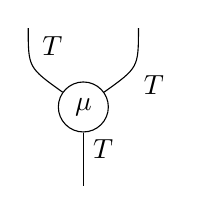
\begin{tikzpicture}[baseline=(current bounding box.center),x=0.7cm]
\path coordinate[] (tikzsd_internal_pos_0_0) at (0.0,0.0);
\path coordinate[] (tikzsd_internal_pos_0_1) at (2.0,0.0);
\path coordinate[] (tikzsd_internal_pos_1_0) at (1.0,-2.0);

\path node[circle,draw,] (tikzsd_internal_nt_node_0_0) at (1.0,-1.0) {$\mu$};

\path [draw] (tikzsd_internal_pos_0_0) ..controls(0.0,-0.5)..(tikzsd_internal_nt_node_0_0) node[pos=0.5,auto,] {$T$};
\path [draw] (tikzsd_internal_pos_0_1) ..controls(2.0,-0.5)..(tikzsd_internal_nt_node_0_0) node[pos=0.5,auto,] {$T$};
\path [draw] (tikzsd_internal_nt_node_0_0) ..controls(1.0,-1.5)..(tikzsd_internal_pos_1_0) node[pos=0.5,auto,] {$T$};
\end{tikzpicture}
    .
\]
The equalities can then be written as
\[
    \begin{tikzpicture}[baseline=(current bounding box.center),y=0.8cm,x=0.6cm]
\path coordinate[] (tikzsd_internal_pos_0_0) at (2.0,0.0);
\path coordinate[] (tikzsd_internal_pos_1_0) at (0.0,-2.0);
\path coordinate[] (tikzsd_internal_pos_1_1) at (2.0,-2.0);
\path coordinate[] (tikzsd_internal_pos_2_0) at (1.0,-4.0);
\path coordinate[] (tikzsd_internal_pos_3_0) at (1.0,-6.0);

\path node[utriangle,draw,] (tikzsd_internal_nt_node_0_0) at (0.0,-1.0) {$\eta$};
\path node[circle,draw,] (tikzsd_internal_nt_node_1_0) at (1.0,-3.0) {$\mu$};

\path [draw] (tikzsd_internal_nt_node_0_0) ..controls(0.0,-1.5)..(tikzsd_internal_pos_1_0) ..controls(0.0,-2.5)..(tikzsd_internal_nt_node_1_0) node[pos=0.0,auto,] {$T$};
\path [draw] (tikzsd_internal_pos_0_0) ..controls(2.0,-0.5)and(2.0,-1.5)..(tikzsd_internal_pos_1_1) node[pos=0.75,auto,] {$T$} ..controls(2.0,-2.5)..(tikzsd_internal_nt_node_1_0);
\path [draw] (tikzsd_internal_nt_node_1_0) ..controls(1.0,-3.5)..(tikzsd_internal_pos_2_0) ..controls(1.0,-4.5)and(1.0,-5.5)..(tikzsd_internal_pos_3_0) node[pos=0.25,auto,] {$T$};
\end{tikzpicture}
    \quad
    =
    \quad
    \begin{tikzpicture}[baseline=(current bounding box.center),y=0.8cm]
\path coordinate[] (tikzsd_internal_pos_0_0) at (0.0,0.0);
\path coordinate[] (tikzsd_internal_pos_1_0) at (0.0,-2.0);
\path coordinate[] (tikzsd_internal_pos_2_0) at (0.0,-4.0);
\path coordinate[] (tikzsd_internal_pos_3_0) at (0.0,-6.0);



\path [draw] (tikzsd_internal_pos_0_0) ..controls(0.0,-0.5)and(0.0,-1.5)..(tikzsd_internal_pos_1_0) ..controls(0.0,-2.5)and(0.0,-3.5)..(tikzsd_internal_pos_2_0) node[pos=0.5,auto,] {$T$} ..controls(0.0,-4.5)and(0.0,-5.5)..(tikzsd_internal_pos_3_0);
\end{tikzpicture}
    \quad
    =
    \quad
    \begin{tikzpicture}[baseline=(current bounding box.center),y=0.8cm,x=0.6cm]
\path coordinate[] (tikzsd_internal_pos_0_0) at (0.0,0.0);
\path coordinate[] (tikzsd_internal_pos_1_0) at (0.0,-2.0);
\path coordinate[] (tikzsd_internal_pos_1_1) at (2.0,-2.0);
\path coordinate[] (tikzsd_internal_pos_2_0) at (1.0,-4.0);
\path coordinate[] (tikzsd_internal_pos_3_0) at (1.0,-6.0);

\path node[utriangle,draw,] (tikzsd_internal_nt_node_0_0) at (2.0,-1.0) {$\eta$};
\path node[circle,draw,] (tikzsd_internal_nt_node_1_0) at (1.0,-3.0) {$\mu$};

\path [draw] (tikzsd_internal_pos_0_0) ..controls(0.0,-0.5)and(0.0,-1.5)..(tikzsd_internal_pos_1_0) node[pos=0.75,auto,] {$T$} ..controls(0.0,-2.5)..(tikzsd_internal_nt_node_1_0);
\path [draw] (tikzsd_internal_nt_node_0_0) ..controls(2.0,-1.5)..(tikzsd_internal_pos_1_1) ..controls(2.0,-2.5)..(tikzsd_internal_nt_node_1_0) node[pos=0.0,auto,] {$T$};
\path [draw] (tikzsd_internal_nt_node_1_0) ..controls(1.0,-3.5)..(tikzsd_internal_pos_2_0) ..controls(1.0,-4.5)and(1.0,-5.5)..(tikzsd_internal_pos_3_0) node[pos=0.25,auto,] {$T$};
\end{tikzpicture}
    \qquad\text{and}\qquad
    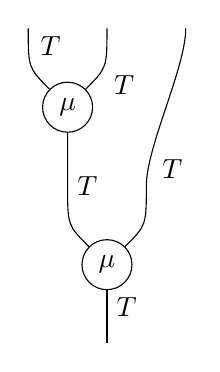
\begin{tikzpicture}[baseline=(current bounding box.center),x=0.5cm]
\path coordinate[] (tikzsd_internal_pos_0_0) at (0.0,0.0);
\path coordinate[] (tikzsd_internal_pos_0_1) at (2.0,0.0);
\path coordinate[] (tikzsd_internal_pos_0_2) at (4.0,0.0);
\path coordinate[] (tikzsd_internal_pos_1_0) at (1.0,-2.0);
\path coordinate[] (tikzsd_internal_pos_1_1) at (3.0,-2.0);
\path coordinate[] (tikzsd_internal_pos_2_0) at (2.0,-4.0);

\path node[circle,draw,] (tikzsd_internal_nt_node_0_0) at (1.0,-1.0) {$\mu$};
\path node[circle,draw,] (tikzsd_internal_nt_node_1_0) at (2.0,-3.0) {$\mu$};

\path [draw] (tikzsd_internal_pos_0_0) ..controls(0.0,-0.5)..(tikzsd_internal_nt_node_0_0) node[pos=0.5,auto,] {$T$};
\path [draw] (tikzsd_internal_pos_0_1) ..controls(2.0,-0.5)..(tikzsd_internal_nt_node_0_0) node[pos=0.5,auto,] {$T$};
\path [draw] (tikzsd_internal_nt_node_0_0) ..controls(1.0,-1.5)..(tikzsd_internal_pos_1_0) ..controls(1.0,-2.5)..(tikzsd_internal_nt_node_1_0) node[pos=0.0,auto,] {$T$};
\path [draw] (tikzsd_internal_pos_0_2) ..controls(4.0,-0.5)and(3.0,-1.5)..(tikzsd_internal_pos_1_1) node[pos=0.75,auto,] {$T$} ..controls(3.0,-2.5)..(tikzsd_internal_nt_node_1_0);
\path [draw] (tikzsd_internal_nt_node_1_0) ..controls(2.0,-3.5)..(tikzsd_internal_pos_2_0) node[pos=0.5,auto,] {$T$};
\end{tikzpicture}
    \quad=\quad
    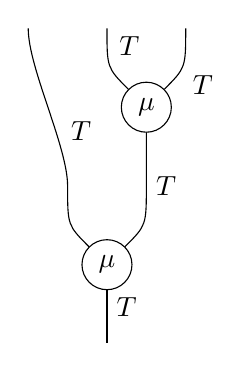
\begin{tikzpicture}[baseline=(current bounding box.center),x=0.5cm]
\path coordinate[] (tikzsd_internal_pos_0_0) at (0.0,0.0);
\path coordinate[] (tikzsd_internal_pos_0_1) at (2.0,0.0);
\path coordinate[] (tikzsd_internal_pos_0_2) at (4.0,0.0);
\path coordinate[] (tikzsd_internal_pos_1_0) at (1.0,-2.0);
\path coordinate[] (tikzsd_internal_pos_1_1) at (3.0,-2.0);
\path coordinate[] (tikzsd_internal_pos_2_0) at (2.0,-4.0);

\path node[circle,draw,] (tikzsd_internal_nt_node_0_0) at (3.0,-1.0) {$\mu$};
\path node[circle,draw,] (tikzsd_internal_nt_node_1_0) at (2.0,-3.0) {$\mu$};

\path [draw] (tikzsd_internal_pos_0_0) ..controls(0.0,-0.5)and(1.0,-1.5)..(tikzsd_internal_pos_1_0) node[pos=0.75,auto,] {$T$} ..controls(1.0,-2.5)..(tikzsd_internal_nt_node_1_0);
\path [draw] (tikzsd_internal_pos_0_1) ..controls(2.0,-0.5)..(tikzsd_internal_nt_node_0_0) node[pos=0.5,auto,] {$T$};
\path [draw] (tikzsd_internal_pos_0_2) ..controls(4.0,-0.5)..(tikzsd_internal_nt_node_0_0) node[pos=0.5,auto,] {$T$};
\path [draw] (tikzsd_internal_nt_node_0_0) ..controls(3.0,-1.5)..(tikzsd_internal_pos_1_1) ..controls(3.0,-2.5)..(tikzsd_internal_nt_node_1_0) node[pos=0.0,auto,] {$T$};
\path [draw] (tikzsd_internal_nt_node_1_0) ..controls(2.0,-3.5)..(tikzsd_internal_pos_2_0) node[pos=0.5,auto,] {$T$};
\end{tikzpicture}
    .
\]
\begin{example} \label{monad-from-adjunction}
    If $(\mc C, \mc D, F, G, \eta, \epsilon)$ is an adjoint pair, then
        $T=G\circ F$ is an endofunctor of $\mc C$
        which can be made into a monad via the following diagrams:
\[
    \begin{tikzpicture}[baseline=(current bounding box.center),]
\path coordinate[] (tikzsd_internal_pos_1_0) at (0.0,-2.0);

\path node[utriangle,draw,] (tikzsd_internal_nt_node_0_0) at (0.0,-1.0) {$\eta$};

\path [draw] (tikzsd_internal_nt_node_0_0) ..controls(0.0,-1.5)..(tikzsd_internal_pos_1_0) node[pos=0.5,auto,] {$T$};
\end{tikzpicture}
    =
    \begin{tikzpicture}[baseline=(current bounding box.center),]
\path coordinate[] (tikzsd_internal_pos_1_0) at (0.0,-2.0);
\path coordinate[] (tikzsd_internal_pos_1_1) at (1.0,-2.0);

\path node[utriangle,draw,] (tikzsd_internal_nt_node_0_0) at (0.5,-1.0) {$\eta$};

\path [draw] (tikzsd_internal_nt_node_0_0) ..controls(0.0,-1.5)..(tikzsd_internal_pos_1_0) node[pos=0.5,auto,] {$F$};
\path [draw] (tikzsd_internal_nt_node_0_0) ..controls(1.0,-1.5)..(tikzsd_internal_pos_1_1) node[pos=0.5,auto,] {$G$};
\end{tikzpicture}
    \qquad\text{and}\qquad
    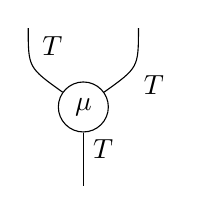
\begin{tikzpicture}[baseline=(current bounding box.center),x=0.7cm]
\path coordinate[] (tikzsd_internal_pos_0_0) at (0.0,0.0);
\path coordinate[] (tikzsd_internal_pos_0_1) at (2.0,0.0);
\path coordinate[] (tikzsd_internal_pos_1_0) at (1.0,-2.0);

\path node[circle,draw,] (tikzsd_internal_nt_node_0_0) at (1.0,-1.0) {$\mu$};

\path [draw] (tikzsd_internal_pos_0_0) ..controls(0.0,-0.5)..(tikzsd_internal_nt_node_0_0) node[pos=0.5,auto,] {$T$};
\path [draw] (tikzsd_internal_pos_0_1) ..controls(2.0,-0.5)..(tikzsd_internal_nt_node_0_0) node[pos=0.5,auto,] {$T$};
\path [draw] (tikzsd_internal_nt_node_0_0) ..controls(1.0,-1.5)..(tikzsd_internal_pos_1_0) node[pos=0.5,auto,] {$T$};
\end{tikzpicture}
    =
    \begin{tikzpicture}[baseline=(current bounding box.center),]
\path coordinate[] (tikzsd_internal_pos_0_0) at (0.0,0.0);
\path coordinate[] (tikzsd_internal_pos_0_1) at (1.0,0.0);
\path coordinate[] (tikzsd_internal_pos_0_2) at (2.0,0.0);
\path coordinate[] (tikzsd_internal_pos_0_3) at (3.0,0.0);
\path coordinate[] (tikzsd_internal_pos_1_0) at (1.0,-2.0);
\path coordinate[] (tikzsd_internal_pos_1_1) at (2.0,-2.0);

\path node[btriangle,draw,] (tikzsd_internal_nt_node_0_0) at (1.5,-1.0) {$\epsilon$};

\path [draw] (tikzsd_internal_pos_0_0) ..controls(0.0,-0.5)and(1.0,-1.5)..(tikzsd_internal_pos_1_0) node[pos=0.5,auto,] {$F$};
\path [draw] (tikzsd_internal_pos_0_1) ..controls(1.0,-0.5)..(tikzsd_internal_nt_node_0_0) node[pos=0.5,auto,] {$G$};
\path [draw] (tikzsd_internal_pos_0_2) ..controls(2.0,-0.5)..(tikzsd_internal_nt_node_0_0) node[pos=0.5,auto,] {$F$};
\path [draw] (tikzsd_internal_pos_0_3) ..controls(3.0,-0.5)and(2.0,-1.5)..(tikzsd_internal_pos_1_1) node[pos=0.5,auto,] {$G$};
\end{tikzpicture}
    .
\]
Note here that there is no ambiguity between the two meanings of $\eta$.
One can check the axioms:
\[
    \begin{tikzpicture}[baseline=(current bounding box.center),]
\path coordinate[] (tikzsd_internal_pos_0_0) at (2.0,0.0);
\path coordinate[] (tikzsd_internal_pos_0_1) at (3.0,0.0);
\path coordinate[] (tikzsd_internal_pos_1_0) at (0.0,-2.0);
\path coordinate[] (tikzsd_internal_pos_1_1) at (1.0,-2.0);
\path coordinate[] (tikzsd_internal_pos_1_2) at (2.0,-2.0);
\path coordinate[] (tikzsd_internal_pos_1_3) at (3.0,-2.0);
\path coordinate[] (tikzsd_internal_pos_2_0) at (1.0,-4.0);
\path coordinate[] (tikzsd_internal_pos_2_1) at (2.0,-4.0);

\path node[utriangle,draw,] (tikzsd_internal_nt_node_0_0) at (0.5,-1.0) {$\eta$};
\path node[btriangle,draw,] (tikzsd_internal_nt_node_1_0) at (1.5,-3.0) {$\epsilon$};

\path [draw] (tikzsd_internal_nt_node_0_0) ..controls(0.0,-1.5)..(tikzsd_internal_pos_1_0) ..controls(0.0,-2.5)and(1.0,-3.5)..(tikzsd_internal_pos_2_0) node[pos=0.25,auto,] {$F$};
\path [draw] (tikzsd_internal_nt_node_0_0) ..controls(1.0,-1.5)..(tikzsd_internal_pos_1_1) ..controls(1.0,-2.5)..(tikzsd_internal_nt_node_1_0) node[pos=0.0,auto,] {$G$};
\path [draw] (tikzsd_internal_pos_0_0) ..controls(2.0,-0.5)and(2.0,-1.5)..(tikzsd_internal_pos_1_2) node[pos=0.75,auto,] {$F$} ..controls(2.0,-2.5)..(tikzsd_internal_nt_node_1_0);
\path [draw] (tikzsd_internal_pos_0_1) ..controls(3.0,-0.5)and(3.0,-1.5)..(tikzsd_internal_pos_1_3) ..controls(3.0,-2.5)and(2.0,-3.5)..(tikzsd_internal_pos_2_1) node[pos=0.0,auto,] {$G$};
\end{tikzpicture}
    \quad=\quad
    \begin{tikzpicture}[baseline=(current bounding box.center),]
\path coordinate[] (tikzsd_internal_pos_0_0) at (0.0,0.0);
\path coordinate[] (tikzsd_internal_pos_0_1) at (1.0,0.0);
\path coordinate[] (tikzsd_internal_pos_1_0) at (0.0,-2.0);
\path coordinate[] (tikzsd_internal_pos_1_1) at (1.0,-2.0);
\path coordinate[] (tikzsd_internal_pos_2_0) at (0.0,-4.0);
\path coordinate[] (tikzsd_internal_pos_2_1) at (1.0,-4.0);



\path [draw] (tikzsd_internal_pos_0_0) ..controls(0.0,-0.5)and(0.0,-1.5)..(tikzsd_internal_pos_1_0) ..controls(0.0,-2.5)and(0.0,-3.5)..(tikzsd_internal_pos_2_0) node[pos=0.0,auto,] {$F$};
\path [draw] (tikzsd_internal_pos_0_1) ..controls(1.0,-0.5)and(1.0,-1.5)..(tikzsd_internal_pos_1_1) ..controls(1.0,-2.5)and(1.0,-3.5)..(tikzsd_internal_pos_2_1) node[pos=0.0,auto,] {$G$};
\end{tikzpicture}
    \quad=\quad
    \begin{tikzpicture}[baseline=(current bounding box.center),]
\path coordinate[] (tikzsd_internal_pos_0_0) at (0.0,0.0);
\path coordinate[] (tikzsd_internal_pos_0_1) at (1.0,0.0);
\path coordinate[] (tikzsd_internal_pos_1_0) at (0.0,-2.0);
\path coordinate[] (tikzsd_internal_pos_1_1) at (1.0,-2.0);
\path coordinate[] (tikzsd_internal_pos_1_2) at (2.0,-2.0);
\path coordinate[] (tikzsd_internal_pos_1_3) at (3.0,-2.0);
\path coordinate[] (tikzsd_internal_pos_2_0) at (1.0,-4.0);
\path coordinate[] (tikzsd_internal_pos_2_1) at (2.0,-4.0);

\path node[utriangle,draw,] (tikzsd_internal_nt_node_0_0) at (2.5,-1.0) {$\eta$};
\path node[btriangle,draw,] (tikzsd_internal_nt_node_1_0) at (1.5,-3.0) {$\epsilon$};

\path [draw] (tikzsd_internal_pos_0_0) ..controls(0.0,-0.5)and(0.0,-1.5)..(tikzsd_internal_pos_1_0) ..controls(0.0,-2.5)and(1.0,-3.5)..(tikzsd_internal_pos_2_0) node[pos=0.0,auto,] {$F$};
\path [draw] (tikzsd_internal_pos_0_1) ..controls(1.0,-0.5)and(1.0,-1.5)..(tikzsd_internal_pos_1_1) node[pos=0.75,auto,] {$G$} ..controls(1.0,-2.5)..(tikzsd_internal_nt_node_1_0);
\path [draw] (tikzsd_internal_nt_node_0_0) ..controls(2.0,-1.5)..(tikzsd_internal_pos_1_2) ..controls(2.0,-2.5)..(tikzsd_internal_nt_node_1_0) node[pos=0.0,auto,] {$F$};
\path [draw] (tikzsd_internal_nt_node_0_0) ..controls(3.0,-1.5)..(tikzsd_internal_pos_1_3) ..controls(3.0,-2.5)and(2.0,-3.5)..(tikzsd_internal_pos_2_1) node[pos=0.25,auto,] {$G$};
\end{tikzpicture}
\]
    and
\[
    \begin{tikzpicture}[baseline=(current bounding box.center),]
\path coordinate[] (tikzsd_internal_pos_0_0) at (0.0,0.0);
\path coordinate[] (tikzsd_internal_pos_0_1) at (1.0,0.0);
\path coordinate[] (tikzsd_internal_pos_0_2) at (2.0,0.0);
\path coordinate[] (tikzsd_internal_pos_0_3) at (3.0,0.0);
\path coordinate[] (tikzsd_internal_pos_0_4) at (4.0,0.0);
\path coordinate[] (tikzsd_internal_pos_0_5) at (5.0,0.0);
\path coordinate[] (tikzsd_internal_pos_1_0) at (1.0,-2.0);
\path coordinate[] (tikzsd_internal_pos_1_1) at (2.0,-2.0);
\path coordinate[] (tikzsd_internal_pos_1_2) at (3.0,-2.0);
\path coordinate[] (tikzsd_internal_pos_1_3) at (4.0,-2.0);
\path coordinate[] (tikzsd_internal_pos_2_0) at (2.0,-4.0);
\path coordinate[] (tikzsd_internal_pos_2_1) at (3.0,-4.0);

\path node[btriangle,draw,] (tikzsd_internal_nt_node_0_0) at (1.5,-1.0) {$\epsilon$};
\path node[btriangle,draw,] (tikzsd_internal_nt_node_1_0) at (2.5,-3.0) {$\epsilon$};

\path [draw] (tikzsd_internal_pos_0_0) ..controls(0.0,-0.5)and(1.0,-1.5)..(tikzsd_internal_pos_1_0) ..controls(1.0,-2.5)and(2.0,-3.5)..(tikzsd_internal_pos_2_0) node[pos=0.0,auto,] {$F$};
\path [draw] (tikzsd_internal_pos_0_1) ..controls(1.0,-0.5)..(tikzsd_internal_nt_node_0_0) node[pos=0.5,auto,] {$G$};
\path [draw] (tikzsd_internal_pos_0_2) ..controls(2.0,-0.5)..(tikzsd_internal_nt_node_0_0) node[pos=0.5,auto,] {$F$};
\path [draw] (tikzsd_internal_pos_0_3) ..controls(3.0,-0.5)and(2.0,-1.5)..(tikzsd_internal_pos_1_1) node[pos=0.75,auto,] {$G$} ..controls(2.0,-2.5)..(tikzsd_internal_nt_node_1_0);
\path [draw] (tikzsd_internal_pos_0_4) ..controls(4.0,-0.5)and(3.0,-1.5)..(tikzsd_internal_pos_1_2) node[pos=0.75,auto,] {$F$} ..controls(3.0,-2.5)..(tikzsd_internal_nt_node_1_0);
\path [draw] (tikzsd_internal_pos_0_5) ..controls(5.0,-0.5)and(4.0,-1.5)..(tikzsd_internal_pos_1_3) ..controls(4.0,-2.5)and(3.0,-3.5)..(tikzsd_internal_pos_2_1) node[pos=0.0,auto,] {$G$};
\end{tikzpicture}
    \quad=\quad
    \begin{tikzpicture}[baseline=(current bounding box.center),]
\path coordinate[] (tikzsd_internal_pos_0_0) at (0.0,0.0);
\path coordinate[] (tikzsd_internal_pos_0_1) at (1.0,0.0);
\path coordinate[] (tikzsd_internal_pos_0_2) at (2.0,0.0);
\path coordinate[] (tikzsd_internal_pos_0_3) at (3.0,0.0);
\path coordinate[] (tikzsd_internal_pos_0_4) at (4.0,0.0);
\path coordinate[] (tikzsd_internal_pos_0_5) at (5.0,0.0);
\path coordinate[] (tikzsd_internal_pos_1_0) at (1.0,-2.0);
\path coordinate[] (tikzsd_internal_pos_1_1) at (2.0,-2.0);
\path coordinate[] (tikzsd_internal_pos_1_2) at (3.0,-2.0);
\path coordinate[] (tikzsd_internal_pos_1_3) at (4.0,-2.0);
\path coordinate[] (tikzsd_internal_pos_2_0) at (2.0,-4.0);
\path coordinate[] (tikzsd_internal_pos_2_1) at (3.0,-4.0);

\path node[btriangle,draw,] (tikzsd_internal_nt_node_0_0) at (3.5,-1.0) {$\epsilon$};
\path node[btriangle,draw,] (tikzsd_internal_nt_node_1_0) at (2.5,-3.0) {$\epsilon$};

\path [draw] (tikzsd_internal_pos_0_0) ..controls(0.0,-0.5)and(1.0,-1.5)..(tikzsd_internal_pos_1_0) ..controls(1.0,-2.5)and(2.0,-3.5)..(tikzsd_internal_pos_2_0) node[pos=0.0,auto,] {$F$};
\path [draw] (tikzsd_internal_pos_0_1) ..controls(1.0,-0.5)and(2.0,-1.5)..(tikzsd_internal_pos_1_1) node[pos=0.75,auto,] {$G$} ..controls(2.0,-2.5)..(tikzsd_internal_nt_node_1_0);
\path [draw] (tikzsd_internal_pos_0_2) ..controls(2.0,-0.5)and(3.0,-1.5)..(tikzsd_internal_pos_1_2) node[pos=0.75,auto,] {$F$} ..controls(3.0,-2.5)..(tikzsd_internal_nt_node_1_0);
\path [draw] (tikzsd_internal_pos_0_3) ..controls(3.0,-0.5)..(tikzsd_internal_nt_node_0_0) node[pos=0.5,auto,] {$G$};
\path [draw] (tikzsd_internal_pos_0_4) ..controls(4.0,-0.5)..(tikzsd_internal_nt_node_0_0) node[pos=0.5,auto,] {$F$};
\path [draw] (tikzsd_internal_pos_0_5) ..controls(5.0,-0.5)and(4.0,-1.5)..(tikzsd_internal_pos_1_3) ..controls(4.0,-2.5)and(3.0,-3.5)..(tikzsd_internal_pos_2_1) node[pos=0.0,auto,] {$G$};
\end{tikzpicture}
    .
\]
\end{example}
\begin{definition}
    Let $(\mc C, T,\eta,\mu)$ be a monad.
    An algebra over this monad is a tuple $(c,\alpha)$ where
    \begin{itemize}
        \item $c$ is an object of $\mc C$,
        \item $\alpha:T(c)\to c$ is a morphism
    \end{itemize}
        such that
    \begin{itemize}
        \item $\alpha\circ \eta_c=\id_c$,
        \item $\alpha\circ T\alpha=\alpha\circ \mu_c$.
    \end{itemize}
    If $(c,\alpha)$ and $(c',\alpha')$ are algebras over the monad, then a 
        $T$-algebra morphism
        $(c,\alpha)\to (c',\alpha')$ is a morphism $f:c\to c'$
        such that $\alpha' \circ T(f)= f\circ \alpha$.
    We denote the category of algebras over the monad $T$ by $\mc C^T$.
\end{definition}
We can identify objects $c\in \Obj(\mc C)$ with functors from the singleton
    category to $\mc C$ and
    morphisms between objects as natural transformations between the corresponding
    functors from the singleton category.
Using this identification, the morphism $h$ can be represented by the
    string diagram
\[
    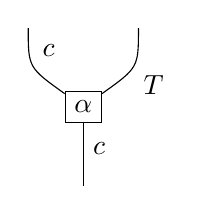
\begin{tikzpicture}[baseline=(current bounding box.center),x=0.7cm]
\path coordinate[] (tikzsd_internal_pos_0_0) at (0.0,0.0);
\path coordinate[] (tikzsd_internal_pos_0_1) at (2.0,0.0);
\path coordinate[] (tikzsd_internal_pos_1_0) at (1.0,-2.0);

\path node[,draw,] (tikzsd_internal_nt_node_0_0) at (1.0,-1.0) {$\alpha$};

\path [draw] (tikzsd_internal_pos_0_0) ..controls(0.0,-0.5)..(tikzsd_internal_nt_node_0_0) node[pos=0.5,auto,] {$c$};
\path [draw] (tikzsd_internal_pos_0_1) ..controls(2.0,-0.5)..(tikzsd_internal_nt_node_0_0) node[pos=0.5,auto,] {$T$};
\path [draw] (tikzsd_internal_nt_node_0_0) ..controls(1.0,-1.5)..(tikzsd_internal_pos_1_0) node[pos=0.5,auto,] {$c$};
\end{tikzpicture}
\]
    and the two equalities can be written as
\[
    \begin{tikzpicture}[baseline=(current bounding box.center),y=0.8cm,x=0.8cm]
\path coordinate[] (tikzsd_internal_pos_0_0) at (0.0,0.0);
\path coordinate[] (tikzsd_internal_pos_1_0) at (0.0,-2.0);
\path coordinate[] (tikzsd_internal_pos_1_1) at (2.0,-2.0);
\path coordinate[] (tikzsd_internal_pos_2_0) at (1.0,-4.0);

\path node[utriangle,draw,] (tikzsd_internal_nt_node_0_0) at (2.0,-1.0) {$\eta$};
\path node[,draw,] (tikzsd_internal_nt_node_1_0) at (1.0,-3.0) {$\alpha$};

\path [draw] (tikzsd_internal_pos_0_0) ..controls(0.0,-0.5)and(0.0,-1.5)..(tikzsd_internal_pos_1_0) node[pos=0.75,auto,] {$c$} ..controls(0.0,-2.5)..(tikzsd_internal_nt_node_1_0);
\path [draw] (tikzsd_internal_nt_node_0_0) ..controls(2.0,-1.5)..(tikzsd_internal_pos_1_1) ..controls(2.0,-2.5)..(tikzsd_internal_nt_node_1_0) node[pos=0.0,auto,] {$T$};
\path [draw] (tikzsd_internal_nt_node_1_0) ..controls(1.0,-3.5)..(tikzsd_internal_pos_2_0) node[pos=0.5,auto,] {$c$};
\end{tikzpicture}
    \quad=\quad
    \begin{tikzpicture}[baseline=(current bounding box.center),y=0.8cm]
\path coordinate[] (tikzsd_internal_pos_0_0) at (0.0,0.0);
\path coordinate[] (tikzsd_internal_pos_1_0) at (0.0,-2.0);
\path coordinate[] (tikzsd_internal_pos_2_0) at (0.0,-4.0);



\path [draw] (tikzsd_internal_pos_0_0) ..controls(0.0,-0.5)and(0.0,-1.5)..(tikzsd_internal_pos_1_0) ..controls(0.0,-2.5)and(0.0,-3.5)..(tikzsd_internal_pos_2_0) node[pos=0.0,auto,] {$c$};
\end{tikzpicture}
    \qquad\text{and}\qquad
    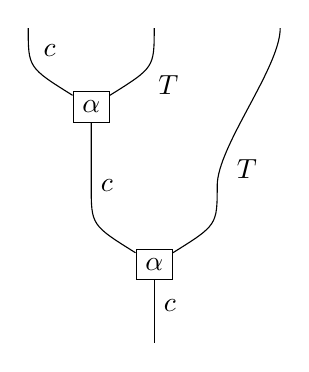
\begin{tikzpicture}[baseline=(current bounding box.center),x=0.8cm]
\path coordinate[] (tikzsd_internal_pos_0_0) at (0.0,0.0);
\path coordinate[] (tikzsd_internal_pos_0_1) at (2.0,0.0);
\path coordinate[] (tikzsd_internal_pos_0_2) at (4.0,0.0);
\path coordinate[] (tikzsd_internal_pos_1_0) at (1.0,-2.0);
\path coordinate[] (tikzsd_internal_pos_1_1) at (3.0,-2.0);
\path coordinate[] (tikzsd_internal_pos_2_0) at (2.0,-4.0);

\path node[,draw,] (tikzsd_internal_nt_node_0_0) at (1.0,-1.0) {$\alpha$};
\path node[,draw,] (tikzsd_internal_nt_node_1_0) at (2.0,-3.0) {$\alpha$};

\path [draw] (tikzsd_internal_pos_0_0) ..controls(0.0,-0.5)..(tikzsd_internal_nt_node_0_0) node[pos=0.5,auto,] {$c$};
\path [draw] (tikzsd_internal_pos_0_1) ..controls(2.0,-0.5)..(tikzsd_internal_nt_node_0_0) node[pos=0.5,auto,] {$T$};
\path [draw] (tikzsd_internal_nt_node_0_0) ..controls(1.0,-1.5)..(tikzsd_internal_pos_1_0) ..controls(1.0,-2.5)..(tikzsd_internal_nt_node_1_0) node[pos=0.0,auto,] {$c$};
\path [draw] (tikzsd_internal_pos_0_2) ..controls(4.0,-0.5)and(3.0,-1.5)..(tikzsd_internal_pos_1_1) node[pos=0.75,auto,] {$T$} ..controls(3.0,-2.5)..(tikzsd_internal_nt_node_1_0);
\path [draw] (tikzsd_internal_nt_node_1_0) ..controls(2.0,-3.5)..(tikzsd_internal_pos_2_0) node[pos=0.5,auto,] {$c$};
\end{tikzpicture}
    \quad=\quad
    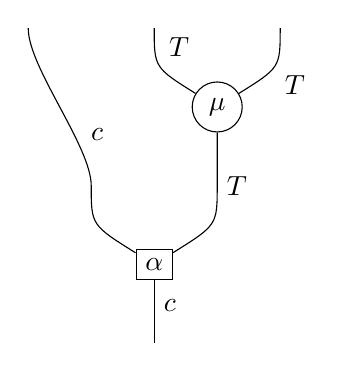
\begin{tikzpicture}[baseline=(current bounding box.center),x=0.8cm]
\path coordinate[] (tikzsd_internal_pos_0_0) at (0.0,0.0);
\path coordinate[] (tikzsd_internal_pos_0_1) at (2.0,0.0);
\path coordinate[] (tikzsd_internal_pos_0_2) at (4.0,0.0);
\path coordinate[] (tikzsd_internal_pos_1_0) at (1.0,-2.0);
\path coordinate[] (tikzsd_internal_pos_1_1) at (3.0,-2.0);
\path coordinate[] (tikzsd_internal_pos_2_0) at (2.0,-4.0);

\path node[circle,draw,] (tikzsd_internal_nt_node_0_0) at (3.0,-1.0) {$\mu$};
\path node[,draw,] (tikzsd_internal_nt_node_1_0) at (2.0,-3.0) {$\alpha$};

\path [draw] (tikzsd_internal_pos_0_0) ..controls(0.0,-0.5)and(1.0,-1.5)..(tikzsd_internal_pos_1_0) node[pos=0.75,auto,] {$c$} ..controls(1.0,-2.5)..(tikzsd_internal_nt_node_1_0);
\path [draw] (tikzsd_internal_pos_0_1) ..controls(2.0,-0.5)..(tikzsd_internal_nt_node_0_0) node[pos=0.5,auto,] {$T$};
\path [draw] (tikzsd_internal_pos_0_2) ..controls(4.0,-0.5)..(tikzsd_internal_nt_node_0_0) node[pos=0.5,auto,] {$T$};
\path [draw] (tikzsd_internal_nt_node_0_0) ..controls(3.0,-1.5)..(tikzsd_internal_pos_1_1) ..controls(3.0,-2.5)..(tikzsd_internal_nt_node_1_0) node[pos=0.0,auto,] {$T$};
\path [draw] (tikzsd_internal_nt_node_1_0) ..controls(2.0,-3.5)..(tikzsd_internal_pos_2_0) node[pos=0.5,auto,] {$c$};
\end{tikzpicture}
    .
\]
\begin{definition}
    Let $(\mc C, \mc D, F, G, \eta, \epsilon)$ be an adjoint pair,
        and let $(\mc C, T, \eta, \mu)$ be the corresponding
        algebra on $\mc C$ as in Example \ref{monad-from-adjunction}.
    Then for every object $d\in \Obj(\mc D)$,
        the object $G(d)\in \Obj(\mc C)$
        where we define
    \[
        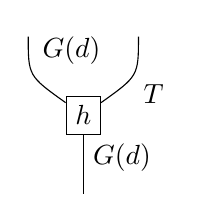
\begin{tikzpicture}[baseline=(current bounding box.center),x=0.7cm]
\path coordinate[] (tikzsd_internal_pos_0_0) at (0.0,0.0);
\path coordinate[] (tikzsd_internal_pos_0_1) at (2.0,0.0);
\path coordinate[] (tikzsd_internal_pos_1_0) at (1.0,-2.0);

\path node[,draw,] (tikzsd_internal_nt_node_0_0) at (1.0,-1.0) {$h$};

\path [draw] (tikzsd_internal_pos_0_0) ..controls(0.0,-0.5)..(tikzsd_internal_nt_node_0_0) node[pos=0.5,auto,] {$G(d)$};
\path [draw] (tikzsd_internal_pos_0_1) ..controls(2.0,-0.5)..(tikzsd_internal_nt_node_0_0) node[pos=0.5,auto,] {$T$};
\path [draw] (tikzsd_internal_nt_node_0_0) ..controls(1.0,-1.5)..(tikzsd_internal_pos_1_0) node[pos=0.5,auto,] {$G(d)$};
\end{tikzpicture}
        \quad=\quad
        \begin{tikzpicture}[baseline=(current bounding box.center),]
\path coordinate[] (tikzsd_internal_pos_0_0) at (0.0,0.0);
\path coordinate[] (tikzsd_internal_pos_0_1) at (1.0,0.0);
\path coordinate[] (tikzsd_internal_pos_0_2) at (2.0,0.0);
\path coordinate[] (tikzsd_internal_pos_0_3) at (3.0,0.0);
\path coordinate[] (tikzsd_internal_pos_1_0) at (1.0,-2.0);
\path coordinate[] (tikzsd_internal_pos_1_1) at (2.0,-2.0);

\path node[btriangle,draw,] (tikzsd_internal_nt_node_0_0) at (1.5,-1.0) {$\epsilon$};

\path [draw] (tikzsd_internal_pos_0_0) ..controls(0.0,-0.5)and(1.0,-1.5)..(tikzsd_internal_pos_1_0) node[pos=0.5,auto,] {$d$};
\path [draw] (tikzsd_internal_pos_0_1) ..controls(1.0,-0.5)..(tikzsd_internal_nt_node_0_0) node[pos=0.5,auto,] {$G$};
\path [draw] (tikzsd_internal_pos_0_2) ..controls(2.0,-0.5)..(tikzsd_internal_nt_node_0_0) node[pos=0.5,auto,] {$F$};
\path [draw] (tikzsd_internal_pos_0_3) ..controls(3.0,-0.5)and(2.0,-1.5)..(tikzsd_internal_pos_1_1) node[pos=0.5,auto,] {$G$};
\end{tikzpicture}
        .
    \]
    We check the equalities
    \[
        \begin{tikzpicture}[baseline=(current bounding box.center),]
\path coordinate[] (tikzsd_internal_pos_0_0) at (0.0,0.0);
\path coordinate[] (tikzsd_internal_pos_0_1) at (1.0,0.0);
\path coordinate[] (tikzsd_internal_pos_1_0) at (0.0,-2.0);
\path coordinate[] (tikzsd_internal_pos_1_1) at (1.0,-2.0);
\path coordinate[] (tikzsd_internal_pos_1_2) at (2.0,-2.0);
\path coordinate[] (tikzsd_internal_pos_1_3) at (3.0,-2.0);
\path coordinate[] (tikzsd_internal_pos_2_0) at (1.0,-4.0);
\path coordinate[] (tikzsd_internal_pos_2_1) at (2.0,-4.0);

\path node[utriangle,draw,] (tikzsd_internal_nt_node_0_0) at (2.5,-1.0) {$\eta$};
\path node[btriangle,draw,] (tikzsd_internal_nt_node_1_0) at (1.5,-3.0) {$\epsilon$};

\path [draw] (tikzsd_internal_pos_0_0) ..controls(0.0,-0.5)and(0.0,-1.5)..(tikzsd_internal_pos_1_0) ..controls(0.0,-2.5)and(1.0,-3.5)..(tikzsd_internal_pos_2_0) node[pos=0.0,auto,] {$d$};
\path [draw] (tikzsd_internal_pos_0_1) ..controls(1.0,-0.5)and(1.0,-1.5)..(tikzsd_internal_pos_1_1) node[pos=0.75,auto,] {$G$} ..controls(1.0,-2.5)..(tikzsd_internal_nt_node_1_0);
\path [draw] (tikzsd_internal_nt_node_0_0) ..controls(2.0,-1.5)..(tikzsd_internal_pos_1_2) ..controls(2.0,-2.5)..(tikzsd_internal_nt_node_1_0) node[pos=0.0,auto,] {$F$};
\path [draw] (tikzsd_internal_nt_node_0_0) ..controls(3.0,-1.5)..(tikzsd_internal_pos_1_3) ..controls(3.0,-2.5)and(2.0,-3.5)..(tikzsd_internal_pos_2_1) node[pos=0.25,auto,] {$G$};
\end{tikzpicture}
        \quad=\quad
        \begin{tikzpicture}[baseline=(current bounding box.center),]
\path coordinate[] (tikzsd_internal_pos_0_0) at (0.0,0.0);
\path coordinate[] (tikzsd_internal_pos_0_1) at (1.0,0.0);
\path coordinate[] (tikzsd_internal_pos_1_0) at (0.0,-2.0);
\path coordinate[] (tikzsd_internal_pos_1_1) at (1.0,-2.0);
\path coordinate[] (tikzsd_internal_pos_2_0) at (0.0,-4.0);
\path coordinate[] (tikzsd_internal_pos_2_1) at (1.0,-4.0);



\path [draw] (tikzsd_internal_pos_0_0) ..controls(0.0,-0.5)and(0.0,-1.5)..(tikzsd_internal_pos_1_0) ..controls(0.0,-2.5)and(0.0,-3.5)..(tikzsd_internal_pos_2_0) node[pos=0.0,auto,] {$d$};
\path [draw] (tikzsd_internal_pos_0_1) ..controls(1.0,-0.5)and(1.0,-1.5)..(tikzsd_internal_pos_1_1) ..controls(1.0,-2.5)and(1.0,-3.5)..(tikzsd_internal_pos_2_1) node[pos=0.0,auto,] {$G$};
\end{tikzpicture}
    \]
    and
    \[
        \begin{tikzpicture}[baseline=(current bounding box.center),]
\path coordinate[] (tikzsd_internal_pos_0_0) at (0.0,0.0);
\path coordinate[] (tikzsd_internal_pos_0_1) at (1.0,0.0);
\path coordinate[] (tikzsd_internal_pos_0_2) at (2.0,0.0);
\path coordinate[] (tikzsd_internal_pos_0_3) at (3.0,0.0);
\path coordinate[] (tikzsd_internal_pos_0_4) at (4.0,0.0);
\path coordinate[] (tikzsd_internal_pos_0_5) at (5.0,0.0);
\path coordinate[] (tikzsd_internal_pos_1_0) at (1.0,-2.0);
\path coordinate[] (tikzsd_internal_pos_1_1) at (2.0,-2.0);
\path coordinate[] (tikzsd_internal_pos_1_2) at (3.0,-2.0);
\path coordinate[] (tikzsd_internal_pos_1_3) at (4.0,-2.0);
\path coordinate[] (tikzsd_internal_pos_2_0) at (2.0,-4.0);
\path coordinate[] (tikzsd_internal_pos_2_1) at (3.0,-4.0);

\path node[btriangle,draw,] (tikzsd_internal_nt_node_0_0) at (1.5,-1.0) {$\epsilon$};
\path node[btriangle,draw,] (tikzsd_internal_nt_node_1_0) at (2.5,-3.0) {$\epsilon$};

\path [draw] (tikzsd_internal_pos_0_0) ..controls(0.0,-0.5)and(1.0,-1.5)..(tikzsd_internal_pos_1_0) ..controls(1.0,-2.5)and(2.0,-3.5)..(tikzsd_internal_pos_2_0) node[pos=0.0,auto,] {$d$};
\path [draw] (tikzsd_internal_pos_0_1) ..controls(1.0,-0.5)..(tikzsd_internal_nt_node_0_0) node[pos=0.5,auto,] {$G$};
\path [draw] (tikzsd_internal_pos_0_2) ..controls(2.0,-0.5)..(tikzsd_internal_nt_node_0_0) node[pos=0.5,auto,] {$F$};
\path [draw] (tikzsd_internal_pos_0_3) ..controls(3.0,-0.5)and(2.0,-1.5)..(tikzsd_internal_pos_1_1) node[pos=0.75,auto,] {$G$} ..controls(2.0,-2.5)..(tikzsd_internal_nt_node_1_0);
\path [draw] (tikzsd_internal_pos_0_4) ..controls(4.0,-0.5)and(3.0,-1.5)..(tikzsd_internal_pos_1_2) node[pos=0.75,auto,] {$F$} ..controls(3.0,-2.5)..(tikzsd_internal_nt_node_1_0);
\path [draw] (tikzsd_internal_pos_0_5) ..controls(5.0,-0.5)and(4.0,-1.5)..(tikzsd_internal_pos_1_3) ..controls(4.0,-2.5)and(3.0,-3.5)..(tikzsd_internal_pos_2_1) node[pos=0.0,auto,] {$G$};
\end{tikzpicture}
        \quad=\quad
        \begin{tikzpicture}[baseline=(current bounding box.center),]
\path coordinate[] (tikzsd_internal_pos_0_0) at (0.0,0.0);
\path coordinate[] (tikzsd_internal_pos_0_1) at (1.0,0.0);
\path coordinate[] (tikzsd_internal_pos_0_2) at (2.0,0.0);
\path coordinate[] (tikzsd_internal_pos_0_3) at (3.0,0.0);
\path coordinate[] (tikzsd_internal_pos_0_4) at (4.0,0.0);
\path coordinate[] (tikzsd_internal_pos_0_5) at (5.0,0.0);
\path coordinate[] (tikzsd_internal_pos_1_0) at (1.0,-2.0);
\path coordinate[] (tikzsd_internal_pos_1_1) at (2.0,-2.0);
\path coordinate[] (tikzsd_internal_pos_1_2) at (3.0,-2.0);
\path coordinate[] (tikzsd_internal_pos_1_3) at (4.0,-2.0);
\path coordinate[] (tikzsd_internal_pos_2_0) at (2.0,-4.0);
\path coordinate[] (tikzsd_internal_pos_2_1) at (3.0,-4.0);

\path node[btriangle,draw,] (tikzsd_internal_nt_node_0_0) at (3.5,-1.0) {$\epsilon$};
\path node[btriangle,draw,] (tikzsd_internal_nt_node_1_0) at (2.5,-3.0) {$\epsilon$};

\path [draw] (tikzsd_internal_pos_0_0) ..controls(0.0,-0.5)and(1.0,-1.5)..(tikzsd_internal_pos_1_0) ..controls(1.0,-2.5)and(2.0,-3.5)..(tikzsd_internal_pos_2_0) node[pos=0.0,auto,] {$d$};
\path [draw] (tikzsd_internal_pos_0_1) ..controls(1.0,-0.5)and(2.0,-1.5)..(tikzsd_internal_pos_1_1) node[pos=0.75,auto,] {$G$} ..controls(2.0,-2.5)..(tikzsd_internal_nt_node_1_0);
\path [draw] (tikzsd_internal_pos_0_2) ..controls(2.0,-0.5)and(3.0,-1.5)..(tikzsd_internal_pos_1_2) node[pos=0.75,auto,] {$F$} ..controls(3.0,-2.5)..(tikzsd_internal_nt_node_1_0);
\path [draw] (tikzsd_internal_pos_0_3) ..controls(3.0,-0.5)..(tikzsd_internal_nt_node_0_0) node[pos=0.5,auto,] {$G$};
\path [draw] (tikzsd_internal_pos_0_4) ..controls(4.0,-0.5)..(tikzsd_internal_nt_node_0_0) node[pos=0.5,auto,] {$F$};
\path [draw] (tikzsd_internal_pos_0_5) ..controls(5.0,-0.5)and(4.0,-1.5)..(tikzsd_internal_pos_1_3) ..controls(4.0,-2.5)and(3.0,-3.5)..(tikzsd_internal_pos_2_1) node[pos=0.0,auto,] {$G$};
\end{tikzpicture}
        .
    \]
    This map $d\mapsto G(d)$ with its algebra structure 
        defines a functor from the category $\mc D$ to the category $\mc C^T$
        of $T$-algebras.

    We say that the adjunction $(\mc C, \mc D, F,G,\eta,\epsilon)$
        is {\em monadic}
        if the morphism $\mc D\to \mc C^T$ is an equivalence of categories.
\end{definition}
\section{Statement of the B\'enabou-Roubaud Theorem}
    In this section, we review the notions of fibrations,
        bifibrations and descent data.
    We then use these concepts to state the B'enabou-Roubaud theorem.
\begin{definition}
    Let $\phi:\mc F \to \mc C$ be a functor.
    We say that a morphism $m:a\to b$ in $\mc F$
        \emph{lies over} the morphism $f:c\to d$ in $\mc C$
        if $\phi(m)=f$.
    
    Given $c\in \Obj(\mc C)$, the \emph{fiber category} over $c$,
        denoted $\mc F(c)$,
        is the category 
    \begin{itemize}
        \item whose objects are the objects $a$ of $\mc F$
            with $\phi(a)=c$,
        \item whose morphisms $f:a\to a'$ 
            between two objects $a,a'$ are the morphisms 
            between these two objects in $\mc F$
            which lie over $\id_c$.
    \end{itemize}
\end{definition}
\begin{definition}
    Let $\phi:\mc F\to \mc C$ be a functor.
    Let $m:a\to b$ in $\mc F$ be a morphism lying over
        $f:c\to d$.
    \begin{itemize}
    \item We say that $m$ is a \emph{cartesian morphism}
        if for every morphism $n:a'\to b$ in $\mc F$ with the same target as $m$ and also lying over $f$,
        there exists a unique morphism $\gamma : a'\to a$
        which lies over $\id_c$
        and satisfies $m\circ \gamma=n$.
    \item Dually, we say that $m$ is a \emph{co-cartesian morphism}
        if for every morphism $n:a\to b'$ in $\mc F$ with the same source as $m$ and also lying over
            $f$,
        there exists a unique morphism $\gamma:b\to b'$
            which lies over $\id_d$ and satisfies $\gamma\circ m=n$.
    \end{itemize}
\end{definition}

\begin{definition}
    A \emph{fibration over $\mc C$} is a functor $\phi:\mc F\to \mc C$ such that 
    \begin{itemize}
    \item any composition of cartesian morphisms is cartesian.
    \item for every
        pair $(b,f:c\to d)$ where $b$ is an object of $\mc F$ and $f:c\to d$ is a morphism
        in $\mc C$ with $d=\phi(b)$,
        there exists a cartesian morphism $m:a\to b$ lying over $f$.
    \end{itemize}

    If $m:f^\ast b\to b$ is such a cartesian morphism, we shall call 
        $(f^\ast b,m)$ an \emph{inverse image} of $b$ under $f$.
    By the properties of cartesian morphisms,
        if $(f^\ast b, m)$ and $((f^\ast b)',m')$ are two inverse images of $b$
        under $f$, then there exists a unique isomorphism $\iota: (f^\ast b)'\to f^\ast b$
        lying over $\id_c$ satisfying $m'=m\circ \iota$.

    If $\phi:\mc F\to \mc C$ is a fibration, then a \emph{choice of inverse images}
        is a choice of inverse image $(f^\ast b,m_{f^\ast b}:f^\ast b\to b)$
        for every pair $(b,f)$ as above.
\end{definition}
\begin{remark}
    Fibrations over $\mc C$ are models of $2$-presheaves on $\mc C$, i.e. contravariant $2$-functors
        from $\mc C$ to the $2$-category of small categories.
    Given a fibration $\phi:\mc F\to \mc C$ 
        such that the fiber categories $\mc F(c)$ are small, along with a choice of inverse images
        $(f,b)\mapsto (f^\ast b, m_{f^\ast b})$, we can define a $2$-functor as follows:
    \begin{itemize}
        \item At the level of objects, we send $c \in \Obj(\mc C)$
            to the category $\mc F(c)$.
        \item At the level of morphisms, if $f:c\to d$ is a morphism in $\mc C$
                and $b$ is an object in $\mc F(d)$, then $f^\ast b$ is an object of $\mc F(c)$.
            Moreover, if $h:b\to b'$ is a morphism in $\mc F(d)$,
                then there exists a unique morphism $f^\ast(h):f^\ast b\to f^\ast b'$
                such that $m_{f^\ast b'}\circ f^\ast(h)=h\circ m_{f^\ast b}$.
            This defines a functor $\mc F(d)\to\mc F(c)$.
        \item At the level of $2$-morphisms, if $f=h\circ g$ in $\mc C$
                and $d$ is the target of this morphism,
                then for any object $b$ of $\mc F(d)$,
                both $(f^\ast b, m_{f^\ast b})$ and 
                $(h^\ast g^\ast b,m_{g^\ast b}\circ m_{h^\ast g^\ast b})$
                are inverse images of $b$ under $f=h\circ g$.
            There is then a unique isomorphism $\iota_b:f^\ast b\to h^\ast g^\ast b$
                with $m_{f^\ast b}= m_{g^\ast b}\circ m_{h^\ast g^\ast b}\circ \iota_b$.
            We have thus described a natural isomorphism between $f^\ast$
                and $h^\ast g^\ast$.
    \end{itemize}
    These definitions will give us a contravariant $2$-functor from $\mc C$ to 
        the $2$-category of small categories.
    Note the fact that in this last point, the functors $f^\ast$ and $h^\ast g^\ast$
        are not the same but rather are naturally isomorphic.
    This is what makes this into a $2$-functor and not a functor.

    On the other hand, one can go backwards: given a $2$-functor from $\mc C$ to the $2$-category of small categories,
        it is possible construct an associated fiber category over $\mc C$.
    We skip this construction.
    Going from a fibration to a $2$-functor back to a fibration yields 
        a fibration over $\mc C$ which is equivalent (in a suitable sense)
        to the original fibration.
    Similarly, going from a $2$-functor to a fibration back to a $2$-functor
        yields a $2$-functor which is equivalent to the orginial one.
\end{remark}
\begin{definition}
    Dually, a \emph{op-fibration} is a functor $\phi:\mc F\to \mc C$ such that
    \begin{itemize}
        \item the composition of co-cartesian morphisms is co-cartesian.
        \item for every pair $(a,f:c\to d)$ where $a$ is an object of $\mc F$
            and $f:c\to d$ is a morphism in $\mc C$ with $d=\phi(a)$,
            there exists a co-cartesian morphism $m:a\to b$ lying over $f$.
    \end{itemize}
    Note that $\phi:\mc F\to \mc C$ being an op-fibration is equivalent to
        $\phi^{\op}:\mc F^{\op}\to \mc C^{\op}$ being a fibration.
    
    If $m:a\to f_\ast a$ is a co-cartesian morphism
        lying over $f$, we say that $(f_\ast a,m)$
        is a direct image of $a$ under $f$.
    Similar to before, two direct images are canonically isomorphic,
        and we can similarly give the notion of a \emph{choice of direct images}.
    Moreover, given a choice of direct images, we can define
        direct image functors $f_\ast:\mc F(c)\to \mc F(d)$
        for every morphism $f:c\to d$ in $\mc C$.
\end{definition}
\begin{definition}
    A \emph{bifibration} $\phi:\mc F \to \mc C$ is a morphism of categories
        such that both $\phi:\mc F\to \mc C$ and $\phi^{\op}:\mc F^{\op}\to \mc C^{\op}$
        are fibrations,
        or equivalently, if $\phi$ is both a fibration and an op-fibration.
\end{definition}
\begin{proposition}
    Suppose $\phi:\mc F\to \mc C$ is a bifibration.
    Pick any choice of inverse images and direct images.
    For morphisms $f:c\to d$ in $\mc C$, let
        $f^\ast:\mc F(d)\to \mc F(c)$
        and $f_\ast:\mc F(c)\to \mc F(d)$ be the corresponding inverse and direct image functors.
    Then for any $a\in \Obj(\mc F(c))$ and $b\in \Obj(\mc F(d))$,
    \[
        \Hom_{\mc F(d)}(f_\ast a, b)
        \cong \Hom_{f}(a,b)
        \cong \Hom_{\mc F(c)}(a,f^\ast b).
    \]
    Here $\Hom_f(a,b)$ denotes the set of morphisms $a\to b$ in $\mc F$ which lie over $f$.
    In particular, we have an adjoint pair $f_\ast \dashv f^\ast$.
\end{proposition}
The given isomorphisms are easy to check from the definitions of pullback and pushforward morphisms.
If $\phi:\mc F\to \mc C$ is a bifibration and $f:a\to b$ is a functor in $\mc C$,
    we shall denote the unit and counit of the adjunction $f_\ast \dashv f^\ast$
    by $\eta_f$ and $\epsilon_f$, respectively.
\begin{remark}
    One sees that bifibrations $\phi: \mc F\to \mc C$ give a contravariant $2$-functors
        from $\mc C$ to the $2$-category of small categories with right adjoints as the morphisms.
    On the other hand, the fibration formed from a contravariant $2$-functor from $\mc C$
        to the $2$-category of small categories with right adjoints as the morphisms is actually a
        bifibration.
    So bifibrations are models of such contravariant functors.
\end{remark}
\begin{definition}
    Suppose $\phi:\mc F \to \mc C$ is a bifibration, and pick a choice of pullbacks and
        pushforwards.
    For any commuting square
    \[
        \begin{tikzcd}
            a \arrow[r,"s"] \arrow[d,"t"]& b \arrow[d,"f"] \\
            c \arrow[r,"g"] & d
        \end{tikzcd}
    \]
        in $\mc C$, we define the \emph{push-pull natural transformation}
        $\PP^{s,t}_{f,g}:t_\ast s^\ast \to g^\ast f_\ast$
        by the string diagram
    \[
        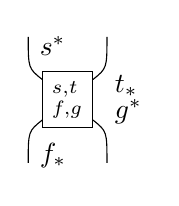
\begin{tikzpicture}[baseline=(current bounding box.center),y=0.8cm]
\path coordinate[] (tikzsd_internal_pos_0_0) at (0.0,0.0);
\path coordinate[] (tikzsd_internal_pos_0_1) at (1.0,0.0);
\path coordinate[] (tikzsd_internal_pos_1_0) at (0.0,-2.0);
\path coordinate[] (tikzsd_internal_pos_1_1) at (1.0,-2.0);

\path node[,draw,] (tikzsd_internal_nt_node_0_0) at (0.5,-1.0) {$\PP^{s,t}_{f,g}$};

\path [draw] (tikzsd_internal_pos_0_0) ..controls(0.0,-0.5)..(tikzsd_internal_nt_node_0_0) node[pos=0.5,auto,] {$s^\ast$};
\path [draw] (tikzsd_internal_pos_0_1) ..controls(1.0,-0.5)..(tikzsd_internal_nt_node_0_0) node[pos=0.5,auto,] {$t_\ast$};
\path [draw] (tikzsd_internal_nt_node_0_0) ..controls(0.0,-1.5)..(tikzsd_internal_pos_1_0) node[pos=0.5,auto,] {$f_\ast$};
\path [draw] (tikzsd_internal_nt_node_0_0) ..controls(1.0,-1.5)..(tikzsd_internal_pos_1_1) node[pos=0.5,auto,] {$g^\ast$};
\end{tikzpicture}
        \quad=\quad
        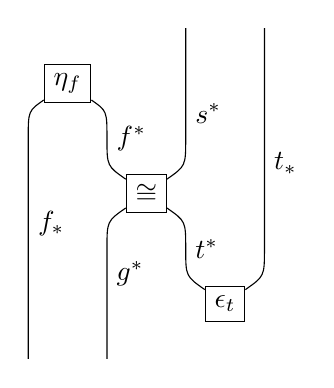
\begin{tikzpicture}[baseline=(current bounding box.center),y=0.7cm]
\path coordinate[] (tikzsd_internal_pos_0_0) at (2.0,0.0);
\path coordinate[] (tikzsd_internal_pos_0_1) at (3.0,0.0);
\path coordinate[] (tikzsd_internal_pos_1_0) at (0.0,-2.0);
\path coordinate[] (tikzsd_internal_pos_1_1) at (1.0,-2.0);
\path coordinate[] (tikzsd_internal_pos_1_2) at (2.0,-2.0);
\path coordinate[] (tikzsd_internal_pos_1_3) at (3.0,-2.0);
\path coordinate[] (tikzsd_internal_pos_2_0) at (0.0,-4.0);
\path coordinate[] (tikzsd_internal_pos_2_1) at (1.0,-4.0);
\path coordinate[] (tikzsd_internal_pos_2_2) at (2.0,-4.0);
\path coordinate[] (tikzsd_internal_pos_2_3) at (3.0,-4.0);
\path coordinate[] (tikzsd_internal_pos_3_0) at (0.0,-6.0);
\path coordinate[] (tikzsd_internal_pos_3_1) at (1.0,-6.0);

\path node[,draw,] (tikzsd_internal_nt_node_0_0) at (0.5,-1.0) {$\eta_f$};
\path node[,draw,] (tikzsd_internal_nt_node_1_0) at (1.5,-3.0) {$\cong$};
\path node[,draw,] (tikzsd_internal_nt_node_2_0) at (2.5,-5.0) {$\epsilon_t$};

\path [draw] (tikzsd_internal_nt_node_0_0) ..controls(0.0,-1.5)..(tikzsd_internal_pos_1_0) ..controls(0.0,-2.5)and(0.0,-3.5)..(tikzsd_internal_pos_2_0) node[pos=0.75,auto,] {$f_\ast$} ..controls(0.0,-4.5)and(0.0,-5.5)..(tikzsd_internal_pos_3_0);
\path [draw] (tikzsd_internal_nt_node_0_0) ..controls(1.0,-1.5)..(tikzsd_internal_pos_1_1) ..controls(1.0,-2.5)..(tikzsd_internal_nt_node_1_0) node[pos=0.0,auto,] {$f^\ast$};
\path [draw] (tikzsd_internal_pos_0_0) ..controls(2.0,-0.5)and(2.0,-1.5)..(tikzsd_internal_pos_1_2) node[pos=0.75,auto,] {$s^\ast$} ..controls(2.0,-2.5)..(tikzsd_internal_nt_node_1_0);
\path [draw] (tikzsd_internal_nt_node_1_0) ..controls(1.0,-3.5)..(tikzsd_internal_pos_2_1) ..controls(1.0,-4.5)and(1.0,-5.5)..(tikzsd_internal_pos_3_1) node[pos=0.25,auto,] {$g^\ast$};
\path [draw] (tikzsd_internal_nt_node_1_0) ..controls(2.0,-3.5)..(tikzsd_internal_pos_2_2) ..controls(2.0,-4.5)..(tikzsd_internal_nt_node_2_0) node[pos=0.0,auto,] {$t^\ast$};
\path [draw] (tikzsd_internal_pos_0_1) ..controls(3.0,-0.5)and(3.0,-1.5)..(tikzsd_internal_pos_1_3) ..controls(3.0,-2.5)and(3.0,-3.5)..(tikzsd_internal_pos_2_3) node[pos=0.25,auto,] {$t_\ast$} ..controls(3.0,-4.5)..(tikzsd_internal_nt_node_2_0);
\end{tikzpicture}
        .
    \]
    The center of the second diagram is the isomorphism $s^\ast f^\ast \cong t^\ast g^\ast$
        coming from the fact that $f\circ s = g\circ t$.
\end{definition}
\begin{definition}[Beck-Chevalley Condition]
    Let $\phi:\mc F\to \mc C$ be a bifibration.
    Pick any choice of inverse and direct images.
    We say that the bifibration satisfies the \emph{Beck-Chevalley condition}
        if for every pullback square 
    \[
        \begin{tikzcd}
            a \arrow[r,"s"] \arrow[d,"t"]& b \arrow[d,"f"] \\
            c \arrow[r,"g"] & d
        \end{tikzcd}
    \]
        in $\mc C$, the push-pull natural transformation $\PP^{s,t}_{f,g}$
        is a natural isomorphism.
\end{definition}
Finally, the last element we need to state the B\'enabou-Roubaud theorem is the notion
    of descent data.
\begin{definition}[Descent Data] \label{def-descent-data}
    Suppose $\phi:\mc F\to \mc C$ is a fibration and suppose $\mc C$
        has all pullbacks.
    Let $f:b\to a$ be a morphism in $\mc C$.
    Let $p_1,p_2:a\times_b a \to a$ denote the two projections,
        and $\pi_1,\pi_2,\pi_3:a\times_b a\times_b a\to a$
        denote the three projections.
    Write $\pi_{ij}=(\pi_i,\pi_j):a\times_b a\times_b a\to a\times_b a$
        for $i,j\in \{1,2,3\}$.

    A \emph{descent datum} relative to $f$ is a pair $(x,\beta)$ where
    \begin{itemize}
        \item $x$ is an object of $\mc F(a)$,
        \item $\beta: p_1^\ast x\to p_2^\ast x$ is an isomorphism,
    \end{itemize}
        such that the following holds:
    \begin{itemize}
        \item if $\tau_{ij}:\pi_i^\ast x\to \pi_j^\ast x$ is
            the composite isomorphism
            \[
                \pi_i^\ast x \cong \pi_{ij}^\ast p_0^\ast x
                \xrightarrow{\beta} \pi_{ij}^\ast p_1^\ast x
                \cong \pi_j^\ast x
            \]
            then $\tau_{13}=\tau_{23}\circ \tau_{12}$.
    \end{itemize}

    The collection of descent data relative to $f$ are the objects of a category
        $\Desc(f)$.
    The collection of morphisms from $(x,\beta_x)$ to $(y,\beta_y)$ is
        the collection of morphisms
        $h:x\to y$ in $\mc F(a)$
        such that $p_1^\ast(h)\circ \beta_x=\beta_y\circ p_0^\ast(h)$.
\end{definition}
\begin{remark}
    The category of descent data relative to $f$ is a model for the
        $2$-limit
        of the diagram
    \[
        \begin{tikzcd}
            \mc F(b) \arrow[r,shift left] \arrow[r,shift right] & \mc F(b\times_a b)
            \arrow[r,shift left=2] \arrow[r] \arrow[r,shift right=2] & \mc F(b\times_a b\times_a b).
        \end{tikzcd}
    \]
    Here, the two morphisms $\mc F(b)\to \mc F(b\times_a b)$ are $p_2^\ast$ and $p_1^\ast$
        and the three morphisms $\mc F(b\times_a b)\to \mc F(b\times_a b\times_a b)$
        are $\pi_{23}^\ast,\pi_{13}^\ast$ and $\pi_{12}^\ast$.
\end{remark}
\begin{example}
    There is a natural functor $\mc F(b)\to \Desc(f)$.
    If $y$ is an object of $\mc F(b)$,
        then $f^\ast y$ is an object of $\mc F(a)$.
    Moreover, since $p_1\circ f = p_2\circ f$ as morphisms $a\times_b a\to b$,
        there is a natural isomorphism $\iota:p_1^\ast f^\ast \cong p_2^\ast f^\ast$.
    Then $(f^\ast y,\iota_y)$ will be a descent datum along $f$.
    This will define our functor $\mc F(b)\to \Desc(f)$.
\end{example}
\begin{definition}
    If $\phi:\mc F\to \mc C$ is a fibration.
    Suppose $\mc C$ has all pullbacks, and let $f:a\to b$ be a morphism in $\mc C$.
    We say that \emph{descent along $f$ is effective}
        if the natural functor $\mc F(b)\to \Desc(f)$ is an equivalence of categories.
\end{definition}
We can now state the B\'enabou-Roubaud result.
\begin{theorem}[B\'enabou-Roubaud]\label{benabou-roubaud}
    Let $\phi:\mc F\to \mc C$ be a bifibration,
        and suppose $\mc C$ has all pullbacks.
    For any morphism $f:b\to a$ in $\mc C$,
        let $(\mc F(b),T,\eta_f,\mu)$
        be the monad
        defined by the adjoint pair $f_\ast \dashv f^\ast$.
    Then 
    \begin{enumerate}
    \item for any $T$-algebra $(x,\alpha:Tx\to x)$, the pair $(x,\beta:p_1^\ast x\to p_2^\ast x)$
        is a descent datum along $f$, where $\beta$ is defined by the string diagram
    \[
        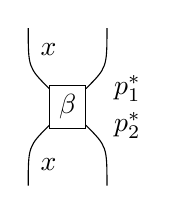
\begin{tikzpicture}[baseline=(current bounding box.center),]
\path coordinate[] (tikzsd_internal_pos_0_0) at (0.0,0.0);
\path coordinate[] (tikzsd_internal_pos_0_1) at (1.0,0.0);
\path coordinate[] (tikzsd_internal_pos_1_0) at (0.0,-2.0);
\path coordinate[] (tikzsd_internal_pos_1_1) at (1.0,-2.0);

\path node[,draw,] (tikzsd_internal_nt_node_0_0) at (0.5,-1.0) {$\beta$};

\path [draw] (tikzsd_internal_pos_0_0) ..controls(0.0,-0.5)..(tikzsd_internal_nt_node_0_0) node[pos=0.5,auto,] {$x$};
\path [draw] (tikzsd_internal_pos_0_1) ..controls(1.0,-0.5)..(tikzsd_internal_nt_node_0_0) node[pos=0.5,auto,] {$p_1^\ast$};
\path [draw] (tikzsd_internal_nt_node_0_0) ..controls(0.0,-1.5)..(tikzsd_internal_pos_1_0) node[pos=0.5,auto,] {$x$};
\path [draw] (tikzsd_internal_nt_node_0_0) ..controls(1.0,-1.5)..(tikzsd_internal_pos_1_1) node[pos=0.5,auto,] {$p_2^\ast$};
\end{tikzpicture}
        \quad=\quad
        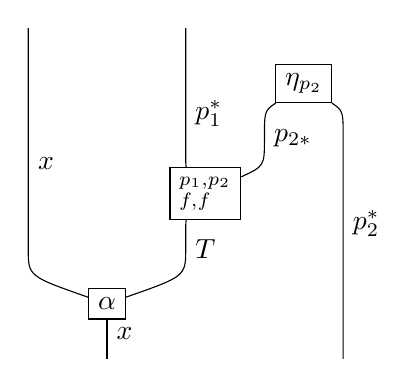
\begin{tikzpicture}[baseline=(current bounding box.center),y=0.7cm]
\path coordinate[] (tikzsd_internal_pos_0_0) at (0.0,0.0);
\path coordinate[] (tikzsd_internal_pos_0_1) at (2.0,0.0);
\path coordinate[] (tikzsd_internal_pos_1_0) at (0.0,-2.0);
\path coordinate[] (tikzsd_internal_pos_1_1) at (2.0,-2.0);
\path coordinate[] (tikzsd_internal_pos_1_2) at (3.0,-2.0);
\path coordinate[] (tikzsd_internal_pos_1_3) at (4.0,-2.0);
\path coordinate[] (tikzsd_internal_pos_2_0) at (0.0,-4.0);
\path coordinate[] (tikzsd_internal_pos_2_1) at (2.0,-4.0);
\path coordinate[] (tikzsd_internal_pos_2_2) at (4.0,-4.0);
\path coordinate[] (tikzsd_internal_pos_3_0) at (1.0,-6.0);
\path coordinate[] (tikzsd_internal_pos_3_1) at (4.0,-6.0);

\path node[,draw,] (tikzsd_internal_nt_node_0_0) at (3.5,-1.0) {$\eta_{p_2}$};
\path node[,draw,] (tikzsd_internal_nt_node_1_0) at (2.25,-3.0) {$\PP^{p_1,p_2}_{f,f}$};
\path node[,draw,] (tikzsd_internal_nt_node_2_0) at (1.0,-5.0) {$\alpha$};

\path [draw] (tikzsd_internal_pos_0_0) ..controls(0.0,-0.5)and(0.0,-1.5)..(tikzsd_internal_pos_1_0) ..controls(0.0,-2.5)and(0.0,-3.5)..(tikzsd_internal_pos_2_0) node[pos=0.25,auto,] {$x$} ..controls(0.0,-4.5)..(tikzsd_internal_nt_node_2_0);
\path [draw] (tikzsd_internal_pos_0_1) ..controls(2.0,-0.5)and(2.0,-1.5)..(tikzsd_internal_pos_1_1) node[pos=0.75,auto,] {$p_1^\ast$} ..controls(2.0,-2.5)..(tikzsd_internal_nt_node_1_0);
\path [draw] (tikzsd_internal_nt_node_0_0) ..controls(3.0,-1.5)..(tikzsd_internal_pos_1_2) ..controls(3.0,-2.5)..(tikzsd_internal_nt_node_1_0) node[pos=0.0,auto,] {$p_{2\ast}$};
\path [draw] (tikzsd_internal_nt_node_1_0) ..controls(2.0,-3.5)..(tikzsd_internal_pos_2_1) ..controls(2.0,-4.5)..(tikzsd_internal_nt_node_2_0) node[pos=0.0,auto,] {$T$};
\path [draw] (tikzsd_internal_nt_node_2_0) ..controls(1.0,-5.5)..(tikzsd_internal_pos_3_0) node[pos=0.5,auto,] {$x$};
\path [draw] (tikzsd_internal_nt_node_0_0) ..controls(4.0,-1.5)..(tikzsd_internal_pos_1_3) ..controls(4.0,-2.5)and(4.0,-3.5)..(tikzsd_internal_pos_2_2) node[pos=0.75,auto,] {$p_2^\ast$} ..controls(4.0,-4.5)and(4.0,-5.5)..(tikzsd_internal_pos_3_1);
\end{tikzpicture}
        .
    \]
    This defines a functor
    \[  
        \mc F(b)^T \to \Desc(f).
    \] \label{benabou-roubaud-functor-def}
    \item There are natural morphisms $\mc F(a)\to \mc F(b)^T$ and $\mc F(a)\to \Desc(f)$
            coming from the properties of adjunctions and the properties of descent data.
        The diagram
    \[
        \begin{tikzcd}
            \mc F(a) \arrow[rd]  \arrow[d] & \\
            \mc F(b)^T \arrow[r] & \Desc(f)
        \end{tikzcd}
    \]
        commutes up to a canonical natural isomorphism.\label{benabou-roubaud-commute}

    \item If $\phi:\mc F\to \mc C$ satisfies the Beck-Chevalley condition, then 
            the functor
            $\mc F(a)^T\to \Desc(f)$ is an equivalence of categories.
\end{enumerate}
\end{theorem}
\begin{remark}
    Actually, under our particular definition of $\Desc(f)$
        in given in \ref{def-descent-data},
        along with our definitions of the functors into $\Desc(f)$,
        the diagram in \eqref{benabou-roubaud-commute}
        commutes, and
        when the Beck-Chevalley condition holds,
        the functor $\mc F(a)^T\to \Desc(f)$ is an isomorphism.
    However, if we think of $\Desc(f)$ as the $2$-limit of a certain diagram,
        then $\Desc(f)$ is only defined up to equivalence of categories,
        and it is only possible to specify functors into $\Desc(f)$
        up to a canonical natural isomorphism.
    This is why we have stated the theorem in the way that we did.
\end{remark}
\begin{corollary}
    Suppose we are in the situation of the B\'enabou-Roubaud theorem,
        and our bifibration satisfies the Beck-Chevalley condition.
    If $f_\ast \dashv f^\ast$ is monadic, then descent along $f$ is effective.
\end{corollary}
\section{The functor $\mc F(b)^T\to \Desc(f)$}
    In this section we show parts \eqref{benabou-roubaud-functor-def} and
    \eqref{benabou-roubaud-commute} of Theorem \ref{benabou-roubaud}.

    For this section, let $(x,\alpha:Tx\to x)$ 
        be a $T$-algebra and let $(x,\beta:p^\ast x\to p_2^\ast x)$
        be defined as in Theorem \ref{benabou-roubaud}\eqref{benabou-roubaud-functor-def}
    Expanding out $\PP^{p_1,p_2}_{f,f}$ in the definition of 
        $\beta$, we see that it is equal to
    \[
        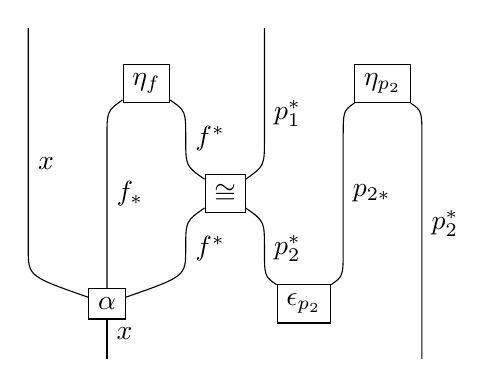
\begin{tikzpicture}[baseline=(current bounding box.center),y=0.7cm]
\path coordinate[] (tikzsd_internal_pos_0_0) at (0.0,0.0);
\path coordinate[] (tikzsd_internal_pos_0_1) at (3.0,0.0);
\path coordinate[] (tikzsd_internal_pos_1_0) at (0.0,-2.0);
\path coordinate[] (tikzsd_internal_pos_1_1) at (1.0,-2.0);
\path coordinate[] (tikzsd_internal_pos_1_2) at (2.0,-2.0);
\path coordinate[] (tikzsd_internal_pos_1_3) at (3.0,-2.0);
\path coordinate[] (tikzsd_internal_pos_1_4) at (4.0,-2.0);
\path coordinate[] (tikzsd_internal_pos_1_5) at (5.0,-2.0);
\path coordinate[] (tikzsd_internal_pos_2_0) at (0.0,-4.0);
\path coordinate[] (tikzsd_internal_pos_2_1) at (1.0,-4.0);
\path coordinate[] (tikzsd_internal_pos_2_2) at (2.0,-4.0);
\path coordinate[] (tikzsd_internal_pos_2_3) at (3.0,-4.0);
\path coordinate[] (tikzsd_internal_pos_2_4) at (4.0,-4.0);
\path coordinate[] (tikzsd_internal_pos_2_5) at (5.0,-4.0);
\path coordinate[] (tikzsd_internal_pos_3_0) at (1.0,-6.0);
\path coordinate[] (tikzsd_internal_pos_3_1) at (5.0,-6.0);

\path node[,draw,] (tikzsd_internal_nt_node_0_0) at (1.5,-1.0) {$\eta_f$};
\path node[,draw,] (tikzsd_internal_nt_node_0_1) at (4.5,-1.0) {$\eta_{p_2}$};
\path node[,draw,] (tikzsd_internal_nt_node_1_0) at (2.5,-3.0) {$\cong$};
\path node[,draw,] (tikzsd_internal_nt_node_2_0) at (1.0,-5.0) {$\alpha$};
\path node[,draw,] (tikzsd_internal_nt_node_2_1) at (3.5,-5.0) {$\epsilon_{p_2}$};

\path [draw] (tikzsd_internal_pos_0_0) ..controls(0.0,-0.5)and(0.0,-1.5)..(tikzsd_internal_pos_1_0) ..controls(0.0,-2.5)and(0.0,-3.5)..(tikzsd_internal_pos_2_0) node[pos=0.25,auto,] {$x$} ..controls(0.0,-4.5)..(tikzsd_internal_nt_node_2_0);
\path [draw] (tikzsd_internal_nt_node_0_0) ..controls(1.0,-1.5)..(tikzsd_internal_pos_1_1) ..controls(1.0,-2.5)and(1.0,-3.5)..(tikzsd_internal_pos_2_1) node[pos=0.5,auto,] {$f_\ast$} ..controls(1.0,-4.5)..(tikzsd_internal_nt_node_2_0);
\path [draw] (tikzsd_internal_nt_node_0_0) ..controls(2.0,-1.5)..(tikzsd_internal_pos_1_2) ..controls(2.0,-2.5)..(tikzsd_internal_nt_node_1_0) node[pos=0.0,auto,] {$f^\ast$};
\path [draw] (tikzsd_internal_pos_0_1) ..controls(3.0,-0.5)and(3.0,-1.5)..(tikzsd_internal_pos_1_3) node[pos=0.75,auto,] {$p_1^\ast$} ..controls(3.0,-2.5)..(tikzsd_internal_nt_node_1_0);
\path [draw] (tikzsd_internal_nt_node_1_0) ..controls(2.0,-3.5)..(tikzsd_internal_pos_2_2) ..controls(2.0,-4.5)..(tikzsd_internal_nt_node_2_0) node[pos=0.0,auto,] {$f^\ast$};
\path [draw] (tikzsd_internal_nt_node_2_0) ..controls(1.0,-5.5)..(tikzsd_internal_pos_3_0) node[pos=0.5,auto,] {$x$};
\path [draw] (tikzsd_internal_nt_node_1_0) ..controls(3.0,-3.5)..(tikzsd_internal_pos_2_3) ..controls(3.0,-4.5)..(tikzsd_internal_nt_node_2_1) node[pos=0.0,auto,] {$p_2^\ast$};
\path [draw] (tikzsd_internal_nt_node_0_1) ..controls(4.0,-1.5)..(tikzsd_internal_pos_1_4) ..controls(4.0,-2.5)and(4.0,-3.5)..(tikzsd_internal_pos_2_4) node[pos=0.5,auto,] {$p_{2\ast}$} ..controls(4.0,-4.5)..(tikzsd_internal_nt_node_2_1);
\path [draw] (tikzsd_internal_nt_node_0_1) ..controls(5.0,-1.5)..(tikzsd_internal_pos_1_5) ..controls(5.0,-2.5)and(5.0,-3.5)..(tikzsd_internal_pos_2_5) node[pos=0.75,auto,] {$p_2^\ast$} ..controls(5.0,-4.5)and(5.0,-5.5)..(tikzsd_internal_pos_3_1);
\end{tikzpicture}
        \quad=\quad
        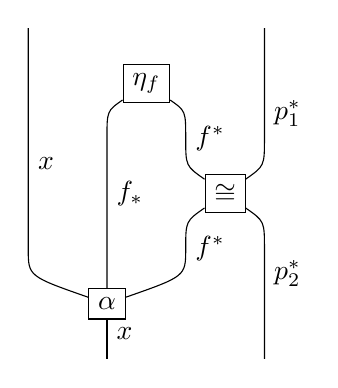
\begin{tikzpicture}[baseline=(current bounding box.center),y=0.7cm]
\path coordinate[] (tikzsd_internal_pos_0_0) at (0.0,0.0);
\path coordinate[] (tikzsd_internal_pos_0_1) at (3.0,0.0);
\path coordinate[] (tikzsd_internal_pos_1_0) at (0.0,-2.0);
\path coordinate[] (tikzsd_internal_pos_1_1) at (1.0,-2.0);
\path coordinate[] (tikzsd_internal_pos_1_2) at (2.0,-2.0);
\path coordinate[] (tikzsd_internal_pos_1_3) at (3.0,-2.0);
\path coordinate[] (tikzsd_internal_pos_2_0) at (0.0,-4.0);
\path coordinate[] (tikzsd_internal_pos_2_1) at (1.0,-4.0);
\path coordinate[] (tikzsd_internal_pos_2_2) at (2.0,-4.0);
\path coordinate[] (tikzsd_internal_pos_2_3) at (3.0,-4.0);
\path coordinate[] (tikzsd_internal_pos_3_0) at (1.0,-6.0);
\path coordinate[] (tikzsd_internal_pos_3_1) at (3.0,-6.0);

\path node[,draw,] (tikzsd_internal_nt_node_0_0) at (1.5,-1.0) {$\eta_f$};
\path node[,draw,] (tikzsd_internal_nt_node_1_0) at (2.5,-3.0) {$\cong$};
\path node[,draw,] (tikzsd_internal_nt_node_2_0) at (1.0,-5.0) {$\alpha$};

\path [draw] (tikzsd_internal_pos_0_0) ..controls(0.0,-0.5)and(0.0,-1.5)..(tikzsd_internal_pos_1_0) ..controls(0.0,-2.5)and(0.0,-3.5)..(tikzsd_internal_pos_2_0) node[pos=0.25,auto,] {$x$} ..controls(0.0,-4.5)..(tikzsd_internal_nt_node_2_0);
\path [draw] (tikzsd_internal_nt_node_0_0) ..controls(1.0,-1.5)..(tikzsd_internal_pos_1_1) ..controls(1.0,-2.5)and(1.0,-3.5)..(tikzsd_internal_pos_2_1) node[pos=0.5,auto,] {$f_\ast$} ..controls(1.0,-4.5)..(tikzsd_internal_nt_node_2_0);
\path [draw] (tikzsd_internal_nt_node_0_0) ..controls(2.0,-1.5)..(tikzsd_internal_pos_1_2) ..controls(2.0,-2.5)..(tikzsd_internal_nt_node_1_0) node[pos=0.0,auto,] {$f^\ast$};
\path [draw] (tikzsd_internal_pos_0_1) ..controls(3.0,-0.5)and(3.0,-1.5)..(tikzsd_internal_pos_1_3) node[pos=0.75,auto,] {$p_1^\ast$} ..controls(3.0,-2.5)..(tikzsd_internal_nt_node_1_0);
\path [draw] (tikzsd_internal_nt_node_1_0) ..controls(2.0,-3.5)..(tikzsd_internal_pos_2_2) ..controls(2.0,-4.5)..(tikzsd_internal_nt_node_2_0) node[pos=0.0,auto,] {$f^\ast$};
\path [draw] (tikzsd_internal_nt_node_2_0) ..controls(1.0,-5.5)..(tikzsd_internal_pos_3_0) node[pos=0.5,auto,] {$x$};
\path [draw] (tikzsd_internal_nt_node_1_0) ..controls(3.0,-3.5)..(tikzsd_internal_pos_2_3) ..controls(3.0,-4.5)and(3.0,-5.5)..(tikzsd_internal_pos_3_1) node[pos=0.25,auto,] {$p_2^\ast$};
\end{tikzpicture}
        .
    \]
\begin{proposition}
    $\beta$ is an isomorphism.
\end{proposition}
    Let $\beta'$ be the morphism $p_2^\ast x\to p_1^\ast x$ gotten by reversing the roles
        of $p_1$ and $p_2$ in the definition of $\beta$, i.e.
    \[
        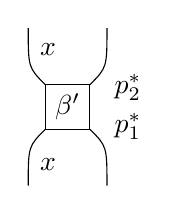
\begin{tikzpicture}[baseline=(current bounding box.center),]
\path coordinate[] (tikzsd_internal_pos_0_0) at (0.0,0.0);
\path coordinate[] (tikzsd_internal_pos_0_1) at (1.0,0.0);
\path coordinate[] (tikzsd_internal_pos_1_0) at (0.0,-2.0);
\path coordinate[] (tikzsd_internal_pos_1_1) at (1.0,-2.0);

\path node[,draw,] (tikzsd_internal_nt_node_0_0) at (0.5,-1.0) {$\beta'$};

\path [draw] (tikzsd_internal_pos_0_0) ..controls(0.0,-0.5)..(tikzsd_internal_nt_node_0_0) node[pos=0.5,auto,] {$x$};
\path [draw] (tikzsd_internal_pos_0_1) ..controls(1.0,-0.5)..(tikzsd_internal_nt_node_0_0) node[pos=0.5,auto,] {$p_2^\ast$};
\path [draw] (tikzsd_internal_nt_node_0_0) ..controls(0.0,-1.5)..(tikzsd_internal_pos_1_0) node[pos=0.5,auto,] {$x$};
\path [draw] (tikzsd_internal_nt_node_0_0) ..controls(1.0,-1.5)..(tikzsd_internal_pos_1_1) node[pos=0.5,auto,] {$p_1^\ast$};
\end{tikzpicture}
        \quad = \quad
        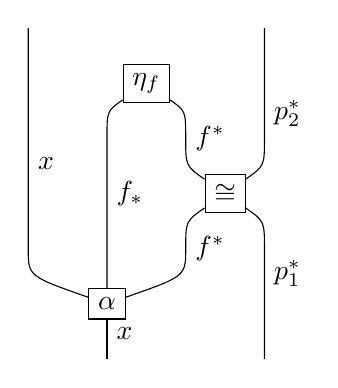
\begin{tikzpicture}[baseline=(current bounding box.center),y=0.7cm]
\path coordinate[] (tikzsd_internal_pos_0_0) at (0.0,0.0);
\path coordinate[] (tikzsd_internal_pos_0_1) at (3.0,0.0);
\path coordinate[] (tikzsd_internal_pos_1_0) at (0.0,-2.0);
\path coordinate[] (tikzsd_internal_pos_1_1) at (1.0,-2.0);
\path coordinate[] (tikzsd_internal_pos_1_2) at (2.0,-2.0);
\path coordinate[] (tikzsd_internal_pos_1_3) at (3.0,-2.0);
\path coordinate[] (tikzsd_internal_pos_2_0) at (0.0,-4.0);
\path coordinate[] (tikzsd_internal_pos_2_1) at (1.0,-4.0);
\path coordinate[] (tikzsd_internal_pos_2_2) at (2.0,-4.0);
\path coordinate[] (tikzsd_internal_pos_2_3) at (3.0,-4.0);
\path coordinate[] (tikzsd_internal_pos_3_0) at (1.0,-6.0);
\path coordinate[] (tikzsd_internal_pos_3_1) at (3.0,-6.0);

\path node[,draw,] (tikzsd_internal_nt_node_0_0) at (1.5,-1.0) {$\eta_f$};
\path node[,draw,] (tikzsd_internal_nt_node_1_0) at (2.5,-3.0) {$\cong$};
\path node[,draw,] (tikzsd_internal_nt_node_2_0) at (1.0,-5.0) {$\alpha$};

\path [draw] (tikzsd_internal_pos_0_0) ..controls(0.0,-0.5)and(0.0,-1.5)..(tikzsd_internal_pos_1_0) ..controls(0.0,-2.5)and(0.0,-3.5)..(tikzsd_internal_pos_2_0) node[pos=0.25,auto,] {$x$} ..controls(0.0,-4.5)..(tikzsd_internal_nt_node_2_0);
\path [draw] (tikzsd_internal_nt_node_0_0) ..controls(1.0,-1.5)..(tikzsd_internal_pos_1_1) ..controls(1.0,-2.5)and(1.0,-3.5)..(tikzsd_internal_pos_2_1) node[pos=0.5,auto,] {$f_\ast$} ..controls(1.0,-4.5)..(tikzsd_internal_nt_node_2_0);
\path [draw] (tikzsd_internal_nt_node_0_0) ..controls(2.0,-1.5)..(tikzsd_internal_pos_1_2) ..controls(2.0,-2.5)..(tikzsd_internal_nt_node_1_0) node[pos=0.0,auto,] {$f^\ast$};
\path [draw] (tikzsd_internal_pos_0_1) ..controls(3.0,-0.5)and(3.0,-1.5)..(tikzsd_internal_pos_1_3) node[pos=0.75,auto,] {$p_2^\ast$} ..controls(3.0,-2.5)..(tikzsd_internal_nt_node_1_0);
\path [draw] (tikzsd_internal_nt_node_1_0) ..controls(2.0,-3.5)..(tikzsd_internal_pos_2_2) ..controls(2.0,-4.5)..(tikzsd_internal_nt_node_2_0) node[pos=0.0,auto,] {$f^\ast$};
\path [draw] (tikzsd_internal_nt_node_2_0) ..controls(1.0,-5.5)..(tikzsd_internal_pos_3_0) node[pos=0.5,auto,] {$x$};
\path [draw] (tikzsd_internal_nt_node_1_0) ..controls(3.0,-3.5)..(tikzsd_internal_pos_2_3) ..controls(3.0,-4.5)and(3.0,-5.5)..(tikzsd_internal_pos_3_1) node[pos=0.25,auto,] {$p_1^\ast$};
\end{tikzpicture}
        .
    \]
    We show that $\beta'$ is an inverse to $\beta$.
    The composition $\beta'\circ \beta$ is given by
    \[
        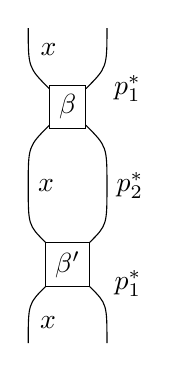
\begin{tikzpicture}[baseline=(current bounding box.center),]
\path coordinate[] (tikzsd_internal_pos_0_0) at (0.0,0.0);
\path coordinate[] (tikzsd_internal_pos_0_1) at (1.0,0.0);
\path coordinate[] (tikzsd_internal_pos_1_0) at (0.0,-2.0);
\path coordinate[] (tikzsd_internal_pos_1_1) at (1.0,-2.0);
\path coordinate[] (tikzsd_internal_pos_2_0) at (0.0,-4.0);
\path coordinate[] (tikzsd_internal_pos_2_1) at (1.0,-4.0);

\path node[,draw,] (tikzsd_internal_nt_node_0_0) at (0.5,-1.0) {$\beta$};
\path node[,draw,] (tikzsd_internal_nt_node_1_0) at (0.5,-3.0) {$\beta'$};

\path [draw] (tikzsd_internal_pos_0_0) ..controls(0.0,-0.5)..(tikzsd_internal_nt_node_0_0) node[pos=0.5,auto,] {$x$};
\path [draw] (tikzsd_internal_pos_0_1) ..controls(1.0,-0.5)..(tikzsd_internal_nt_node_0_0) node[pos=0.5,auto,] {$p_1^\ast$};
\path [draw] (tikzsd_internal_nt_node_0_0) ..controls(0.0,-1.5)..(tikzsd_internal_pos_1_0) ..controls(0.0,-2.5)..(tikzsd_internal_nt_node_1_0) node[pos=0.0,auto,] {$x$};
\path [draw] (tikzsd_internal_nt_node_0_0) ..controls(1.0,-1.5)..(tikzsd_internal_pos_1_1) ..controls(1.0,-2.5)..(tikzsd_internal_nt_node_1_0) node[pos=0.0,auto,] {$p_2^\ast$};
\path [draw] (tikzsd_internal_nt_node_1_0) ..controls(0.0,-3.5)..(tikzsd_internal_pos_2_0) node[pos=0.5,auto,] {$x$};
\path [draw] (tikzsd_internal_nt_node_1_0) ..controls(1.0,-3.5)..(tikzsd_internal_pos_2_1) node[pos=0.5,auto,] {$p_1^\ast$};
\end{tikzpicture}
        \quad = \quad
        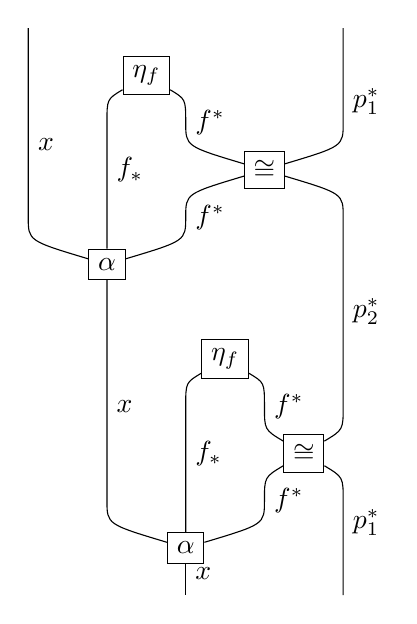
\begin{tikzpicture}[baseline=(current bounding box.center),y=0.6cm]
\path coordinate[] (tikzsd_internal_pos_0_0) at (0.0,0.0);
\path coordinate[] (tikzsd_internal_pos_0_1) at (4.0,0.0);
\path coordinate[] (tikzsd_internal_pos_1_0) at (0.0,-2.0);
\path coordinate[] (tikzsd_internal_pos_1_1) at (1.0,-2.0);
\path coordinate[] (tikzsd_internal_pos_1_2) at (2.0,-2.0);
\path coordinate[] (tikzsd_internal_pos_1_3) at (4.0,-2.0);
\path coordinate[] (tikzsd_internal_pos_2_0) at (0.0,-4.0);
\path coordinate[] (tikzsd_internal_pos_2_1) at (1.0,-4.0);
\path coordinate[] (tikzsd_internal_pos_2_2) at (2.0,-4.0);
\path coordinate[] (tikzsd_internal_pos_2_3) at (4.0,-4.0);
\path coordinate[] (tikzsd_internal_pos_3_0) at (1.0,-6.0);
\path coordinate[] (tikzsd_internal_pos_3_1) at (4.0,-6.0);
\path coordinate[] (tikzsd_internal_pos_4_0) at (1.0,-8.0);
\path coordinate[] (tikzsd_internal_pos_4_1) at (2.0,-8.0);
\path coordinate[] (tikzsd_internal_pos_4_2) at (3.0,-8.0);
\path coordinate[] (tikzsd_internal_pos_4_3) at (4.0,-8.0);
\path coordinate[] (tikzsd_internal_pos_5_0) at (1.0,-10.0);
\path coordinate[] (tikzsd_internal_pos_5_1) at (2.0,-10.0);
\path coordinate[] (tikzsd_internal_pos_5_2) at (3.0,-10.0);
\path coordinate[] (tikzsd_internal_pos_5_3) at (4.0,-10.0);
\path coordinate[] (tikzsd_internal_pos_6_0) at (2.0,-12.0);
\path coordinate[] (tikzsd_internal_pos_6_1) at (4.0,-12.0);

\path node[,draw,] (tikzsd_internal_nt_node_0_0) at (1.5,-1.0) {$\eta_f$};
\path node[,draw,] (tikzsd_internal_nt_node_1_0) at (3.0,-3.0) {$\cong$};
\path node[,draw,] (tikzsd_internal_nt_node_2_0) at (1.0,-5.0) {$\alpha$};
\path node[,draw,] (tikzsd_internal_nt_node_3_0) at (2.5,-7.0) {$\eta_f$};
\path node[,draw,] (tikzsd_internal_nt_node_4_0) at (3.5,-9.0) {$\cong$};
\path node[,draw,] (tikzsd_internal_nt_node_5_0) at (2.0,-11.0) {$\alpha$};

\path [draw] (tikzsd_internal_pos_0_0) ..controls(0.0,-0.5)and(0.0,-1.5)..(tikzsd_internal_pos_1_0) ..controls(0.0,-2.5)and(0.0,-3.5)..(tikzsd_internal_pos_2_0) node[pos=0.25,auto,] {$x$} ..controls(0.0,-4.5)..(tikzsd_internal_nt_node_2_0);
\path [draw] (tikzsd_internal_nt_node_0_0) ..controls(1.0,-1.5)..(tikzsd_internal_pos_1_1) ..controls(1.0,-2.5)and(1.0,-3.5)..(tikzsd_internal_pos_2_1) node[pos=0.5,auto,] {$f_\ast$} ..controls(1.0,-4.5)..(tikzsd_internal_nt_node_2_0);
\path [draw] (tikzsd_internal_nt_node_0_0) ..controls(2.0,-1.5)..(tikzsd_internal_pos_1_2) ..controls(2.0,-2.5)..(tikzsd_internal_nt_node_1_0) node[pos=0.0,auto,] {$f^\ast$};
\path [draw] (tikzsd_internal_pos_0_1) ..controls(4.0,-0.5)and(4.0,-1.5)..(tikzsd_internal_pos_1_3) node[pos=0.75,auto,] {$p_1^\ast$} ..controls(4.0,-2.5)..(tikzsd_internal_nt_node_1_0);
\path [draw] (tikzsd_internal_nt_node_1_0) ..controls(2.0,-3.5)..(tikzsd_internal_pos_2_2) ..controls(2.0,-4.5)..(tikzsd_internal_nt_node_2_0) node[pos=0.0,auto,] {$f^\ast$};
\path [draw] (tikzsd_internal_nt_node_2_0) ..controls(1.0,-5.5)..(tikzsd_internal_pos_3_0) ..controls(1.0,-6.5)and(1.0,-7.5)..(tikzsd_internal_pos_4_0) ..controls(1.0,-8.5)and(1.0,-9.5)..(tikzsd_internal_pos_5_0) node[pos=0.0,auto,] {$x$} ..controls(1.0,-10.5)..(tikzsd_internal_nt_node_5_0);
\path [draw] (tikzsd_internal_nt_node_3_0) ..controls(2.0,-7.5)..(tikzsd_internal_pos_4_1) ..controls(2.0,-8.5)and(2.0,-9.5)..(tikzsd_internal_pos_5_1) node[pos=0.5,auto,] {$f_\ast$} ..controls(2.0,-10.5)..(tikzsd_internal_nt_node_5_0);
\path [draw] (tikzsd_internal_nt_node_3_0) ..controls(3.0,-7.5)..(tikzsd_internal_pos_4_2) ..controls(3.0,-8.5)..(tikzsd_internal_nt_node_4_0) node[pos=0.0,auto,] {$f^\ast$};
\path [draw] (tikzsd_internal_nt_node_1_0) ..controls(4.0,-3.5)..(tikzsd_internal_pos_2_3) ..controls(4.0,-4.5)and(4.0,-5.5)..(tikzsd_internal_pos_3_1) ..controls(4.0,-6.5)and(4.0,-7.5)..(tikzsd_internal_pos_4_3) node[pos=0.0,auto,] {$p_2^\ast$} ..controls(4.0,-8.5)..(tikzsd_internal_nt_node_4_0);
\path [draw] (tikzsd_internal_nt_node_4_0) ..controls(3.0,-9.5)..(tikzsd_internal_pos_5_2) ..controls(3.0,-10.5)..(tikzsd_internal_nt_node_5_0) node[pos=0.0,auto,] {$f^\ast$};
\path [draw] (tikzsd_internal_nt_node_5_0) ..controls(2.0,-11.5)..(tikzsd_internal_pos_6_0) node[pos=0.5,auto,] {$x$};
\path [draw] (tikzsd_internal_nt_node_4_0) ..controls(4.0,-9.5)..(tikzsd_internal_pos_5_3) ..controls(4.0,-10.5)and(4.0,-11.5)..(tikzsd_internal_pos_6_1) node[pos=0.25,auto,] {$p_1^\ast$};
\end{tikzpicture}
        \quad = \quad
        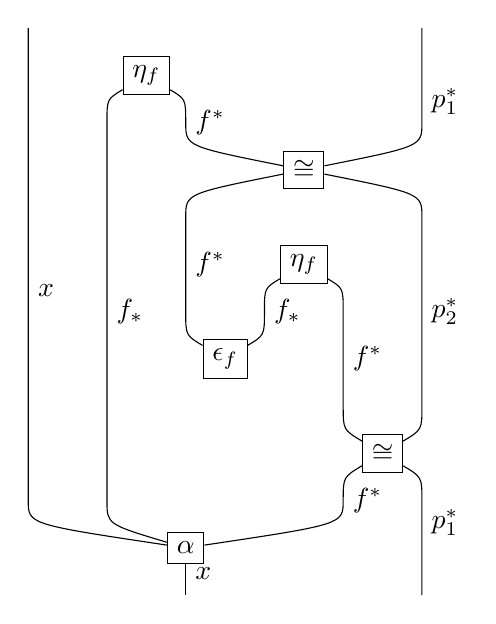
\begin{tikzpicture}[baseline=(current bounding box.center),y=0.6cm]
\path coordinate[] (tikzsd_internal_pos_0_0) at (0.0,0.0);
\path coordinate[] (tikzsd_internal_pos_0_1) at (5.0,0.0);
\path coordinate[] (tikzsd_internal_pos_1_0) at (0.0,-2.0);
\path coordinate[] (tikzsd_internal_pos_1_1) at (1.0,-2.0);
\path coordinate[] (tikzsd_internal_pos_1_2) at (2.0,-2.0);
\path coordinate[] (tikzsd_internal_pos_1_3) at (5.0,-2.0);
\path coordinate[] (tikzsd_internal_pos_2_0) at (0.0,-4.0);
\path coordinate[] (tikzsd_internal_pos_2_1) at (1.0,-4.0);
\path coordinate[] (tikzsd_internal_pos_2_2) at (2.0,-4.0);
\path coordinate[] (tikzsd_internal_pos_2_3) at (5.0,-4.0);
\path coordinate[] (tikzsd_internal_pos_3_0) at (0.0,-6.0);
\path coordinate[] (tikzsd_internal_pos_3_1) at (1.0,-6.0);
\path coordinate[] (tikzsd_internal_pos_3_2) at (2.0,-6.0);
\path coordinate[] (tikzsd_internal_pos_3_3) at (3.0,-6.0);
\path coordinate[] (tikzsd_internal_pos_3_4) at (4.0,-6.0);
\path coordinate[] (tikzsd_internal_pos_3_5) at (5.0,-6.0);
\path coordinate[] (tikzsd_internal_pos_4_0) at (0.0,-8.0);
\path coordinate[] (tikzsd_internal_pos_4_1) at (1.0,-8.0);
\path coordinate[] (tikzsd_internal_pos_4_2) at (4.0,-8.0);
\path coordinate[] (tikzsd_internal_pos_4_3) at (5.0,-8.0);
\path coordinate[] (tikzsd_internal_pos_5_0) at (0.0,-10.0);
\path coordinate[] (tikzsd_internal_pos_5_1) at (1.0,-10.0);
\path coordinate[] (tikzsd_internal_pos_5_2) at (4.0,-10.0);
\path coordinate[] (tikzsd_internal_pos_5_3) at (5.0,-10.0);
\path coordinate[] (tikzsd_internal_pos_6_0) at (2.0,-12.0);
\path coordinate[] (tikzsd_internal_pos_6_1) at (5.0,-12.0);

\path node[,draw,] (tikzsd_internal_nt_node_0_0) at (1.5,-1.0) {$\eta_f$};
\path node[,draw,] (tikzsd_internal_nt_node_1_0) at (3.5,-3.0) {$\cong$};
\path node[,draw,] (tikzsd_internal_nt_node_2_0) at (3.5,-5.0) {$\eta_f$};
\path node[,draw,] (tikzsd_internal_nt_node_3_0) at (2.5,-7.0) {$\epsilon_f$};
\path node[,draw,] (tikzsd_internal_nt_node_4_0) at (4.5,-9.0) {$\cong$};
\path node[,draw,] (tikzsd_internal_nt_node_5_0) at (2.0,-11.0) {$\alpha$};

\path [draw] (tikzsd_internal_pos_0_0) ..controls(0.0,-0.5)and(0.0,-1.5)..(tikzsd_internal_pos_1_0) ..controls(0.0,-2.5)and(0.0,-3.5)..(tikzsd_internal_pos_2_0) ..controls(0.0,-4.5)and(0.0,-5.5)..(tikzsd_internal_pos_3_0) node[pos=0.75,auto,] {$x$} ..controls(0.0,-6.5)and(0.0,-7.5)..(tikzsd_internal_pos_4_0) ..controls(0.0,-8.5)and(0.0,-9.5)..(tikzsd_internal_pos_5_0) ..controls(0.0,-10.5)..(tikzsd_internal_nt_node_5_0);
\path [draw] (tikzsd_internal_nt_node_0_0) ..controls(1.0,-1.5)..(tikzsd_internal_pos_1_1) ..controls(1.0,-2.5)and(1.0,-3.5)..(tikzsd_internal_pos_2_1) ..controls(1.0,-4.5)and(1.0,-5.5)..(tikzsd_internal_pos_3_1) ..controls(1.0,-6.5)and(1.0,-7.5)..(tikzsd_internal_pos_4_1) node[pos=0.0,auto,] {$f_\ast$} ..controls(1.0,-8.5)and(1.0,-9.5)..(tikzsd_internal_pos_5_1) ..controls(1.0,-10.5)..(tikzsd_internal_nt_node_5_0);
\path [draw] (tikzsd_internal_nt_node_0_0) ..controls(2.0,-1.5)..(tikzsd_internal_pos_1_2) ..controls(2.0,-2.5)..(tikzsd_internal_nt_node_1_0) node[pos=0.0,auto,] {$f^\ast$};
\path [draw] (tikzsd_internal_pos_0_1) ..controls(5.0,-0.5)and(5.0,-1.5)..(tikzsd_internal_pos_1_3) node[pos=0.75,auto,] {$p_1^\ast$} ..controls(5.0,-2.5)..(tikzsd_internal_nt_node_1_0);
\path [draw] (tikzsd_internal_nt_node_1_0) ..controls(2.0,-3.5)..(tikzsd_internal_pos_2_2) ..controls(2.0,-4.5)and(2.0,-5.5)..(tikzsd_internal_pos_3_2) node[pos=0.5,auto,] {$f^\ast$} ..controls(2.0,-6.5)..(tikzsd_internal_nt_node_3_0);
\path [draw] (tikzsd_internal_nt_node_2_0) ..controls(3.0,-5.5)..(tikzsd_internal_pos_3_3) ..controls(3.0,-6.5)..(tikzsd_internal_nt_node_3_0) node[pos=0.0,auto,] {$f_\ast$};
\path [draw] (tikzsd_internal_nt_node_2_0) ..controls(4.0,-5.5)..(tikzsd_internal_pos_3_4) ..controls(4.0,-6.5)and(4.0,-7.5)..(tikzsd_internal_pos_4_2) node[pos=0.5,auto,] {$f^\ast$} ..controls(4.0,-8.5)..(tikzsd_internal_nt_node_4_0);
\path [draw] (tikzsd_internal_nt_node_1_0) ..controls(5.0,-3.5)..(tikzsd_internal_pos_2_3) ..controls(5.0,-4.5)and(5.0,-5.5)..(tikzsd_internal_pos_3_5) ..controls(5.0,-6.5)and(5.0,-7.5)..(tikzsd_internal_pos_4_3) node[pos=0.0,auto,] {$p_2^\ast$} ..controls(5.0,-8.5)..(tikzsd_internal_nt_node_4_0);
\path [draw] (tikzsd_internal_nt_node_4_0) ..controls(4.0,-9.5)..(tikzsd_internal_pos_5_2) ..controls(4.0,-10.5)..(tikzsd_internal_nt_node_5_0) node[pos=0.0,auto,] {$f^\ast$};
\path [draw] (tikzsd_internal_nt_node_5_0) ..controls(2.0,-11.5)..(tikzsd_internal_pos_6_0) node[pos=0.5,auto,] {$x$};
\path [draw] (tikzsd_internal_nt_node_4_0) ..controls(5.0,-9.5)..(tikzsd_internal_pos_5_3) ..controls(5.0,-10.5)and(5.0,-11.5)..(tikzsd_internal_pos_6_1) node[pos=0.25,auto,] {$p_1^\ast$};
\end{tikzpicture} \\
    \]
    \[
        \qquad\qquad\qquad=\quad
        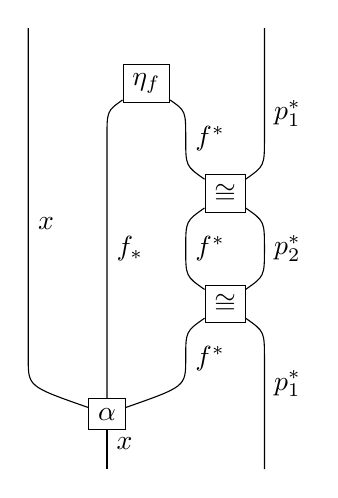
\begin{tikzpicture}[baseline=(current bounding box.center),y=0.7cm]
\path coordinate[] (tikzsd_internal_pos_0_0) at (0.0,0.0);
\path coordinate[] (tikzsd_internal_pos_0_1) at (3.0,0.0);
\path coordinate[] (tikzsd_internal_pos_1_0) at (0.0,-2.0);
\path coordinate[] (tikzsd_internal_pos_1_1) at (1.0,-2.0);
\path coordinate[] (tikzsd_internal_pos_1_2) at (2.0,-2.0);
\path coordinate[] (tikzsd_internal_pos_1_3) at (3.0,-2.0);
\path coordinate[] (tikzsd_internal_pos_2_0) at (0.0,-4.0);
\path coordinate[] (tikzsd_internal_pos_2_1) at (1.0,-4.0);
\path coordinate[] (tikzsd_internal_pos_2_2) at (2.0,-4.0);
\path coordinate[] (tikzsd_internal_pos_2_3) at (3.0,-4.0);
\path coordinate[] (tikzsd_internal_pos_3_0) at (0.0,-6.0);
\path coordinate[] (tikzsd_internal_pos_3_1) at (1.0,-6.0);
\path coordinate[] (tikzsd_internal_pos_3_2) at (2.0,-6.0);
\path coordinate[] (tikzsd_internal_pos_3_3) at (3.0,-6.0);
\path coordinate[] (tikzsd_internal_pos_4_0) at (1.0,-8.0);
\path coordinate[] (tikzsd_internal_pos_4_1) at (3.0,-8.0);

\path node[,draw,] (tikzsd_internal_nt_node_0_0) at (1.5,-1.0) {$\eta_f$};
\path node[,draw,] (tikzsd_internal_nt_node_1_0) at (2.5,-3.0) {$\cong$};
\path node[,draw,] (tikzsd_internal_nt_node_2_0) at (2.5,-5.0) {$\cong$};
\path node[,draw,] (tikzsd_internal_nt_node_3_0) at (1.0,-7.0) {$\alpha$};

\path [draw] (tikzsd_internal_pos_0_0) ..controls(0.0,-0.5)and(0.0,-1.5)..(tikzsd_internal_pos_1_0) ..controls(0.0,-2.5)and(0.0,-3.5)..(tikzsd_internal_pos_2_0) node[pos=0.75,auto,] {$x$} ..controls(0.0,-4.5)and(0.0,-5.5)..(tikzsd_internal_pos_3_0) ..controls(0.0,-6.5)..(tikzsd_internal_nt_node_3_0);
\path [draw] (tikzsd_internal_nt_node_0_0) ..controls(1.0,-1.5)..(tikzsd_internal_pos_1_1) ..controls(1.0,-2.5)and(1.0,-3.5)..(tikzsd_internal_pos_2_1) ..controls(1.0,-4.5)and(1.0,-5.5)..(tikzsd_internal_pos_3_1) node[pos=0.0,auto,] {$f_\ast$} ..controls(1.0,-6.5)..(tikzsd_internal_nt_node_3_0);
\path [draw] (tikzsd_internal_nt_node_0_0) ..controls(2.0,-1.5)..(tikzsd_internal_pos_1_2) ..controls(2.0,-2.5)..(tikzsd_internal_nt_node_1_0) node[pos=0.0,auto,] {$f^\ast$};
\path [draw] (tikzsd_internal_pos_0_1) ..controls(3.0,-0.5)and(3.0,-1.5)..(tikzsd_internal_pos_1_3) node[pos=0.75,auto,] {$p_1^\ast$} ..controls(3.0,-2.5)..(tikzsd_internal_nt_node_1_0);
\path [draw] (tikzsd_internal_nt_node_1_0) ..controls(2.0,-3.5)..(tikzsd_internal_pos_2_2) ..controls(2.0,-4.5)..(tikzsd_internal_nt_node_2_0) node[pos=0.0,auto,] {$f^\ast$};
\path [draw] (tikzsd_internal_nt_node_1_0) ..controls(3.0,-3.5)..(tikzsd_internal_pos_2_3) ..controls(3.0,-4.5)..(tikzsd_internal_nt_node_2_0) node[pos=0.0,auto,] {$p_2^\ast$};
\path [draw] (tikzsd_internal_nt_node_2_0) ..controls(2.0,-5.5)..(tikzsd_internal_pos_3_2) ..controls(2.0,-6.5)..(tikzsd_internal_nt_node_3_0) node[pos=0.0,auto,] {$f^\ast$};
\path [draw] (tikzsd_internal_nt_node_3_0) ..controls(1.0,-7.5)..(tikzsd_internal_pos_4_0) node[pos=0.5,auto,] {$x$};
\path [draw] (tikzsd_internal_nt_node_2_0) ..controls(3.0,-5.5)..(tikzsd_internal_pos_3_3) ..controls(3.0,-6.5)and(3.0,-7.5)..(tikzsd_internal_pos_4_1) node[pos=0.25,auto,] {$p_1^\ast$};
\end{tikzpicture}
        \quad=\quad
        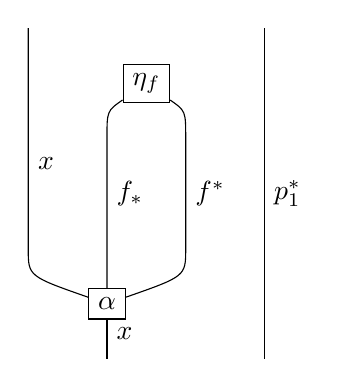
\begin{tikzpicture}[baseline=(current bounding box.center),y=0.7cm]
\path coordinate[] (tikzsd_internal_pos_0_0) at (0.0,0.0);
\path coordinate[] (tikzsd_internal_pos_0_1) at (3.0,0.0);
\path coordinate[] (tikzsd_internal_pos_1_0) at (0.0,-2.0);
\path coordinate[] (tikzsd_internal_pos_1_1) at (1.0,-2.0);
\path coordinate[] (tikzsd_internal_pos_1_2) at (2.0,-2.0);
\path coordinate[] (tikzsd_internal_pos_1_3) at (3.0,-2.0);
\path coordinate[] (tikzsd_internal_pos_2_0) at (0.0,-4.0);
\path coordinate[] (tikzsd_internal_pos_2_1) at (1.0,-4.0);
\path coordinate[] (tikzsd_internal_pos_2_2) at (2.0,-4.0);
\path coordinate[] (tikzsd_internal_pos_2_3) at (3.0,-4.0);
\path coordinate[] (tikzsd_internal_pos_3_0) at (1.0,-6.0);
\path coordinate[] (tikzsd_internal_pos_3_1) at (3.0,-6.0);

\path node[,draw,] (tikzsd_internal_nt_node_0_0) at (1.5,-1.0) {$\eta_f$};
\path node[,draw,] (tikzsd_internal_nt_node_2_0) at (1.0,-5.0) {$\alpha$};

\path [draw] (tikzsd_internal_pos_0_0) ..controls(0.0,-0.5)and(0.0,-1.5)..(tikzsd_internal_pos_1_0) ..controls(0.0,-2.5)and(0.0,-3.5)..(tikzsd_internal_pos_2_0) node[pos=0.25,auto,] {$x$} ..controls(0.0,-4.5)..(tikzsd_internal_nt_node_2_0);
\path [draw] (tikzsd_internal_nt_node_0_0) ..controls(1.0,-1.5)..(tikzsd_internal_pos_1_1) ..controls(1.0,-2.5)and(1.0,-3.5)..(tikzsd_internal_pos_2_1) node[pos=0.5,auto,] {$f_\ast$} ..controls(1.0,-4.5)..(tikzsd_internal_nt_node_2_0);
\path [draw] (tikzsd_internal_nt_node_0_0) ..controls(2.0,-1.5)..(tikzsd_internal_pos_1_2) ..controls(2.0,-2.5)and(2.0,-3.5)..(tikzsd_internal_pos_2_2) node[pos=0.5,auto,] {$f^\ast$} ..controls(2.0,-4.5)..(tikzsd_internal_nt_node_2_0);
\path [draw] (tikzsd_internal_nt_node_2_0) ..controls(1.0,-5.5)..(tikzsd_internal_pos_3_0) node[pos=0.5,auto,] {$x$};
\path [draw] (tikzsd_internal_pos_0_1) ..controls(3.0,-0.5)and(3.0,-1.5)..(tikzsd_internal_pos_1_3) ..controls(3.0,-2.5)and(3.0,-3.5)..(tikzsd_internal_pos_2_3) node[pos=0.5,auto,] {$p_1^\ast$} ..controls(3.0,-4.5)and(3.0,-5.5)..(tikzsd_internal_pos_3_1);
\end{tikzpicture}
        \quad=\quad
        \begin{tikzpicture}[baseline=(current bounding box.center),y=0.7cm]
\path coordinate[] (tikzsd_internal_pos_0_0) at (0.0,0.0);
\path coordinate[] (tikzsd_internal_pos_0_1) at (1.0,0.0);
\path coordinate[] (tikzsd_internal_pos_1_0) at (0.0,-2.0);
\path coordinate[] (tikzsd_internal_pos_1_1) at (1.0,-2.0);
\path coordinate[] (tikzsd_internal_pos_2_0) at (0.0,-4.0);
\path coordinate[] (tikzsd_internal_pos_2_1) at (1.0,-4.0);
\path coordinate[] (tikzsd_internal_pos_3_0) at (0.0,-6.0);
\path coordinate[] (tikzsd_internal_pos_3_1) at (1.0,-6.0);



\path [draw] (tikzsd_internal_pos_0_0) ..controls(0.0,-0.5)and(0.0,-1.5)..(tikzsd_internal_pos_1_0) ..controls(0.0,-2.5)and(0.0,-3.5)..(tikzsd_internal_pos_2_0) node[pos=0.5,auto,] {$x$} ..controls(0.0,-4.5)and(0.0,-5.5)..(tikzsd_internal_pos_3_0);
\path [draw] (tikzsd_internal_pos_0_1) ..controls(1.0,-0.5)and(1.0,-1.5)..(tikzsd_internal_pos_1_1) ..controls(1.0,-2.5)and(1.0,-3.5)..(tikzsd_internal_pos_2_1) node[pos=0.5,auto,] {$p_1^\ast$} ..controls(1.0,-4.5)and(1.0,-5.5)..(tikzsd_internal_pos_3_1);
\end{tikzpicture}
        .
    \]
    We thus see that $\beta'\circ \beta=\id_{p_1^\ast x}$.
    Reversing the roles of $p_1$ and $p_2$ shows that $\beta\circ \beta'=\id_{p_2^\ast x}$,
        so we conclude that $\beta'$ is an inverse to $\beta$.
\begin{proposition}
    In the notation of Definition \ref{def-descent-data},
        $\tau_{13}=\tau_{23}\circ \tau_{12}$.
\end{proposition}
    \begin{align*}
        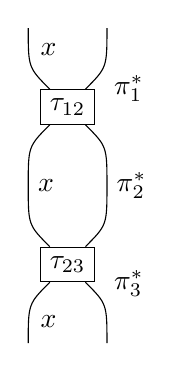
\begin{tikzpicture}[baseline=(current bounding box.center),]
\path coordinate[] (tikzsd_internal_pos_0_0) at (0.0,0.0);
\path coordinate[] (tikzsd_internal_pos_0_1) at (1.0,0.0);
\path coordinate[] (tikzsd_internal_pos_1_0) at (0.0,-2.0);
\path coordinate[] (tikzsd_internal_pos_1_1) at (1.0,-2.0);
\path coordinate[] (tikzsd_internal_pos_2_0) at (0.0,-4.0);
\path coordinate[] (tikzsd_internal_pos_2_1) at (1.0,-4.0);

\path node[,draw,] (tikzsd_internal_nt_node_0_0) at (0.5,-1.0) {$\tau_{12}$};
\path node[,draw,] (tikzsd_internal_nt_node_1_0) at (0.5,-3.0) {$\tau_{23}$};

\path [draw] (tikzsd_internal_pos_0_0) ..controls(0.0,-0.5)..(tikzsd_internal_nt_node_0_0) node[pos=0.5,auto,] {$x$};
\path [draw] (tikzsd_internal_pos_0_1) ..controls(1.0,-0.5)..(tikzsd_internal_nt_node_0_0) node[pos=0.5,auto,] {$\pi_1^\ast$};
\path [draw] (tikzsd_internal_nt_node_0_0) ..controls(0.0,-1.5)..(tikzsd_internal_pos_1_0) ..controls(0.0,-2.5)..(tikzsd_internal_nt_node_1_0) node[pos=0.0,auto,] {$x$};
\path [draw] (tikzsd_internal_nt_node_0_0) ..controls(1.0,-1.5)..(tikzsd_internal_pos_1_1) ..controls(1.0,-2.5)..(tikzsd_internal_nt_node_1_0) node[pos=0.0,auto,] {$\pi_2^\ast$};
\path [draw] (tikzsd_internal_nt_node_1_0) ..controls(0.0,-3.5)..(tikzsd_internal_pos_2_0) node[pos=0.5,auto,] {$x$};
\path [draw] (tikzsd_internal_nt_node_1_0) ..controls(1.0,-3.5)..(tikzsd_internal_pos_2_1) node[pos=0.5,auto,] {$\pi_3^\ast$};
\end{tikzpicture}
        \quad &= \quad
        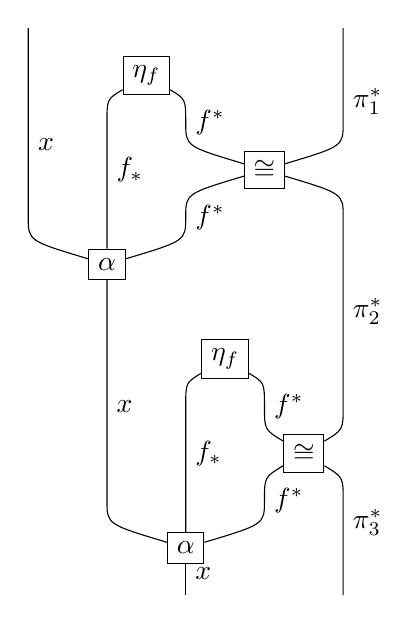
\begin{tikzpicture}[baseline=(current bounding box.center),y=0.6cm]
\path coordinate[] (tikzsd_internal_pos_0_0) at (0.0,0.0);
\path coordinate[] (tikzsd_internal_pos_0_1) at (4.0,0.0);
\path coordinate[] (tikzsd_internal_pos_1_0) at (0.0,-2.0);
\path coordinate[] (tikzsd_internal_pos_1_1) at (1.0,-2.0);
\path coordinate[] (tikzsd_internal_pos_1_2) at (2.0,-2.0);
\path coordinate[] (tikzsd_internal_pos_1_3) at (4.0,-2.0);
\path coordinate[] (tikzsd_internal_pos_2_0) at (0.0,-4.0);
\path coordinate[] (tikzsd_internal_pos_2_1) at (1.0,-4.0);
\path coordinate[] (tikzsd_internal_pos_2_2) at (2.0,-4.0);
\path coordinate[] (tikzsd_internal_pos_2_3) at (4.0,-4.0);
\path coordinate[] (tikzsd_internal_pos_3_0) at (1.0,-6.0);
\path coordinate[] (tikzsd_internal_pos_3_1) at (4.0,-6.0);
\path coordinate[] (tikzsd_internal_pos_4_0) at (1.0,-8.0);
\path coordinate[] (tikzsd_internal_pos_4_1) at (2.0,-8.0);
\path coordinate[] (tikzsd_internal_pos_4_2) at (3.0,-8.0);
\path coordinate[] (tikzsd_internal_pos_4_3) at (4.0,-8.0);
\path coordinate[] (tikzsd_internal_pos_5_0) at (1.0,-10.0);
\path coordinate[] (tikzsd_internal_pos_5_1) at (2.0,-10.0);
\path coordinate[] (tikzsd_internal_pos_5_2) at (3.0,-10.0);
\path coordinate[] (tikzsd_internal_pos_5_3) at (4.0,-10.0);
\path coordinate[] (tikzsd_internal_pos_6_0) at (2.0,-12.0);
\path coordinate[] (tikzsd_internal_pos_6_1) at (4.0,-12.0);

\path node[,draw,] (tikzsd_internal_nt_node_0_0) at (1.5,-1.0) {$\eta_f$};
\path node[,draw,] (tikzsd_internal_nt_node_1_0) at (3.0,-3.0) {$\cong$};
\path node[,draw,] (tikzsd_internal_nt_node_2_0) at (1.0,-5.0) {$\alpha$};
\path node[,draw,] (tikzsd_internal_nt_node_3_0) at (2.5,-7.0) {$\eta_f$};
\path node[,draw,] (tikzsd_internal_nt_node_4_0) at (3.5,-9.0) {$\cong$};
\path node[,draw,] (tikzsd_internal_nt_node_5_0) at (2.0,-11.0) {$\alpha$};

\path [draw] (tikzsd_internal_pos_0_0) ..controls(0.0,-0.5)and(0.0,-1.5)..(tikzsd_internal_pos_1_0) ..controls(0.0,-2.5)and(0.0,-3.5)..(tikzsd_internal_pos_2_0) node[pos=0.25,auto,] {$x$} ..controls(0.0,-4.5)..(tikzsd_internal_nt_node_2_0);
\path [draw] (tikzsd_internal_nt_node_0_0) ..controls(1.0,-1.5)..(tikzsd_internal_pos_1_1) ..controls(1.0,-2.5)and(1.0,-3.5)..(tikzsd_internal_pos_2_1) node[pos=0.5,auto,] {$f_\ast$} ..controls(1.0,-4.5)..(tikzsd_internal_nt_node_2_0);
\path [draw] (tikzsd_internal_nt_node_0_0) ..controls(2.0,-1.5)..(tikzsd_internal_pos_1_2) ..controls(2.0,-2.5)..(tikzsd_internal_nt_node_1_0) node[pos=0.0,auto,] {$f^\ast$};
\path [draw] (tikzsd_internal_pos_0_1) ..controls(4.0,-0.5)and(4.0,-1.5)..(tikzsd_internal_pos_1_3) node[pos=0.75,auto,] {$\pi_1^\ast$} ..controls(4.0,-2.5)..(tikzsd_internal_nt_node_1_0);
\path [draw] (tikzsd_internal_nt_node_1_0) ..controls(2.0,-3.5)..(tikzsd_internal_pos_2_2) ..controls(2.0,-4.5)..(tikzsd_internal_nt_node_2_0) node[pos=0.0,auto,] {$f^\ast$};
\path [draw] (tikzsd_internal_nt_node_2_0) ..controls(1.0,-5.5)..(tikzsd_internal_pos_3_0) ..controls(1.0,-6.5)and(1.0,-7.5)..(tikzsd_internal_pos_4_0) ..controls(1.0,-8.5)and(1.0,-9.5)..(tikzsd_internal_pos_5_0) node[pos=0.0,auto,] {$x$} ..controls(1.0,-10.5)..(tikzsd_internal_nt_node_5_0);
\path [draw] (tikzsd_internal_nt_node_3_0) ..controls(2.0,-7.5)..(tikzsd_internal_pos_4_1) ..controls(2.0,-8.5)and(2.0,-9.5)..(tikzsd_internal_pos_5_1) node[pos=0.5,auto,] {$f_\ast$} ..controls(2.0,-10.5)..(tikzsd_internal_nt_node_5_0);
\path [draw] (tikzsd_internal_nt_node_3_0) ..controls(3.0,-7.5)..(tikzsd_internal_pos_4_2) ..controls(3.0,-8.5)..(tikzsd_internal_nt_node_4_0) node[pos=0.0,auto,] {$f^\ast$};
\path [draw] (tikzsd_internal_nt_node_1_0) ..controls(4.0,-3.5)..(tikzsd_internal_pos_2_3) ..controls(4.0,-4.5)and(4.0,-5.5)..(tikzsd_internal_pos_3_1) ..controls(4.0,-6.5)and(4.0,-7.5)..(tikzsd_internal_pos_4_3) node[pos=0.0,auto,] {$\pi_2^\ast$} ..controls(4.0,-8.5)..(tikzsd_internal_nt_node_4_0);
\path [draw] (tikzsd_internal_nt_node_4_0) ..controls(3.0,-9.5)..(tikzsd_internal_pos_5_2) ..controls(3.0,-10.5)..(tikzsd_internal_nt_node_5_0) node[pos=0.0,auto,] {$f^\ast$};
\path [draw] (tikzsd_internal_nt_node_5_0) ..controls(2.0,-11.5)..(tikzsd_internal_pos_6_0) node[pos=0.5,auto,] {$x$};
\path [draw] (tikzsd_internal_nt_node_4_0) ..controls(4.0,-9.5)..(tikzsd_internal_pos_5_3) ..controls(4.0,-10.5)and(4.0,-11.5)..(tikzsd_internal_pos_6_1) node[pos=0.25,auto,] {$\pi_3^\ast$};
\end{tikzpicture}
        \quad = \quad
        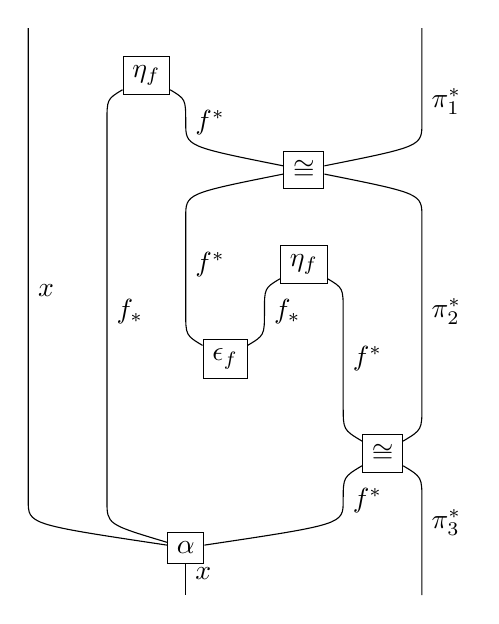
\begin{tikzpicture}[baseline=(current bounding box.center),y=0.6cm]
\path coordinate[] (tikzsd_internal_pos_0_0) at (0.0,0.0);
\path coordinate[] (tikzsd_internal_pos_0_1) at (5.0,0.0);
\path coordinate[] (tikzsd_internal_pos_1_0) at (0.0,-2.0);
\path coordinate[] (tikzsd_internal_pos_1_1) at (1.0,-2.0);
\path coordinate[] (tikzsd_internal_pos_1_2) at (2.0,-2.0);
\path coordinate[] (tikzsd_internal_pos_1_3) at (5.0,-2.0);
\path coordinate[] (tikzsd_internal_pos_2_0) at (0.0,-4.0);
\path coordinate[] (tikzsd_internal_pos_2_1) at (1.0,-4.0);
\path coordinate[] (tikzsd_internal_pos_2_2) at (2.0,-4.0);
\path coordinate[] (tikzsd_internal_pos_2_3) at (5.0,-4.0);
\path coordinate[] (tikzsd_internal_pos_3_0) at (0.0,-6.0);
\path coordinate[] (tikzsd_internal_pos_3_1) at (1.0,-6.0);
\path coordinate[] (tikzsd_internal_pos_3_2) at (2.0,-6.0);
\path coordinate[] (tikzsd_internal_pos_3_3) at (3.0,-6.0);
\path coordinate[] (tikzsd_internal_pos_3_4) at (4.0,-6.0);
\path coordinate[] (tikzsd_internal_pos_3_5) at (5.0,-6.0);
\path coordinate[] (tikzsd_internal_pos_4_0) at (0.0,-8.0);
\path coordinate[] (tikzsd_internal_pos_4_1) at (1.0,-8.0);
\path coordinate[] (tikzsd_internal_pos_4_2) at (4.0,-8.0);
\path coordinate[] (tikzsd_internal_pos_4_3) at (5.0,-8.0);
\path coordinate[] (tikzsd_internal_pos_5_0) at (0.0,-10.0);
\path coordinate[] (tikzsd_internal_pos_5_1) at (1.0,-10.0);
\path coordinate[] (tikzsd_internal_pos_5_2) at (4.0,-10.0);
\path coordinate[] (tikzsd_internal_pos_5_3) at (5.0,-10.0);
\path coordinate[] (tikzsd_internal_pos_6_0) at (2.0,-12.0);
\path coordinate[] (tikzsd_internal_pos_6_1) at (5.0,-12.0);

\path node[,draw,] (tikzsd_internal_nt_node_0_0) at (1.5,-1.0) {$\eta_f$};
\path node[,draw,] (tikzsd_internal_nt_node_1_0) at (3.5,-3.0) {$\cong$};
\path node[,draw,] (tikzsd_internal_nt_node_2_0) at (3.5,-5.0) {$\eta_f$};
\path node[,draw,] (tikzsd_internal_nt_node_3_0) at (2.5,-7.0) {$\epsilon_f$};
\path node[,draw,] (tikzsd_internal_nt_node_4_0) at (4.5,-9.0) {$\cong$};
\path node[,draw,] (tikzsd_internal_nt_node_5_0) at (2.0,-11.0) {$\alpha$};

\path [draw] (tikzsd_internal_pos_0_0) ..controls(0.0,-0.5)and(0.0,-1.5)..(tikzsd_internal_pos_1_0) ..controls(0.0,-2.5)and(0.0,-3.5)..(tikzsd_internal_pos_2_0) ..controls(0.0,-4.5)and(0.0,-5.5)..(tikzsd_internal_pos_3_0) node[pos=0.75,auto,] {$x$} ..controls(0.0,-6.5)and(0.0,-7.5)..(tikzsd_internal_pos_4_0) ..controls(0.0,-8.5)and(0.0,-9.5)..(tikzsd_internal_pos_5_0) ..controls(0.0,-10.5)..(tikzsd_internal_nt_node_5_0);
\path [draw] (tikzsd_internal_nt_node_0_0) ..controls(1.0,-1.5)..(tikzsd_internal_pos_1_1) ..controls(1.0,-2.5)and(1.0,-3.5)..(tikzsd_internal_pos_2_1) ..controls(1.0,-4.5)and(1.0,-5.5)..(tikzsd_internal_pos_3_1) ..controls(1.0,-6.5)and(1.0,-7.5)..(tikzsd_internal_pos_4_1) node[pos=0.0,auto,] {$f_\ast$} ..controls(1.0,-8.5)and(1.0,-9.5)..(tikzsd_internal_pos_5_1) ..controls(1.0,-10.5)..(tikzsd_internal_nt_node_5_0);
\path [draw] (tikzsd_internal_nt_node_0_0) ..controls(2.0,-1.5)..(tikzsd_internal_pos_1_2) ..controls(2.0,-2.5)..(tikzsd_internal_nt_node_1_0) node[pos=0.0,auto,] {$f^\ast$};
\path [draw] (tikzsd_internal_pos_0_1) ..controls(5.0,-0.5)and(5.0,-1.5)..(tikzsd_internal_pos_1_3) node[pos=0.75,auto,] {$\pi_1^\ast$} ..controls(5.0,-2.5)..(tikzsd_internal_nt_node_1_0);
\path [draw] (tikzsd_internal_nt_node_1_0) ..controls(2.0,-3.5)..(tikzsd_internal_pos_2_2) ..controls(2.0,-4.5)and(2.0,-5.5)..(tikzsd_internal_pos_3_2) node[pos=0.5,auto,] {$f^\ast$} ..controls(2.0,-6.5)..(tikzsd_internal_nt_node_3_0);
\path [draw] (tikzsd_internal_nt_node_2_0) ..controls(3.0,-5.5)..(tikzsd_internal_pos_3_3) ..controls(3.0,-6.5)..(tikzsd_internal_nt_node_3_0) node[pos=0.0,auto,] {$f_\ast$};
\path [draw] (tikzsd_internal_nt_node_2_0) ..controls(4.0,-5.5)..(tikzsd_internal_pos_3_4) ..controls(4.0,-6.5)and(4.0,-7.5)..(tikzsd_internal_pos_4_2) node[pos=0.5,auto,] {$f^\ast$} ..controls(4.0,-8.5)..(tikzsd_internal_nt_node_4_0);
\path [draw] (tikzsd_internal_nt_node_1_0) ..controls(5.0,-3.5)..(tikzsd_internal_pos_2_3) ..controls(5.0,-4.5)and(5.0,-5.5)..(tikzsd_internal_pos_3_5) ..controls(5.0,-6.5)and(5.0,-7.5)..(tikzsd_internal_pos_4_3) node[pos=0.0,auto,] {$\pi_2^\ast$} ..controls(5.0,-8.5)..(tikzsd_internal_nt_node_4_0);
\path [draw] (tikzsd_internal_nt_node_4_0) ..controls(4.0,-9.5)..(tikzsd_internal_pos_5_2) ..controls(4.0,-10.5)..(tikzsd_internal_nt_node_5_0) node[pos=0.0,auto,] {$f^\ast$};
\path [draw] (tikzsd_internal_nt_node_5_0) ..controls(2.0,-11.5)..(tikzsd_internal_pos_6_0) node[pos=0.5,auto,] {$x$};
\path [draw] (tikzsd_internal_nt_node_4_0) ..controls(5.0,-9.5)..(tikzsd_internal_pos_5_3) ..controls(5.0,-10.5)and(5.0,-11.5)..(tikzsd_internal_pos_6_1) node[pos=0.25,auto,] {$\pi_3^\ast$};
\end{tikzpicture} \\
        &=\quad
        \begin{tikzpicture}[baseline=(current bounding box.center),y=0.7cm]
\path coordinate[] (tikzsd_internal_pos_0_0) at (0.0,0.0);
\path coordinate[] (tikzsd_internal_pos_0_1) at (3.0,0.0);
\path coordinate[] (tikzsd_internal_pos_1_0) at (0.0,-2.0);
\path coordinate[] (tikzsd_internal_pos_1_1) at (1.0,-2.0);
\path coordinate[] (tikzsd_internal_pos_1_2) at (2.0,-2.0);
\path coordinate[] (tikzsd_internal_pos_1_3) at (3.0,-2.0);
\path coordinate[] (tikzsd_internal_pos_2_0) at (0.0,-4.0);
\path coordinate[] (tikzsd_internal_pos_2_1) at (1.0,-4.0);
\path coordinate[] (tikzsd_internal_pos_2_2) at (2.0,-4.0);
\path coordinate[] (tikzsd_internal_pos_2_3) at (3.0,-4.0);
\path coordinate[] (tikzsd_internal_pos_3_0) at (0.0,-6.0);
\path coordinate[] (tikzsd_internal_pos_3_1) at (1.0,-6.0);
\path coordinate[] (tikzsd_internal_pos_3_2) at (2.0,-6.0);
\path coordinate[] (tikzsd_internal_pos_3_3) at (3.0,-6.0);
\path coordinate[] (tikzsd_internal_pos_4_0) at (1.0,-8.0);
\path coordinate[] (tikzsd_internal_pos_4_1) at (3.0,-8.0);

\path node[,draw,] (tikzsd_internal_nt_node_0_0) at (1.5,-1.0) {$\eta_f$};
\path node[,draw,] (tikzsd_internal_nt_node_1_0) at (2.5,-3.0) {$\cong$};
\path node[,draw,] (tikzsd_internal_nt_node_2_0) at (2.5,-5.0) {$\cong$};
\path node[,draw,] (tikzsd_internal_nt_node_3_0) at (1.0,-7.0) {$\alpha$};

\path [draw] (tikzsd_internal_pos_0_0) ..controls(0.0,-0.5)and(0.0,-1.5)..(tikzsd_internal_pos_1_0) ..controls(0.0,-2.5)and(0.0,-3.5)..(tikzsd_internal_pos_2_0) node[pos=0.75,auto,] {$x$} ..controls(0.0,-4.5)and(0.0,-5.5)..(tikzsd_internal_pos_3_0) ..controls(0.0,-6.5)..(tikzsd_internal_nt_node_3_0);
\path [draw] (tikzsd_internal_nt_node_0_0) ..controls(1.0,-1.5)..(tikzsd_internal_pos_1_1) ..controls(1.0,-2.5)and(1.0,-3.5)..(tikzsd_internal_pos_2_1) ..controls(1.0,-4.5)and(1.0,-5.5)..(tikzsd_internal_pos_3_1) node[pos=0.0,auto,] {$f_\ast$} ..controls(1.0,-6.5)..(tikzsd_internal_nt_node_3_0);
\path [draw] (tikzsd_internal_nt_node_0_0) ..controls(2.0,-1.5)..(tikzsd_internal_pos_1_2) ..controls(2.0,-2.5)..(tikzsd_internal_nt_node_1_0) node[pos=0.0,auto,] {$f^\ast$};
\path [draw] (tikzsd_internal_pos_0_1) ..controls(3.0,-0.5)and(3.0,-1.5)..(tikzsd_internal_pos_1_3) node[pos=0.75,auto,] {$\pi_1^\ast$} ..controls(3.0,-2.5)..(tikzsd_internal_nt_node_1_0);
\path [draw] (tikzsd_internal_nt_node_1_0) ..controls(2.0,-3.5)..(tikzsd_internal_pos_2_2) ..controls(2.0,-4.5)..(tikzsd_internal_nt_node_2_0) node[pos=0.0,auto,] {$f^\ast$};
\path [draw] (tikzsd_internal_nt_node_1_0) ..controls(3.0,-3.5)..(tikzsd_internal_pos_2_3) ..controls(3.0,-4.5)..(tikzsd_internal_nt_node_2_0) node[pos=0.0,auto,] {$\pi_2^\ast$};
\path [draw] (tikzsd_internal_nt_node_2_0) ..controls(2.0,-5.5)..(tikzsd_internal_pos_3_2) ..controls(2.0,-6.5)..(tikzsd_internal_nt_node_3_0) node[pos=0.0,auto,] {$f^\ast$};
\path [draw] (tikzsd_internal_nt_node_3_0) ..controls(1.0,-7.5)..(tikzsd_internal_pos_4_0) node[pos=0.5,auto,] {$x$};
\path [draw] (tikzsd_internal_nt_node_2_0) ..controls(3.0,-5.5)..(tikzsd_internal_pos_3_3) ..controls(3.0,-6.5)and(3.0,-7.5)..(tikzsd_internal_pos_4_1) node[pos=0.25,auto,] {$\pi_3^\ast$};
\end{tikzpicture}
        \quad=\quad
        \begin{tikzpicture}[baseline=(current bounding box.center),y=0.7cm]
\path coordinate[] (tikzsd_internal_pos_0_0) at (0.0,0.0);
\path coordinate[] (tikzsd_internal_pos_0_1) at (3.0,0.0);
\path coordinate[] (tikzsd_internal_pos_1_0) at (0.0,-2.0);
\path coordinate[] (tikzsd_internal_pos_1_1) at (1.0,-2.0);
\path coordinate[] (tikzsd_internal_pos_1_2) at (2.0,-2.0);
\path coordinate[] (tikzsd_internal_pos_1_3) at (3.0,-2.0);
\path coordinate[] (tikzsd_internal_pos_2_0) at (0.0,-4.0);
\path coordinate[] (tikzsd_internal_pos_2_1) at (1.0,-4.0);
\path coordinate[] (tikzsd_internal_pos_2_2) at (2.0,-4.0);
\path coordinate[] (tikzsd_internal_pos_2_3) at (3.0,-4.0);
\path coordinate[] (tikzsd_internal_pos_3_0) at (1.0,-6.0);
\path coordinate[] (tikzsd_internal_pos_3_1) at (3.0,-6.0);

\path node[,draw,] (tikzsd_internal_nt_node_0_0) at (1.5,-1.0) {$\eta_f$};
\path node[,draw,] (tikzsd_internal_nt_node_1_0) at (2.5,-3.0) {$\cong$};
\path node[,draw,] (tikzsd_internal_nt_node_2_0) at (1.0,-5.0) {$\alpha$};

\path [draw] (tikzsd_internal_pos_0_0) ..controls(0.0,-0.5)and(0.0,-1.5)..(tikzsd_internal_pos_1_0) ..controls(0.0,-2.5)and(0.0,-3.5)..(tikzsd_internal_pos_2_0) node[pos=0.25,auto,] {$x$} ..controls(0.0,-4.5)..(tikzsd_internal_nt_node_2_0);
\path [draw] (tikzsd_internal_nt_node_0_0) ..controls(1.0,-1.5)..(tikzsd_internal_pos_1_1) ..controls(1.0,-2.5)and(1.0,-3.5)..(tikzsd_internal_pos_2_1) node[pos=0.5,auto,] {$f_\ast$} ..controls(1.0,-4.5)..(tikzsd_internal_nt_node_2_0);
\path [draw] (tikzsd_internal_nt_node_0_0) ..controls(2.0,-1.5)..(tikzsd_internal_pos_1_2) ..controls(2.0,-2.5)..(tikzsd_internal_nt_node_1_0) node[pos=0.0,auto,] {$f^\ast$};
\path [draw] (tikzsd_internal_pos_0_1) ..controls(3.0,-0.5)and(3.0,-1.5)..(tikzsd_internal_pos_1_3) node[pos=0.75,auto,] {$\pi_1^\ast$} ..controls(3.0,-2.5)..(tikzsd_internal_nt_node_1_0);
\path [draw] (tikzsd_internal_nt_node_1_0) ..controls(2.0,-3.5)..(tikzsd_internal_pos_2_2) ..controls(2.0,-4.5)..(tikzsd_internal_nt_node_2_0) node[pos=0.0,auto,] {$f^\ast$};
\path [draw] (tikzsd_internal_nt_node_2_0) ..controls(1.0,-5.5)..(tikzsd_internal_pos_3_0) node[pos=0.5,auto,] {$x$};
\path [draw] (tikzsd_internal_nt_node_1_0) ..controls(3.0,-3.5)..(tikzsd_internal_pos_2_3) ..controls(3.0,-4.5)and(3.0,-5.5)..(tikzsd_internal_pos_3_1) node[pos=0.25,auto,] {$\pi_3^\ast$};
\end{tikzpicture}
        \quad=\quad
        \begin{tikzpicture}[baseline=(current bounding box.center),]
\path coordinate[] (tikzsd_internal_pos_0_0) at (0.0,0.0);
\path coordinate[] (tikzsd_internal_pos_0_1) at (1.0,0.0);
\path coordinate[] (tikzsd_internal_pos_1_0) at (0.0,-2.0);
\path coordinate[] (tikzsd_internal_pos_1_1) at (1.0,-2.0);

\path node[,draw,] (tikzsd_internal_nt_node_0_0) at (0.5,-1.0) {$\tau_{13}$};

\path [draw] (tikzsd_internal_pos_0_0) ..controls(0.0,-0.5)..(tikzsd_internal_nt_node_0_0) node[pos=0.5,auto,] {$x$};
\path [draw] (tikzsd_internal_pos_0_1) ..controls(1.0,-0.5)..(tikzsd_internal_nt_node_0_0) node[pos=0.5,auto,] {$\pi_1^\ast$};
\path [draw] (tikzsd_internal_nt_node_0_0) ..controls(0.0,-1.5)..(tikzsd_internal_pos_1_0) node[pos=0.5,auto,] {$x$};
\path [draw] (tikzsd_internal_nt_node_0_0) ..controls(1.0,-1.5)..(tikzsd_internal_pos_1_1) node[pos=0.5,auto,] {$\pi_3^\ast$};
\end{tikzpicture}
        .
    \end{align*}
    The above string diagrams shows the proposition.
    Here, we've used the fact that 
        the composition $\pi_1^\ast f^\ast\xrightarrow{\cong}\pi_2^\ast f^\ast
        \xrightarrow{\cong} \pi_3^\ast f^\ast$
        is equal to $\pi_1^\ast f^\ast\xrightarrow{\cong} \pi_3^\ast f^\ast$
        using the properties of fibrations: 
        $\pi_1^\ast f^\ast z$ and $\pi_3^\ast f^\ast z$ both come from cartesian arrows,
        and there is exactly one morphism between them making the 
        diagram with these cartesian arrows commute.

    We have thus shown that our definition of $(x,\alpha)\mapsto (x,\beta)$
        defines a functor $\mc F(b)^T\to \Desc(f)$.
    It just remains to show:
    \begin{proposition}
        The diagram
        \[
            \begin{tikzcd}
                \mc F(a) \arrow[rd]  \arrow[d] & \\
                \mc F(b)^T \arrow[r] & \Desc(f)
            \end{tikzcd}
        \]
            commutes.
    \end{proposition}
    Let $y$ be an object of $\mc F(a)$.
    Then $y$ maps to $(f^\ast y, \alpha)$ in $\mc F(b)^T$, where
    \[
        \begin{tikzpicture}[baseline=(current bounding box.center),x=0.7cm]
\path coordinate[] (tikzsd_internal_pos_0_0) at (0.0,0.0);
\path coordinate[] (tikzsd_internal_pos_0_1) at (2.0,0.0);
\path coordinate[] (tikzsd_internal_pos_1_0) at (1.0,-2.0);

\path node[,draw,] (tikzsd_internal_nt_node_0_0) at (1.0,-1.0) {$\alpha$};

\path [draw] (tikzsd_internal_pos_0_0) ..controls(0.0,-0.5)..(tikzsd_internal_nt_node_0_0) node[pos=0.5,auto,] {$f^\ast y$};
\path [draw] (tikzsd_internal_pos_0_1) ..controls(2.0,-0.5)..(tikzsd_internal_nt_node_0_0) node[pos=0.5,auto,] {$T$};
\path [draw] (tikzsd_internal_nt_node_0_0) ..controls(1.0,-1.5)..(tikzsd_internal_pos_1_0) node[pos=0.5,auto,] {$f^\ast y$};
\end{tikzpicture}
        \quad =\quad
        \begin{tikzpicture}[baseline=(current bounding box.center),]
\path coordinate[] (tikzsd_internal_pos_0_0) at (0.0,0.0);
\path coordinate[] (tikzsd_internal_pos_0_1) at (1.0,0.0);
\path coordinate[] (tikzsd_internal_pos_0_2) at (2.0,0.0);
\path coordinate[] (tikzsd_internal_pos_0_3) at (3.0,0.0);
\path coordinate[] (tikzsd_internal_pos_1_0) at (1.0,-2.0);
\path coordinate[] (tikzsd_internal_pos_1_1) at (2.0,-2.0);

\path node[,draw,] (tikzsd_internal_nt_node_0_0) at (1.5,-1.0) {$\epsilon_f$};

\path [draw] (tikzsd_internal_pos_0_0) ..controls(0.0,-0.5)and(1.0,-1.5)..(tikzsd_internal_pos_1_0) node[pos=0.5,auto,] {$y$};
\path [draw] (tikzsd_internal_pos_0_1) ..controls(1.0,-0.5)..(tikzsd_internal_nt_node_0_0) node[pos=0.5,auto,] {$f^\ast$};
\path [draw] (tikzsd_internal_pos_0_2) ..controls(2.0,-0.5)..(tikzsd_internal_nt_node_0_0) node[pos=0.5,auto,] {$f_\ast$};
\path [draw] (tikzsd_internal_pos_0_3) ..controls(3.0,-0.5)and(2.0,-1.5)..(tikzsd_internal_pos_1_1) node[pos=0.5,auto,] {$f^\ast$};
\end{tikzpicture}
        .
    \]
    We thus see that the associated $\beta$ is
    \[
        \begin{tikzpicture}[baseline=(current bounding box.center),y=0.7cm]
\path coordinate[] (tikzsd_internal_pos_0_0) at (0.0,0.0);
\path coordinate[] (tikzsd_internal_pos_0_1) at (3.0,0.0);
\path coordinate[] (tikzsd_internal_pos_1_0) at (0.0,-2.0);
\path coordinate[] (tikzsd_internal_pos_1_1) at (1.0,-2.0);
\path coordinate[] (tikzsd_internal_pos_1_2) at (2.0,-2.0);
\path coordinate[] (tikzsd_internal_pos_1_3) at (3.0,-2.0);
\path coordinate[] (tikzsd_internal_pos_2_0) at (0.0,-4.0);
\path coordinate[] (tikzsd_internal_pos_2_1) at (1.0,-4.0);
\path coordinate[] (tikzsd_internal_pos_2_2) at (2.0,-4.0);
\path coordinate[] (tikzsd_internal_pos_2_3) at (3.0,-4.0);
\path coordinate[] (tikzsd_internal_pos_3_0) at (1.0,-6.0);
\path coordinate[] (tikzsd_internal_pos_3_1) at (3.0,-6.0);

\path node[,draw,] (tikzsd_internal_nt_node_0_0) at (1.5,-1.0) {$\eta_f$};
\path node[,draw,] (tikzsd_internal_nt_node_1_0) at (2.5,-3.0) {$\cong$};
\path node[,draw,] (tikzsd_internal_nt_node_2_0) at (1.0,-5.0) {$\alpha$};

\path [draw] (tikzsd_internal_pos_0_0) ..controls(0.0,-0.5)and(0.0,-1.5)..(tikzsd_internal_pos_1_0) ..controls(0.0,-2.5)and(0.0,-3.5)..(tikzsd_internal_pos_2_0) node[pos=0.25,auto,] {$f^\ast y$} ..controls(0.0,-4.5)..(tikzsd_internal_nt_node_2_0);
\path [draw] (tikzsd_internal_nt_node_0_0) ..controls(1.0,-1.5)..(tikzsd_internal_pos_1_1) ..controls(1.0,-2.5)and(1.0,-3.5)..(tikzsd_internal_pos_2_1) node[pos=0.5,auto,] {$f_\ast$} ..controls(1.0,-4.5)..(tikzsd_internal_nt_node_2_0);
\path [draw] (tikzsd_internal_nt_node_0_0) ..controls(2.0,-1.5)..(tikzsd_internal_pos_1_2) ..controls(2.0,-2.5)..(tikzsd_internal_nt_node_1_0) node[pos=0.0,auto,] {$f^\ast$};
\path [draw] (tikzsd_internal_pos_0_1) ..controls(3.0,-0.5)and(3.0,-1.5)..(tikzsd_internal_pos_1_3) node[pos=0.75,auto,] {$p_1^\ast$} ..controls(3.0,-2.5)..(tikzsd_internal_nt_node_1_0);
\path [draw] (tikzsd_internal_nt_node_1_0) ..controls(2.0,-3.5)..(tikzsd_internal_pos_2_2) ..controls(2.0,-4.5)..(tikzsd_internal_nt_node_2_0) node[pos=0.0,auto,] {$f^\ast$};
\path [draw] (tikzsd_internal_nt_node_2_0) ..controls(1.0,-5.5)..(tikzsd_internal_pos_3_0) node[pos=0.5,auto,] {$f^\ast y$};
\path [draw] (tikzsd_internal_nt_node_1_0) ..controls(3.0,-3.5)..(tikzsd_internal_pos_2_3) ..controls(3.0,-4.5)and(3.0,-5.5)..(tikzsd_internal_pos_3_1) node[pos=0.25,auto,] {$p_2^\ast$};
\end{tikzpicture}
        \quad=\quad
        \begin{tikzpicture}[baseline=(current bounding box.center),y=0.7cm]
\path coordinate[] (tikzsd_internal_pos_0_0) at (0.0,0.0);
\path coordinate[] (tikzsd_internal_pos_0_1) at (1.0,0.0);
\path coordinate[] (tikzsd_internal_pos_0_2) at (4.0,0.0);
\path coordinate[] (tikzsd_internal_pos_1_0) at (0.0,-2.0);
\path coordinate[] (tikzsd_internal_pos_1_1) at (1.0,-2.0);
\path coordinate[] (tikzsd_internal_pos_1_2) at (2.0,-2.0);
\path coordinate[] (tikzsd_internal_pos_1_3) at (3.0,-2.0);
\path coordinate[] (tikzsd_internal_pos_1_4) at (4.0,-2.0);
\path coordinate[] (tikzsd_internal_pos_2_0) at (0.0,-4.0);
\path coordinate[] (tikzsd_internal_pos_2_1) at (1.0,-4.0);
\path coordinate[] (tikzsd_internal_pos_2_2) at (2.0,-4.0);
\path coordinate[] (tikzsd_internal_pos_2_3) at (3.0,-4.0);
\path coordinate[] (tikzsd_internal_pos_2_4) at (4.0,-4.0);
\path coordinate[] (tikzsd_internal_pos_3_0) at (1.0,-6.0);
\path coordinate[] (tikzsd_internal_pos_3_1) at (2.0,-6.0);
\path coordinate[] (tikzsd_internal_pos_3_2) at (4.0,-6.0);

\path node[,draw,] (tikzsd_internal_nt_node_0_0) at (2.5,-1.0) {$\eta_f$};
\path node[,draw,] (tikzsd_internal_nt_node_1_0) at (3.5,-3.0) {$\cong$};
\path node[,draw,] (tikzsd_internal_nt_node_2_0) at (1.5,-5.0) {$\epsilon_f$};

\path [draw] (tikzsd_internal_pos_0_0) ..controls(0.0,-0.5)and(0.0,-1.5)..(tikzsd_internal_pos_1_0) ..controls(0.0,-2.5)and(0.0,-3.5)..(tikzsd_internal_pos_2_0) node[pos=0.5,auto,] {$y$} ..controls(0.0,-4.5)and(1.0,-5.5)..(tikzsd_internal_pos_3_0);
\path [draw] (tikzsd_internal_pos_0_1) ..controls(1.0,-0.5)and(1.0,-1.5)..(tikzsd_internal_pos_1_1) ..controls(1.0,-2.5)and(1.0,-3.5)..(tikzsd_internal_pos_2_1) node[pos=0.25,auto,] {$f^\ast$} ..controls(1.0,-4.5)..(tikzsd_internal_nt_node_2_0);
\path [draw] (tikzsd_internal_nt_node_0_0) ..controls(2.0,-1.5)..(tikzsd_internal_pos_1_2) ..controls(2.0,-2.5)and(2.0,-3.5)..(tikzsd_internal_pos_2_2) node[pos=0.5,auto,] {$f_\ast$} ..controls(2.0,-4.5)..(tikzsd_internal_nt_node_2_0);
\path [draw] (tikzsd_internal_nt_node_0_0) ..controls(3.0,-1.5)..(tikzsd_internal_pos_1_3) ..controls(3.0,-2.5)..(tikzsd_internal_nt_node_1_0) node[pos=0.0,auto,] {$f^\ast$};
\path [draw] (tikzsd_internal_pos_0_2) ..controls(4.0,-0.5)and(4.0,-1.5)..(tikzsd_internal_pos_1_4) node[pos=0.75,auto,] {$p_1^\ast$} ..controls(4.0,-2.5)..(tikzsd_internal_nt_node_1_0);
\path [draw] (tikzsd_internal_nt_node_1_0) ..controls(3.0,-3.5)..(tikzsd_internal_pos_2_3) ..controls(3.0,-4.5)and(2.0,-5.5)..(tikzsd_internal_pos_3_1) node[pos=0.25,auto,] {$f^\ast$};
\path [draw] (tikzsd_internal_nt_node_1_0) ..controls(4.0,-3.5)..(tikzsd_internal_pos_2_4) ..controls(4.0,-4.5)and(4.0,-5.5)..(tikzsd_internal_pos_3_2) node[pos=0.25,auto,] {$p_2^\ast$};
\end{tikzpicture}
        \quad=\quad
        \begin{tikzpicture}[baseline=(current bounding box.center),y=0.7cm]
\path coordinate[] (tikzsd_internal_pos_0_0) at (0.0,0.0);
\path coordinate[] (tikzsd_internal_pos_0_1) at (1.0,0.0);
\path coordinate[] (tikzsd_internal_pos_0_2) at (2.0,0.0);
\path coordinate[] (tikzsd_internal_pos_1_0) at (0.0,-2.0);
\path coordinate[] (tikzsd_internal_pos_1_1) at (1.0,-2.0);
\path coordinate[] (tikzsd_internal_pos_1_2) at (2.0,-2.0);
\path coordinate[] (tikzsd_internal_pos_2_0) at (0.0,-4.0);
\path coordinate[] (tikzsd_internal_pos_2_1) at (1.0,-4.0);
\path coordinate[] (tikzsd_internal_pos_2_2) at (2.0,-4.0);
\path coordinate[] (tikzsd_internal_pos_3_0) at (0.0,-6.0);
\path coordinate[] (tikzsd_internal_pos_3_1) at (1.0,-6.0);
\path coordinate[] (tikzsd_internal_pos_3_2) at (2.0,-6.0);

\path node[,draw,] (tikzsd_internal_nt_node_1_0) at (1.5,-3.0) {$\cong$};

\path [draw] (tikzsd_internal_pos_0_0) ..controls(0.0,-0.5)and(0.0,-1.5)..(tikzsd_internal_pos_1_0) ..controls(0.0,-2.5)and(0.0,-3.5)..(tikzsd_internal_pos_2_0) node[pos=0.5,auto,] {$y$} ..controls(0.0,-4.5)and(0.0,-5.5)..(tikzsd_internal_pos_3_0);
\path [draw] (tikzsd_internal_pos_0_1) ..controls(1.0,-0.5)and(1.0,-1.5)..(tikzsd_internal_pos_1_1) node[pos=0.75,auto,] {$f^\ast$} ..controls(1.0,-2.5)..(tikzsd_internal_nt_node_1_0);
\path [draw] (tikzsd_internal_pos_0_2) ..controls(2.0,-0.5)and(2.0,-1.5)..(tikzsd_internal_pos_1_2) node[pos=0.75,auto,] {$p_1^\ast$} ..controls(2.0,-2.5)..(tikzsd_internal_nt_node_1_0);
\path [draw] (tikzsd_internal_nt_node_1_0) ..controls(1.0,-3.5)..(tikzsd_internal_pos_2_1) ..controls(1.0,-4.5)and(1.0,-5.5)..(tikzsd_internal_pos_3_1) node[pos=0.25,auto,] {$f^\ast$};
\path [draw] (tikzsd_internal_nt_node_1_0) ..controls(2.0,-3.5)..(tikzsd_internal_pos_2_2) ..controls(2.0,-4.5)and(2.0,-5.5)..(tikzsd_internal_pos_3_2) node[pos=0.25,auto,] {$p_2^\ast$};
\end{tikzpicture}
    \]
        which is exactly the isomorphism $p_1^\ast f^\ast y\to p_2^\ast f^\ast y$
        in the map $\mc F(a)\to \Desc(f)$.
    This shows the commutativity of the diagram.
\section{A functor from $\Desc(f)$ to an auxiliary category $\mc F(b)^{p_{2\ast}p_1^\ast}$}
    In this section, we define a category $\mc F(b)^{p_{2\ast}p_1^\ast}$,
        along with a functor $\Desc(f)\to \mc F(b)^{p_{2\ast}p_1^\ast}$.

    In the following, let $\Delta:b\to b\times_a b$ be the diagonal morphism.
    \begin{definition}
        Let $\mc F(b)^{p_{2\ast}p_1^\ast}$ benote the category of pairs
            $(x,\gamma)$ where
        \begin{itemize}
            \item $x$ is an object of $\mc F(b)$
            \item $\gamma:p_{2\ast} p_1^\ast x\to x$ is a morphism in $\mc F(b)$
        \end{itemize}
            subject to the following two axioms:
        \begin{enumerate}
            \item 
            \[
                \begin{tikzpicture}[baseline=(current bounding box.center),y=0.7cm]
\path coordinate[] (tikzsd_internal_pos_0_0) at (0.0,0.0);
\path coordinate[] (tikzsd_internal_pos_1_0) at (0.0,-2.0);
\path coordinate[] (tikzsd_internal_pos_1_1) at (1.0,-2.0);
\path coordinate[] (tikzsd_internal_pos_1_2) at (4.0,-2.0);
\path coordinate[] (tikzsd_internal_pos_2_0) at (0.0,-4.0);
\path coordinate[] (tikzsd_internal_pos_2_1) at (1.0,-4.0);
\path coordinate[] (tikzsd_internal_pos_2_2) at (2.0,-4.0);
\path coordinate[] (tikzsd_internal_pos_2_3) at (3.0,-4.0);
\path coordinate[] (tikzsd_internal_pos_2_4) at (4.0,-4.0);
\path coordinate[] (tikzsd_internal_pos_3_0) at (1.0,-6.0);

\path node[,draw,] (tikzsd_internal_nt_node_0_0) at (2.5,-1.0) {$\cong$};
\path node[,draw,] (tikzsd_internal_nt_node_1_0) at (2.5,-3.0) {$\eta_{p_2}$};
\path node[,draw,] (tikzsd_internal_nt_node_2_0) at (1.0,-5.0) {$\gamma$};
\path node[,draw,] (tikzsd_internal_nt_node_2_1) at (3.5,-5.0) {$\cong$};

\path [draw] (tikzsd_internal_pos_0_0) ..controls(0.0,-0.5)and(0.0,-1.5)..(tikzsd_internal_pos_1_0) ..controls(0.0,-2.5)and(0.0,-3.5)..(tikzsd_internal_pos_2_0) node[pos=0.25,auto,] {$x$} ..controls(0.0,-4.5)..(tikzsd_internal_nt_node_2_0);
\path [draw] (tikzsd_internal_nt_node_0_0) ..controls(1.0,-1.5)..(tikzsd_internal_pos_1_1) ..controls(1.0,-2.5)and(1.0,-3.5)..(tikzsd_internal_pos_2_1) node[pos=0.5,auto,] {$p_1^\ast$} ..controls(1.0,-4.5)..(tikzsd_internal_nt_node_2_0);
\path [draw] (tikzsd_internal_nt_node_1_0) ..controls(2.0,-3.5)..(tikzsd_internal_pos_2_2) ..controls(2.0,-4.5)..(tikzsd_internal_nt_node_2_0) node[pos=0.0,auto,] {$p_{2\ast}$};
\path [draw] (tikzsd_internal_nt_node_2_0) ..controls(1.0,-5.5)..(tikzsd_internal_pos_3_0) node[pos=0.5,auto,] {$x$};
\path [draw] (tikzsd_internal_nt_node_1_0) ..controls(3.0,-3.5)..(tikzsd_internal_pos_2_3) ..controls(3.0,-4.5)..(tikzsd_internal_nt_node_2_1) node[pos=0.0,auto,] {$p_2^\ast$};
\path [draw] (tikzsd_internal_nt_node_0_0) ..controls(4.0,-1.5)..(tikzsd_internal_pos_1_2) ..controls(4.0,-2.5)and(4.0,-3.5)..(tikzsd_internal_pos_2_4) node[pos=0.5,auto,] {$\Delta^\ast$} ..controls(4.0,-4.5)..(tikzsd_internal_nt_node_2_1);
\end{tikzpicture}
                \quad=\quad
                \begin{tikzpicture}[baseline=(current bounding box.center),y=0.7cm]
\path coordinate[] (tikzsd_internal_pos_0_0) at (0.0,0.0);
\path coordinate[] (tikzsd_internal_pos_1_0) at (0.0,-2.0);
\path coordinate[] (tikzsd_internal_pos_2_0) at (0.0,-4.0);
\path coordinate[] (tikzsd_internal_pos_3_0) at (0.0,-6.0);



\path [draw] (tikzsd_internal_pos_0_0) ..controls(0.0,-0.5)and(0.0,-1.5)..(tikzsd_internal_pos_1_0) ..controls(0.0,-2.5)and(0.0,-3.5)..(tikzsd_internal_pos_2_0) node[pos=0.5,auto,] {$x$} ..controls(0.0,-4.5)and(0.0,-5.5)..(tikzsd_internal_pos_3_0);
\end{tikzpicture}
                .
            \]
            \item 
            \[
                \begin{tikzpicture}[baseline=(current bounding box.center),]
\path coordinate[] (tikzsd_internal_pos_0_0) at (0.0,0.0);
\path coordinate[] (tikzsd_internal_pos_0_1) at (1.0,0.0);
\path coordinate[] (tikzsd_internal_pos_0_2) at (2.0,0.0);
\path coordinate[] (tikzsd_internal_pos_0_3) at (4.0,0.0);
\path coordinate[] (tikzsd_internal_pos_0_4) at (5.0,0.0);
\path coordinate[] (tikzsd_internal_pos_1_0) at (0.0,-2.0);
\path coordinate[] (tikzsd_internal_pos_1_1) at (1.0,-2.0);
\path coordinate[] (tikzsd_internal_pos_1_2) at (2.0,-2.0);
\path coordinate[] (tikzsd_internal_pos_1_3) at (3.0,-2.0);
\path coordinate[] (tikzsd_internal_pos_1_4) at (5.0,-2.0);
\path coordinate[] (tikzsd_internal_pos_2_0) at (1.0,-4.0);
\path coordinate[] (tikzsd_internal_pos_2_1) at (3.0,-4.0);
\path coordinate[] (tikzsd_internal_pos_2_2) at (5.0,-4.0);
\path coordinate[] (tikzsd_internal_pos_3_0) at (3.0,-6.0);

\path node[,draw,] (tikzsd_internal_nt_node_0_0) at (2.75,-1.0) {$\PP^{\pi_{12},\pi_{23}}_{p_2,p_1}$};
\path node[,draw,] (tikzsd_internal_nt_node_1_0) at (1.0,-3.0) {$\gamma$};
\path node[,draw,] (tikzsd_internal_nt_node_2_0) at (3.0,-5.0) {$\gamma$};

\path [draw] (tikzsd_internal_pos_0_0) ..controls(0.0,-0.5)and(0.0,-1.5)..(tikzsd_internal_pos_1_0) node[pos=0.75,auto,] {$x$} ..controls(0.0,-2.5)..(tikzsd_internal_nt_node_1_0);
\path [draw] (tikzsd_internal_pos_0_1) ..controls(1.0,-0.5)and(1.0,-1.5)..(tikzsd_internal_pos_1_1) node[pos=0.75,auto,] {$p_1^\ast$} ..controls(1.0,-2.5)..(tikzsd_internal_nt_node_1_0);
\path [draw] (tikzsd_internal_pos_0_2) ..controls(2.0,-0.5)..(tikzsd_internal_nt_node_0_0) node[pos=0.5,auto,] {$\pi_{12}^\ast$};
\path [draw] (tikzsd_internal_pos_0_3) ..controls(4.0,-0.5)..(tikzsd_internal_nt_node_0_0) node[pos=0.5,auto,] {$\pi_{23\ast}$};
\path [draw] (tikzsd_internal_nt_node_0_0) ..controls(2.0,-1.5)..(tikzsd_internal_pos_1_2) ..controls(2.0,-2.5)..(tikzsd_internal_nt_node_1_0) node[pos=0.0,auto,] {$p_{2\ast}$};
\path [draw] (tikzsd_internal_nt_node_1_0) ..controls(1.0,-3.5)..(tikzsd_internal_pos_2_0) ..controls(1.0,-4.5)..(tikzsd_internal_nt_node_2_0) node[pos=0.0,auto,] {$x$};
\path [draw] (tikzsd_internal_nt_node_0_0) ..controls(3.0,-1.5)..(tikzsd_internal_pos_1_3) ..controls(3.0,-2.5)and(3.0,-3.5)..(tikzsd_internal_pos_2_1) node[pos=0.5,auto,] {$p_1^\ast$} ..controls(3.0,-4.5)..(tikzsd_internal_nt_node_2_0);
\path [draw] (tikzsd_internal_pos_0_4) ..controls(5.0,-0.5)and(5.0,-1.5)..(tikzsd_internal_pos_1_4) ..controls(5.0,-2.5)and(5.0,-3.5)..(tikzsd_internal_pos_2_2) node[pos=0.25,auto,] {$p_{2\ast}$} ..controls(5.0,-4.5)..(tikzsd_internal_nt_node_2_0);
\path [draw] (tikzsd_internal_nt_node_2_0) ..controls(3.0,-5.5)..(tikzsd_internal_pos_3_0) node[pos=0.5,auto,] {$x$};
\end{tikzpicture}
                \quad=\quad
                \begin{tikzpicture}[baseline=(current bounding box.center),]
\path coordinate[] (tikzsd_internal_pos_0_0) at (0.0,0.0);
\path coordinate[] (tikzsd_internal_pos_0_1) at (1.0,0.0);
\path coordinate[] (tikzsd_internal_pos_0_2) at (2.0,0.0);
\path coordinate[] (tikzsd_internal_pos_0_3) at (3.0,0.0);
\path coordinate[] (tikzsd_internal_pos_0_4) at (4.0,0.0);
\path coordinate[] (tikzsd_internal_pos_1_0) at (0.0,-2.0);
\path coordinate[] (tikzsd_internal_pos_1_1) at (1.0,-2.0);
\path coordinate[] (tikzsd_internal_pos_1_2) at (2.0,-2.0);
\path coordinate[] (tikzsd_internal_pos_1_3) at (3.0,-2.0);
\path coordinate[] (tikzsd_internal_pos_1_4) at (4.0,-2.0);
\path coordinate[] (tikzsd_internal_pos_2_0) at (0.0,-4.0);
\path coordinate[] (tikzsd_internal_pos_2_1) at (1.0,-4.0);
\path coordinate[] (tikzsd_internal_pos_2_2) at (4.0,-4.0);
\path coordinate[] (tikzsd_internal_pos_3_0) at (2.0,-6.0);

\path node[,draw,] (tikzsd_internal_nt_node_0_0) at (1.5,-1.0) {$\cong$};
\path node[,draw,] (tikzsd_internal_nt_node_0_1) at (3.5,-1.0) {$\cong$};
\path node[,draw,] (tikzsd_internal_nt_node_1_0) at (2.5,-3.0) {$\epsilon_{\pi_{13}}$};
\path node[,draw,] (tikzsd_internal_nt_node_2_0) at (2.0,-5.0) {$\gamma$};

\path [draw] (tikzsd_internal_pos_0_0) ..controls(0.0,-0.5)and(0.0,-1.5)..(tikzsd_internal_pos_1_0) ..controls(0.0,-2.5)and(0.0,-3.5)..(tikzsd_internal_pos_2_0) node[pos=0.25,auto,] {$x$} ..controls(0.0,-4.5)..(tikzsd_internal_nt_node_2_0);
\path [draw] (tikzsd_internal_pos_0_1) ..controls(1.0,-0.5)..(tikzsd_internal_nt_node_0_0) node[pos=0.5,auto,] {$p_1^\ast$};
\path [draw] (tikzsd_internal_pos_0_2) ..controls(2.0,-0.5)..(tikzsd_internal_nt_node_0_0) node[pos=0.5,auto,] {$\pi_{12}^\ast$};
\path [draw] (tikzsd_internal_nt_node_0_0) ..controls(1.0,-1.5)..(tikzsd_internal_pos_1_1) ..controls(1.0,-2.5)and(1.0,-3.5)..(tikzsd_internal_pos_2_1) node[pos=0.5,auto,] {$p_1^\ast$} ..controls(1.0,-4.5)..(tikzsd_internal_nt_node_2_0);
\path [draw] (tikzsd_internal_nt_node_0_0) ..controls(2.0,-1.5)..(tikzsd_internal_pos_1_2) ..controls(2.0,-2.5)..(tikzsd_internal_nt_node_1_0) node[pos=0.0,auto,] {$\pi_{13}^\ast$};
\path [draw] (tikzsd_internal_pos_0_3) ..controls(3.0,-0.5)..(tikzsd_internal_nt_node_0_1) node[pos=0.5,auto,] {$\pi_{23\ast}$};
\path [draw] (tikzsd_internal_pos_0_4) ..controls(4.0,-0.5)..(tikzsd_internal_nt_node_0_1) node[pos=0.5,auto,] {$p_{2\ast}$};
\path [draw] (tikzsd_internal_nt_node_0_1) ..controls(3.0,-1.5)..(tikzsd_internal_pos_1_3) ..controls(3.0,-2.5)..(tikzsd_internal_nt_node_1_0) node[pos=0.0,auto,] {$\pi_{13\ast}$};
\path [draw] (tikzsd_internal_nt_node_0_1) ..controls(4.0,-1.5)..(tikzsd_internal_pos_1_4) ..controls(4.0,-2.5)and(4.0,-3.5)..(tikzsd_internal_pos_2_2) node[pos=0.5,auto,] {$p_{2\ast}$} ..controls(4.0,-4.5)..(tikzsd_internal_nt_node_2_0);
\path [draw] (tikzsd_internal_nt_node_2_0) ..controls(2.0,-5.5)..(tikzsd_internal_pos_3_0) node[pos=0.5,auto,] {$x$};
\end{tikzpicture}
                .
            \]
        \end{enumerate}
    \end{definition}
    \begin{definition}
        We define a functor $\Desc(f)\to \mc F(b)^{p_{2\ast}p_1^\ast}$
            by sending $(x,\beta:p_1^\ast x\to p_2^\ast x)$ to
            $(x,\gamma:p_{2\ast}p_1^\ast x \to x)$
            where $\gamma$ is defined by
        \[
            \begin{tikzpicture}[baseline=(current bounding box.center),x=0.8cm]
\path coordinate[] (tikzsd_internal_pos_0_0) at (0.0,0.0);
\path coordinate[] (tikzsd_internal_pos_0_1) at (1.0,0.0);
\path coordinate[] (tikzsd_internal_pos_0_2) at (2.0,0.0);
\path coordinate[] (tikzsd_internal_pos_1_0) at (1.0,-2.0);

\path node[,draw,] (tikzsd_internal_nt_node_0_0) at (1.0,-1.0) {$\gamma$};

\path [draw] (tikzsd_internal_pos_0_0) ..controls(0.0,-0.5)..(tikzsd_internal_nt_node_0_0) node[pos=0.5,auto,] {$x$};
\path [draw] (tikzsd_internal_pos_0_1) ..controls(1.0,-0.5)..(tikzsd_internal_nt_node_0_0) node[pos=0.5,auto,] {$p_1^\ast$};
\path [draw] (tikzsd_internal_pos_0_2) ..controls(2.0,-0.5)..(tikzsd_internal_nt_node_0_0) node[pos=0.5,auto,] {$p_{2\ast}$};
\path [draw] (tikzsd_internal_nt_node_0_0) ..controls(1.0,-1.5)..(tikzsd_internal_pos_1_0) node[pos=0.5,auto,] {$x$};
\end{tikzpicture}
            \quad=\quad
            \begin{tikzpicture}[baseline=(current bounding box.center),y=0.8cm]
\path coordinate[] (tikzsd_internal_pos_0_0) at (0.0,0.0);
\path coordinate[] (tikzsd_internal_pos_0_1) at (1.0,0.0);
\path coordinate[] (tikzsd_internal_pos_0_2) at (2.0,0.0);
\path coordinate[] (tikzsd_internal_pos_1_0) at (0.0,-2.0);
\path coordinate[] (tikzsd_internal_pos_1_1) at (1.0,-2.0);
\path coordinate[] (tikzsd_internal_pos_1_2) at (2.0,-2.0);
\path coordinate[] (tikzsd_internal_pos_2_0) at (0.0,-4.0);

\path node[,draw,] (tikzsd_internal_nt_node_0_0) at (0.5,-1.0) {$\beta$};
\path node[,draw,] (tikzsd_internal_nt_node_1_0) at (1.5,-3.0) {$\epsilon_{p_2}$};

\path [draw] (tikzsd_internal_pos_0_0) ..controls(0.0,-0.5)..(tikzsd_internal_nt_node_0_0) node[pos=0.5,auto,] {$x$};
\path [draw] (tikzsd_internal_pos_0_1) ..controls(1.0,-0.5)..(tikzsd_internal_nt_node_0_0) node[pos=0.5,auto,] {$p_1^\ast$};
\path [draw] (tikzsd_internal_nt_node_0_0) ..controls(0.0,-1.5)..(tikzsd_internal_pos_1_0) ..controls(0.0,-2.5)and(0.0,-3.5)..(tikzsd_internal_pos_2_0) node[pos=0.25,auto,] {$x$};
\path [draw] (tikzsd_internal_nt_node_0_0) ..controls(1.0,-1.5)..(tikzsd_internal_pos_1_1) ..controls(1.0,-2.5)..(tikzsd_internal_nt_node_1_0) node[pos=0.0,auto,] {$p_2^\ast$};
\path [draw] (tikzsd_internal_pos_0_2) ..controls(2.0,-0.5)and(2.0,-1.5)..(tikzsd_internal_pos_1_2) node[pos=0.75,auto,] {$p_{2\ast}$} ..controls(2.0,-2.5)..(tikzsd_internal_nt_node_1_0);
\end{tikzpicture}
            .
        \]
    \end{definition}
    We need to check that this $\gamma$ satisfies the two axioms.

    To check the first, we need the following lemma:
    \begin{lemma}
        Suppose $(x,\beta)\in \Desc(f)$.
        Then
        \[
            \begin{tikzpicture}[baseline=(current bounding box.center),y=0.6cm]
\path coordinate[] (tikzsd_internal_pos_0_0) at (0.0,0.0);
\path coordinate[] (tikzsd_internal_pos_1_0) at (0.0,-2.0);
\path coordinate[] (tikzsd_internal_pos_1_1) at (1.0,-2.0);
\path coordinate[] (tikzsd_internal_pos_1_2) at (2.0,-2.0);
\path coordinate[] (tikzsd_internal_pos_2_0) at (0.0,-4.0);
\path coordinate[] (tikzsd_internal_pos_2_1) at (1.0,-4.0);
\path coordinate[] (tikzsd_internal_pos_2_2) at (2.0,-4.0);
\path coordinate[] (tikzsd_internal_pos_3_0) at (0.0,-6.0);

\path node[,draw,] (tikzsd_internal_nt_node_0_0) at (1.5,-1.0) {$\cong$};
\path node[,draw,] (tikzsd_internal_nt_node_1_0) at (0.5,-3.0) {$\beta$};
\path node[,draw,] (tikzsd_internal_nt_node_2_0) at (1.5,-5.0) {$\cong$};

\path [draw] (tikzsd_internal_pos_0_0) ..controls(0.0,-0.5)and(0.0,-1.5)..(tikzsd_internal_pos_1_0) node[pos=0.75,auto,] {$x$} ..controls(0.0,-2.5)..(tikzsd_internal_nt_node_1_0);
\path [draw] (tikzsd_internal_nt_node_0_0) ..controls(1.0,-1.5)..(tikzsd_internal_pos_1_1) ..controls(1.0,-2.5)..(tikzsd_internal_nt_node_1_0) node[pos=0.0,auto,] {$p_1^\ast$};
\path [draw] (tikzsd_internal_nt_node_1_0) ..controls(0.0,-3.5)..(tikzsd_internal_pos_2_0) ..controls(0.0,-4.5)and(0.0,-5.5)..(tikzsd_internal_pos_3_0) node[pos=0.25,auto,] {$x$};
\path [draw] (tikzsd_internal_nt_node_1_0) ..controls(1.0,-3.5)..(tikzsd_internal_pos_2_1) ..controls(1.0,-4.5)..(tikzsd_internal_nt_node_2_0) node[pos=0.0,auto,] {$p_2^\ast$};
\path [draw] (tikzsd_internal_nt_node_0_0) ..controls(2.0,-1.5)..(tikzsd_internal_pos_1_2) ..controls(2.0,-2.5)and(2.0,-3.5)..(tikzsd_internal_pos_2_2) node[pos=0.5,auto,] {$\Delta^\ast$} ..controls(2.0,-4.5)..(tikzsd_internal_nt_node_2_0);
\end{tikzpicture}
            \quad=\quad
            \begin{tikzpicture}[baseline=(current bounding box.center),y=0.6cm]
\path coordinate[] (tikzsd_internal_pos_0_0) at (0.0,0.0);
\path coordinate[] (tikzsd_internal_pos_1_0) at (0.0,-2.0);
\path coordinate[] (tikzsd_internal_pos_2_0) at (0.0,-4.0);
\path coordinate[] (tikzsd_internal_pos_3_0) at (0.0,-6.0);



\path [draw] (tikzsd_internal_pos_0_0) ..controls(0.0,-0.5)and(0.0,-1.5)..(tikzsd_internal_pos_1_0) ..controls(0.0,-2.5)and(0.0,-3.5)..(tikzsd_internal_pos_2_0) node[pos=0.5,auto,] {$x$} ..controls(0.0,-4.5)and(0.0,-5.5)..(tikzsd_internal_pos_3_0);
\end{tikzpicture}
            .
        \]
    \end{lemma}
    \begin{proof}
        Let $\iota:x\to x$ be the morphism defined by the left diagram above.
        Since $\beta$ is an isomorphism, we see immediately that $\iota$ is also
            an isomorphism.
        To show that $\iota=\id_x$, it thus suffices to show that $\iota\circ \iota=\iota$.

        Let $D:b\to b\times_a b\times_a b$
            be the diagonal morphism.
        Note that for any $1\leq i<j\leq 3$, we have
        \[
            \begin{tikzpicture}[baseline=(current bounding box.center),y=0.6cm]
\path coordinate[] (tikzsd_internal_pos_0_0) at (0.0,0.0);
\path coordinate[] (tikzsd_internal_pos_1_0) at (0.0,-2.0);
\path coordinate[] (tikzsd_internal_pos_1_1) at (1.0,-2.0);
\path coordinate[] (tikzsd_internal_pos_1_2) at (2.0,-2.0);
\path coordinate[] (tikzsd_internal_pos_2_0) at (0.0,-4.0);
\path coordinate[] (tikzsd_internal_pos_2_1) at (1.0,-4.0);
\path coordinate[] (tikzsd_internal_pos_2_2) at (2.0,-4.0);
\path coordinate[] (tikzsd_internal_pos_3_0) at (0.0,-6.0);

\path node[,draw,] (tikzsd_internal_nt_node_0_0) at (1.5,-1.0) {$\cong$};
\path node[,draw,] (tikzsd_internal_nt_node_1_0) at (0.5,-3.0) {$\beta$};
\path node[,draw,] (tikzsd_internal_nt_node_2_0) at (1.5,-5.0) {$\cong$};

\path [draw] (tikzsd_internal_pos_0_0) ..controls(0.0,-0.5)and(0.0,-1.5)..(tikzsd_internal_pos_1_0) node[pos=0.75,auto,] {$x$} ..controls(0.0,-2.5)..(tikzsd_internal_nt_node_1_0);
\path [draw] (tikzsd_internal_nt_node_0_0) ..controls(1.0,-1.5)..(tikzsd_internal_pos_1_1) ..controls(1.0,-2.5)..(tikzsd_internal_nt_node_1_0) node[pos=0.0,auto,] {$p_1^\ast$};
\path [draw] (tikzsd_internal_nt_node_1_0) ..controls(0.0,-3.5)..(tikzsd_internal_pos_2_0) ..controls(0.0,-4.5)and(0.0,-5.5)..(tikzsd_internal_pos_3_0) node[pos=0.25,auto,] {$x$};
\path [draw] (tikzsd_internal_nt_node_1_0) ..controls(1.0,-3.5)..(tikzsd_internal_pos_2_1) ..controls(1.0,-4.5)..(tikzsd_internal_nt_node_2_0) node[pos=0.0,auto,] {$p_2^\ast$};
\path [draw] (tikzsd_internal_nt_node_0_0) ..controls(2.0,-1.5)..(tikzsd_internal_pos_1_2) ..controls(2.0,-2.5)and(2.0,-3.5)..(tikzsd_internal_pos_2_2) node[pos=0.5,auto,] {$\Delta^\ast$} ..controls(2.0,-4.5)..(tikzsd_internal_nt_node_2_0);
\end{tikzpicture}
            \quad=\quad
            \begin{tikzpicture}[baseline=(current bounding box.center),y=0.5cm]
\path coordinate[] (tikzsd_internal_pos_0_0) at (0.0,0.0);
\path coordinate[] (tikzsd_internal_pos_1_0) at (0.0,-2.0);
\path coordinate[] (tikzsd_internal_pos_1_1) at (2.0,-2.0);
\path coordinate[] (tikzsd_internal_pos_1_2) at (4.0,-2.0);
\path coordinate[] (tikzsd_internal_pos_2_0) at (0.0,-4.0);
\path coordinate[] (tikzsd_internal_pos_2_1) at (1.0,-4.0);
\path coordinate[] (tikzsd_internal_pos_2_2) at (2.0,-4.0);
\path coordinate[] (tikzsd_internal_pos_2_3) at (4.0,-4.0);
\path coordinate[] (tikzsd_internal_pos_3_0) at (0.0,-6.0);
\path coordinate[] (tikzsd_internal_pos_3_1) at (1.0,-6.0);
\path coordinate[] (tikzsd_internal_pos_3_2) at (3.0,-6.0);
\path coordinate[] (tikzsd_internal_pos_4_0) at (0.0,-8.0);
\path coordinate[] (tikzsd_internal_pos_4_1) at (1.0,-8.0);
\path coordinate[] (tikzsd_internal_pos_4_2) at (3.0,-8.0);
\path coordinate[] (tikzsd_internal_pos_5_0) at (0.0,-10.0);
\path coordinate[] (tikzsd_internal_pos_5_1) at (1.0,-10.0);
\path coordinate[] (tikzsd_internal_pos_5_2) at (2.0,-10.0);
\path coordinate[] (tikzsd_internal_pos_5_3) at (4.0,-10.0);
\path coordinate[] (tikzsd_internal_pos_6_0) at (0.0,-12.0);
\path coordinate[] (tikzsd_internal_pos_6_1) at (2.0,-12.0);
\path coordinate[] (tikzsd_internal_pos_6_2) at (4.0,-12.0);
\path coordinate[] (tikzsd_internal_pos_7_0) at (0.0,-14.0);

\path node[,draw,] (tikzsd_internal_nt_node_0_0) at (3.0,-1.0) {$\cong$};
\path node[,draw,] (tikzsd_internal_nt_node_1_0) at (1.75,-3.0) {$\cong$};
\path node[,draw,] (tikzsd_internal_nt_node_2_0) at (3.0,-5.0) {$\cong$};
\path node[,draw,] (tikzsd_internal_nt_node_3_0) at (0.5,-7.0) {$\beta$};
\path node[,draw,] (tikzsd_internal_nt_node_4_0) at (3.0,-9.0) {$\cong$};
\path node[,draw,] (tikzsd_internal_nt_node_5_0) at (1.75,-11.0) {$\cong$};
\path node[,draw,] (tikzsd_internal_nt_node_6_0) at (3.0,-13.0) {$\cong$};

\path [draw] (tikzsd_internal_pos_0_0) ..controls(0.0,-0.5)and(0.0,-1.5)..(tikzsd_internal_pos_1_0) ..controls(0.0,-2.5)and(0.0,-3.5)..(tikzsd_internal_pos_2_0) node[pos=0.75,auto,] {$x$} ..controls(0.0,-4.5)and(0.0,-5.5)..(tikzsd_internal_pos_3_0) ..controls(0.0,-6.5)..(tikzsd_internal_nt_node_3_0);
\path [draw] (tikzsd_internal_nt_node_0_0) ..controls(2.0,-1.5)..(tikzsd_internal_pos_1_1) ..controls(2.0,-2.5)..(tikzsd_internal_nt_node_1_0) node[pos=0.0,auto,] {$\pi_i^\ast$};
\path [draw] (tikzsd_internal_nt_node_1_0) ..controls(1.0,-3.5)..(tikzsd_internal_pos_2_1) ..controls(1.0,-4.5)and(1.0,-5.5)..(tikzsd_internal_pos_3_1) node[pos=0.5,auto,] {$p_1^\ast$} ..controls(1.0,-6.5)..(tikzsd_internal_nt_node_3_0);
\path [draw] (tikzsd_internal_nt_node_1_0) ..controls(2.0,-3.5)..(tikzsd_internal_pos_2_2) ..controls(2.0,-4.5)..(tikzsd_internal_nt_node_2_0) node[pos=0.0,auto,] {$\pi_{ij}^\ast$};
\path [draw] (tikzsd_internal_nt_node_0_0) ..controls(4.0,-1.5)..(tikzsd_internal_pos_1_2) ..controls(4.0,-2.5)and(4.0,-3.5)..(tikzsd_internal_pos_2_3) node[pos=0.5,auto,] {$D^\ast$} ..controls(4.0,-4.5)..(tikzsd_internal_nt_node_2_0);
\path [draw] (tikzsd_internal_nt_node_3_0) ..controls(0.0,-7.5)..(tikzsd_internal_pos_4_0) ..controls(0.0,-8.5)and(0.0,-9.5)..(tikzsd_internal_pos_5_0) ..controls(0.0,-10.5)and(0.0,-11.5)..(tikzsd_internal_pos_6_0) node[pos=0.25,auto,] {$x$} ..controls(0.0,-12.5)and(0.0,-13.5)..(tikzsd_internal_pos_7_0);
\path [draw] (tikzsd_internal_nt_node_3_0) ..controls(1.0,-7.5)..(tikzsd_internal_pos_4_1) ..controls(1.0,-8.5)and(1.0,-9.5)..(tikzsd_internal_pos_5_1) node[pos=0.5,auto,] {$p_2^\ast$} ..controls(1.0,-10.5)..(tikzsd_internal_nt_node_5_0);
\path [draw] (tikzsd_internal_nt_node_2_0) ..controls(3.0,-5.5)..(tikzsd_internal_pos_3_2) ..controls(3.0,-6.5)and(3.0,-7.5)..(tikzsd_internal_pos_4_2) node[pos=0.5,auto,] {$\Delta^\ast$} ..controls(3.0,-8.5)..(tikzsd_internal_nt_node_4_0);
\path [draw] (tikzsd_internal_nt_node_4_0) ..controls(2.0,-9.5)..(tikzsd_internal_pos_5_2) ..controls(2.0,-10.5)..(tikzsd_internal_nt_node_5_0) node[pos=0.0,auto,] {$\pi_{ij}^\ast$};
\path [draw] (tikzsd_internal_nt_node_5_0) ..controls(2.0,-11.5)..(tikzsd_internal_pos_6_1) ..controls(2.0,-12.5)..(tikzsd_internal_nt_node_6_0) node[pos=0.0,auto,] {$\pi_j^\ast$};
\path [draw] (tikzsd_internal_nt_node_4_0) ..controls(4.0,-9.5)..(tikzsd_internal_pos_5_3) ..controls(4.0,-10.5)and(4.0,-11.5)..(tikzsd_internal_pos_6_2) node[pos=0.5,auto,] {$D^\ast$} ..controls(4.0,-12.5)..(tikzsd_internal_nt_node_6_0);
\end{tikzpicture}
            \quad=\quad
            \begin{tikzpicture}[baseline=(current bounding box.center),y=0.5cm]
\path coordinate[] (tikzsd_internal_pos_0_0) at (0.0,0.0);
\path coordinate[] (tikzsd_internal_pos_1_0) at (0.0,-2.0);
\path coordinate[] (tikzsd_internal_pos_1_1) at (2.0,-2.0);
\path coordinate[] (tikzsd_internal_pos_1_2) at (3.0,-2.0);
\path coordinate[] (tikzsd_internal_pos_2_0) at (0.0,-4.0);
\path coordinate[] (tikzsd_internal_pos_2_1) at (1.0,-4.0);
\path coordinate[] (tikzsd_internal_pos_2_2) at (2.0,-4.0);
\path coordinate[] (tikzsd_internal_pos_2_3) at (3.0,-4.0);
\path coordinate[] (tikzsd_internal_pos_3_0) at (0.0,-6.0);
\path coordinate[] (tikzsd_internal_pos_3_1) at (1.0,-6.0);
\path coordinate[] (tikzsd_internal_pos_3_2) at (2.0,-6.0);
\path coordinate[] (tikzsd_internal_pos_3_3) at (3.0,-6.0);
\path coordinate[] (tikzsd_internal_pos_4_0) at (0.0,-8.0);
\path coordinate[] (tikzsd_internal_pos_4_1) at (2.0,-8.0);
\path coordinate[] (tikzsd_internal_pos_4_2) at (3.0,-8.0);
\path coordinate[] (tikzsd_internal_pos_5_0) at (0.0,-10.0);

\path node[,draw,] (tikzsd_internal_nt_node_0_0) at (2.5,-1.0) {$\cong$};
\path node[,draw,] (tikzsd_internal_nt_node_1_0) at (1.75,-3.0) {$\cong$};
\path node[,draw,] (tikzsd_internal_nt_node_2_0) at (0.5,-5.0) {$\beta$};
\path node[,draw,] (tikzsd_internal_nt_node_3_0) at (1.75,-7.0) {$\cong$};
\path node[,draw,] (tikzsd_internal_nt_node_4_0) at (2.5,-9.0) {$\cong$};

\path [draw] (tikzsd_internal_pos_0_0) ..controls(0.0,-0.5)and(0.0,-1.5)..(tikzsd_internal_pos_1_0) ..controls(0.0,-2.5)and(0.0,-3.5)..(tikzsd_internal_pos_2_0) node[pos=0.25,auto,] {$x$} ..controls(0.0,-4.5)..(tikzsd_internal_nt_node_2_0);
\path [draw] (tikzsd_internal_nt_node_0_0) ..controls(2.0,-1.5)..(tikzsd_internal_pos_1_1) ..controls(2.0,-2.5)..(tikzsd_internal_nt_node_1_0) node[pos=0.0,auto,] {$\pi_i^\ast$};
\path [draw] (tikzsd_internal_nt_node_1_0) ..controls(1.0,-3.5)..(tikzsd_internal_pos_2_1) ..controls(1.0,-4.5)..(tikzsd_internal_nt_node_2_0) node[pos=0.0,auto,] {$p_1^\ast$};
\path [draw] (tikzsd_internal_nt_node_2_0) ..controls(0.0,-5.5)..(tikzsd_internal_pos_3_0) ..controls(0.0,-6.5)and(0.0,-7.5)..(tikzsd_internal_pos_4_0) node[pos=0.75,auto,] {$x$} ..controls(0.0,-8.5)and(0.0,-9.5)..(tikzsd_internal_pos_5_0);
\path [draw] (tikzsd_internal_nt_node_2_0) ..controls(1.0,-5.5)..(tikzsd_internal_pos_3_1) ..controls(1.0,-6.5)..(tikzsd_internal_nt_node_3_0) node[pos=0.0,auto,] {$p_2^\ast$};
\path [draw] (tikzsd_internal_nt_node_1_0) ..controls(2.0,-3.5)..(tikzsd_internal_pos_2_2) ..controls(2.0,-4.5)and(2.0,-5.5)..(tikzsd_internal_pos_3_2) node[pos=0.5,auto,] {$\pi_{ij}^\ast$} ..controls(2.0,-6.5)..(tikzsd_internal_nt_node_3_0);
\path [draw] (tikzsd_internal_nt_node_3_0) ..controls(2.0,-7.5)..(tikzsd_internal_pos_4_1) ..controls(2.0,-8.5)..(tikzsd_internal_nt_node_4_0) node[pos=0.0,auto,] {$\pi_j^\ast$};
\path [draw] (tikzsd_internal_nt_node_0_0) ..controls(3.0,-1.5)..(tikzsd_internal_pos_1_2) ..controls(3.0,-2.5)and(3.0,-3.5)..(tikzsd_internal_pos_2_3) ..controls(3.0,-4.5)and(3.0,-5.5)..(tikzsd_internal_pos_3_3) node[pos=0.5,auto,] {$D^\ast$} ..controls(3.0,-6.5)and(3.0,-7.5)..(tikzsd_internal_pos_4_2) ..controls(3.0,-8.5)..(tikzsd_internal_nt_node_4_0);
\end{tikzpicture}
            .
        \]
        Here we note that
        \[
            \begin{tikzpicture}[baseline=(current bounding box.center),x=0.6cm]
\path coordinate[] (tikzsd_internal_pos_1_0) at (0.0,-2.0);
\path coordinate[] (tikzsd_internal_pos_1_1) at (2.0,-2.0);

\path node[,draw,] (tikzsd_internal_nt_node_0_0) at (1.0,-1.0) {$\cong$};

\path [draw] (tikzsd_internal_nt_node_0_0) ..controls(0.0,-1.5)..(tikzsd_internal_pos_1_0) node[pos=0.5,auto,] {$p_1^\ast$};
\path [draw] (tikzsd_internal_nt_node_0_0) ..controls(2.0,-1.5)..(tikzsd_internal_pos_1_1) node[pos=0.5,auto,] {$\Delta^\ast$};
\end{tikzpicture}
            \quad = \quad
            \begin{tikzpicture}[baseline=(current bounding box.center),y=0.7cm]
\path coordinate[] (tikzsd_internal_pos_1_0) at (1.0,-2.0);
\path coordinate[] (tikzsd_internal_pos_1_1) at (3.0,-2.0);
\path coordinate[] (tikzsd_internal_pos_2_0) at (0.0,-4.0);
\path coordinate[] (tikzsd_internal_pos_2_1) at (1.0,-4.0);
\path coordinate[] (tikzsd_internal_pos_2_2) at (3.0,-4.0);
\path coordinate[] (tikzsd_internal_pos_3_0) at (0.0,-6.0);
\path coordinate[] (tikzsd_internal_pos_3_1) at (2.0,-6.0);

\path node[,draw,] (tikzsd_internal_nt_node_0_0) at (2.0,-1.0) {$\cong$};
\path node[,draw,] (tikzsd_internal_nt_node_1_0) at (0.75,-3.0) {$\cong$};
\path node[,draw,] (tikzsd_internal_nt_node_2_0) at (2.0,-5.0) {$\cong$};

\path [draw] (tikzsd_internal_nt_node_0_0) ..controls(1.0,-1.5)..(tikzsd_internal_pos_1_0) ..controls(1.0,-2.5)..(tikzsd_internal_nt_node_1_0) node[pos=0.0,auto,] {$\pi_i^\ast$};
\path [draw] (tikzsd_internal_nt_node_1_0) ..controls(0.0,-3.5)..(tikzsd_internal_pos_2_0) ..controls(0.0,-4.5)and(0.0,-5.5)..(tikzsd_internal_pos_3_0) node[pos=0.25,auto,] {$p_1^\ast$};
\path [draw] (tikzsd_internal_nt_node_1_0) ..controls(1.0,-3.5)..(tikzsd_internal_pos_2_1) ..controls(1.0,-4.5)..(tikzsd_internal_nt_node_2_0) node[pos=0.0,auto,] {$\pi_{ij}^\ast$};
\path [draw] (tikzsd_internal_nt_node_0_0) ..controls(3.0,-1.5)..(tikzsd_internal_pos_1_1) ..controls(3.0,-2.5)and(3.0,-3.5)..(tikzsd_internal_pos_2_2) node[pos=0.5,auto,] {$D^\ast$} ..controls(3.0,-4.5)..(tikzsd_internal_nt_node_2_0);
\path [draw] (tikzsd_internal_nt_node_2_0) ..controls(2.0,-5.5)..(tikzsd_internal_pos_3_1) node[pos=0.5,auto,] {$\Delta^\ast$};
\end{tikzpicture}
        \]
            because both are equal to the unique natural transformation
            $\id_{\mc F(b)}\to \Delta^\ast p_1^\ast$
            coming from the properties of cartesian arrows.
        A similar identity going the other way was used to deduce the first equality above.

        We then see that
        \[
            \begin{tikzpicture}[baseline=(current bounding box.center),y=0.5cm]
\path coordinate[] (tikzsd_internal_pos_0_0) at (0.0,0.0);
\path coordinate[] (tikzsd_internal_pos_1_0) at (0.0,-2.0);
\path coordinate[] (tikzsd_internal_pos_1_1) at (1.0,-2.0);
\path coordinate[] (tikzsd_internal_pos_1_2) at (2.0,-2.0);
\path coordinate[] (tikzsd_internal_pos_2_0) at (0.0,-4.0);
\path coordinate[] (tikzsd_internal_pos_2_1) at (1.0,-4.0);
\path coordinate[] (tikzsd_internal_pos_2_2) at (2.0,-4.0);
\path coordinate[] (tikzsd_internal_pos_3_0) at (0.0,-6.0);
\path coordinate[] (tikzsd_internal_pos_4_0) at (0.0,-8.0);
\path coordinate[] (tikzsd_internal_pos_4_1) at (1.0,-8.0);
\path coordinate[] (tikzsd_internal_pos_4_2) at (2.0,-8.0);
\path coordinate[] (tikzsd_internal_pos_5_0) at (0.0,-10.0);
\path coordinate[] (tikzsd_internal_pos_5_1) at (1.0,-10.0);
\path coordinate[] (tikzsd_internal_pos_5_2) at (2.0,-10.0);
\path coordinate[] (tikzsd_internal_pos_6_0) at (0.0,-12.0);

\path node[,draw,] (tikzsd_internal_nt_node_0_0) at (1.5,-1.0) {$\cong$};
\path node[,draw,] (tikzsd_internal_nt_node_1_0) at (0.5,-3.0) {$\beta$};
\path node[,draw,] (tikzsd_internal_nt_node_2_0) at (1.5,-5.0) {$\cong$};
\path node[,draw,] (tikzsd_internal_nt_node_3_0) at (1.5,-7.0) {$\cong$};
\path node[,draw,] (tikzsd_internal_nt_node_4_0) at (0.5,-9.0) {$\beta$};
\path node[,draw,] (tikzsd_internal_nt_node_5_0) at (1.5,-11.0) {$\cong$};

\path [draw] (tikzsd_internal_pos_0_0) ..controls(0.0,-0.5)and(0.0,-1.5)..(tikzsd_internal_pos_1_0) node[pos=0.75,auto,] {$x$} ..controls(0.0,-2.5)..(tikzsd_internal_nt_node_1_0);
\path [draw] (tikzsd_internal_nt_node_0_0) ..controls(1.0,-1.5)..(tikzsd_internal_pos_1_1) ..controls(1.0,-2.5)..(tikzsd_internal_nt_node_1_0) node[pos=0.0,auto,] {$p_1^\ast$};
\path [draw] (tikzsd_internal_nt_node_1_0) ..controls(0.0,-3.5)..(tikzsd_internal_pos_2_0) ..controls(0.0,-4.5)and(0.0,-5.5)..(tikzsd_internal_pos_3_0) ..controls(0.0,-6.5)and(0.0,-7.5)..(tikzsd_internal_pos_4_0) node[pos=0.0,auto,] {$x$} ..controls(0.0,-8.5)..(tikzsd_internal_nt_node_4_0);
\path [draw] (tikzsd_internal_nt_node_1_0) ..controls(1.0,-3.5)..(tikzsd_internal_pos_2_1) ..controls(1.0,-4.5)..(tikzsd_internal_nt_node_2_0) node[pos=0.0,auto,] {$p_2^\ast$};
\path [draw] (tikzsd_internal_nt_node_0_0) ..controls(2.0,-1.5)..(tikzsd_internal_pos_1_2) ..controls(2.0,-2.5)and(2.0,-3.5)..(tikzsd_internal_pos_2_2) node[pos=0.5,auto,] {$\Delta^\ast$} ..controls(2.0,-4.5)..(tikzsd_internal_nt_node_2_0);
\path [draw] (tikzsd_internal_nt_node_3_0) ..controls(1.0,-7.5)..(tikzsd_internal_pos_4_1) ..controls(1.0,-8.5)..(tikzsd_internal_nt_node_4_0) node[pos=0.0,auto,] {$p_1^\ast$};
\path [draw] (tikzsd_internal_nt_node_4_0) ..controls(0.0,-9.5)..(tikzsd_internal_pos_5_0) ..controls(0.0,-10.5)and(0.0,-11.5)..(tikzsd_internal_pos_6_0) node[pos=0.25,auto,] {$x$};
\path [draw] (tikzsd_internal_nt_node_4_0) ..controls(1.0,-9.5)..(tikzsd_internal_pos_5_1) ..controls(1.0,-10.5)..(tikzsd_internal_nt_node_5_0) node[pos=0.0,auto,] {$p_2^\ast$};
\path [draw] (tikzsd_internal_nt_node_3_0) ..controls(2.0,-7.5)..(tikzsd_internal_pos_4_2) ..controls(2.0,-8.5)and(2.0,-9.5)..(tikzsd_internal_pos_5_2) node[pos=0.5,auto,] {$\Delta^\ast$} ..controls(2.0,-10.5)..(tikzsd_internal_nt_node_5_0);
\end{tikzpicture}
            \quad=\quad
            \begin{tikzpicture}[baseline=(current bounding box.center),y=0.4cm]
\path coordinate[] (tikzsd_internal_pos_0_0) at (0.0,0.0);
\path coordinate[] (tikzsd_internal_pos_1_0) at (0.0,-2.0);
\path coordinate[] (tikzsd_internal_pos_1_1) at (2.0,-2.0);
\path coordinate[] (tikzsd_internal_pos_1_2) at (3.0,-2.0);
\path coordinate[] (tikzsd_internal_pos_2_0) at (0.0,-4.0);
\path coordinate[] (tikzsd_internal_pos_2_1) at (1.0,-4.0);
\path coordinate[] (tikzsd_internal_pos_2_2) at (2.0,-4.0);
\path coordinate[] (tikzsd_internal_pos_2_3) at (3.0,-4.0);
\path coordinate[] (tikzsd_internal_pos_3_0) at (0.0,-6.0);
\path coordinate[] (tikzsd_internal_pos_3_1) at (1.0,-6.0);
\path coordinate[] (tikzsd_internal_pos_3_2) at (2.0,-6.0);
\path coordinate[] (tikzsd_internal_pos_3_3) at (3.0,-6.0);
\path coordinate[] (tikzsd_internal_pos_4_0) at (0.0,-8.0);
\path coordinate[] (tikzsd_internal_pos_4_1) at (2.0,-8.0);
\path coordinate[] (tikzsd_internal_pos_4_2) at (3.0,-8.0);
\path coordinate[] (tikzsd_internal_pos_5_0) at (0.0,-10.0);
\path coordinate[] (tikzsd_internal_pos_6_0) at (0.0,-12.0);
\path coordinate[] (tikzsd_internal_pos_6_1) at (2.0,-12.0);
\path coordinate[] (tikzsd_internal_pos_6_2) at (3.0,-12.0);
\path coordinate[] (tikzsd_internal_pos_7_0) at (0.0,-14.0);
\path coordinate[] (tikzsd_internal_pos_7_1) at (1.0,-14.0);
\path coordinate[] (tikzsd_internal_pos_7_2) at (2.0,-14.0);
\path coordinate[] (tikzsd_internal_pos_7_3) at (3.0,-14.0);
\path coordinate[] (tikzsd_internal_pos_8_0) at (0.0,-16.0);
\path coordinate[] (tikzsd_internal_pos_8_1) at (1.0,-16.0);
\path coordinate[] (tikzsd_internal_pos_8_2) at (2.0,-16.0);
\path coordinate[] (tikzsd_internal_pos_8_3) at (3.0,-16.0);
\path coordinate[] (tikzsd_internal_pos_9_0) at (0.0,-18.0);
\path coordinate[] (tikzsd_internal_pos_9_1) at (2.0,-18.0);
\path coordinate[] (tikzsd_internal_pos_9_2) at (3.0,-18.0);
\path coordinate[] (tikzsd_internal_pos_10_0) at (0.0,-20.0);

\path node[,draw,] (tikzsd_internal_nt_node_0_0) at (2.5,-1.0) {$\cong$};
\path node[,draw,] (tikzsd_internal_nt_node_1_0) at (1.75,-3.0) {$\cong$};
\path node[,draw,] (tikzsd_internal_nt_node_2_0) at (0.5,-5.0) {$\beta$};
\path node[,draw,] (tikzsd_internal_nt_node_3_0) at (1.75,-7.0) {$\cong$};
\path node[,draw,] (tikzsd_internal_nt_node_4_0) at (2.5,-9.0) {$\cong$};
\path node[,draw,] (tikzsd_internal_nt_node_5_0) at (2.5,-11.0) {$\cong$};
\path node[,draw,] (tikzsd_internal_nt_node_6_0) at (1.75,-13.0) {$\cong$};
\path node[,draw,] (tikzsd_internal_nt_node_7_0) at (0.5,-15.0) {$\beta$};
\path node[,draw,] (tikzsd_internal_nt_node_8_0) at (1.75,-17.0) {$\cong$};
\path node[,draw,] (tikzsd_internal_nt_node_9_0) at (2.5,-19.0) {$\cong$};

\path [draw] (tikzsd_internal_pos_0_0) ..controls(0.0,-0.5)and(0.0,-1.5)..(tikzsd_internal_pos_1_0) ..controls(0.0,-2.5)and(0.0,-3.5)..(tikzsd_internal_pos_2_0) node[pos=0.25,auto,] {$x$} ..controls(0.0,-4.5)..(tikzsd_internal_nt_node_2_0);
\path [draw] (tikzsd_internal_nt_node_0_0) ..controls(2.0,-1.5)..(tikzsd_internal_pos_1_1) ..controls(2.0,-2.5)..(tikzsd_internal_nt_node_1_0) node[pos=0.0,auto,] {$\pi_1^\ast$};
\path [draw] (tikzsd_internal_nt_node_1_0) ..controls(1.0,-3.5)..(tikzsd_internal_pos_2_1) ..controls(1.0,-4.5)..(tikzsd_internal_nt_node_2_0) node[pos=0.0,auto,] {$p_1^\ast$};
\path [draw] (tikzsd_internal_nt_node_2_0) ..controls(0.0,-5.5)..(tikzsd_internal_pos_3_0) ..controls(0.0,-6.5)and(0.0,-7.5)..(tikzsd_internal_pos_4_0) ..controls(0.0,-8.5)and(0.0,-9.5)..(tikzsd_internal_pos_5_0) ..controls(0.0,-10.5)and(0.0,-11.5)..(tikzsd_internal_pos_6_0) node[pos=0.0,auto,] {$x$} ..controls(0.0,-12.5)and(0.0,-13.5)..(tikzsd_internal_pos_7_0) ..controls(0.0,-14.5)..(tikzsd_internal_nt_node_7_0);
\path [draw] (tikzsd_internal_nt_node_2_0) ..controls(1.0,-5.5)..(tikzsd_internal_pos_3_1) ..controls(1.0,-6.5)..(tikzsd_internal_nt_node_3_0) node[pos=0.0,auto,] {$p_2^\ast$};
\path [draw] (tikzsd_internal_nt_node_1_0) ..controls(2.0,-3.5)..(tikzsd_internal_pos_2_2) ..controls(2.0,-4.5)and(2.0,-5.5)..(tikzsd_internal_pos_3_2) node[pos=0.5,auto,] {$\pi_{12}^\ast$} ..controls(2.0,-6.5)..(tikzsd_internal_nt_node_3_0);
\path [draw] (tikzsd_internal_nt_node_3_0) ..controls(2.0,-7.5)..(tikzsd_internal_pos_4_1) ..controls(2.0,-8.5)..(tikzsd_internal_nt_node_4_0) node[pos=0.0,auto,] {$\pi_2^\ast$};
\path [draw] (tikzsd_internal_nt_node_0_0) ..controls(3.0,-1.5)..(tikzsd_internal_pos_1_2) ..controls(3.0,-2.5)and(3.0,-3.5)..(tikzsd_internal_pos_2_3) ..controls(3.0,-4.5)and(3.0,-5.5)..(tikzsd_internal_pos_3_3) node[pos=0.5,auto,] {$D^\ast$} ..controls(3.0,-6.5)and(3.0,-7.5)..(tikzsd_internal_pos_4_2) ..controls(3.0,-8.5)..(tikzsd_internal_nt_node_4_0);
\path [draw] (tikzsd_internal_nt_node_5_0) ..controls(2.0,-11.5)..(tikzsd_internal_pos_6_1) ..controls(2.0,-12.5)..(tikzsd_internal_nt_node_6_0) node[pos=0.0,auto,] {$\pi_2^\ast$};
\path [draw] (tikzsd_internal_nt_node_6_0) ..controls(1.0,-13.5)..(tikzsd_internal_pos_7_1) ..controls(1.0,-14.5)..(tikzsd_internal_nt_node_7_0) node[pos=0.0,auto,] {$p_1^\ast$};
\path [draw] (tikzsd_internal_nt_node_7_0) ..controls(0.0,-15.5)..(tikzsd_internal_pos_8_0) ..controls(0.0,-16.5)and(0.0,-17.5)..(tikzsd_internal_pos_9_0) node[pos=0.75,auto,] {$x$} ..controls(0.0,-18.5)and(0.0,-19.5)..(tikzsd_internal_pos_10_0);
\path [draw] (tikzsd_internal_nt_node_7_0) ..controls(1.0,-15.5)..(tikzsd_internal_pos_8_1) ..controls(1.0,-16.5)..(tikzsd_internal_nt_node_8_0) node[pos=0.0,auto,] {$p_2^\ast$};
\path [draw] (tikzsd_internal_nt_node_6_0) ..controls(2.0,-13.5)..(tikzsd_internal_pos_7_2) ..controls(2.0,-14.5)and(2.0,-15.5)..(tikzsd_internal_pos_8_2) node[pos=0.5,auto,] {$\pi_{23}^\ast$} ..controls(2.0,-16.5)..(tikzsd_internal_nt_node_8_0);
\path [draw] (tikzsd_internal_nt_node_8_0) ..controls(2.0,-17.5)..(tikzsd_internal_pos_9_1) ..controls(2.0,-18.5)..(tikzsd_internal_nt_node_9_0) node[pos=0.0,auto,] {$\pi_3^\ast$};
\path [draw] (tikzsd_internal_nt_node_5_0) ..controls(3.0,-11.5)..(tikzsd_internal_pos_6_2) ..controls(3.0,-12.5)and(3.0,-13.5)..(tikzsd_internal_pos_7_3) ..controls(3.0,-14.5)and(3.0,-15.5)..(tikzsd_internal_pos_8_3) node[pos=0.5,auto,] {$D^\ast$} ..controls(3.0,-16.5)and(3.0,-17.5)..(tikzsd_internal_pos_9_2) ..controls(3.0,-18.5)..(tikzsd_internal_nt_node_9_0);
\end{tikzpicture}
            \quad=\quad
            \begin{tikzpicture}[baseline=(current bounding box.center),y=0.4cm]
\path coordinate[] (tikzsd_internal_pos_0_0) at (0.0,0.0);
\path coordinate[] (tikzsd_internal_pos_1_0) at (0.0,-2.0);
\path coordinate[] (tikzsd_internal_pos_1_1) at (2.0,-2.0);
\path coordinate[] (tikzsd_internal_pos_1_2) at (3.0,-2.0);
\path coordinate[] (tikzsd_internal_pos_2_0) at (0.0,-4.0);
\path coordinate[] (tikzsd_internal_pos_2_1) at (1.0,-4.0);
\path coordinate[] (tikzsd_internal_pos_2_2) at (2.0,-4.0);
\path coordinate[] (tikzsd_internal_pos_2_3) at (3.0,-4.0);
\path coordinate[] (tikzsd_internal_pos_3_0) at (0.0,-6.0);
\path coordinate[] (tikzsd_internal_pos_3_1) at (1.0,-6.0);
\path coordinate[] (tikzsd_internal_pos_3_2) at (2.0,-6.0);
\path coordinate[] (tikzsd_internal_pos_3_3) at (3.0,-6.0);
\path coordinate[] (tikzsd_internal_pos_4_0) at (0.0,-8.0);
\path coordinate[] (tikzsd_internal_pos_4_1) at (2.0,-8.0);
\path coordinate[] (tikzsd_internal_pos_4_2) at (3.0,-8.0);
\path coordinate[] (tikzsd_internal_pos_5_0) at (0.0,-10.0);
\path coordinate[] (tikzsd_internal_pos_5_1) at (1.0,-10.0);
\path coordinate[] (tikzsd_internal_pos_5_2) at (2.0,-10.0);
\path coordinate[] (tikzsd_internal_pos_5_3) at (3.0,-10.0);
\path coordinate[] (tikzsd_internal_pos_6_0) at (0.0,-12.0);
\path coordinate[] (tikzsd_internal_pos_6_1) at (1.0,-12.0);
\path coordinate[] (tikzsd_internal_pos_6_2) at (2.0,-12.0);
\path coordinate[] (tikzsd_internal_pos_6_3) at (3.0,-12.0);
\path coordinate[] (tikzsd_internal_pos_7_0) at (0.0,-14.0);
\path coordinate[] (tikzsd_internal_pos_7_1) at (2.0,-14.0);
\path coordinate[] (tikzsd_internal_pos_7_2) at (3.0,-14.0);
\path coordinate[] (tikzsd_internal_pos_8_0) at (0.0,-16.0);

\path node[,draw,] (tikzsd_internal_nt_node_0_0) at (2.5,-1.0) {$\cong$};
\path node[,draw,] (tikzsd_internal_nt_node_1_0) at (1.75,-3.0) {$\cong$};
\path node[,draw,] (tikzsd_internal_nt_node_2_0) at (0.5,-5.0) {$\beta$};
\path node[,draw,] (tikzsd_internal_nt_node_3_0) at (1.75,-7.0) {$\cong$};
\path node[,draw,] (tikzsd_internal_nt_node_4_0) at (1.75,-9.0) {$\cong$};
\path node[,draw,] (tikzsd_internal_nt_node_5_0) at (0.5,-11.0) {$\beta$};
\path node[,draw,] (tikzsd_internal_nt_node_6_0) at (1.75,-13.0) {$\cong$};
\path node[,draw,] (tikzsd_internal_nt_node_7_0) at (2.5,-15.0) {$\cong$};

\path [draw] (tikzsd_internal_pos_0_0) ..controls(0.0,-0.5)and(0.0,-1.5)..(tikzsd_internal_pos_1_0) ..controls(0.0,-2.5)and(0.0,-3.5)..(tikzsd_internal_pos_2_0) node[pos=0.25,auto,] {$x$} ..controls(0.0,-4.5)..(tikzsd_internal_nt_node_2_0);
\path [draw] (tikzsd_internal_nt_node_0_0) ..controls(2.0,-1.5)..(tikzsd_internal_pos_1_1) ..controls(2.0,-2.5)..(tikzsd_internal_nt_node_1_0) node[pos=0.0,auto,] {$\pi_1^\ast$};
\path [draw] (tikzsd_internal_nt_node_1_0) ..controls(1.0,-3.5)..(tikzsd_internal_pos_2_1) ..controls(1.0,-4.5)..(tikzsd_internal_nt_node_2_0) node[pos=0.0,auto,] {$p_1^\ast$};
\path [draw] (tikzsd_internal_nt_node_2_0) ..controls(0.0,-5.5)..(tikzsd_internal_pos_3_0) ..controls(0.0,-6.5)and(0.0,-7.5)..(tikzsd_internal_pos_4_0) ..controls(0.0,-8.5)and(0.0,-9.5)..(tikzsd_internal_pos_5_0) node[pos=0.0,auto,] {$x$} ..controls(0.0,-10.5)..(tikzsd_internal_nt_node_5_0);
\path [draw] (tikzsd_internal_nt_node_2_0) ..controls(1.0,-5.5)..(tikzsd_internal_pos_3_1) ..controls(1.0,-6.5)..(tikzsd_internal_nt_node_3_0) node[pos=0.0,auto,] {$p_2^\ast$};
\path [draw] (tikzsd_internal_nt_node_1_0) ..controls(2.0,-3.5)..(tikzsd_internal_pos_2_2) ..controls(2.0,-4.5)and(2.0,-5.5)..(tikzsd_internal_pos_3_2) node[pos=0.5,auto,] {$\pi_{12}^\ast$} ..controls(2.0,-6.5)..(tikzsd_internal_nt_node_3_0);
\path [draw] (tikzsd_internal_nt_node_3_0) ..controls(2.0,-7.5)..(tikzsd_internal_pos_4_1) ..controls(2.0,-8.5)..(tikzsd_internal_nt_node_4_0) node[pos=0.0,auto,] {$\pi_2^\ast$};
\path [draw] (tikzsd_internal_nt_node_4_0) ..controls(1.0,-9.5)..(tikzsd_internal_pos_5_1) ..controls(1.0,-10.5)..(tikzsd_internal_nt_node_5_0) node[pos=0.0,auto,] {$p_1^\ast$};
\path [draw] (tikzsd_internal_nt_node_5_0) ..controls(0.0,-11.5)..(tikzsd_internal_pos_6_0) ..controls(0.0,-12.5)and(0.0,-13.5)..(tikzsd_internal_pos_7_0) node[pos=0.75,auto,] {$x$} ..controls(0.0,-14.5)and(0.0,-15.5)..(tikzsd_internal_pos_8_0);
\path [draw] (tikzsd_internal_nt_node_5_0) ..controls(1.0,-11.5)..(tikzsd_internal_pos_6_1) ..controls(1.0,-12.5)..(tikzsd_internal_nt_node_6_0) node[pos=0.0,auto,] {$p_2^\ast$};
\path [draw] (tikzsd_internal_nt_node_4_0) ..controls(2.0,-9.5)..(tikzsd_internal_pos_5_2) ..controls(2.0,-10.5)and(2.0,-11.5)..(tikzsd_internal_pos_6_2) node[pos=0.5,auto,] {$\pi_{23}^\ast$} ..controls(2.0,-12.5)..(tikzsd_internal_nt_node_6_0);
\path [draw] (tikzsd_internal_nt_node_6_0) ..controls(2.0,-13.5)..(tikzsd_internal_pos_7_1) ..controls(2.0,-14.5)..(tikzsd_internal_nt_node_7_0) node[pos=0.0,auto,] {$\pi_3^\ast$};
\path [draw] (tikzsd_internal_nt_node_0_0) ..controls(3.0,-1.5)..(tikzsd_internal_pos_1_2) ..controls(3.0,-2.5)and(3.0,-3.5)..(tikzsd_internal_pos_2_3) ..controls(3.0,-4.5)and(3.0,-5.5)..(tikzsd_internal_pos_3_3) ..controls(3.0,-6.5)and(3.0,-7.5)..(tikzsd_internal_pos_4_2) ..controls(3.0,-8.5)and(3.0,-9.5)..(tikzsd_internal_pos_5_3) node[pos=0.0,auto,] {$D^\ast$} ..controls(3.0,-10.5)and(3.0,-11.5)..(tikzsd_internal_pos_6_3) ..controls(3.0,-12.5)and(3.0,-13.5)..(tikzsd_internal_pos_7_2) ..controls(3.0,-14.5)..(tikzsd_internal_nt_node_7_0);
\end{tikzpicture}
        \]
        \[
            \quad\quad\quad\quad\quad=\quad
            \begin{tikzpicture}[baseline=(current bounding box.center),y=0.4cm]
\path coordinate[] (tikzsd_internal_pos_0_0) at (0.0,0.0);
\path coordinate[] (tikzsd_internal_pos_1_0) at (0.0,-2.0);
\path coordinate[] (tikzsd_internal_pos_1_1) at (2.0,-2.0);
\path coordinate[] (tikzsd_internal_pos_1_2) at (3.0,-2.0);
\path coordinate[] (tikzsd_internal_pos_2_0) at (0.0,-4.0);
\path coordinate[] (tikzsd_internal_pos_2_1) at (1.0,-4.0);
\path coordinate[] (tikzsd_internal_pos_2_2) at (2.0,-4.0);
\path coordinate[] (tikzsd_internal_pos_2_3) at (3.0,-4.0);
\path coordinate[] (tikzsd_internal_pos_3_0) at (0.0,-6.0);
\path coordinate[] (tikzsd_internal_pos_3_1) at (1.0,-6.0);
\path coordinate[] (tikzsd_internal_pos_3_2) at (2.0,-6.0);
\path coordinate[] (tikzsd_internal_pos_3_3) at (3.0,-6.0);
\path coordinate[] (tikzsd_internal_pos_4_0) at (0.0,-8.0);
\path coordinate[] (tikzsd_internal_pos_4_1) at (2.0,-8.0);
\path coordinate[] (tikzsd_internal_pos_4_2) at (3.0,-8.0);
\path coordinate[] (tikzsd_internal_pos_5_0) at (0.0,-10.0);

\path node[,draw,] (tikzsd_internal_nt_node_0_0) at (2.5,-1.0) {$\cong$};
\path node[,draw,] (tikzsd_internal_nt_node_1_0) at (1.75,-3.0) {$\cong$};
\path node[,draw,] (tikzsd_internal_nt_node_2_0) at (0.5,-5.0) {$\beta$};
\path node[,draw,] (tikzsd_internal_nt_node_3_0) at (1.75,-7.0) {$\cong$};
\path node[,draw,] (tikzsd_internal_nt_node_4_0) at (2.5,-9.0) {$\cong$};

\path [draw] (tikzsd_internal_pos_0_0) ..controls(0.0,-0.5)and(0.0,-1.5)..(tikzsd_internal_pos_1_0) ..controls(0.0,-2.5)and(0.0,-3.5)..(tikzsd_internal_pos_2_0) node[pos=0.25,auto,] {$x$} ..controls(0.0,-4.5)..(tikzsd_internal_nt_node_2_0);
\path [draw] (tikzsd_internal_nt_node_0_0) ..controls(2.0,-1.5)..(tikzsd_internal_pos_1_1) ..controls(2.0,-2.5)..(tikzsd_internal_nt_node_1_0) node[pos=0.0,auto,] {$\pi_1^\ast$};
\path [draw] (tikzsd_internal_nt_node_1_0) ..controls(1.0,-3.5)..(tikzsd_internal_pos_2_1) ..controls(1.0,-4.5)..(tikzsd_internal_nt_node_2_0) node[pos=0.0,auto,] {$p_1^\ast$};
\path [draw] (tikzsd_internal_nt_node_2_0) ..controls(0.0,-5.5)..(tikzsd_internal_pos_3_0) ..controls(0.0,-6.5)and(0.0,-7.5)..(tikzsd_internal_pos_4_0) node[pos=0.75,auto,] {$x$} ..controls(0.0,-8.5)and(0.0,-9.5)..(tikzsd_internal_pos_5_0);
\path [draw] (tikzsd_internal_nt_node_2_0) ..controls(1.0,-5.5)..(tikzsd_internal_pos_3_1) ..controls(1.0,-6.5)..(tikzsd_internal_nt_node_3_0) node[pos=0.0,auto,] {$p_2^\ast$};
\path [draw] (tikzsd_internal_nt_node_1_0) ..controls(2.0,-3.5)..(tikzsd_internal_pos_2_2) ..controls(2.0,-4.5)and(2.0,-5.5)..(tikzsd_internal_pos_3_2) node[pos=0.5,auto,] {$\pi_{13}^\ast$} ..controls(2.0,-6.5)..(tikzsd_internal_nt_node_3_0);
\path [draw] (tikzsd_internal_nt_node_3_0) ..controls(2.0,-7.5)..(tikzsd_internal_pos_4_1) ..controls(2.0,-8.5)..(tikzsd_internal_nt_node_4_0) node[pos=0.0,auto,] {$\pi_3^\ast$};
\path [draw] (tikzsd_internal_nt_node_0_0) ..controls(3.0,-1.5)..(tikzsd_internal_pos_1_2) ..controls(3.0,-2.5)and(3.0,-3.5)..(tikzsd_internal_pos_2_3) ..controls(3.0,-4.5)and(3.0,-5.5)..(tikzsd_internal_pos_3_3) node[pos=0.5,auto,] {$D^\ast$} ..controls(3.0,-6.5)and(3.0,-7.5)..(tikzsd_internal_pos_4_2) ..controls(3.0,-8.5)..(tikzsd_internal_nt_node_4_0);
\end{tikzpicture}
            \quad=\quad
            \begin{tikzpicture}[baseline=(current bounding box.center),y=0.6cm]
\path coordinate[] (tikzsd_internal_pos_0_0) at (0.0,0.0);
\path coordinate[] (tikzsd_internal_pos_1_0) at (0.0,-2.0);
\path coordinate[] (tikzsd_internal_pos_1_1) at (1.0,-2.0);
\path coordinate[] (tikzsd_internal_pos_1_2) at (2.0,-2.0);
\path coordinate[] (tikzsd_internal_pos_2_0) at (0.0,-4.0);
\path coordinate[] (tikzsd_internal_pos_2_1) at (1.0,-4.0);
\path coordinate[] (tikzsd_internal_pos_2_2) at (2.0,-4.0);
\path coordinate[] (tikzsd_internal_pos_3_0) at (0.0,-6.0);

\path node[,draw,] (tikzsd_internal_nt_node_0_0) at (1.5,-1.0) {$\cong$};
\path node[,draw,] (tikzsd_internal_nt_node_1_0) at (0.5,-3.0) {$\beta$};
\path node[,draw,] (tikzsd_internal_nt_node_2_0) at (1.5,-5.0) {$\cong$};

\path [draw] (tikzsd_internal_pos_0_0) ..controls(0.0,-0.5)and(0.0,-1.5)..(tikzsd_internal_pos_1_0) node[pos=0.75,auto,] {$x$} ..controls(0.0,-2.5)..(tikzsd_internal_nt_node_1_0);
\path [draw] (tikzsd_internal_nt_node_0_0) ..controls(1.0,-1.5)..(tikzsd_internal_pos_1_1) ..controls(1.0,-2.5)..(tikzsd_internal_nt_node_1_0) node[pos=0.0,auto,] {$p_1^\ast$};
\path [draw] (tikzsd_internal_nt_node_1_0) ..controls(0.0,-3.5)..(tikzsd_internal_pos_2_0) ..controls(0.0,-4.5)and(0.0,-5.5)..(tikzsd_internal_pos_3_0) node[pos=0.25,auto,] {$x$};
\path [draw] (tikzsd_internal_nt_node_1_0) ..controls(1.0,-3.5)..(tikzsd_internal_pos_2_1) ..controls(1.0,-4.5)..(tikzsd_internal_nt_node_2_0) node[pos=0.0,auto,] {$p_2^\ast$};
\path [draw] (tikzsd_internal_nt_node_0_0) ..controls(2.0,-1.5)..(tikzsd_internal_pos_1_2) ..controls(2.0,-2.5)and(2.0,-3.5)..(tikzsd_internal_pos_2_2) node[pos=0.5,auto,] {$\Delta^\ast$} ..controls(2.0,-4.5)..(tikzsd_internal_nt_node_2_0);
\end{tikzpicture}
            .
        \]
        Where the third equality comes from the axiom $\tau_{13}=\tau_{23}\circ \tau_{12}$ 
            of descent data.
        This shows that $\iota\circ\iota=\iota$, thus proving the lemma.
    \end{proof}
    That our definition of $\gamma$ satisfies the first axiom is now easy to show since
    \[
        \begin{tikzpicture}[baseline=(current bounding box.center),y=0.7cm]
\path coordinate[] (tikzsd_internal_pos_0_0) at (0.0,0.0);
\path coordinate[] (tikzsd_internal_pos_1_0) at (0.0,-2.0);
\path coordinate[] (tikzsd_internal_pos_1_1) at (1.0,-2.0);
\path coordinate[] (tikzsd_internal_pos_1_2) at (4.0,-2.0);
\path coordinate[] (tikzsd_internal_pos_2_0) at (0.0,-4.0);
\path coordinate[] (tikzsd_internal_pos_2_1) at (1.0,-4.0);
\path coordinate[] (tikzsd_internal_pos_2_2) at (2.0,-4.0);
\path coordinate[] (tikzsd_internal_pos_2_3) at (3.0,-4.0);
\path coordinate[] (tikzsd_internal_pos_2_4) at (4.0,-4.0);
\path coordinate[] (tikzsd_internal_pos_3_0) at (1.0,-6.0);

\path node[,draw,] (tikzsd_internal_nt_node_0_0) at (2.5,-1.0) {$\cong$};
\path node[,draw,] (tikzsd_internal_nt_node_1_0) at (2.5,-3.0) {$\eta_{p_2}$};
\path node[,draw,] (tikzsd_internal_nt_node_2_0) at (1.0,-5.0) {$\gamma$};
\path node[,draw,] (tikzsd_internal_nt_node_2_1) at (3.5,-5.0) {$\cong$};

\path [draw] (tikzsd_internal_pos_0_0) ..controls(0.0,-0.5)and(0.0,-1.5)..(tikzsd_internal_pos_1_0) ..controls(0.0,-2.5)and(0.0,-3.5)..(tikzsd_internal_pos_2_0) node[pos=0.25,auto,] {$x$} ..controls(0.0,-4.5)..(tikzsd_internal_nt_node_2_0);
\path [draw] (tikzsd_internal_nt_node_0_0) ..controls(1.0,-1.5)..(tikzsd_internal_pos_1_1) ..controls(1.0,-2.5)and(1.0,-3.5)..(tikzsd_internal_pos_2_1) node[pos=0.5,auto,] {$p_1^\ast$} ..controls(1.0,-4.5)..(tikzsd_internal_nt_node_2_0);
\path [draw] (tikzsd_internal_nt_node_1_0) ..controls(2.0,-3.5)..(tikzsd_internal_pos_2_2) ..controls(2.0,-4.5)..(tikzsd_internal_nt_node_2_0) node[pos=0.0,auto,] {$p_{2\ast}$};
\path [draw] (tikzsd_internal_nt_node_2_0) ..controls(1.0,-5.5)..(tikzsd_internal_pos_3_0) node[pos=0.5,auto,] {$x$};
\path [draw] (tikzsd_internal_nt_node_1_0) ..controls(3.0,-3.5)..(tikzsd_internal_pos_2_3) ..controls(3.0,-4.5)..(tikzsd_internal_nt_node_2_1) node[pos=0.0,auto,] {$p_2^\ast$};
\path [draw] (tikzsd_internal_nt_node_0_0) ..controls(4.0,-1.5)..(tikzsd_internal_pos_1_2) ..controls(4.0,-2.5)and(4.0,-3.5)..(tikzsd_internal_pos_2_4) node[pos=0.5,auto,] {$\Delta^\ast$} ..controls(4.0,-4.5)..(tikzsd_internal_nt_node_2_1);
\end{tikzpicture}
        \quad=\quad
        \begin{tikzpicture}[baseline=(current bounding box.center),y=0.6cm]
\path coordinate[] (tikzsd_internal_pos_0_0) at (0.0,0.0);
\path coordinate[] (tikzsd_internal_pos_1_0) at (0.0,-2.0);
\path coordinate[] (tikzsd_internal_pos_1_1) at (1.0,-2.0);
\path coordinate[] (tikzsd_internal_pos_1_2) at (4.0,-2.0);
\path coordinate[] (tikzsd_internal_pos_2_0) at (0.0,-4.0);
\path coordinate[] (tikzsd_internal_pos_2_1) at (1.0,-4.0);
\path coordinate[] (tikzsd_internal_pos_2_2) at (2.0,-4.0);
\path coordinate[] (tikzsd_internal_pos_2_3) at (3.0,-4.0);
\path coordinate[] (tikzsd_internal_pos_2_4) at (4.0,-4.0);
\path coordinate[] (tikzsd_internal_pos_3_0) at (0.0,-6.0);

\path node[,draw,] (tikzsd_internal_nt_node_0_0) at (2.5,-1.0) {$\cong$};
\path node[,draw,] (tikzsd_internal_nt_node_1_0) at (0.5,-3.0) {$\beta$};
\path node[,draw,] (tikzsd_internal_nt_node_1_1) at (2.5,-3.0) {$\eta_{p_2}$};
\path node[,draw,] (tikzsd_internal_nt_node_2_0) at (1.5,-5.0) {$\epsilon_{p_2}$};
\path node[,draw,] (tikzsd_internal_nt_node_2_1) at (3.5,-5.0) {$\cong$};

\path [draw] (tikzsd_internal_pos_0_0) ..controls(0.0,-0.5)and(0.0,-1.5)..(tikzsd_internal_pos_1_0) node[pos=0.75,auto,] {$x$} ..controls(0.0,-2.5)..(tikzsd_internal_nt_node_1_0);
\path [draw] (tikzsd_internal_nt_node_0_0) ..controls(1.0,-1.5)..(tikzsd_internal_pos_1_1) ..controls(1.0,-2.5)..(tikzsd_internal_nt_node_1_0) node[pos=0.0,auto,] {$p_1^\ast$};
\path [draw] (tikzsd_internal_nt_node_1_0) ..controls(0.0,-3.5)..(tikzsd_internal_pos_2_0) ..controls(0.0,-4.5)and(0.0,-5.5)..(tikzsd_internal_pos_3_0) node[pos=0.25,auto,] {$x$};
\path [draw] (tikzsd_internal_nt_node_1_0) ..controls(1.0,-3.5)..(tikzsd_internal_pos_2_1) ..controls(1.0,-4.5)..(tikzsd_internal_nt_node_2_0) node[pos=0.0,auto,] {$p_2^\ast$};
\path [draw] (tikzsd_internal_nt_node_1_1) ..controls(2.0,-3.5)..(tikzsd_internal_pos_2_2) ..controls(2.0,-4.5)..(tikzsd_internal_nt_node_2_0) node[pos=0.0,auto,] {$p_{2\ast}$};
\path [draw] (tikzsd_internal_nt_node_1_1) ..controls(3.0,-3.5)..(tikzsd_internal_pos_2_3) ..controls(3.0,-4.5)..(tikzsd_internal_nt_node_2_1) node[pos=0.0,auto,] {$p_2^\ast$};
\path [draw] (tikzsd_internal_nt_node_0_0) ..controls(4.0,-1.5)..(tikzsd_internal_pos_1_2) ..controls(4.0,-2.5)and(4.0,-3.5)..(tikzsd_internal_pos_2_4) node[pos=0.5,auto,] {$\Delta^\ast$} ..controls(4.0,-4.5)..(tikzsd_internal_nt_node_2_1);
\end{tikzpicture}
    \]
    \[
        \quad=\quad
        \begin{tikzpicture}[baseline=(current bounding box.center),y=0.6cm]
\path coordinate[] (tikzsd_internal_pos_0_0) at (0.0,0.0);
\path coordinate[] (tikzsd_internal_pos_1_0) at (0.0,-2.0);
\path coordinate[] (tikzsd_internal_pos_1_1) at (1.0,-2.0);
\path coordinate[] (tikzsd_internal_pos_1_2) at (2.0,-2.0);
\path coordinate[] (tikzsd_internal_pos_2_0) at (0.0,-4.0);
\path coordinate[] (tikzsd_internal_pos_2_1) at (1.0,-4.0);
\path coordinate[] (tikzsd_internal_pos_2_2) at (2.0,-4.0);
\path coordinate[] (tikzsd_internal_pos_3_0) at (0.0,-6.0);

\path node[,draw,] (tikzsd_internal_nt_node_0_0) at (1.5,-1.0) {$\cong$};
\path node[,draw,] (tikzsd_internal_nt_node_1_0) at (0.5,-3.0) {$\beta$};
\path node[,draw,] (tikzsd_internal_nt_node_2_0) at (1.5,-5.0) {$\cong$};

\path [draw] (tikzsd_internal_pos_0_0) ..controls(0.0,-0.5)and(0.0,-1.5)..(tikzsd_internal_pos_1_0) node[pos=0.75,auto,] {$x$} ..controls(0.0,-2.5)..(tikzsd_internal_nt_node_1_0);
\path [draw] (tikzsd_internal_nt_node_0_0) ..controls(1.0,-1.5)..(tikzsd_internal_pos_1_1) ..controls(1.0,-2.5)..(tikzsd_internal_nt_node_1_0) node[pos=0.0,auto,] {$p_1^\ast$};
\path [draw] (tikzsd_internal_nt_node_1_0) ..controls(0.0,-3.5)..(tikzsd_internal_pos_2_0) ..controls(0.0,-4.5)and(0.0,-5.5)..(tikzsd_internal_pos_3_0) node[pos=0.25,auto,] {$x$};
\path [draw] (tikzsd_internal_nt_node_1_0) ..controls(1.0,-3.5)..(tikzsd_internal_pos_2_1) ..controls(1.0,-4.5)..(tikzsd_internal_nt_node_2_0) node[pos=0.0,auto,] {$p_2^\ast$};
\path [draw] (tikzsd_internal_nt_node_0_0) ..controls(2.0,-1.5)..(tikzsd_internal_pos_1_2) ..controls(2.0,-2.5)and(2.0,-3.5)..(tikzsd_internal_pos_2_2) node[pos=0.5,auto,] {$\Delta^\ast$} ..controls(2.0,-4.5)..(tikzsd_internal_nt_node_2_0);
\end{tikzpicture}
        \quad=\quad
        \begin{tikzpicture}[baseline=(current bounding box.center),y=0.7cm]
\path coordinate[] (tikzsd_internal_pos_0_0) at (0.0,0.0);
\path coordinate[] (tikzsd_internal_pos_1_0) at (0.0,-2.0);
\path coordinate[] (tikzsd_internal_pos_2_0) at (0.0,-4.0);
\path coordinate[] (tikzsd_internal_pos_3_0) at (0.0,-6.0);



\path [draw] (tikzsd_internal_pos_0_0) ..controls(0.0,-0.5)and(0.0,-1.5)..(tikzsd_internal_pos_1_0) ..controls(0.0,-2.5)and(0.0,-3.5)..(tikzsd_internal_pos_2_0) node[pos=0.5,auto,] {$x$} ..controls(0.0,-4.5)and(0.0,-5.5)..(tikzsd_internal_pos_3_0);
\end{tikzpicture}
        .
    \]
    To show the second axiom, we use the following lemma:
    \begin{lemma} \label{same-units-and-counits}
        Suppose $\phi:\mc F\to \mc C$ is a bifibration
            and let $f:b\to a$ be a morphism in $\mc C$.
        Let $f_1^\ast,f_2^\ast: \mc F(a)\to \mc F(b)$ and 
            $f_{1\ast},f_{2\ast}:\mc F(b)\to \mc F(a)$
            be two inverse image and direct image functors resulting from two
            different choices of inverse images and direct images.
        Then
        \[
            \begin{tikzpicture}[baseline=(current bounding box.center),y=0.7cm]
\path coordinate[] (tikzsd_internal_pos_1_0) at (0.0,-2.0);
\path coordinate[] (tikzsd_internal_pos_1_1) at (1.0,-2.0);
\path coordinate[] (tikzsd_internal_pos_2_0) at (0.0,-4.0);
\path coordinate[] (tikzsd_internal_pos_2_1) at (1.0,-4.0);

\path node[,draw,] (tikzsd_internal_nt_node_0_0) at (0.5,-1.0) {$\eta_{f_1}$};
\path node[,draw,] (tikzsd_internal_nt_node_1_0) at (0.0,-3.0) {$\cong$};
\path node[,draw,] (tikzsd_internal_nt_node_1_1) at (1.0,-3.0) {$\cong$};

\path [draw] (tikzsd_internal_nt_node_0_0) ..controls(0.0,-1.5)..(tikzsd_internal_pos_1_0) ..controls(0.0,-2.5)..(tikzsd_internal_nt_node_1_0) node[pos=0.0,auto,] {$f_{1\ast}$};
\path [draw] (tikzsd_internal_nt_node_1_0) ..controls(0.0,-3.5)..(tikzsd_internal_pos_2_0) node[pos=0.5,auto,] {$f_{2\ast}$};
\path [draw] (tikzsd_internal_nt_node_0_0) ..controls(1.0,-1.5)..(tikzsd_internal_pos_1_1) ..controls(1.0,-2.5)..(tikzsd_internal_nt_node_1_1) node[pos=0.0,auto,] {$f_1^\ast$};
\path [draw] (tikzsd_internal_nt_node_1_1) ..controls(1.0,-3.5)..(tikzsd_internal_pos_2_1) node[pos=0.5,auto,] {$f_2^\ast$};
\end{tikzpicture}
            \quad
            =
            \quad
            \begin{tikzpicture}[baseline=(current bounding box.center),]
\path coordinate[] (tikzsd_internal_pos_1_0) at (0.0,-2.0);
\path coordinate[] (tikzsd_internal_pos_1_1) at (1.0,-2.0);

\path node[,draw,] (tikzsd_internal_nt_node_0_0) at (0.5,-1.0) {$\eta_{f_2}$};

\path [draw] (tikzsd_internal_nt_node_0_0) ..controls(0.0,-1.5)..(tikzsd_internal_pos_1_0) node[pos=0.5,auto,] {$f_{2\ast}$};
\path [draw] (tikzsd_internal_nt_node_0_0) ..controls(1.0,-1.5)..(tikzsd_internal_pos_1_1) node[pos=0.5,auto,] {$f_2^\ast$};
\end{tikzpicture}
            \qquad\text{and}\qquad
            \begin{tikzpicture}[baseline=(current bounding box.center),y=0.7cm]
\path coordinate[] (tikzsd_internal_pos_0_0) at (0.0,0.0);
\path coordinate[] (tikzsd_internal_pos_0_1) at (1.0,0.0);
\path coordinate[] (tikzsd_internal_pos_1_0) at (0.0,-2.0);
\path coordinate[] (tikzsd_internal_pos_1_1) at (1.0,-2.0);

\path node[,draw,] (tikzsd_internal_nt_node_0_0) at (0.0,-1.0) {$\cong$};
\path node[,draw,] (tikzsd_internal_nt_node_0_1) at (1.0,-1.0) {$\cong$};
\path node[,draw,] (tikzsd_internal_nt_node_1_0) at (0.5,-3.0) {$\epsilon_{f_1}$};

\path [draw] (tikzsd_internal_pos_0_0) ..controls(0.0,-0.5)..(tikzsd_internal_nt_node_0_0) node[pos=0.5,auto,] {$f_2^\ast$};
\path [draw] (tikzsd_internal_nt_node_0_0) ..controls(0.0,-1.5)..(tikzsd_internal_pos_1_0) ..controls(0.0,-2.5)..(tikzsd_internal_nt_node_1_0) node[pos=0.0,auto,] {$f_1^\ast$};
\path [draw] (tikzsd_internal_pos_0_1) ..controls(1.0,-0.5)..(tikzsd_internal_nt_node_0_1) node[pos=0.5,auto,] {$f_{2\ast}$};
\path [draw] (tikzsd_internal_nt_node_0_1) ..controls(1.0,-1.5)..(tikzsd_internal_pos_1_1) ..controls(1.0,-2.5)..(tikzsd_internal_nt_node_1_0) node[pos=0.0,auto,] {$f_{1\ast}$};
\end{tikzpicture}
            \quad=\quad
            \begin{tikzpicture}[baseline=(current bounding box.center),]
\path coordinate[] (tikzsd_internal_pos_0_0) at (0.0,0.0);
\path coordinate[] (tikzsd_internal_pos_0_1) at (1.0,0.0);

\path node[,draw,] (tikzsd_internal_nt_node_0_0) at (0.5,-1.0) {$\epsilon_{f_2}$};

\path [draw] (tikzsd_internal_pos_0_0) ..controls(0.0,-0.5)..(tikzsd_internal_nt_node_0_0) node[pos=0.5,auto,] {$f_2^\ast$};
\path [draw] (tikzsd_internal_pos_0_1) ..controls(1.0,-0.5)..(tikzsd_internal_nt_node_0_0) node[pos=0.5,auto,] {$f_{2\ast}$};
\end{tikzpicture}
            .
        \]
    \end{lemma}
    \begin{proof}
        We show the first equality, as the second equality is dual.
        Let $x$ be an object of $\mc F(b)$,
            and let $\alpha_1:x\to f_{1\ast} x$,
            $\alpha_2:x\to f_{2\ast} x$
            be the cocartesian morphisms used when defining the functors
            $f_{1\ast}$ and $f_{2\ast}$, respectively.
        Let $\beta_{11}:f_1^\ast f_{1\ast}x\to f_{1\ast}x$,
            $\beta_{12}:f_1^\ast f_{2\ast}x \to f_{2\ast}x$,
            and $\beta_{22}:f_2^\ast f_{2\ast}x\to f_{2\ast}x$
            be the cartesian morphisms used when defining the functors
            $f_1^\ast$, $f_1^\ast$ and $f_2^\ast$, respectively.

        Then $\eta_1:=\eta_{f_1,x}:x\to f_1^\ast f_{1\ast} x$
            and $\eta_2:=\eta_{f_2,x}:x\to f_2^\ast f_{2\ast}x$
            are the unique morphisms such that $\alpha_1=\beta_1\circ \eta_1$
            and $\alpha_2=\beta_2\circ \eta_2$.
        Let $i:f_{1\ast}x\to f_{2\ast}x$ be the morphism such that
            $\alpha_2=i\circ \alpha_1$,
            and
            $j:f_1^\ast f_{2\ast}x\to f_2^\ast f_{2\ast}x$ such that
            $\beta_{12}=\beta_{22}\circ j$.
        Then the diagram
        \[
            \begin{tikzcd}
                 & x \arrow[rd,"\alpha_1"]\arrow[ld,"\eta_1"]& \\
                f_1^\ast f_{1\ast} x \arrow[rr,"\beta_{11}"]\arrow[d,"f_1^\ast i"]&  & f_{1\ast}x
                    \arrow[dd,"i"]\\
                f_1^\ast f_{2\ast} x \arrow[rrd,"\beta_{12}"]\arrow[d,"j"]& &  \\
                f_2^\ast f_{2\ast x} \arrow[rr,"\beta_{22}"] & & f_{2\ast} x
            \end{tikzcd}
        \]
            commutes since each of the three subdiagrams commute.
        As $\alpha_2=i\circ \alpha_1$ and $\eta_2$ is the unique morphism such that
            $\alpha_2=\beta_2\circ \eta_2$,
            we see that $\eta_2=j\circ(f_1^\ast i)\circ\eta_1$.
        But the morphism $j\circ (f_1^\ast i):f_1^\ast f_{1\ast} x\to f_2^\ast f_{2\ast} x$
            is precisely the morphism represented by the string diagram
        \[
            \begin{tikzpicture}[baseline=(current bounding box.center),y=0.8cm]
\path coordinate[] (tikzsd_internal_pos_0_0) at (0.0,0.0);
\path coordinate[] (tikzsd_internal_pos_0_1) at (1.0,0.0);
\path coordinate[] (tikzsd_internal_pos_1_0) at (0.0,-2.0);
\path coordinate[] (tikzsd_internal_pos_1_1) at (1.0,-2.0);
\path coordinate[] (tikzsd_internal_pos_2_0) at (0.0,-4.0);
\path coordinate[] (tikzsd_internal_pos_2_1) at (1.0,-4.0);

\path node[,draw,] (tikzsd_internal_nt_node_0_0) at (0.0,-1.0) {$\cong$};
\path node[,draw,] (tikzsd_internal_nt_node_1_0) at (1.0,-3.0) {$\cong$};

\path [draw] (tikzsd_internal_pos_0_0) ..controls(0.0,-0.5)..(tikzsd_internal_nt_node_0_0) node[pos=0.5,auto,] {$f_{1\ast}$};
\path [draw] (tikzsd_internal_nt_node_0_0) ..controls(0.0,-1.5)..(tikzsd_internal_pos_1_0) ..controls(0.0,-2.5)and(0.0,-3.5)..(tikzsd_internal_pos_2_0) node[pos=0.25,auto,] {$f_{2\ast}$};
\path [draw] (tikzsd_internal_pos_0_1) ..controls(1.0,-0.5)and(1.0,-1.5)..(tikzsd_internal_pos_1_1) node[pos=0.75,auto,] {$f_1^\ast$} ..controls(1.0,-2.5)..(tikzsd_internal_nt_node_1_0);
\path [draw] (tikzsd_internal_nt_node_1_0) ..controls(1.0,-3.5)..(tikzsd_internal_pos_2_1) node[pos=0.5,auto,] {$f_2^\ast$};
\end{tikzpicture}
            .
        \]
        This shows the desired equality.
    \end{proof}
    We can now check that our definition of $\gamma$ satisfies the second axiom.
    \[
        \begin{tikzpicture}[baseline=(current bounding box.center),]
\path coordinate[] (tikzsd_internal_pos_0_0) at (0.0,0.0);
\path coordinate[] (tikzsd_internal_pos_0_1) at (1.0,0.0);
\path coordinate[] (tikzsd_internal_pos_0_2) at (2.0,0.0);
\path coordinate[] (tikzsd_internal_pos_0_3) at (4.0,0.0);
\path coordinate[] (tikzsd_internal_pos_0_4) at (5.0,0.0);
\path coordinate[] (tikzsd_internal_pos_1_0) at (0.0,-2.0);
\path coordinate[] (tikzsd_internal_pos_1_1) at (1.0,-2.0);
\path coordinate[] (tikzsd_internal_pos_1_2) at (2.0,-2.0);
\path coordinate[] (tikzsd_internal_pos_1_3) at (3.0,-2.0);
\path coordinate[] (tikzsd_internal_pos_1_4) at (5.0,-2.0);
\path coordinate[] (tikzsd_internal_pos_2_0) at (1.0,-4.0);
\path coordinate[] (tikzsd_internal_pos_2_1) at (3.0,-4.0);
\path coordinate[] (tikzsd_internal_pos_2_2) at (5.0,-4.0);
\path coordinate[] (tikzsd_internal_pos_3_0) at (3.0,-6.0);

\path node[,draw,] (tikzsd_internal_nt_node_0_0) at (2.75,-1.0) {$\PP^{\pi_{12},\pi_{23}}_{p_2,p_1}$};
\path node[,draw,] (tikzsd_internal_nt_node_1_0) at (1.0,-3.0) {$\gamma$};
\path node[,draw,] (tikzsd_internal_nt_node_2_0) at (3.0,-5.0) {$\gamma$};

\path [draw] (tikzsd_internal_pos_0_0) ..controls(0.0,-0.5)and(0.0,-1.5)..(tikzsd_internal_pos_1_0) node[pos=0.75,auto,] {$x$} ..controls(0.0,-2.5)..(tikzsd_internal_nt_node_1_0);
\path [draw] (tikzsd_internal_pos_0_1) ..controls(1.0,-0.5)and(1.0,-1.5)..(tikzsd_internal_pos_1_1) node[pos=0.75,auto,] {$p_1^\ast$} ..controls(1.0,-2.5)..(tikzsd_internal_nt_node_1_0);
\path [draw] (tikzsd_internal_pos_0_2) ..controls(2.0,-0.5)..(tikzsd_internal_nt_node_0_0) node[pos=0.5,auto,] {$\pi_{12}^\ast$};
\path [draw] (tikzsd_internal_pos_0_3) ..controls(4.0,-0.5)..(tikzsd_internal_nt_node_0_0) node[pos=0.5,auto,] {$\pi_{23\ast}$};
\path [draw] (tikzsd_internal_nt_node_0_0) ..controls(2.0,-1.5)..(tikzsd_internal_pos_1_2) ..controls(2.0,-2.5)..(tikzsd_internal_nt_node_1_0) node[pos=0.0,auto,] {$p_{2\ast}$};
\path [draw] (tikzsd_internal_nt_node_1_0) ..controls(1.0,-3.5)..(tikzsd_internal_pos_2_0) ..controls(1.0,-4.5)..(tikzsd_internal_nt_node_2_0) node[pos=0.0,auto,] {$x$};
\path [draw] (tikzsd_internal_nt_node_0_0) ..controls(3.0,-1.5)..(tikzsd_internal_pos_1_3) ..controls(3.0,-2.5)and(3.0,-3.5)..(tikzsd_internal_pos_2_1) node[pos=0.5,auto,] {$p_1^\ast$} ..controls(3.0,-4.5)..(tikzsd_internal_nt_node_2_0);
\path [draw] (tikzsd_internal_pos_0_4) ..controls(5.0,-0.5)and(5.0,-1.5)..(tikzsd_internal_pos_1_4) ..controls(5.0,-2.5)and(5.0,-3.5)..(tikzsd_internal_pos_2_2) node[pos=0.25,auto,] {$p_{2\ast}$} ..controls(5.0,-4.5)..(tikzsd_internal_nt_node_2_0);
\path [draw] (tikzsd_internal_nt_node_2_0) ..controls(3.0,-5.5)..(tikzsd_internal_pos_3_0) node[pos=0.5,auto,] {$x$};
\end{tikzpicture}
        \quad=\quad
        \begin{tikzpicture}[baseline=(current bounding box.center),y=0.6cm]
\path coordinate[] (tikzsd_internal_pos_0_0) at (0.0,0.0);
\path coordinate[] (tikzsd_internal_pos_0_1) at (1.0,0.0);
\path coordinate[] (tikzsd_internal_pos_0_2) at (4.0,0.0);
\path coordinate[] (tikzsd_internal_pos_0_3) at (5.0,0.0);
\path coordinate[] (tikzsd_internal_pos_0_4) at (6.0,0.0);
\path coordinate[] (tikzsd_internal_pos_1_0) at (0.0,-2.0);
\path coordinate[] (tikzsd_internal_pos_1_1) at (1.0,-2.0);
\path coordinate[] (tikzsd_internal_pos_1_2) at (2.0,-2.0);
\path coordinate[] (tikzsd_internal_pos_1_3) at (3.0,-2.0);
\path coordinate[] (tikzsd_internal_pos_1_4) at (4.0,-2.0);
\path coordinate[] (tikzsd_internal_pos_1_5) at (5.0,-2.0);
\path coordinate[] (tikzsd_internal_pos_1_6) at (6.0,-2.0);
\path coordinate[] (tikzsd_internal_pos_2_0) at (0.0,-4.0);
\path coordinate[] (tikzsd_internal_pos_2_1) at (1.0,-4.0);
\path coordinate[] (tikzsd_internal_pos_2_2) at (2.0,-4.0);
\path coordinate[] (tikzsd_internal_pos_2_3) at (3.0,-4.0);
\path coordinate[] (tikzsd_internal_pos_2_4) at (4.0,-4.0);
\path coordinate[] (tikzsd_internal_pos_2_5) at (5.0,-4.0);
\path coordinate[] (tikzsd_internal_pos_2_6) at (6.0,-4.0);
\path coordinate[] (tikzsd_internal_pos_3_0) at (0.0,-6.0);
\path coordinate[] (tikzsd_internal_pos_3_1) at (3.0,-6.0);
\path coordinate[] (tikzsd_internal_pos_3_2) at (6.0,-6.0);
\path coordinate[] (tikzsd_internal_pos_4_0) at (1.0,-8.0);
\path coordinate[] (tikzsd_internal_pos_4_1) at (2.0,-8.0);
\path coordinate[] (tikzsd_internal_pos_4_2) at (6.0,-8.0);
\path coordinate[] (tikzsd_internal_pos_5_0) at (1.0,-10.0);

\path node[,draw,] (tikzsd_internal_nt_node_0_0) at (2.5,-1.0) {$\eta_{p_2}$};
\path node[,draw,] (tikzsd_internal_nt_node_1_0) at (0.5,-3.0) {$\beta$};
\path node[,draw,] (tikzsd_internal_nt_node_1_1) at (3.5,-3.0) {$\cong$};
\path node[,draw,] (tikzsd_internal_nt_node_2_0) at (1.5,-5.0) {$\epsilon_{p_2}$};
\path node[,draw,] (tikzsd_internal_nt_node_2_1) at (4.5,-5.0) {$\epsilon_{\pi_{23}}$};
\path node[,draw,] (tikzsd_internal_nt_node_3_0) at (1.5,-7.0) {$\beta$};
\path node[,draw,] (tikzsd_internal_nt_node_4_0) at (4.0,-9.0) {$\epsilon_{p_2}$};

\path [draw] (tikzsd_internal_pos_0_0) ..controls(0.0,-0.5)and(0.0,-1.5)..(tikzsd_internal_pos_1_0) node[pos=0.75,auto,] {$x$} ..controls(0.0,-2.5)..(tikzsd_internal_nt_node_1_0);
\path [draw] (tikzsd_internal_pos_0_1) ..controls(1.0,-0.5)and(1.0,-1.5)..(tikzsd_internal_pos_1_1) node[pos=0.75,auto,] {$p_1^\ast$} ..controls(1.0,-2.5)..(tikzsd_internal_nt_node_1_0);
\path [draw] (tikzsd_internal_nt_node_1_0) ..controls(0.0,-3.5)..(tikzsd_internal_pos_2_0) ..controls(0.0,-4.5)and(0.0,-5.5)..(tikzsd_internal_pos_3_0) node[pos=0.5,auto,] {$x$} ..controls(0.0,-6.5)..(tikzsd_internal_nt_node_3_0);
\path [draw] (tikzsd_internal_nt_node_1_0) ..controls(1.0,-3.5)..(tikzsd_internal_pos_2_1) ..controls(1.0,-4.5)..(tikzsd_internal_nt_node_2_0) node[pos=0.0,auto,] {$p_2^\ast$};
\path [draw] (tikzsd_internal_nt_node_0_0) ..controls(2.0,-1.5)..(tikzsd_internal_pos_1_2) ..controls(2.0,-2.5)and(2.0,-3.5)..(tikzsd_internal_pos_2_2) node[pos=0.5,auto,] {$p_{2\ast}$} ..controls(2.0,-4.5)..(tikzsd_internal_nt_node_2_0);
\path [draw] (tikzsd_internal_nt_node_0_0) ..controls(3.0,-1.5)..(tikzsd_internal_pos_1_3) ..controls(3.0,-2.5)..(tikzsd_internal_nt_node_1_1) node[pos=0.0,auto,] {$p_2^\ast$};
\path [draw] (tikzsd_internal_pos_0_2) ..controls(4.0,-0.5)and(4.0,-1.5)..(tikzsd_internal_pos_1_4) node[pos=0.75,auto,] {$\pi_{12}^\ast$} ..controls(4.0,-2.5)..(tikzsd_internal_nt_node_1_1);
\path [draw] (tikzsd_internal_nt_node_1_1) ..controls(3.0,-3.5)..(tikzsd_internal_pos_2_3) ..controls(3.0,-4.5)and(3.0,-5.5)..(tikzsd_internal_pos_3_1) node[pos=0.5,auto,] {$p_1^\ast$} ..controls(3.0,-6.5)..(tikzsd_internal_nt_node_3_0);
\path [draw] (tikzsd_internal_nt_node_1_1) ..controls(4.0,-3.5)..(tikzsd_internal_pos_2_4) ..controls(4.0,-4.5)..(tikzsd_internal_nt_node_2_1) node[pos=0.0,auto,] {$\pi_{23}^\ast$};
\path [draw] (tikzsd_internal_pos_0_3) ..controls(5.0,-0.5)and(5.0,-1.5)..(tikzsd_internal_pos_1_5) ..controls(5.0,-2.5)and(5.0,-3.5)..(tikzsd_internal_pos_2_5) node[pos=0.25,auto,] {$\pi_{23\ast}$} ..controls(5.0,-4.5)..(tikzsd_internal_nt_node_2_1);
\path [draw] (tikzsd_internal_nt_node_3_0) ..controls(1.0,-7.5)..(tikzsd_internal_pos_4_0) ..controls(1.0,-8.5)and(1.0,-9.5)..(tikzsd_internal_pos_5_0) node[pos=0.25,auto,] {$x$};
\path [draw] (tikzsd_internal_nt_node_3_0) ..controls(2.0,-7.5)..(tikzsd_internal_pos_4_1) ..controls(2.0,-8.5)..(tikzsd_internal_nt_node_4_0) node[pos=0.0,auto,] {$p_2^\ast$};
\path [draw] (tikzsd_internal_pos_0_4) ..controls(6.0,-0.5)and(6.0,-1.5)..(tikzsd_internal_pos_1_6) ..controls(6.0,-2.5)and(6.0,-3.5)..(tikzsd_internal_pos_2_6) ..controls(6.0,-4.5)and(6.0,-5.5)..(tikzsd_internal_pos_3_2) node[pos=0.25,auto,] {$p_{2\ast}$} ..controls(6.0,-6.5)and(6.0,-7.5)..(tikzsd_internal_pos_4_2) ..controls(6.0,-8.5)..(tikzsd_internal_nt_node_4_0);
\end{tikzpicture}
    \]
    \[
        =\quad \begin{tikzpicture}[baseline=(current bounding box.center),y=0.6cm]
\path coordinate[] (tikzsd_internal_pos_0_0) at (0.0,0.0);
\path coordinate[] (tikzsd_internal_pos_0_1) at (1.0,0.0);
\path coordinate[] (tikzsd_internal_pos_0_2) at (2.0,0.0);
\path coordinate[] (tikzsd_internal_pos_0_3) at (3.0,0.0);
\path coordinate[] (tikzsd_internal_pos_0_4) at (4.0,0.0);
\path coordinate[] (tikzsd_internal_pos_1_0) at (0.0,-2.0);
\path coordinate[] (tikzsd_internal_pos_1_1) at (1.0,-2.0);
\path coordinate[] (tikzsd_internal_pos_1_2) at (2.0,-2.0);
\path coordinate[] (tikzsd_internal_pos_1_3) at (3.0,-2.0);
\path coordinate[] (tikzsd_internal_pos_1_4) at (4.0,-2.0);
\path coordinate[] (tikzsd_internal_pos_2_0) at (0.0,-4.0);
\path coordinate[] (tikzsd_internal_pos_2_1) at (1.0,-4.0);
\path coordinate[] (tikzsd_internal_pos_2_2) at (2.0,-4.0);
\path coordinate[] (tikzsd_internal_pos_2_3) at (3.0,-4.0);
\path coordinate[] (tikzsd_internal_pos_2_4) at (4.0,-4.0);
\path coordinate[] (tikzsd_internal_pos_3_0) at (0.0,-6.0);
\path coordinate[] (tikzsd_internal_pos_3_1) at (1.0,-6.0);
\path coordinate[] (tikzsd_internal_pos_3_2) at (2.0,-6.0);
\path coordinate[] (tikzsd_internal_pos_3_3) at (3.0,-6.0);
\path coordinate[] (tikzsd_internal_pos_3_4) at (4.0,-6.0);
\path coordinate[] (tikzsd_internal_pos_4_0) at (0.0,-8.0);
\path coordinate[] (tikzsd_internal_pos_4_1) at (1.0,-8.0);
\path coordinate[] (tikzsd_internal_pos_4_2) at (4.0,-8.0);
\path coordinate[] (tikzsd_internal_pos_5_0) at (0.0,-10.0);

\path node[,draw,] (tikzsd_internal_nt_node_0_0) at (0.5,-1.0) {$\beta$};
\path node[,draw,] (tikzsd_internal_nt_node_1_0) at (1.5,-3.0) {$\cong$};
\path node[,draw,] (tikzsd_internal_nt_node_2_0) at (0.5,-5.0) {$\beta$};
\path node[,draw,] (tikzsd_internal_nt_node_3_0) at (2.5,-7.0) {$\epsilon_{\pi_{23}}$};
\path node[,draw,] (tikzsd_internal_nt_node_4_0) at (2.5,-9.0) {$\epsilon_{p_2}$};

\path [draw] (tikzsd_internal_pos_0_0) ..controls(0.0,-0.5)..(tikzsd_internal_nt_node_0_0) node[pos=0.5,auto,] {$x$};
\path [draw] (tikzsd_internal_pos_0_1) ..controls(1.0,-0.5)..(tikzsd_internal_nt_node_0_0) node[pos=0.5,auto,] {$p_1^\ast$};
\path [draw] (tikzsd_internal_nt_node_0_0) ..controls(0.0,-1.5)..(tikzsd_internal_pos_1_0) ..controls(0.0,-2.5)and(0.0,-3.5)..(tikzsd_internal_pos_2_0) node[pos=0.5,auto,] {$x$} ..controls(0.0,-4.5)..(tikzsd_internal_nt_node_2_0);
\path [draw] (tikzsd_internal_nt_node_0_0) ..controls(1.0,-1.5)..(tikzsd_internal_pos_1_1) ..controls(1.0,-2.5)..(tikzsd_internal_nt_node_1_0) node[pos=0.0,auto,] {$p_2^\ast$};
\path [draw] (tikzsd_internal_pos_0_2) ..controls(2.0,-0.5)and(2.0,-1.5)..(tikzsd_internal_pos_1_2) node[pos=0.75,auto,] {$\pi_{12}^\ast$} ..controls(2.0,-2.5)..(tikzsd_internal_nt_node_1_0);
\path [draw] (tikzsd_internal_nt_node_1_0) ..controls(1.0,-3.5)..(tikzsd_internal_pos_2_1) ..controls(1.0,-4.5)..(tikzsd_internal_nt_node_2_0) node[pos=0.0,auto,] {$p_1^\ast$};
\path [draw] (tikzsd_internal_nt_node_2_0) ..controls(0.0,-5.5)..(tikzsd_internal_pos_3_0) ..controls(0.0,-6.5)and(0.0,-7.5)..(tikzsd_internal_pos_4_0) node[pos=0.75,auto,] {$x$} ..controls(0.0,-8.5)and(0.0,-9.5)..(tikzsd_internal_pos_5_0);
\path [draw] (tikzsd_internal_nt_node_2_0) ..controls(1.0,-5.5)..(tikzsd_internal_pos_3_1) ..controls(1.0,-6.5)and(1.0,-7.5)..(tikzsd_internal_pos_4_1) node[pos=0.5,auto,] {$p_2^\ast$} ..controls(1.0,-8.5)..(tikzsd_internal_nt_node_4_0);
\path [draw] (tikzsd_internal_nt_node_1_0) ..controls(2.0,-3.5)..(tikzsd_internal_pos_2_2) ..controls(2.0,-4.5)and(2.0,-5.5)..(tikzsd_internal_pos_3_2) node[pos=0.5,auto,] {$\pi_{23}^\ast$} ..controls(2.0,-6.5)..(tikzsd_internal_nt_node_3_0);
\path [draw] (tikzsd_internal_pos_0_3) ..controls(3.0,-0.5)and(3.0,-1.5)..(tikzsd_internal_pos_1_3) ..controls(3.0,-2.5)and(3.0,-3.5)..(tikzsd_internal_pos_2_3) node[pos=0.75,auto,] {$\pi_{23\ast}$} ..controls(3.0,-4.5)and(3.0,-5.5)..(tikzsd_internal_pos_3_3) ..controls(3.0,-6.5)..(tikzsd_internal_nt_node_3_0);
\path [draw] (tikzsd_internal_pos_0_4) ..controls(4.0,-0.5)and(4.0,-1.5)..(tikzsd_internal_pos_1_4) ..controls(4.0,-2.5)and(4.0,-3.5)..(tikzsd_internal_pos_2_4) ..controls(4.0,-4.5)and(4.0,-5.5)..(tikzsd_internal_pos_3_4) node[pos=0.25,auto,] {$p_{2\ast}$} ..controls(4.0,-6.5)and(4.0,-7.5)..(tikzsd_internal_pos_4_2) ..controls(4.0,-8.5)..(tikzsd_internal_nt_node_4_0);
\end{tikzpicture}
        \quad=\quad
        \begin{tikzpicture}[baseline=(current bounding box.center),y=0.6cm]
\path coordinate[] (tikzsd_internal_pos_0_0) at (0.0,0.0);
\path coordinate[] (tikzsd_internal_pos_0_1) at (1.0,0.0);
\path coordinate[] (tikzsd_internal_pos_0_2) at (2.0,0.0);
\path coordinate[] (tikzsd_internal_pos_0_3) at (3.0,0.0);
\path coordinate[] (tikzsd_internal_pos_0_4) at (4.0,0.0);
\path coordinate[] (tikzsd_internal_pos_1_0) at (0.0,-2.0);
\path coordinate[] (tikzsd_internal_pos_1_1) at (1.0,-2.0);
\path coordinate[] (tikzsd_internal_pos_1_2) at (2.0,-2.0);
\path coordinate[] (tikzsd_internal_pos_1_3) at (3.0,-2.0);
\path coordinate[] (tikzsd_internal_pos_1_4) at (4.0,-2.0);
\path coordinate[] (tikzsd_internal_pos_2_0) at (0.0,-4.0);
\path coordinate[] (tikzsd_internal_pos_2_1) at (1.0,-4.0);
\path coordinate[] (tikzsd_internal_pos_2_2) at (2.0,-4.0);
\path coordinate[] (tikzsd_internal_pos_2_3) at (3.0,-4.0);
\path coordinate[] (tikzsd_internal_pos_2_4) at (4.0,-4.0);
\path coordinate[] (tikzsd_internal_pos_3_0) at (0.0,-6.0);
\path coordinate[] (tikzsd_internal_pos_3_1) at (1.0,-6.0);
\path coordinate[] (tikzsd_internal_pos_3_2) at (2.0,-6.0);
\path coordinate[] (tikzsd_internal_pos_3_3) at (3.0,-6.0);
\path coordinate[] (tikzsd_internal_pos_3_4) at (4.0,-6.0);
\path coordinate[] (tikzsd_internal_pos_4_0) at (0.0,-8.0);
\path coordinate[] (tikzsd_internal_pos_4_1) at (1.0,-8.0);
\path coordinate[] (tikzsd_internal_pos_4_2) at (4.0,-8.0);
\path coordinate[] (tikzsd_internal_pos_5_0) at (0.0,-10.0);

\path node[,draw,] (tikzsd_internal_nt_node_0_0) at (1.5,-1.0) {$\cong$};
\path node[,draw,] (tikzsd_internal_nt_node_1_0) at (0.5,-3.0) {$\beta$};
\path node[,draw,] (tikzsd_internal_nt_node_2_0) at (1.5,-5.0) {$\cong$};
\path node[,draw,] (tikzsd_internal_nt_node_3_0) at (2.5,-7.0) {$\epsilon_{\pi_{23}}$};
\path node[,draw,] (tikzsd_internal_nt_node_4_0) at (2.5,-9.0) {$\epsilon_{p_2}$};

\path [draw] (tikzsd_internal_pos_0_0) ..controls(0.0,-0.5)and(0.0,-1.5)..(tikzsd_internal_pos_1_0) node[pos=0.75,auto,] {$x$} ..controls(0.0,-2.5)..(tikzsd_internal_nt_node_1_0);
\path [draw] (tikzsd_internal_pos_0_1) ..controls(1.0,-0.5)..(tikzsd_internal_nt_node_0_0) node[pos=0.5,auto,] {$p_1^\ast$};
\path [draw] (tikzsd_internal_pos_0_2) ..controls(2.0,-0.5)..(tikzsd_internal_nt_node_0_0) node[pos=0.5,auto,] {$\pi_{12}^\ast$};
\path [draw] (tikzsd_internal_nt_node_0_0) ..controls(1.0,-1.5)..(tikzsd_internal_pos_1_1) ..controls(1.0,-2.5)..(tikzsd_internal_nt_node_1_0) node[pos=0.0,auto,] {$p_1^\ast$};
\path [draw] (tikzsd_internal_nt_node_1_0) ..controls(0.0,-3.5)..(tikzsd_internal_pos_2_0) ..controls(0.0,-4.5)and(0.0,-5.5)..(tikzsd_internal_pos_3_0) ..controls(0.0,-6.5)and(0.0,-7.5)..(tikzsd_internal_pos_4_0) node[pos=0.25,auto,] {$x$} ..controls(0.0,-8.5)and(0.0,-9.5)..(tikzsd_internal_pos_5_0);
\path [draw] (tikzsd_internal_nt_node_1_0) ..controls(1.0,-3.5)..(tikzsd_internal_pos_2_1) ..controls(1.0,-4.5)..(tikzsd_internal_nt_node_2_0) node[pos=0.0,auto,] {$p_2^\ast$};
\path [draw] (tikzsd_internal_nt_node_0_0) ..controls(2.0,-1.5)..(tikzsd_internal_pos_1_2) ..controls(2.0,-2.5)and(2.0,-3.5)..(tikzsd_internal_pos_2_2) node[pos=0.5,auto,] {$\pi_{13}^\ast$} ..controls(2.0,-4.5)..(tikzsd_internal_nt_node_2_0);
\path [draw] (tikzsd_internal_nt_node_2_0) ..controls(1.0,-5.5)..(tikzsd_internal_pos_3_1) ..controls(1.0,-6.5)and(1.0,-7.5)..(tikzsd_internal_pos_4_1) node[pos=0.5,auto,] {$p_2^\ast$} ..controls(1.0,-8.5)..(tikzsd_internal_nt_node_4_0);
\path [draw] (tikzsd_internal_nt_node_2_0) ..controls(2.0,-5.5)..(tikzsd_internal_pos_3_2) ..controls(2.0,-6.5)..(tikzsd_internal_nt_node_3_0) node[pos=0.0,auto,] {$\pi_{23}^\ast$};
\path [draw] (tikzsd_internal_pos_0_3) ..controls(3.0,-0.5)and(3.0,-1.5)..(tikzsd_internal_pos_1_3) ..controls(3.0,-2.5)and(3.0,-3.5)..(tikzsd_internal_pos_2_3) node[pos=0.75,auto,] {$\pi_{23\ast}$} ..controls(3.0,-4.5)and(3.0,-5.5)..(tikzsd_internal_pos_3_3) ..controls(3.0,-6.5)..(tikzsd_internal_nt_node_3_0);
\path [draw] (tikzsd_internal_pos_0_4) ..controls(4.0,-0.5)and(4.0,-1.5)..(tikzsd_internal_pos_1_4) ..controls(4.0,-2.5)and(4.0,-3.5)..(tikzsd_internal_pos_2_4) ..controls(4.0,-4.5)and(4.0,-5.5)..(tikzsd_internal_pos_3_4) node[pos=0.25,auto,] {$p_{2\ast}$} ..controls(4.0,-6.5)and(4.0,-7.5)..(tikzsd_internal_pos_4_2) ..controls(4.0,-8.5)..(tikzsd_internal_nt_node_4_0);
\end{tikzpicture}
    \]
    \[
        =\quad\begin{tikzpicture}[baseline=(current bounding box.center),y=0.6cm]
\path coordinate[] (tikzsd_internal_pos_0_0) at (0.0,0.0);
\path coordinate[] (tikzsd_internal_pos_0_1) at (1.0,0.0);
\path coordinate[] (tikzsd_internal_pos_0_2) at (2.0,0.0);
\path coordinate[] (tikzsd_internal_pos_0_3) at (3.0,0.0);
\path coordinate[] (tikzsd_internal_pos_0_4) at (4.0,0.0);
\path coordinate[] (tikzsd_internal_pos_1_0) at (0.0,-2.0);
\path coordinate[] (tikzsd_internal_pos_1_1) at (1.0,-2.0);
\path coordinate[] (tikzsd_internal_pos_1_2) at (2.0,-2.0);
\path coordinate[] (tikzsd_internal_pos_1_3) at (3.0,-2.0);
\path coordinate[] (tikzsd_internal_pos_1_4) at (4.0,-2.0);
\path coordinate[] (tikzsd_internal_pos_2_0) at (0.0,-4.0);
\path coordinate[] (tikzsd_internal_pos_2_1) at (1.0,-4.0);
\path coordinate[] (tikzsd_internal_pos_2_2) at (2.0,-4.0);
\path coordinate[] (tikzsd_internal_pos_2_3) at (3.0,-4.0);
\path coordinate[] (tikzsd_internal_pos_2_4) at (4.0,-4.0);
\path coordinate[] (tikzsd_internal_pos_3_0) at (0.0,-6.0);
\path coordinate[] (tikzsd_internal_pos_3_1) at (1.0,-6.0);
\path coordinate[] (tikzsd_internal_pos_3_2) at (4.0,-6.0);
\path coordinate[] (tikzsd_internal_pos_4_0) at (0.0,-8.0);

\path node[,draw,] (tikzsd_internal_nt_node_0_0) at (1.5,-1.0) {$\cong$};
\path node[,draw,] (tikzsd_internal_nt_node_0_1) at (3.5,-1.0) {$\cong$};
\path node[,draw,] (tikzsd_internal_nt_node_1_0) at (0.5,-3.0) {$\beta$};
\path node[,draw,] (tikzsd_internal_nt_node_2_0) at (2.5,-5.0) {$\epsilon_{\pi_{13}}$};
\path node[,draw,] (tikzsd_internal_nt_node_3_0) at (2.5,-7.0) {$\epsilon_{p_2}$};

\path [draw] (tikzsd_internal_pos_0_0) ..controls(0.0,-0.5)and(0.0,-1.5)..(tikzsd_internal_pos_1_0) node[pos=0.75,auto,] {$x$} ..controls(0.0,-2.5)..(tikzsd_internal_nt_node_1_0);
\path [draw] (tikzsd_internal_pos_0_1) ..controls(1.0,-0.5)..(tikzsd_internal_nt_node_0_0) node[pos=0.5,auto,] {$p_1^\ast$};
\path [draw] (tikzsd_internal_pos_0_2) ..controls(2.0,-0.5)..(tikzsd_internal_nt_node_0_0) node[pos=0.5,auto,] {$\pi_{12}^\ast$};
\path [draw] (tikzsd_internal_nt_node_0_0) ..controls(1.0,-1.5)..(tikzsd_internal_pos_1_1) ..controls(1.0,-2.5)..(tikzsd_internal_nt_node_1_0) node[pos=0.0,auto,] {$p_1^\ast$};
\path [draw] (tikzsd_internal_nt_node_1_0) ..controls(0.0,-3.5)..(tikzsd_internal_pos_2_0) ..controls(0.0,-4.5)and(0.0,-5.5)..(tikzsd_internal_pos_3_0) node[pos=0.75,auto,] {$x$} ..controls(0.0,-6.5)and(0.0,-7.5)..(tikzsd_internal_pos_4_0);
\path [draw] (tikzsd_internal_nt_node_1_0) ..controls(1.0,-3.5)..(tikzsd_internal_pos_2_1) ..controls(1.0,-4.5)and(1.0,-5.5)..(tikzsd_internal_pos_3_1) node[pos=0.5,auto,] {$p_2^\ast$} ..controls(1.0,-6.5)..(tikzsd_internal_nt_node_3_0);
\path [draw] (tikzsd_internal_nt_node_0_0) ..controls(2.0,-1.5)..(tikzsd_internal_pos_1_2) ..controls(2.0,-2.5)and(2.0,-3.5)..(tikzsd_internal_pos_2_2) node[pos=0.5,auto,] {$\pi_{13}^\ast$} ..controls(2.0,-4.5)..(tikzsd_internal_nt_node_2_0);
\path [draw] (tikzsd_internal_pos_0_3) ..controls(3.0,-0.5)..(tikzsd_internal_nt_node_0_1) node[pos=0.5,auto,] {$\pi_{23\ast}$};
\path [draw] (tikzsd_internal_pos_0_4) ..controls(4.0,-0.5)..(tikzsd_internal_nt_node_0_1) node[pos=0.5,auto,] {$p_{2\ast}$};
\path [draw] (tikzsd_internal_nt_node_0_1) ..controls(3.0,-1.5)..(tikzsd_internal_pos_1_3) ..controls(3.0,-2.5)and(3.0,-3.5)..(tikzsd_internal_pos_2_3) node[pos=0.5,auto,] {$\pi_{13\ast}$} ..controls(3.0,-4.5)..(tikzsd_internal_nt_node_2_0);
\path [draw] (tikzsd_internal_nt_node_0_1) ..controls(4.0,-1.5)..(tikzsd_internal_pos_1_4) ..controls(4.0,-2.5)and(4.0,-3.5)..(tikzsd_internal_pos_2_4) ..controls(4.0,-4.5)and(4.0,-5.5)..(tikzsd_internal_pos_3_2) node[pos=0.0,auto,] {$p_{2\ast}$} ..controls(4.0,-6.5)..(tikzsd_internal_nt_node_3_0);
\end{tikzpicture}
        \quad=\quad
        \begin{tikzpicture}[baseline=(current bounding box.center),]
\path coordinate[] (tikzsd_internal_pos_0_0) at (0.0,0.0);
\path coordinate[] (tikzsd_internal_pos_0_1) at (1.0,0.0);
\path coordinate[] (tikzsd_internal_pos_0_2) at (2.0,0.0);
\path coordinate[] (tikzsd_internal_pos_0_3) at (3.0,0.0);
\path coordinate[] (tikzsd_internal_pos_0_4) at (4.0,0.0);
\path coordinate[] (tikzsd_internal_pos_1_0) at (0.0,-2.0);
\path coordinate[] (tikzsd_internal_pos_1_1) at (1.0,-2.0);
\path coordinate[] (tikzsd_internal_pos_1_2) at (2.0,-2.0);
\path coordinate[] (tikzsd_internal_pos_1_3) at (3.0,-2.0);
\path coordinate[] (tikzsd_internal_pos_1_4) at (4.0,-2.0);
\path coordinate[] (tikzsd_internal_pos_2_0) at (0.0,-4.0);
\path coordinate[] (tikzsd_internal_pos_2_1) at (1.0,-4.0);
\path coordinate[] (tikzsd_internal_pos_2_2) at (4.0,-4.0);
\path coordinate[] (tikzsd_internal_pos_3_0) at (2.0,-6.0);

\path node[,draw,] (tikzsd_internal_nt_node_0_0) at (1.5,-1.0) {$\cong$};
\path node[,draw,] (tikzsd_internal_nt_node_0_1) at (3.5,-1.0) {$\cong$};
\path node[,draw,] (tikzsd_internal_nt_node_1_0) at (2.5,-3.0) {$\epsilon_{\pi_{13}}$};
\path node[,draw,] (tikzsd_internal_nt_node_2_0) at (2.0,-5.0) {$\gamma$};

\path [draw] (tikzsd_internal_pos_0_0) ..controls(0.0,-0.5)and(0.0,-1.5)..(tikzsd_internal_pos_1_0) ..controls(0.0,-2.5)and(0.0,-3.5)..(tikzsd_internal_pos_2_0) node[pos=0.25,auto,] {$x$} ..controls(0.0,-4.5)..(tikzsd_internal_nt_node_2_0);
\path [draw] (tikzsd_internal_pos_0_1) ..controls(1.0,-0.5)..(tikzsd_internal_nt_node_0_0) node[pos=0.5,auto,] {$p_1^\ast$};
\path [draw] (tikzsd_internal_pos_0_2) ..controls(2.0,-0.5)..(tikzsd_internal_nt_node_0_0) node[pos=0.5,auto,] {$\pi_{12}^\ast$};
\path [draw] (tikzsd_internal_nt_node_0_0) ..controls(1.0,-1.5)..(tikzsd_internal_pos_1_1) ..controls(1.0,-2.5)and(1.0,-3.5)..(tikzsd_internal_pos_2_1) node[pos=0.5,auto,] {$p_1^\ast$} ..controls(1.0,-4.5)..(tikzsd_internal_nt_node_2_0);
\path [draw] (tikzsd_internal_nt_node_0_0) ..controls(2.0,-1.5)..(tikzsd_internal_pos_1_2) ..controls(2.0,-2.5)..(tikzsd_internal_nt_node_1_0) node[pos=0.0,auto,] {$\pi_{13}^\ast$};
\path [draw] (tikzsd_internal_pos_0_3) ..controls(3.0,-0.5)..(tikzsd_internal_nt_node_0_1) node[pos=0.5,auto,] {$\pi_{23\ast}$};
\path [draw] (tikzsd_internal_pos_0_4) ..controls(4.0,-0.5)..(tikzsd_internal_nt_node_0_1) node[pos=0.5,auto,] {$p_{2\ast}$};
\path [draw] (tikzsd_internal_nt_node_0_1) ..controls(3.0,-1.5)..(tikzsd_internal_pos_1_3) ..controls(3.0,-2.5)..(tikzsd_internal_nt_node_1_0) node[pos=0.0,auto,] {$\pi_{13\ast}$};
\path [draw] (tikzsd_internal_nt_node_0_1) ..controls(4.0,-1.5)..(tikzsd_internal_pos_1_4) ..controls(4.0,-2.5)and(4.0,-3.5)..(tikzsd_internal_pos_2_2) node[pos=0.5,auto,] {$p_{2\ast}$} ..controls(4.0,-4.5)..(tikzsd_internal_nt_node_2_0);
\path [draw] (tikzsd_internal_nt_node_2_0) ..controls(2.0,-5.5)..(tikzsd_internal_pos_3_0) node[pos=0.5,auto,] {$x$};
\end{tikzpicture}
        .
    \]
    Here, we've used the axiom $\tau_{13}=\tau_{23}\circ \tau_{12}$
        on the second line.
    To get from the second to the third line, we've also applied Lemma \ref{same-units-and-counits}
        to the adjoints $\pi_{2\ast}\pi_{13\ast}\dashv\pi_{13}^\ast p_2^\ast$ 
        and $\pi_{2\ast}\pi_{23\ast}\dashv\pi_{23}^\ast p_2^\ast$ to show that
    \[
        \begin{tikzpicture}[baseline=(current bounding box.center),y=0.8cm]
\path coordinate[] (tikzsd_internal_pos_0_0) at (0.0,0.0);
\path coordinate[] (tikzsd_internal_pos_0_1) at (1.0,0.0);
\path coordinate[] (tikzsd_internal_pos_0_2) at (2.0,0.0);
\path coordinate[] (tikzsd_internal_pos_0_3) at (3.0,0.0);
\path coordinate[] (tikzsd_internal_pos_1_0) at (0.0,-2.0);
\path coordinate[] (tikzsd_internal_pos_1_1) at (1.0,-2.0);
\path coordinate[] (tikzsd_internal_pos_1_2) at (2.0,-2.0);
\path coordinate[] (tikzsd_internal_pos_1_3) at (3.0,-2.0);
\path coordinate[] (tikzsd_internal_pos_2_0) at (0.0,-4.0);
\path coordinate[] (tikzsd_internal_pos_2_1) at (3.0,-4.0);

\path node[,draw,] (tikzsd_internal_nt_node_0_0) at (0.5,-1.0) {$\cong$};
\path node[,draw,] (tikzsd_internal_nt_node_1_0) at (1.5,-3.0) {$\epsilon_{\pi_{23}}$};
\path node[,draw,] (tikzsd_internal_nt_node_2_0) at (1.5,-5.0) {$\epsilon_{p_2}$};

\path [draw] (tikzsd_internal_pos_0_0) ..controls(0.0,-0.5)..(tikzsd_internal_nt_node_0_0) node[pos=0.5,auto,] {$p_2^\ast$};
\path [draw] (tikzsd_internal_pos_0_1) ..controls(1.0,-0.5)..(tikzsd_internal_nt_node_0_0) node[pos=0.5,auto,] {$\pi_{13}^\ast$};
\path [draw] (tikzsd_internal_nt_node_0_0) ..controls(0.0,-1.5)..(tikzsd_internal_pos_1_0) ..controls(0.0,-2.5)and(0.0,-3.5)..(tikzsd_internal_pos_2_0) node[pos=0.5,auto,] {$p_2^\ast$} ..controls(0.0,-4.5)..(tikzsd_internal_nt_node_2_0);
\path [draw] (tikzsd_internal_nt_node_0_0) ..controls(1.0,-1.5)..(tikzsd_internal_pos_1_1) ..controls(1.0,-2.5)..(tikzsd_internal_nt_node_1_0) node[pos=0.0,auto,] {$\pi_{23}^\ast$};
\path [draw] (tikzsd_internal_pos_0_2) ..controls(2.0,-0.5)and(2.0,-1.5)..(tikzsd_internal_pos_1_2) node[pos=0.75,auto,] {$\pi_{23\ast}$} ..controls(2.0,-2.5)..(tikzsd_internal_nt_node_1_0);
\path [draw] (tikzsd_internal_pos_0_3) ..controls(3.0,-0.5)and(3.0,-1.5)..(tikzsd_internal_pos_1_3) ..controls(3.0,-2.5)and(3.0,-3.5)..(tikzsd_internal_pos_2_1) node[pos=0.25,auto,] {$p_{2\ast}$} ..controls(3.0,-4.5)..(tikzsd_internal_nt_node_2_0);
\end{tikzpicture}
        \quad=\quad
        \begin{tikzpicture}[baseline=(current bounding box.center),y=0.8cm]
\path coordinate[] (tikzsd_internal_pos_0_0) at (0.0,0.0);
\path coordinate[] (tikzsd_internal_pos_0_1) at (1.0,0.0);
\path coordinate[] (tikzsd_internal_pos_0_2) at (2.0,0.0);
\path coordinate[] (tikzsd_internal_pos_0_3) at (3.0,0.0);
\path coordinate[] (tikzsd_internal_pos_1_0) at (0.0,-2.0);
\path coordinate[] (tikzsd_internal_pos_1_1) at (1.0,-2.0);
\path coordinate[] (tikzsd_internal_pos_1_2) at (2.0,-2.0);
\path coordinate[] (tikzsd_internal_pos_1_3) at (3.0,-2.0);
\path coordinate[] (tikzsd_internal_pos_2_0) at (0.0,-4.0);
\path coordinate[] (tikzsd_internal_pos_2_1) at (3.0,-4.0);

\path node[,draw,] (tikzsd_internal_nt_node_0_0) at (2.5,-1.0) {$\cong$};
\path node[,draw,] (tikzsd_internal_nt_node_1_0) at (1.5,-3.0) {$\epsilon_{\pi_{13}}$};
\path node[,draw,] (tikzsd_internal_nt_node_2_0) at (1.5,-5.0) {$\epsilon_{p_2}$};

\path [draw] (tikzsd_internal_pos_0_0) ..controls(0.0,-0.5)and(0.0,-1.5)..(tikzsd_internal_pos_1_0) ..controls(0.0,-2.5)and(0.0,-3.5)..(tikzsd_internal_pos_2_0) node[pos=0.25,auto,] {$p_2^\ast$} ..controls(0.0,-4.5)..(tikzsd_internal_nt_node_2_0);
\path [draw] (tikzsd_internal_pos_0_1) ..controls(1.0,-0.5)and(1.0,-1.5)..(tikzsd_internal_pos_1_1) node[pos=0.75,auto,] {$\pi_{13}^\ast$} ..controls(1.0,-2.5)..(tikzsd_internal_nt_node_1_0);
\path [draw] (tikzsd_internal_pos_0_2) ..controls(2.0,-0.5)..(tikzsd_internal_nt_node_0_0) node[pos=0.5,auto,] {$\pi_{23\ast}$};
\path [draw] (tikzsd_internal_pos_0_3) ..controls(3.0,-0.5)..(tikzsd_internal_nt_node_0_0) node[pos=0.5,auto,] {$p_{2\ast}$};
\path [draw] (tikzsd_internal_nt_node_0_0) ..controls(2.0,-1.5)..(tikzsd_internal_pos_1_2) ..controls(2.0,-2.5)..(tikzsd_internal_nt_node_1_0) node[pos=0.0,auto,] {$\pi_{13\ast}$};
\path [draw] (tikzsd_internal_nt_node_0_0) ..controls(3.0,-1.5)..(tikzsd_internal_pos_1_3) ..controls(3.0,-2.5)and(3.0,-3.5)..(tikzsd_internal_pos_2_1) node[pos=0.5,auto,] {$p_{2\ast}$} ..controls(3.0,-4.5)..(tikzsd_internal_nt_node_2_0);
\end{tikzpicture}
        .
    \]

    Since both axioms hold for $(x,\gamma)$, we thus see that the map
        $(x,\beta)\mapsto (x,\gamma)$ is a functor $\Desc(f)\to \mc F(b)^{p_{2\ast}p_1^\ast}$.
\section{A functor $\mc F(b)^{p_{2\ast}p_1^\ast}\to \mc F(b)^T$ under Beck-Chevalley}
    In this section, we assume that our bifibration $\phi:\mc F\to \mc C$
        satisfies the Beck-Chevalley condition.
    Under this assumption, we can then define a functor $\mc F(b)^{p_{2\ast}p_1^\ast}\to \mc
        F(b)^T$.
    The three functors $\mc F(b)^T\to \Desc(f)$, $\Desc(f)\to \mc F(b)^{p_{2\ast}p_1^\ast}$
        and $\mc F(b)^{p_{2\ast}p_1^\ast}\to \mc F(b)^T$ will then form the sides of a triangle such that starting
        at any corner and going around the triangle results in the identity functor.
    This will show that the three categories are isomorphic, and implies the last part of the
        B\'enabou-Roubaud theorem.
    \begin{definition}
        Assuming the Beck-Chevalley condition holds, we define a functor $\mc F(b)^{p_{2\ast}p_1^\ast}\to \mc F(b)^T$
            by sending the pair $(x,\gamma)$ to $(x,\alpha)$ where 
            $\alpha:f^\ast f_\ast x\to x$ is defined by 
        \[
            \begin{tikzpicture}[baseline=(current bounding box.center),]
\path coordinate[] (tikzsd_internal_pos_0_0) at (0.0,0.0);
\path coordinate[] (tikzsd_internal_pos_0_1) at (1.0,0.0);
\path coordinate[] (tikzsd_internal_pos_0_2) at (2.0,0.0);
\path coordinate[] (tikzsd_internal_pos_1_0) at (1.0,-2.0);

\path node[,draw,] (tikzsd_internal_nt_node_0_0) at (1.0,-1.0) {$\alpha$};

\path [draw] (tikzsd_internal_pos_0_0) ..controls(0.0,-0.5)..(tikzsd_internal_nt_node_0_0) node[pos=0.5,auto,] {$x$};
\path [draw] (tikzsd_internal_pos_0_1) ..controls(1.0,-0.5)..(tikzsd_internal_nt_node_0_0) node[pos=0.5,auto,] {$f_\ast$};
\path [draw] (tikzsd_internal_pos_0_2) ..controls(2.0,-0.5)..(tikzsd_internal_nt_node_0_0) node[pos=0.5,auto,] {$f^\ast$};
\path [draw] (tikzsd_internal_nt_node_0_0) ..controls(1.0,-1.5)..(tikzsd_internal_pos_1_0) node[pos=0.5,auto,] {$x$};
\end{tikzpicture}
            \quad=\quad
            \begin{tikzpicture}[baseline=(current bounding box.center),]
\path coordinate[] (tikzsd_internal_pos_0_0) at (0.0,0.0);
\path coordinate[] (tikzsd_internal_pos_0_1) at (1.0,0.0);
\path coordinate[] (tikzsd_internal_pos_0_2) at (3.0,0.0);
\path coordinate[] (tikzsd_internal_pos_1_0) at (0.0,-2.0);
\path coordinate[] (tikzsd_internal_pos_1_1) at (1.0,-2.0);
\path coordinate[] (tikzsd_internal_pos_1_2) at (2.0,-2.0);
\path coordinate[] (tikzsd_internal_pos_2_0) at (1.0,-4.0);

\path node[,draw,] (tikzsd_internal_nt_node_0_0) at (1.75,-1.0) {$(\PP_{f,f}^{p_1,p_2})^{-1}$};
\path node[,draw,] (tikzsd_internal_nt_node_1_0) at (1.0,-3.0) {$\gamma$};

\path [draw] (tikzsd_internal_pos_0_0) ..controls(0.0,-0.5)and(0.0,-1.5)..(tikzsd_internal_pos_1_0) node[pos=0.75,auto,] {$x$} ..controls(0.0,-2.5)..(tikzsd_internal_nt_node_1_0);
\path [draw] (tikzsd_internal_pos_0_1) ..controls(1.0,-0.5)..(tikzsd_internal_nt_node_0_0) node[pos=0.5,auto,] {$f_\ast$};
\path [draw] (tikzsd_internal_pos_0_2) ..controls(3.0,-0.5)..(tikzsd_internal_nt_node_0_0) node[pos=0.5,auto,] {$f^\ast$};
\path [draw] (tikzsd_internal_nt_node_0_0) ..controls(1.0,-1.5)..(tikzsd_internal_pos_1_1) ..controls(1.0,-2.5)..(tikzsd_internal_nt_node_1_0) node[pos=0.0,auto,] {$p_1^\ast$};
\path [draw] (tikzsd_internal_nt_node_0_0) ..controls(2.0,-1.5)..(tikzsd_internal_pos_1_2) ..controls(2.0,-2.5)..(tikzsd_internal_nt_node_1_0) node[pos=0.0,auto,] {$p_{2\ast}$};
\path [draw] (tikzsd_internal_nt_node_1_0) ..controls(1.0,-3.5)..(tikzsd_internal_pos_2_0) node[pos=0.5,auto,] {$x$};
\end{tikzpicture}
            .
        \]
    \end{definition}
    We need to check that $(x,\alpha)$ is a $T$-algebra.

    To check the first axiom of $T$-algebras, it suffices to show that
    \[
        \begin{tikzpicture}[baseline=(current bounding box.center),]
\path coordinate[] (tikzsd_internal_pos_1_0) at (0.0,-2.0);
\path coordinate[] (tikzsd_internal_pos_1_1) at (2.0,-2.0);
\path coordinate[] (tikzsd_internal_pos_2_0) at (0.0,-4.0);
\path coordinate[] (tikzsd_internal_pos_2_1) at (2.0,-4.0);

\path node[,draw,] (tikzsd_internal_nt_node_0_0) at (1.0,-1.0) {$\eta_f$};
\path node[,draw,] (tikzsd_internal_nt_node_1_0) at (1.0,-3.0) {$(\PP_{f,f}^{p_1,p_2})^{-1}$};

\path [draw] (tikzsd_internal_nt_node_0_0) ..controls(0.0,-1.5)..(tikzsd_internal_pos_1_0) ..controls(0.0,-2.5)..(tikzsd_internal_nt_node_1_0) node[pos=0.0,auto,] {$f_\ast$};
\path [draw] (tikzsd_internal_nt_node_0_0) ..controls(2.0,-1.5)..(tikzsd_internal_pos_1_1) ..controls(2.0,-2.5)..(tikzsd_internal_nt_node_1_0) node[pos=0.0,auto,] {$f^\ast$};
\path [draw] (tikzsd_internal_nt_node_1_0) ..controls(0.0,-3.5)..(tikzsd_internal_pos_2_0) node[pos=0.5,auto,] {$p_1^\ast$};
\path [draw] (tikzsd_internal_nt_node_1_0) ..controls(2.0,-3.5)..(tikzsd_internal_pos_2_1) node[pos=0.5,auto,] {$p_{2\ast}$};
\end{tikzpicture}
        \quad=\quad
        \begin{tikzpicture}[baseline=(current bounding box.center),y=0.7cm]
\path coordinate[] (tikzsd_internal_pos_1_0) at (0.0,-2.0);
\path coordinate[] (tikzsd_internal_pos_1_1) at (3.0,-2.0);
\path coordinate[] (tikzsd_internal_pos_2_0) at (0.0,-4.0);
\path coordinate[] (tikzsd_internal_pos_2_1) at (1.0,-4.0);
\path coordinate[] (tikzsd_internal_pos_2_2) at (2.0,-4.0);
\path coordinate[] (tikzsd_internal_pos_2_3) at (3.0,-4.0);
\path coordinate[] (tikzsd_internal_pos_3_0) at (0.0,-6.0);
\path coordinate[] (tikzsd_internal_pos_3_1) at (1.0,-6.0);

\path node[,draw,] (tikzsd_internal_nt_node_0_0) at (1.5,-1.0) {$\cong$};
\path node[,draw,] (tikzsd_internal_nt_node_1_0) at (1.5,-3.0) {$\eta_{p_2}$};
\path node[,draw,] (tikzsd_internal_nt_node_2_0) at (2.5,-5.0) {$\cong$};

\path [draw] (tikzsd_internal_nt_node_0_0) ..controls(0.0,-1.5)..(tikzsd_internal_pos_1_0) ..controls(0.0,-2.5)and(0.0,-3.5)..(tikzsd_internal_pos_2_0) node[pos=0.75,auto,] {$p_1^\ast$} ..controls(0.0,-4.5)and(0.0,-5.5)..(tikzsd_internal_pos_3_0);
\path [draw] (tikzsd_internal_nt_node_1_0) ..controls(1.0,-3.5)..(tikzsd_internal_pos_2_1) ..controls(1.0,-4.5)and(1.0,-5.5)..(tikzsd_internal_pos_3_1) node[pos=0.25,auto,] {$p_{2\ast}$};
\path [draw] (tikzsd_internal_nt_node_1_0) ..controls(2.0,-3.5)..(tikzsd_internal_pos_2_2) ..controls(2.0,-4.5)..(tikzsd_internal_nt_node_2_0) node[pos=0.0,auto,] {$p_2^\ast$};
\path [draw] (tikzsd_internal_nt_node_0_0) ..controls(3.0,-1.5)..(tikzsd_internal_pos_1_1) ..controls(3.0,-2.5)and(3.0,-3.5)..(tikzsd_internal_pos_2_3) node[pos=0.5,auto,] {$\Delta^\ast$} ..controls(3.0,-4.5)..(tikzsd_internal_nt_node_2_0);
\end{tikzpicture}
        .
    \]
    But this is equivalent to
    \[
        \begin{tikzpicture}[baseline=(current bounding box.center),]
\path coordinate[] (tikzsd_internal_pos_1_0) at (0.0,-2.0);
\path coordinate[] (tikzsd_internal_pos_1_1) at (1.0,-2.0);

\path node[,draw,] (tikzsd_internal_nt_node_0_0) at (0.5,-1.0) {$\eta_f$};

\path [draw] (tikzsd_internal_nt_node_0_0) ..controls(0.0,-1.5)..(tikzsd_internal_pos_1_0) node[pos=0.5,auto,] {$f_\ast$};
\path [draw] (tikzsd_internal_nt_node_0_0) ..controls(1.0,-1.5)..(tikzsd_internal_pos_1_1) node[pos=0.5,auto,] {$f^\ast$};
\end{tikzpicture}
        \quad=\quad
        \begin{tikzpicture}[baseline=(current bounding box.center),y=0.7cm]
\path coordinate[] (tikzsd_internal_pos_1_0) at (0.0,-2.0);
\path coordinate[] (tikzsd_internal_pos_1_1) at (3.0,-2.0);
\path coordinate[] (tikzsd_internal_pos_2_0) at (0.0,-4.0);
\path coordinate[] (tikzsd_internal_pos_2_1) at (1.0,-4.0);
\path coordinate[] (tikzsd_internal_pos_2_2) at (2.0,-4.0);
\path coordinate[] (tikzsd_internal_pos_2_3) at (3.0,-4.0);
\path coordinate[] (tikzsd_internal_pos_3_0) at (0.0,-6.0);
\path coordinate[] (tikzsd_internal_pos_3_1) at (1.0,-6.0);
\path coordinate[] (tikzsd_internal_pos_4_0) at (0.0,-8.0);
\path coordinate[] (tikzsd_internal_pos_4_1) at (2.0,-8.0);

\path node[,draw,] (tikzsd_internal_nt_node_0_0) at (1.5,-1.0) {$\cong$};
\path node[,draw,] (tikzsd_internal_nt_node_1_0) at (1.5,-3.0) {$\eta_{p_2}$};
\path node[,draw,] (tikzsd_internal_nt_node_2_0) at (2.5,-5.0) {$\cong$};
\path node[,draw,] (tikzsd_internal_nt_node_3_0) at (0.75,-7.0) {$\PP_{f,f}^{p_1,p_2}$};

\path [draw] (tikzsd_internal_nt_node_0_0) ..controls(0.0,-1.5)..(tikzsd_internal_pos_1_0) ..controls(0.0,-2.5)and(0.0,-3.5)..(tikzsd_internal_pos_2_0) ..controls(0.0,-4.5)and(0.0,-5.5)..(tikzsd_internal_pos_3_0) node[pos=0.0,auto,] {$p_1^\ast$} ..controls(0.0,-6.5)..(tikzsd_internal_nt_node_3_0);
\path [draw] (tikzsd_internal_nt_node_1_0) ..controls(1.0,-3.5)..(tikzsd_internal_pos_2_1) ..controls(1.0,-4.5)and(1.0,-5.5)..(tikzsd_internal_pos_3_1) node[pos=0.5,auto,] {$p_{2\ast}$} ..controls(1.0,-6.5)..(tikzsd_internal_nt_node_3_0);
\path [draw] (tikzsd_internal_nt_node_1_0) ..controls(2.0,-3.5)..(tikzsd_internal_pos_2_2) ..controls(2.0,-4.5)..(tikzsd_internal_nt_node_2_0) node[pos=0.0,auto,] {$p_2^\ast$};
\path [draw] (tikzsd_internal_nt_node_0_0) ..controls(3.0,-1.5)..(tikzsd_internal_pos_1_1) ..controls(3.0,-2.5)and(3.0,-3.5)..(tikzsd_internal_pos_2_3) node[pos=0.5,auto,] {$\Delta^\ast$} ..controls(3.0,-4.5)..(tikzsd_internal_nt_node_2_0);
\path [draw] (tikzsd_internal_nt_node_3_0) ..controls(0.0,-7.5)..(tikzsd_internal_pos_4_0) node[pos=0.5,auto,] {$f_\ast$};
\path [draw] (tikzsd_internal_nt_node_3_0) ..controls(2.0,-7.5)..(tikzsd_internal_pos_4_1) node[pos=0.5,auto,] {$f^\ast$};
\end{tikzpicture}
        .
    \]
    Expanding out the push-pull morphism on the right, we see that the right side is
        equal to
    \[
        \begin{tikzpicture}[baseline=(current bounding box.center),y=0.7cm]
\path coordinate[] (tikzsd_internal_pos_1_0) at (2.0,-2.0);
\path coordinate[] (tikzsd_internal_pos_1_1) at (5.0,-2.0);
\path coordinate[] (tikzsd_internal_pos_2_0) at (0.0,-4.0);
\path coordinate[] (tikzsd_internal_pos_2_1) at (1.0,-4.0);
\path coordinate[] (tikzsd_internal_pos_2_2) at (2.0,-4.0);
\path coordinate[] (tikzsd_internal_pos_2_3) at (3.0,-4.0);
\path coordinate[] (tikzsd_internal_pos_2_4) at (4.0,-4.0);
\path coordinate[] (tikzsd_internal_pos_2_5) at (5.0,-4.0);
\path coordinate[] (tikzsd_internal_pos_3_0) at (0.0,-6.0);
\path coordinate[] (tikzsd_internal_pos_3_1) at (1.0,-6.0);
\path coordinate[] (tikzsd_internal_pos_3_2) at (2.0,-6.0);
\path coordinate[] (tikzsd_internal_pos_3_3) at (3.0,-6.0);
\path coordinate[] (tikzsd_internal_pos_4_0) at (0.0,-8.0);
\path coordinate[] (tikzsd_internal_pos_4_1) at (1.0,-8.0);

\path node[,draw,] (tikzsd_internal_nt_node_0_0) at (3.5,-1.0) {$\cong$};
\path node[,draw,] (tikzsd_internal_nt_node_1_0) at (0.5,-3.0) {$\eta_f$};
\path node[,draw,] (tikzsd_internal_nt_node_1_1) at (3.5,-3.0) {$\eta_{p_2}$};
\path node[,draw,] (tikzsd_internal_nt_node_2_0) at (1.5,-5.0) {$\cong$};
\path node[,draw,] (tikzsd_internal_nt_node_2_1) at (4.5,-5.0) {$\cong$};
\path node[,draw,] (tikzsd_internal_nt_node_3_0) at (2.5,-7.0) {$\epsilon_{p_2}$};

\path [draw] (tikzsd_internal_nt_node_1_0) ..controls(0.0,-3.5)..(tikzsd_internal_pos_2_0) ..controls(0.0,-4.5)and(0.0,-5.5)..(tikzsd_internal_pos_3_0) node[pos=0.75,auto,] {$f_\ast$} ..controls(0.0,-6.5)and(0.0,-7.5)..(tikzsd_internal_pos_4_0);
\path [draw] (tikzsd_internal_nt_node_1_0) ..controls(1.0,-3.5)..(tikzsd_internal_pos_2_1) ..controls(1.0,-4.5)..(tikzsd_internal_nt_node_2_0) node[pos=0.0,auto,] {$f^\ast$};
\path [draw] (tikzsd_internal_nt_node_0_0) ..controls(2.0,-1.5)..(tikzsd_internal_pos_1_0) ..controls(2.0,-2.5)and(2.0,-3.5)..(tikzsd_internal_pos_2_2) node[pos=0.5,auto,] {$p_1^\ast$} ..controls(2.0,-4.5)..(tikzsd_internal_nt_node_2_0);
\path [draw] (tikzsd_internal_nt_node_2_0) ..controls(1.0,-5.5)..(tikzsd_internal_pos_3_1) ..controls(1.0,-6.5)and(1.0,-7.5)..(tikzsd_internal_pos_4_1) node[pos=0.25,auto,] {$f^\ast$};
\path [draw] (tikzsd_internal_nt_node_2_0) ..controls(2.0,-5.5)..(tikzsd_internal_pos_3_2) ..controls(2.0,-6.5)..(tikzsd_internal_nt_node_3_0) node[pos=0.0,auto,] {$p_2^\ast$};
\path [draw] (tikzsd_internal_nt_node_1_1) ..controls(3.0,-3.5)..(tikzsd_internal_pos_2_3) ..controls(3.0,-4.5)and(3.0,-5.5)..(tikzsd_internal_pos_3_3) node[pos=0.5,auto,] {$p_{2\ast}$} ..controls(3.0,-6.5)..(tikzsd_internal_nt_node_3_0);
\path [draw] (tikzsd_internal_nt_node_1_1) ..controls(4.0,-3.5)..(tikzsd_internal_pos_2_4) ..controls(4.0,-4.5)..(tikzsd_internal_nt_node_2_1) node[pos=0.0,auto,] {$p_2^\ast$};
\path [draw] (tikzsd_internal_nt_node_0_0) ..controls(5.0,-1.5)..(tikzsd_internal_pos_1_1) ..controls(5.0,-2.5)and(5.0,-3.5)..(tikzsd_internal_pos_2_5) node[pos=0.5,auto,] {$\Delta^\ast$} ..controls(5.0,-4.5)..(tikzsd_internal_nt_node_2_1);
\end{tikzpicture}
        \quad=\quad
        \begin{tikzpicture}[baseline=(current bounding box.center),y=0.7cm]
\path coordinate[] (tikzsd_internal_pos_1_0) at (0.0,-2.0);
\path coordinate[] (tikzsd_internal_pos_1_1) at (1.0,-2.0);
\path coordinate[] (tikzsd_internal_pos_2_0) at (0.0,-4.0);
\path coordinate[] (tikzsd_internal_pos_2_1) at (1.0,-4.0);
\path coordinate[] (tikzsd_internal_pos_2_2) at (2.0,-4.0);
\path coordinate[] (tikzsd_internal_pos_2_3) at (3.0,-4.0);
\path coordinate[] (tikzsd_internal_pos_3_0) at (0.0,-6.0);
\path coordinate[] (tikzsd_internal_pos_3_1) at (1.0,-6.0);
\path coordinate[] (tikzsd_internal_pos_3_2) at (2.0,-6.0);
\path coordinate[] (tikzsd_internal_pos_3_3) at (3.0,-6.0);
\path coordinate[] (tikzsd_internal_pos_4_0) at (0.0,-8.0);
\path coordinate[] (tikzsd_internal_pos_4_1) at (1.0,-8.0);

\path node[,draw,] (tikzsd_internal_nt_node_0_0) at (0.5,-1.0) {$\eta_f$};
\path node[,draw,] (tikzsd_internal_nt_node_1_0) at (2.5,-3.0) {$\cong$};
\path node[,draw,] (tikzsd_internal_nt_node_2_0) at (1.5,-5.0) {$\cong$};
\path node[,draw,] (tikzsd_internal_nt_node_3_0) at (2.5,-7.0) {$\cong$};

\path [draw] (tikzsd_internal_nt_node_0_0) ..controls(0.0,-1.5)..(tikzsd_internal_pos_1_0) ..controls(0.0,-2.5)and(0.0,-3.5)..(tikzsd_internal_pos_2_0) ..controls(0.0,-4.5)and(0.0,-5.5)..(tikzsd_internal_pos_3_0) node[pos=0.25,auto,] {$f_\ast$} ..controls(0.0,-6.5)and(0.0,-7.5)..(tikzsd_internal_pos_4_0);
\path [draw] (tikzsd_internal_nt_node_0_0) ..controls(1.0,-1.5)..(tikzsd_internal_pos_1_1) ..controls(1.0,-2.5)and(1.0,-3.5)..(tikzsd_internal_pos_2_1) node[pos=0.5,auto,] {$f^\ast$} ..controls(1.0,-4.5)..(tikzsd_internal_nt_node_2_0);
\path [draw] (tikzsd_internal_nt_node_1_0) ..controls(2.0,-3.5)..(tikzsd_internal_pos_2_2) ..controls(2.0,-4.5)..(tikzsd_internal_nt_node_2_0) node[pos=0.0,auto,] {$p_1^\ast$};
\path [draw] (tikzsd_internal_nt_node_2_0) ..controls(1.0,-5.5)..(tikzsd_internal_pos_3_1) ..controls(1.0,-6.5)and(1.0,-7.5)..(tikzsd_internal_pos_4_1) node[pos=0.25,auto,] {$f^\ast$};
\path [draw] (tikzsd_internal_nt_node_2_0) ..controls(2.0,-5.5)..(tikzsd_internal_pos_3_2) ..controls(2.0,-6.5)..(tikzsd_internal_nt_node_3_0) node[pos=0.0,auto,] {$p_2^\ast$};
\path [draw] (tikzsd_internal_nt_node_1_0) ..controls(3.0,-3.5)..(tikzsd_internal_pos_2_3) ..controls(3.0,-4.5)and(3.0,-5.5)..(tikzsd_internal_pos_3_3) node[pos=0.5,auto,] {$\Delta^\ast$} ..controls(3.0,-6.5)..(tikzsd_internal_nt_node_3_0);
\end{tikzpicture}
        \quad=\quad
        \begin{tikzpicture}[baseline=(current bounding box.center),]
\path coordinate[] (tikzsd_internal_pos_1_0) at (0.0,-2.0);
\path coordinate[] (tikzsd_internal_pos_1_1) at (1.0,-2.0);

\path node[,draw,] (tikzsd_internal_nt_node_0_0) at (0.5,-1.0) {$\eta_f$};

\path [draw] (tikzsd_internal_nt_node_0_0) ..controls(0.0,-1.5)..(tikzsd_internal_pos_1_0) node[pos=0.5,auto,] {$f_\ast$};
\path [draw] (tikzsd_internal_nt_node_0_0) ..controls(1.0,-1.5)..(tikzsd_internal_pos_1_1) node[pos=0.5,auto,] {$f^\ast$};
\end{tikzpicture}
        .
    \]
    Here, we've used the fact that the compositon 
        $f^\ast x\xrightarrow{\cong} \Delta^\ast p_1^\ast f^\ast x\xrightarrow{\cong} \Delta^\ast
        p_2^\ast f^\ast x\xrightarrow{\cong} f^\ast x$ is the unique
        morphism $f^\ast x\to f^\ast x$ coming from the fact that $f^\ast x$ is an inverse image of
        $x$ under $f$, i.e. it is the identity.
    We see that the desired equality holds, so $(x,\alpha)$ satisfies the first axiom of
        $T$-algebras.

    To see that $(x,\alpha)$ satisfies the second axiom for $T$-algebras, we need
        to show that
    \[
        \begin{tikzpicture}[baseline=(current bounding box.center),y=0.7cm]
\path coordinate[] (tikzsd_internal_pos_0_0) at (0.0,0.0);
\path coordinate[] (tikzsd_internal_pos_0_1) at (1.0,0.0);
\path coordinate[] (tikzsd_internal_pos_0_2) at (2.0,0.0);
\path coordinate[] (tikzsd_internal_pos_0_3) at (4.0,0.0);
\path coordinate[] (tikzsd_internal_pos_0_4) at (5.0,0.0);
\path coordinate[] (tikzsd_internal_pos_1_0) at (0.0,-2.0);
\path coordinate[] (tikzsd_internal_pos_1_1) at (1.0,-2.0);
\path coordinate[] (tikzsd_internal_pos_1_2) at (2.0,-2.0);
\path coordinate[] (tikzsd_internal_pos_1_3) at (4.0,-2.0);
\path coordinate[] (tikzsd_internal_pos_1_4) at (5.0,-2.0);
\path coordinate[] (tikzsd_internal_pos_2_0) at (0.0,-4.0);
\path coordinate[] (tikzsd_internal_pos_2_1) at (1.0,-4.0);
\path coordinate[] (tikzsd_internal_pos_2_2) at (2.0,-4.0);
\path coordinate[] (tikzsd_internal_pos_2_3) at (4.0,-4.0);
\path coordinate[] (tikzsd_internal_pos_2_4) at (5.0,-4.0);
\path coordinate[] (tikzsd_internal_pos_3_0) at (1.0,-6.0);
\path coordinate[] (tikzsd_internal_pos_3_1) at (4.0,-6.0);
\path coordinate[] (tikzsd_internal_pos_3_2) at (5.0,-6.0);
\path coordinate[] (tikzsd_internal_pos_4_0) at (3.0,-8.0);

\path node[,draw,] (tikzsd_internal_nt_node_1_0) at (1.5,-3.0) {$(\PP_{f,f}^{p_1,p_2})^{-1}$};
\path node[,draw,] (tikzsd_internal_nt_node_1_1) at (4.5,-3.0) {$(\PP_{f,f}^{p_1,p_2})^{-1}$};
\path node[,draw,] (tikzsd_internal_nt_node_2_0) at (1.0,-5.0) {$\gamma$};
\path node[,draw,] (tikzsd_internal_nt_node_3_0) at (3.0,-7.0) {$\gamma$};

\path [draw] (tikzsd_internal_pos_0_0) ..controls(0.0,-0.5)and(0.0,-1.5)..(tikzsd_internal_pos_1_0) ..controls(0.0,-2.5)and(0.0,-3.5)..(tikzsd_internal_pos_2_0) node[pos=0.25,auto,] {$x$} ..controls(0.0,-4.5)..(tikzsd_internal_nt_node_2_0);
\path [draw] (tikzsd_internal_pos_0_1) ..controls(1.0,-0.5)and(1.0,-1.5)..(tikzsd_internal_pos_1_1) node[pos=0.75,auto,] {$f_\ast$} ..controls(1.0,-2.5)..(tikzsd_internal_nt_node_1_0);
\path [draw] (tikzsd_internal_pos_0_2) ..controls(2.0,-0.5)and(2.0,-1.5)..(tikzsd_internal_pos_1_2) node[pos=0.75,auto,] {$f^\ast$} ..controls(2.0,-2.5)..(tikzsd_internal_nt_node_1_0);
\path [draw] (tikzsd_internal_nt_node_1_0) ..controls(1.0,-3.5)..(tikzsd_internal_pos_2_1) ..controls(1.0,-4.5)..(tikzsd_internal_nt_node_2_0) node[pos=0.0,auto,] {$p_1^\ast$};
\path [draw] (tikzsd_internal_nt_node_1_0) ..controls(2.0,-3.5)..(tikzsd_internal_pos_2_2) ..controls(2.0,-4.5)..(tikzsd_internal_nt_node_2_0) node[pos=0.0,auto,] {$p_{2\ast}$};
\path [draw] (tikzsd_internal_pos_0_3) ..controls(4.0,-0.5)and(4.0,-1.5)..(tikzsd_internal_pos_1_3) node[pos=0.75,auto,] {$f_\ast$} ..controls(4.0,-2.5)..(tikzsd_internal_nt_node_1_1);
\path [draw] (tikzsd_internal_pos_0_4) ..controls(5.0,-0.5)and(5.0,-1.5)..(tikzsd_internal_pos_1_4) node[pos=0.75,auto,] {$f^\ast$} ..controls(5.0,-2.5)..(tikzsd_internal_nt_node_1_1);
\path [draw] (tikzsd_internal_nt_node_2_0) ..controls(1.0,-5.5)..(tikzsd_internal_pos_3_0) ..controls(1.0,-6.5)..(tikzsd_internal_nt_node_3_0) node[pos=0.0,auto,] {$x$};
\path [draw] (tikzsd_internal_nt_node_1_1) ..controls(4.0,-3.5)..(tikzsd_internal_pos_2_3) ..controls(4.0,-4.5)and(4.0,-5.5)..(tikzsd_internal_pos_3_1) node[pos=0.5,auto,] {$p_1^\ast$} ..controls(4.0,-6.5)..(tikzsd_internal_nt_node_3_0);
\path [draw] (tikzsd_internal_nt_node_1_1) ..controls(5.0,-3.5)..(tikzsd_internal_pos_2_4) ..controls(5.0,-4.5)and(5.0,-5.5)..(tikzsd_internal_pos_3_2) node[pos=0.5,auto,] {$p_{2\ast}$} ..controls(5.0,-6.5)..(tikzsd_internal_nt_node_3_0);
\path [draw] (tikzsd_internal_nt_node_3_0) ..controls(3.0,-7.5)..(tikzsd_internal_pos_4_0) node[pos=0.5,auto,] {$x$};
\end{tikzpicture}
        \quad=\quad
        \begin{tikzpicture}[baseline=(current bounding box.center),y=0.7cm]
\path coordinate[] (tikzsd_internal_pos_0_0) at (0.0,0.0);
\path coordinate[] (tikzsd_internal_pos_0_1) at (1.0,0.0);
\path coordinate[] (tikzsd_internal_pos_0_2) at (2.0,0.0);
\path coordinate[] (tikzsd_internal_pos_0_3) at (4.0,0.0);
\path coordinate[] (tikzsd_internal_pos_0_4) at (5.0,0.0);
\path coordinate[] (tikzsd_internal_pos_1_0) at (0.0,-2.0);
\path coordinate[] (tikzsd_internal_pos_1_1) at (1.0,-2.0);
\path coordinate[] (tikzsd_internal_pos_1_2) at (2.0,-2.0);
\path coordinate[] (tikzsd_internal_pos_1_3) at (4.0,-2.0);
\path coordinate[] (tikzsd_internal_pos_1_4) at (5.0,-2.0);
\path coordinate[] (tikzsd_internal_pos_2_0) at (0.0,-4.0);
\path coordinate[] (tikzsd_internal_pos_2_1) at (1.0,-4.0);
\path coordinate[] (tikzsd_internal_pos_2_2) at (5.0,-4.0);
\path coordinate[] (tikzsd_internal_pos_3_0) at (0.0,-6.0);
\path coordinate[] (tikzsd_internal_pos_3_1) at (3.0,-6.0);
\path coordinate[] (tikzsd_internal_pos_3_2) at (4.0,-6.0);
\path coordinate[] (tikzsd_internal_pos_4_0) at (2.0,-8.0);

\path node[,draw,] (tikzsd_internal_nt_node_1_0) at (3.0,-3.0) {$\epsilon_f$};
\path node[,draw,] (tikzsd_internal_nt_node_2_0) at (3.25,-5.0) {$(\PP_{f,f}^{p_1,p_2})^{-1}$};
\path node[,draw,] (tikzsd_internal_nt_node_3_0) at (2.0,-7.0) {$\gamma$};

\path [draw] (tikzsd_internal_pos_0_0) ..controls(0.0,-0.5)and(0.0,-1.5)..(tikzsd_internal_pos_1_0) ..controls(0.0,-2.5)and(0.0,-3.5)..(tikzsd_internal_pos_2_0) node[pos=0.75,auto,] {$x$} ..controls(0.0,-4.5)and(0.0,-5.5)..(tikzsd_internal_pos_3_0) ..controls(0.0,-6.5)..(tikzsd_internal_nt_node_3_0);
\path [draw] (tikzsd_internal_pos_0_1) ..controls(1.0,-0.5)and(1.0,-1.5)..(tikzsd_internal_pos_1_1) ..controls(1.0,-2.5)and(1.0,-3.5)..(tikzsd_internal_pos_2_1) node[pos=0.25,auto,] {$f_\ast$} ..controls(1.0,-4.5)..(tikzsd_internal_nt_node_2_0);
\path [draw] (tikzsd_internal_pos_0_2) ..controls(2.0,-0.5)and(2.0,-1.5)..(tikzsd_internal_pos_1_2) node[pos=0.75,auto,] {$f^\ast$} ..controls(2.0,-2.5)..(tikzsd_internal_nt_node_1_0);
\path [draw] (tikzsd_internal_pos_0_3) ..controls(4.0,-0.5)and(4.0,-1.5)..(tikzsd_internal_pos_1_3) node[pos=0.75,auto,] {$f_\ast$} ..controls(4.0,-2.5)..(tikzsd_internal_nt_node_1_0);
\path [draw] (tikzsd_internal_pos_0_4) ..controls(5.0,-0.5)and(5.0,-1.5)..(tikzsd_internal_pos_1_4) ..controls(5.0,-2.5)and(5.0,-3.5)..(tikzsd_internal_pos_2_2) node[pos=0.25,auto,] {$f^\ast$} ..controls(5.0,-4.5)..(tikzsd_internal_nt_node_2_0);
\path [draw] (tikzsd_internal_nt_node_2_0) ..controls(3.0,-5.5)..(tikzsd_internal_pos_3_1) ..controls(3.0,-6.5)..(tikzsd_internal_nt_node_3_0) node[pos=0.0,auto,] {$p_1^\ast$};
\path [draw] (tikzsd_internal_nt_node_2_0) ..controls(4.0,-5.5)..(tikzsd_internal_pos_3_2) ..controls(4.0,-6.5)..(tikzsd_internal_nt_node_3_0) node[pos=0.0,auto,] {$p_{2\ast}$};
\path [draw] (tikzsd_internal_nt_node_3_0) ..controls(2.0,-7.5)..(tikzsd_internal_pos_4_0) node[pos=0.5,auto,] {$x$};
\end{tikzpicture}
        .
    \]
    Since the Beck-Chevalley condition holds, we know that $\PP^{p_1,p_2}_{f,f}$
        and $\PP_{p_2,p_1}^{\pi_{12},\pi_{23}}$ are isomorphisms, so this is equivalent to
    \[
        \begin{tikzpicture}[baseline=(current bounding box.center),]
\path coordinate[] (tikzsd_internal_pos_0_0) at (0.0,0.0);
\path coordinate[] (tikzsd_internal_pos_0_1) at (1.0,0.0);
\path coordinate[] (tikzsd_internal_pos_0_2) at (2.0,0.0);
\path coordinate[] (tikzsd_internal_pos_0_3) at (4.0,0.0);
\path coordinate[] (tikzsd_internal_pos_0_4) at (5.0,0.0);
\path coordinate[] (tikzsd_internal_pos_1_0) at (0.0,-2.0);
\path coordinate[] (tikzsd_internal_pos_1_1) at (1.0,-2.0);
\path coordinate[] (tikzsd_internal_pos_1_2) at (2.0,-2.0);
\path coordinate[] (tikzsd_internal_pos_1_3) at (3.0,-2.0);
\path coordinate[] (tikzsd_internal_pos_1_4) at (5.0,-2.0);
\path coordinate[] (tikzsd_internal_pos_2_0) at (1.0,-4.0);
\path coordinate[] (tikzsd_internal_pos_2_1) at (3.0,-4.0);
\path coordinate[] (tikzsd_internal_pos_2_2) at (5.0,-4.0);
\path coordinate[] (tikzsd_internal_pos_3_0) at (3.0,-6.0);

\path node[,draw,] (tikzsd_internal_nt_node_0_0) at (2.75,-1.0) {$\PP^{\pi_{12},\pi_{23}}_{p_2,p_1}$};
\path node[,draw,] (tikzsd_internal_nt_node_1_0) at (1.0,-3.0) {$\gamma$};
\path node[,draw,] (tikzsd_internal_nt_node_2_0) at (3.0,-5.0) {$\gamma$};

\path [draw] (tikzsd_internal_pos_0_0) ..controls(0.0,-0.5)and(0.0,-1.5)..(tikzsd_internal_pos_1_0) node[pos=0.75,auto,] {$x$} ..controls(0.0,-2.5)..(tikzsd_internal_nt_node_1_0);
\path [draw] (tikzsd_internal_pos_0_1) ..controls(1.0,-0.5)and(1.0,-1.5)..(tikzsd_internal_pos_1_1) node[pos=0.75,auto,] {$p_1^\ast$} ..controls(1.0,-2.5)..(tikzsd_internal_nt_node_1_0);
\path [draw] (tikzsd_internal_pos_0_2) ..controls(2.0,-0.5)..(tikzsd_internal_nt_node_0_0) node[pos=0.5,auto,] {$\pi_{12}^\ast$};
\path [draw] (tikzsd_internal_pos_0_3) ..controls(4.0,-0.5)..(tikzsd_internal_nt_node_0_0) node[pos=0.5,auto,] {$\pi_{23\ast}$};
\path [draw] (tikzsd_internal_nt_node_0_0) ..controls(2.0,-1.5)..(tikzsd_internal_pos_1_2) ..controls(2.0,-2.5)..(tikzsd_internal_nt_node_1_0) node[pos=0.0,auto,] {$p_{2\ast}$};
\path [draw] (tikzsd_internal_nt_node_1_0) ..controls(1.0,-3.5)..(tikzsd_internal_pos_2_0) ..controls(1.0,-4.5)..(tikzsd_internal_nt_node_2_0) node[pos=0.0,auto,] {$x$};
\path [draw] (tikzsd_internal_nt_node_0_0) ..controls(3.0,-1.5)..(tikzsd_internal_pos_1_3) ..controls(3.0,-2.5)and(3.0,-3.5)..(tikzsd_internal_pos_2_1) node[pos=0.5,auto,] {$p_1^\ast$} ..controls(3.0,-4.5)..(tikzsd_internal_nt_node_2_0);
\path [draw] (tikzsd_internal_pos_0_4) ..controls(5.0,-0.5)and(5.0,-1.5)..(tikzsd_internal_pos_1_4) ..controls(5.0,-2.5)and(5.0,-3.5)..(tikzsd_internal_pos_2_2) node[pos=0.25,auto,] {$p_{2\ast}$} ..controls(5.0,-4.5)..(tikzsd_internal_nt_node_2_0);
\path [draw] (tikzsd_internal_nt_node_2_0) ..controls(3.0,-5.5)..(tikzsd_internal_pos_3_0) node[pos=0.5,auto,] {$x$};
\end{tikzpicture}
        \quad=\quad
        \begin{tikzpicture}[baseline=(current bounding box.center),y=0.7cm]
\path coordinate[] (tikzsd_internal_pos_0_0) at (0.0,0.0);
\path coordinate[] (tikzsd_internal_pos_0_1) at (1.0,0.0);
\path coordinate[] (tikzsd_internal_pos_0_2) at (2.0,0.0);
\path coordinate[] (tikzsd_internal_pos_0_3) at (4.0,0.0);
\path coordinate[] (tikzsd_internal_pos_0_4) at (5.0,0.0);
\path coordinate[] (tikzsd_internal_pos_1_0) at (0.0,-2.0);
\path coordinate[] (tikzsd_internal_pos_1_1) at (1.0,-2.0);
\path coordinate[] (tikzsd_internal_pos_1_2) at (2.0,-2.0);
\path coordinate[] (tikzsd_internal_pos_1_3) at (4.0,-2.0);
\path coordinate[] (tikzsd_internal_pos_1_4) at (5.0,-2.0);
\path coordinate[] (tikzsd_internal_pos_2_0) at (0.0,-4.0);
\path coordinate[] (tikzsd_internal_pos_2_1) at (1.0,-4.0);
\path coordinate[] (tikzsd_internal_pos_2_2) at (2.0,-4.0);
\path coordinate[] (tikzsd_internal_pos_2_3) at (4.0,-4.0);
\path coordinate[] (tikzsd_internal_pos_2_4) at (5.0,-4.0);
\path coordinate[] (tikzsd_internal_pos_3_0) at (0.0,-6.0);
\path coordinate[] (tikzsd_internal_pos_3_1) at (1.0,-6.0);
\path coordinate[] (tikzsd_internal_pos_3_2) at (5.0,-6.0);
\path coordinate[] (tikzsd_internal_pos_4_0) at (0.0,-8.0);
\path coordinate[] (tikzsd_internal_pos_4_1) at (3.0,-8.0);
\path coordinate[] (tikzsd_internal_pos_4_2) at (4.0,-8.0);
\path coordinate[] (tikzsd_internal_pos_5_0) at (2.0,-10.0);

\path node[,draw,] (tikzsd_internal_nt_node_0_0) at (3.0,-1.0) {$\PP^{\pi_{12},\pi_{23}}_{p_2,p_1}$};
\path node[,draw,] (tikzsd_internal_nt_node_1_0) at (1.5,-3.0) {$\PP_{f,f}^{p_1,p_2}$};
\path node[,draw,] (tikzsd_internal_nt_node_1_1) at (4.5,-3.0) {$\PP_{f,f}^{p_1,p_2}$};
\path node[,draw,] (tikzsd_internal_nt_node_2_0) at (3.0,-5.0) {$\epsilon_f$};
\path node[,draw,] (tikzsd_internal_nt_node_3_0) at (3.25,-7.0) {$(\PP_{f,f}^{p_1,p_2})^{-1}$};
\path node[,draw,] (tikzsd_internal_nt_node_4_0) at (2.0,-9.0) {$\gamma$};

\path [draw] (tikzsd_internal_pos_0_0) ..controls(0.0,-0.5)and(0.0,-1.5)..(tikzsd_internal_pos_1_0) ..controls(0.0,-2.5)and(0.0,-3.5)..(tikzsd_internal_pos_2_0) ..controls(0.0,-4.5)and(0.0,-5.5)..(tikzsd_internal_pos_3_0) node[pos=0.25,auto,] {$x$} ..controls(0.0,-6.5)and(0.0,-7.5)..(tikzsd_internal_pos_4_0) ..controls(0.0,-8.5)..(tikzsd_internal_nt_node_4_0);
\path [draw] (tikzsd_internal_pos_0_1) ..controls(1.0,-0.5)and(1.0,-1.5)..(tikzsd_internal_pos_1_1) node[pos=0.75,auto,] {$p_1^\ast$} ..controls(1.0,-2.5)..(tikzsd_internal_nt_node_1_0);
\path [draw] (tikzsd_internal_pos_0_2) ..controls(2.0,-0.5)..(tikzsd_internal_nt_node_0_0) node[pos=0.5,auto,] {$\pi_{12}^\ast$};
\path [draw] (tikzsd_internal_pos_0_3) ..controls(4.0,-0.5)..(tikzsd_internal_nt_node_0_0) node[pos=0.5,auto,] {$\pi_{23\ast}$};
\path [draw] (tikzsd_internal_nt_node_0_0) ..controls(2.0,-1.5)..(tikzsd_internal_pos_1_2) ..controls(2.0,-2.5)..(tikzsd_internal_nt_node_1_0) node[pos=0.0,auto,] {$p_{2\ast}$};
\path [draw] (tikzsd_internal_nt_node_1_0) ..controls(1.0,-3.5)..(tikzsd_internal_pos_2_1) ..controls(1.0,-4.5)and(1.0,-5.5)..(tikzsd_internal_pos_3_1) node[pos=0.5,auto,] {$f_\ast$} ..controls(1.0,-6.5)..(tikzsd_internal_nt_node_3_0);
\path [draw] (tikzsd_internal_nt_node_1_0) ..controls(2.0,-3.5)..(tikzsd_internal_pos_2_2) ..controls(2.0,-4.5)..(tikzsd_internal_nt_node_2_0) node[pos=0.0,auto,] {$f^\ast$};
\path [draw] (tikzsd_internal_nt_node_0_0) ..controls(4.0,-1.5)..(tikzsd_internal_pos_1_3) ..controls(4.0,-2.5)..(tikzsd_internal_nt_node_1_1) node[pos=0.0,auto,] {$p_1^\ast$};
\path [draw] (tikzsd_internal_pos_0_4) ..controls(5.0,-0.5)and(5.0,-1.5)..(tikzsd_internal_pos_1_4) node[pos=0.75,auto,] {$p_{2\ast}$} ..controls(5.0,-2.5)..(tikzsd_internal_nt_node_1_1);
\path [draw] (tikzsd_internal_nt_node_1_1) ..controls(4.0,-3.5)..(tikzsd_internal_pos_2_3) ..controls(4.0,-4.5)..(tikzsd_internal_nt_node_2_0) node[pos=0.0,auto,] {$f_\ast$};
\path [draw] (tikzsd_internal_nt_node_1_1) ..controls(5.0,-3.5)..(tikzsd_internal_pos_2_4) ..controls(5.0,-4.5)and(5.0,-5.5)..(tikzsd_internal_pos_3_2) node[pos=0.5,auto,] {$f^\ast$} ..controls(5.0,-6.5)..(tikzsd_internal_nt_node_3_0);
\path [draw] (tikzsd_internal_nt_node_3_0) ..controls(3.0,-7.5)..(tikzsd_internal_pos_4_1) ..controls(3.0,-8.5)..(tikzsd_internal_nt_node_4_0) node[pos=0.0,auto,] {$p_1^\ast$};
\path [draw] (tikzsd_internal_nt_node_3_0) ..controls(4.0,-7.5)..(tikzsd_internal_pos_4_2) ..controls(4.0,-8.5)..(tikzsd_internal_nt_node_4_0) node[pos=0.0,auto,] {$p_{2\ast}$};
\path [draw] (tikzsd_internal_nt_node_4_0) ..controls(2.0,-9.5)..(tikzsd_internal_pos_5_0) node[pos=0.5,auto,] {$x$};
\end{tikzpicture}
        .
    \]
    But by the second axiom for objects in $\mc F(b)^{p_{2\ast}p_1^\ast}$, the left side is
        equal to
    \[
        \begin{tikzpicture}[baseline=(current bounding box.center),]
\path coordinate[] (tikzsd_internal_pos_0_0) at (0.0,0.0);
\path coordinate[] (tikzsd_internal_pos_0_1) at (1.0,0.0);
\path coordinate[] (tikzsd_internal_pos_0_2) at (2.0,0.0);
\path coordinate[] (tikzsd_internal_pos_0_3) at (3.0,0.0);
\path coordinate[] (tikzsd_internal_pos_0_4) at (4.0,0.0);
\path coordinate[] (tikzsd_internal_pos_1_0) at (0.0,-2.0);
\path coordinate[] (tikzsd_internal_pos_1_1) at (1.0,-2.0);
\path coordinate[] (tikzsd_internal_pos_1_2) at (2.0,-2.0);
\path coordinate[] (tikzsd_internal_pos_1_3) at (3.0,-2.0);
\path coordinate[] (tikzsd_internal_pos_1_4) at (4.0,-2.0);
\path coordinate[] (tikzsd_internal_pos_2_0) at (0.0,-4.0);
\path coordinate[] (tikzsd_internal_pos_2_1) at (1.0,-4.0);
\path coordinate[] (tikzsd_internal_pos_2_2) at (4.0,-4.0);
\path coordinate[] (tikzsd_internal_pos_3_0) at (2.0,-6.0);

\path node[,draw,] (tikzsd_internal_nt_node_0_0) at (1.5,-1.0) {$\cong$};
\path node[,draw,] (tikzsd_internal_nt_node_0_1) at (3.5,-1.0) {$\cong$};
\path node[,draw,] (tikzsd_internal_nt_node_1_0) at (2.5,-3.0) {$\epsilon_{\pi_{13}}$};
\path node[,draw,] (tikzsd_internal_nt_node_2_0) at (2.0,-5.0) {$\gamma$};

\path [draw] (tikzsd_internal_pos_0_0) ..controls(0.0,-0.5)and(0.0,-1.5)..(tikzsd_internal_pos_1_0) ..controls(0.0,-2.5)and(0.0,-3.5)..(tikzsd_internal_pos_2_0) node[pos=0.25,auto,] {$x$} ..controls(0.0,-4.5)..(tikzsd_internal_nt_node_2_0);
\path [draw] (tikzsd_internal_pos_0_1) ..controls(1.0,-0.5)..(tikzsd_internal_nt_node_0_0) node[pos=0.5,auto,] {$p_1^\ast$};
\path [draw] (tikzsd_internal_pos_0_2) ..controls(2.0,-0.5)..(tikzsd_internal_nt_node_0_0) node[pos=0.5,auto,] {$\pi_{12}^\ast$};
\path [draw] (tikzsd_internal_nt_node_0_0) ..controls(1.0,-1.5)..(tikzsd_internal_pos_1_1) ..controls(1.0,-2.5)and(1.0,-3.5)..(tikzsd_internal_pos_2_1) node[pos=0.5,auto,] {$p_1^\ast$} ..controls(1.0,-4.5)..(tikzsd_internal_nt_node_2_0);
\path [draw] (tikzsd_internal_nt_node_0_0) ..controls(2.0,-1.5)..(tikzsd_internal_pos_1_2) ..controls(2.0,-2.5)..(tikzsd_internal_nt_node_1_0) node[pos=0.0,auto,] {$\pi_{13}^\ast$};
\path [draw] (tikzsd_internal_pos_0_3) ..controls(3.0,-0.5)..(tikzsd_internal_nt_node_0_1) node[pos=0.5,auto,] {$\pi_{23\ast}$};
\path [draw] (tikzsd_internal_pos_0_4) ..controls(4.0,-0.5)..(tikzsd_internal_nt_node_0_1) node[pos=0.5,auto,] {$p_{2\ast}$};
\path [draw] (tikzsd_internal_nt_node_0_1) ..controls(3.0,-1.5)..(tikzsd_internal_pos_1_3) ..controls(3.0,-2.5)..(tikzsd_internal_nt_node_1_0) node[pos=0.0,auto,] {$\pi_{13\ast}$};
\path [draw] (tikzsd_internal_nt_node_0_1) ..controls(4.0,-1.5)..(tikzsd_internal_pos_1_4) ..controls(4.0,-2.5)and(4.0,-3.5)..(tikzsd_internal_pos_2_2) node[pos=0.5,auto,] {$p_{2\ast}$} ..controls(4.0,-4.5)..(tikzsd_internal_nt_node_2_0);
\path [draw] (tikzsd_internal_nt_node_2_0) ..controls(2.0,-5.5)..(tikzsd_internal_pos_3_0) node[pos=0.5,auto,] {$x$};
\end{tikzpicture}
        ,
    \]
        so we see that it suffices to show that
    \[
        \begin{tikzpicture}[baseline=(current bounding box.center),y=0.7cm]
\path coordinate[] (tikzsd_internal_pos_0_0) at (0.0,0.0);
\path coordinate[] (tikzsd_internal_pos_0_1) at (1.0,0.0);
\path coordinate[] (tikzsd_internal_pos_0_2) at (2.0,0.0);
\path coordinate[] (tikzsd_internal_pos_0_3) at (3.0,0.0);
\path coordinate[] (tikzsd_internal_pos_1_0) at (0.0,-2.0);
\path coordinate[] (tikzsd_internal_pos_1_1) at (1.0,-2.0);
\path coordinate[] (tikzsd_internal_pos_1_2) at (2.0,-2.0);
\path coordinate[] (tikzsd_internal_pos_1_3) at (3.0,-2.0);
\path coordinate[] (tikzsd_internal_pos_2_0) at (0.0,-4.0);
\path coordinate[] (tikzsd_internal_pos_2_1) at (3.0,-4.0);
\path coordinate[] (tikzsd_internal_pos_3_0) at (0.0,-6.0);
\path coordinate[] (tikzsd_internal_pos_3_1) at (3.0,-6.0);

\path node[,draw,] (tikzsd_internal_nt_node_0_0) at (0.5,-1.0) {$\cong$};
\path node[,draw,] (tikzsd_internal_nt_node_0_1) at (2.5,-1.0) {$\cong$};
\path node[,draw,] (tikzsd_internal_nt_node_1_0) at (1.5,-3.0) {$\epsilon_{\pi_{13}}$};
\path node[,draw,] (tikzsd_internal_nt_node_2_0) at (1.5,-5.0) {$\PP_{f,f}^{p_1,p_2}$};

\path [draw] (tikzsd_internal_pos_0_0) ..controls(0.0,-0.5)..(tikzsd_internal_nt_node_0_0) node[pos=0.5,auto,] {$p_1^\ast$};
\path [draw] (tikzsd_internal_pos_0_1) ..controls(1.0,-0.5)..(tikzsd_internal_nt_node_0_0) node[pos=0.5,auto,] {$\pi_{12}^\ast$};
\path [draw] (tikzsd_internal_nt_node_0_0) ..controls(0.0,-1.5)..(tikzsd_internal_pos_1_0) ..controls(0.0,-2.5)and(0.0,-3.5)..(tikzsd_internal_pos_2_0) node[pos=0.5,auto,] {$p_1^\ast$} ..controls(0.0,-4.5)..(tikzsd_internal_nt_node_2_0);
\path [draw] (tikzsd_internal_nt_node_0_0) ..controls(1.0,-1.5)..(tikzsd_internal_pos_1_1) ..controls(1.0,-2.5)..(tikzsd_internal_nt_node_1_0) node[pos=0.0,auto,] {$\pi_{13}^\ast$};
\path [draw] (tikzsd_internal_pos_0_2) ..controls(2.0,-0.5)..(tikzsd_internal_nt_node_0_1) node[pos=0.5,auto,] {$\pi_{23\ast}$};
\path [draw] (tikzsd_internal_pos_0_3) ..controls(3.0,-0.5)..(tikzsd_internal_nt_node_0_1) node[pos=0.5,auto,] {$p_{2\ast}$};
\path [draw] (tikzsd_internal_nt_node_0_1) ..controls(2.0,-1.5)..(tikzsd_internal_pos_1_2) ..controls(2.0,-2.5)..(tikzsd_internal_nt_node_1_0) node[pos=0.0,auto,] {$\pi_{13\ast}$};
\path [draw] (tikzsd_internal_nt_node_0_1) ..controls(3.0,-1.5)..(tikzsd_internal_pos_1_3) ..controls(3.0,-2.5)and(3.0,-3.5)..(tikzsd_internal_pos_2_1) node[pos=0.5,auto,] {$p_{2\ast}$} ..controls(3.0,-4.5)..(tikzsd_internal_nt_node_2_0);
\path [draw] (tikzsd_internal_nt_node_2_0) ..controls(0.0,-5.5)..(tikzsd_internal_pos_3_0) node[pos=0.5,auto,] {$f_\ast$};
\path [draw] (tikzsd_internal_nt_node_2_0) ..controls(3.0,-5.5)..(tikzsd_internal_pos_3_1) node[pos=0.5,auto,] {$f^\ast$};
\end{tikzpicture}
        \quad=\quad
        \begin{tikzpicture}[baseline=(current bounding box.center),y=0.65cm]
\path coordinate[] (tikzsd_internal_pos_0_0) at (0.0,0.0);
\path coordinate[] (tikzsd_internal_pos_0_1) at (1.0,0.0);
\path coordinate[] (tikzsd_internal_pos_0_2) at (3.0,0.0);
\path coordinate[] (tikzsd_internal_pos_0_3) at (4.0,0.0);
\path coordinate[] (tikzsd_internal_pos_1_0) at (0.0,-2.0);
\path coordinate[] (tikzsd_internal_pos_1_1) at (1.0,-2.0);
\path coordinate[] (tikzsd_internal_pos_1_2) at (3.0,-2.0);
\path coordinate[] (tikzsd_internal_pos_1_3) at (4.0,-2.0);
\path coordinate[] (tikzsd_internal_pos_2_0) at (0.0,-4.0);
\path coordinate[] (tikzsd_internal_pos_2_1) at (1.0,-4.0);
\path coordinate[] (tikzsd_internal_pos_2_2) at (3.0,-4.0);
\path coordinate[] (tikzsd_internal_pos_2_3) at (4.0,-4.0);
\path coordinate[] (tikzsd_internal_pos_3_0) at (0.0,-6.0);
\path coordinate[] (tikzsd_internal_pos_3_1) at (4.0,-6.0);

\path node[,draw,] (tikzsd_internal_nt_node_0_0) at (2.0,-1.0) {$\PP^{\pi_{12},\pi_{23}}_{p_2,p_1}$};
\path node[,draw,] (tikzsd_internal_nt_node_1_0) at (0.5,-3.0) {$\PP_{f,f}^{p_1,p_2}$};
\path node[,draw,] (tikzsd_internal_nt_node_1_1) at (3.5,-3.0) {$\PP_{f,f}^{p_1,p_2}$};
\path node[,draw,] (tikzsd_internal_nt_node_2_0) at (2.0,-5.0) {$\epsilon_f$};

\path [draw] (tikzsd_internal_pos_0_0) ..controls(0.0,-0.5)and(0.0,-1.5)..(tikzsd_internal_pos_1_0) node[pos=0.75,auto,] {$p_1^\ast$} ..controls(0.0,-2.5)..(tikzsd_internal_nt_node_1_0);
\path [draw] (tikzsd_internal_pos_0_1) ..controls(1.0,-0.5)..(tikzsd_internal_nt_node_0_0) node[pos=0.5,auto,] {$\pi_{12}^\ast$};
\path [draw] (tikzsd_internal_pos_0_2) ..controls(3.0,-0.5)..(tikzsd_internal_nt_node_0_0) node[pos=0.5,auto,] {$\pi_{23\ast}$};
\path [draw] (tikzsd_internal_nt_node_0_0) ..controls(1.0,-1.5)..(tikzsd_internal_pos_1_1) ..controls(1.0,-2.5)..(tikzsd_internal_nt_node_1_0) node[pos=0.0,auto,] {$p_{2\ast}$};
\path [draw] (tikzsd_internal_nt_node_1_0) ..controls(0.0,-3.5)..(tikzsd_internal_pos_2_0) ..controls(0.0,-4.5)and(0.0,-5.5)..(tikzsd_internal_pos_3_0) node[pos=0.25,auto,] {$f_\ast$};
\path [draw] (tikzsd_internal_nt_node_1_0) ..controls(1.0,-3.5)..(tikzsd_internal_pos_2_1) ..controls(1.0,-4.5)..(tikzsd_internal_nt_node_2_0) node[pos=0.0,auto,] {$f^\ast$};
\path [draw] (tikzsd_internal_nt_node_0_0) ..controls(3.0,-1.5)..(tikzsd_internal_pos_1_2) ..controls(3.0,-2.5)..(tikzsd_internal_nt_node_1_1) node[pos=0.0,auto,] {$p_1^\ast$};
\path [draw] (tikzsd_internal_pos_0_3) ..controls(4.0,-0.5)and(4.0,-1.5)..(tikzsd_internal_pos_1_3) node[pos=0.75,auto,] {$p_{2\ast}$} ..controls(4.0,-2.5)..(tikzsd_internal_nt_node_1_1);
\path [draw] (tikzsd_internal_nt_node_1_1) ..controls(3.0,-3.5)..(tikzsd_internal_pos_2_2) ..controls(3.0,-4.5)..(tikzsd_internal_nt_node_2_0) node[pos=0.0,auto,] {$f_\ast$};
\path [draw] (tikzsd_internal_nt_node_1_1) ..controls(4.0,-3.5)..(tikzsd_internal_pos_2_3) ..controls(4.0,-4.5)and(4.0,-5.5)..(tikzsd_internal_pos_3_1) node[pos=0.25,auto,] {$f^\ast$};
\end{tikzpicture}
        .
    \]
    Expanding out the push-pull morphisms in the second diagram, we get
    \[
        \begin{tikzpicture}[baseline=(current bounding box.center),y=0.65cm]
\path coordinate[] (tikzsd_internal_pos_0_0) at (2.0,0.0);
\path coordinate[] (tikzsd_internal_pos_0_1) at (7.0,0.0);
\path coordinate[] (tikzsd_internal_pos_0_2) at (8.0,0.0);
\path coordinate[] (tikzsd_internal_pos_0_3) at (9.0,0.0);
\path coordinate[] (tikzsd_internal_pos_1_0) at (2.0,-2.0);
\path coordinate[] (tikzsd_internal_pos_1_1) at (3.0,-2.0);
\path coordinate[] (tikzsd_internal_pos_1_2) at (6.0,-2.0);
\path coordinate[] (tikzsd_internal_pos_1_3) at (7.0,-2.0);
\path coordinate[] (tikzsd_internal_pos_1_4) at (8.0,-2.0);
\path coordinate[] (tikzsd_internal_pos_1_5) at (9.0,-2.0);
\path coordinate[] (tikzsd_internal_pos_2_0) at (0.0,-4.0);
\path coordinate[] (tikzsd_internal_pos_2_1) at (1.0,-4.0);
\path coordinate[] (tikzsd_internal_pos_2_2) at (2.0,-4.0);
\path coordinate[] (tikzsd_internal_pos_2_3) at (3.0,-4.0);
\path coordinate[] (tikzsd_internal_pos_2_4) at (6.0,-4.0);
\path coordinate[] (tikzsd_internal_pos_2_5) at (7.0,-4.0);
\path coordinate[] (tikzsd_internal_pos_2_6) at (8.0,-4.0);
\path coordinate[] (tikzsd_internal_pos_2_7) at (9.0,-4.0);
\path coordinate[] (tikzsd_internal_pos_3_0) at (0.0,-6.0);
\path coordinate[] (tikzsd_internal_pos_3_1) at (1.0,-6.0);
\path coordinate[] (tikzsd_internal_pos_3_2) at (2.0,-6.0);
\path coordinate[] (tikzsd_internal_pos_3_3) at (3.0,-6.0);
\path coordinate[] (tikzsd_internal_pos_3_4) at (6.0,-6.0);
\path coordinate[] (tikzsd_internal_pos_3_5) at (9.0,-6.0);
\path coordinate[] (tikzsd_internal_pos_4_0) at (0.0,-8.0);
\path coordinate[] (tikzsd_internal_pos_4_1) at (1.0,-8.0);
\path coordinate[] (tikzsd_internal_pos_4_2) at (4.0,-8.0);
\path coordinate[] (tikzsd_internal_pos_4_3) at (5.0,-8.0);
\path coordinate[] (tikzsd_internal_pos_4_4) at (6.0,-8.0);
\path coordinate[] (tikzsd_internal_pos_4_5) at (9.0,-8.0);
\path coordinate[] (tikzsd_internal_pos_5_0) at (0.0,-10.0);
\path coordinate[] (tikzsd_internal_pos_5_1) at (5.0,-10.0);
\path coordinate[] (tikzsd_internal_pos_5_2) at (6.0,-10.0);
\path coordinate[] (tikzsd_internal_pos_5_3) at (9.0,-10.0);
\path coordinate[] (tikzsd_internal_pos_6_0) at (0.0,-12.0);
\path coordinate[] (tikzsd_internal_pos_6_1) at (5.0,-12.0);

\path node[,draw,] (tikzsd_internal_nt_node_0_0) at (4.5,-1.0) {$\eta_{p_2}$};
\path node[,draw,] (tikzsd_internal_nt_node_1_0) at (0.5,-3.0) {$\eta_f$};
\path node[,draw,] (tikzsd_internal_nt_node_1_1) at (6.5,-3.0) {$\cong$};
\path node[,draw,] (tikzsd_internal_nt_node_2_0) at (1.5,-5.0) {$\cong$};
\path node[,draw,] (tikzsd_internal_nt_node_2_1) at (7.5,-5.0) {$\epsilon_{\pi_{23}}$};
\path node[,draw,] (tikzsd_internal_nt_node_3_0) at (2.5,-7.0) {$\epsilon_{p_2}$};
\path node[,draw,] (tikzsd_internal_nt_node_3_1) at (4.5,-7.0) {$\eta_f$};
\path node[,draw,] (tikzsd_internal_nt_node_4_0) at (2.5,-9.0) {$\epsilon_f$};
\path node[,draw,] (tikzsd_internal_nt_node_4_1) at (5.5,-9.0) {$\cong$};
\path node[,draw,] (tikzsd_internal_nt_node_5_0) at (7.5,-11.0) {$\epsilon_{p_2}$};

\path [draw] (tikzsd_internal_nt_node_1_0) ..controls(0.0,-3.5)..(tikzsd_internal_pos_2_0) ..controls(0.0,-4.5)and(0.0,-5.5)..(tikzsd_internal_pos_3_0) ..controls(0.0,-6.5)and(0.0,-7.5)..(tikzsd_internal_pos_4_0) node[pos=0.75,auto,] {$f_\ast$} ..controls(0.0,-8.5)and(0.0,-9.5)..(tikzsd_internal_pos_5_0) ..controls(0.0,-10.5)and(0.0,-11.5)..(tikzsd_internal_pos_6_0);
\path [draw] (tikzsd_internal_nt_node_1_0) ..controls(1.0,-3.5)..(tikzsd_internal_pos_2_1) ..controls(1.0,-4.5)..(tikzsd_internal_nt_node_2_0) node[pos=0.0,auto,] {$f^\ast$};
\path [draw] (tikzsd_internal_pos_0_0) ..controls(2.0,-0.5)and(2.0,-1.5)..(tikzsd_internal_pos_1_0) ..controls(2.0,-2.5)and(2.0,-3.5)..(tikzsd_internal_pos_2_2) node[pos=0.25,auto,] {$p_1^\ast$} ..controls(2.0,-4.5)..(tikzsd_internal_nt_node_2_0);
\path [draw] (tikzsd_internal_nt_node_2_0) ..controls(1.0,-5.5)..(tikzsd_internal_pos_3_1) ..controls(1.0,-6.5)and(1.0,-7.5)..(tikzsd_internal_pos_4_1) node[pos=0.5,auto,] {$f^\ast$} ..controls(1.0,-8.5)..(tikzsd_internal_nt_node_4_0);
\path [draw] (tikzsd_internal_nt_node_2_0) ..controls(2.0,-5.5)..(tikzsd_internal_pos_3_2) ..controls(2.0,-6.5)..(tikzsd_internal_nt_node_3_0) node[pos=0.0,auto,] {$p_2^\ast$};
\path [draw] (tikzsd_internal_nt_node_0_0) ..controls(3.0,-1.5)..(tikzsd_internal_pos_1_1) ..controls(3.0,-2.5)and(3.0,-3.5)..(tikzsd_internal_pos_2_3) ..controls(3.0,-4.5)and(3.0,-5.5)..(tikzsd_internal_pos_3_3) node[pos=0.0,auto,] {$p_{2\ast}$} ..controls(3.0,-6.5)..(tikzsd_internal_nt_node_3_0);
\path [draw] (tikzsd_internal_nt_node_0_0) ..controls(6.0,-1.5)..(tikzsd_internal_pos_1_2) ..controls(6.0,-2.5)..(tikzsd_internal_nt_node_1_1) node[pos=0.0,auto,] {$p_2^\ast$};
\path [draw] (tikzsd_internal_pos_0_1) ..controls(7.0,-0.5)and(7.0,-1.5)..(tikzsd_internal_pos_1_3) node[pos=0.75,auto,] {$\pi_{12}^\ast$} ..controls(7.0,-2.5)..(tikzsd_internal_nt_node_1_1);
\path [draw] (tikzsd_internal_nt_node_3_1) ..controls(4.0,-7.5)..(tikzsd_internal_pos_4_2) ..controls(4.0,-8.5)..(tikzsd_internal_nt_node_4_0) node[pos=0.0,auto,] {$f_\ast$};
\path [draw] (tikzsd_internal_nt_node_3_1) ..controls(5.0,-7.5)..(tikzsd_internal_pos_4_3) ..controls(5.0,-8.5)..(tikzsd_internal_nt_node_4_1) node[pos=0.0,auto,] {$f^\ast$};
\path [draw] (tikzsd_internal_nt_node_1_1) ..controls(6.0,-3.5)..(tikzsd_internal_pos_2_4) ..controls(6.0,-4.5)and(6.0,-5.5)..(tikzsd_internal_pos_3_4) ..controls(6.0,-6.5)and(6.0,-7.5)..(tikzsd_internal_pos_4_4) node[pos=0.0,auto,] {$p_1^\ast$} ..controls(6.0,-8.5)..(tikzsd_internal_nt_node_4_1);
\path [draw] (tikzsd_internal_nt_node_1_1) ..controls(7.0,-3.5)..(tikzsd_internal_pos_2_5) ..controls(7.0,-4.5)..(tikzsd_internal_nt_node_2_1) node[pos=0.0,auto,] {$\pi_{23}^\ast$};
\path [draw] (tikzsd_internal_pos_0_2) ..controls(8.0,-0.5)and(8.0,-1.5)..(tikzsd_internal_pos_1_4) ..controls(8.0,-2.5)and(8.0,-3.5)..(tikzsd_internal_pos_2_6) node[pos=0.25,auto,] {$\pi_{23\ast}$} ..controls(8.0,-4.5)..(tikzsd_internal_nt_node_2_1);
\path [draw] (tikzsd_internal_nt_node_4_1) ..controls(5.0,-9.5)..(tikzsd_internal_pos_5_1) ..controls(5.0,-10.5)and(5.0,-11.5)..(tikzsd_internal_pos_6_1) node[pos=0.25,auto,] {$f^\ast$};
\path [draw] (tikzsd_internal_nt_node_4_1) ..controls(6.0,-9.5)..(tikzsd_internal_pos_5_2) ..controls(6.0,-10.5)..(tikzsd_internal_nt_node_5_0) node[pos=0.0,auto,] {$p_2^\ast$};
\path [draw] (tikzsd_internal_pos_0_3) ..controls(9.0,-0.5)and(9.0,-1.5)..(tikzsd_internal_pos_1_5) ..controls(9.0,-2.5)and(9.0,-3.5)..(tikzsd_internal_pos_2_7) ..controls(9.0,-4.5)and(9.0,-5.5)..(tikzsd_internal_pos_3_5) node[pos=0.75,auto,] {$p_{2\ast}$} ..controls(9.0,-6.5)and(9.0,-7.5)..(tikzsd_internal_pos_4_5) ..controls(9.0,-8.5)and(9.0,-9.5)..(tikzsd_internal_pos_5_3) ..controls(9.0,-10.5)..(tikzsd_internal_nt_node_5_0);
\end{tikzpicture}
    \] 
    \[
        =\quad
        \begin{tikzpicture}[baseline=(current bounding box.center),y=0.65cm]
\path coordinate[] (tikzsd_internal_pos_0_0) at (2.0,0.0);
\path coordinate[] (tikzsd_internal_pos_0_1) at (3.0,0.0);
\path coordinate[] (tikzsd_internal_pos_0_2) at (4.0,0.0);
\path coordinate[] (tikzsd_internal_pos_0_3) at (5.0,0.0);
\path coordinate[] (tikzsd_internal_pos_1_0) at (0.0,-2.0);
\path coordinate[] (tikzsd_internal_pos_1_1) at (1.0,-2.0);
\path coordinate[] (tikzsd_internal_pos_1_2) at (2.0,-2.0);
\path coordinate[] (tikzsd_internal_pos_1_3) at (3.0,-2.0);
\path coordinate[] (tikzsd_internal_pos_1_4) at (4.0,-2.0);
\path coordinate[] (tikzsd_internal_pos_1_5) at (5.0,-2.0);
\path coordinate[] (tikzsd_internal_pos_2_0) at (0.0,-4.0);
\path coordinate[] (tikzsd_internal_pos_2_1) at (1.0,-4.0);
\path coordinate[] (tikzsd_internal_pos_2_2) at (2.0,-4.0);
\path coordinate[] (tikzsd_internal_pos_2_3) at (3.0,-4.0);
\path coordinate[] (tikzsd_internal_pos_2_4) at (4.0,-4.0);
\path coordinate[] (tikzsd_internal_pos_2_5) at (5.0,-4.0);
\path coordinate[] (tikzsd_internal_pos_3_0) at (0.0,-6.0);
\path coordinate[] (tikzsd_internal_pos_3_1) at (1.0,-6.0);
\path coordinate[] (tikzsd_internal_pos_3_2) at (2.0,-6.0);
\path coordinate[] (tikzsd_internal_pos_3_3) at (3.0,-6.0);
\path coordinate[] (tikzsd_internal_pos_3_4) at (4.0,-6.0);
\path coordinate[] (tikzsd_internal_pos_3_5) at (5.0,-6.0);
\path coordinate[] (tikzsd_internal_pos_4_0) at (0.0,-8.0);
\path coordinate[] (tikzsd_internal_pos_4_1) at (1.0,-8.0);
\path coordinate[] (tikzsd_internal_pos_4_2) at (2.0,-8.0);
\path coordinate[] (tikzsd_internal_pos_4_3) at (5.0,-8.0);
\path coordinate[] (tikzsd_internal_pos_5_0) at (0.0,-10.0);
\path coordinate[] (tikzsd_internal_pos_5_1) at (1.0,-10.0);

\path node[,draw,] (tikzsd_internal_nt_node_0_0) at (0.5,-1.0) {$\eta_f$};
\path node[,draw,] (tikzsd_internal_nt_node_1_0) at (1.5,-3.0) {$\cong$};
\path node[,draw,] (tikzsd_internal_nt_node_2_0) at (2.5,-5.0) {$\cong$};
\path node[,draw,] (tikzsd_internal_nt_node_3_0) at (1.5,-7.0) {$\cong$};
\path node[,draw,] (tikzsd_internal_nt_node_3_1) at (3.5,-7.0) {$\epsilon_{\pi_{23}}$};
\path node[,draw,] (tikzsd_internal_nt_node_4_0) at (3.5,-9.0) {$\epsilon_{p_2}$};

\path [draw] (tikzsd_internal_nt_node_0_0) ..controls(0.0,-1.5)..(tikzsd_internal_pos_1_0) ..controls(0.0,-2.5)and(0.0,-3.5)..(tikzsd_internal_pos_2_0) ..controls(0.0,-4.5)and(0.0,-5.5)..(tikzsd_internal_pos_3_0) node[pos=0.75,auto,] {$f_\ast$} ..controls(0.0,-6.5)and(0.0,-7.5)..(tikzsd_internal_pos_4_0) ..controls(0.0,-8.5)and(0.0,-9.5)..(tikzsd_internal_pos_5_0);
\path [draw] (tikzsd_internal_nt_node_0_0) ..controls(1.0,-1.5)..(tikzsd_internal_pos_1_1) ..controls(1.0,-2.5)..(tikzsd_internal_nt_node_1_0) node[pos=0.0,auto,] {$f^\ast$};
\path [draw] (tikzsd_internal_pos_0_0) ..controls(2.0,-0.5)and(2.0,-1.5)..(tikzsd_internal_pos_1_2) node[pos=0.75,auto,] {$p_1^\ast$} ..controls(2.0,-2.5)..(tikzsd_internal_nt_node_1_0);
\path [draw] (tikzsd_internal_nt_node_1_0) ..controls(1.0,-3.5)..(tikzsd_internal_pos_2_1) ..controls(1.0,-4.5)and(1.0,-5.5)..(tikzsd_internal_pos_3_1) node[pos=0.5,auto,] {$f^\ast$} ..controls(1.0,-6.5)..(tikzsd_internal_nt_node_3_0);
\path [draw] (tikzsd_internal_nt_node_1_0) ..controls(2.0,-3.5)..(tikzsd_internal_pos_2_2) ..controls(2.0,-4.5)..(tikzsd_internal_nt_node_2_0) node[pos=0.0,auto,] {$p_2^\ast$};
\path [draw] (tikzsd_internal_pos_0_1) ..controls(3.0,-0.5)and(3.0,-1.5)..(tikzsd_internal_pos_1_3) ..controls(3.0,-2.5)and(3.0,-3.5)..(tikzsd_internal_pos_2_3) node[pos=0.25,auto,] {$\pi_{12}^\ast$} ..controls(3.0,-4.5)..(tikzsd_internal_nt_node_2_0);
\path [draw] (tikzsd_internal_nt_node_2_0) ..controls(2.0,-5.5)..(tikzsd_internal_pos_3_2) ..controls(2.0,-6.5)..(tikzsd_internal_nt_node_3_0) node[pos=0.0,auto,] {$p_1^\ast$};
\path [draw] (tikzsd_internal_nt_node_3_0) ..controls(1.0,-7.5)..(tikzsd_internal_pos_4_1) ..controls(1.0,-8.5)and(1.0,-9.5)..(tikzsd_internal_pos_5_1) node[pos=0.25,auto,] {$f^\ast$};
\path [draw] (tikzsd_internal_nt_node_3_0) ..controls(2.0,-7.5)..(tikzsd_internal_pos_4_2) ..controls(2.0,-8.5)..(tikzsd_internal_nt_node_4_0) node[pos=0.0,auto,] {$p_2^\ast$};
\path [draw] (tikzsd_internal_nt_node_2_0) ..controls(3.0,-5.5)..(tikzsd_internal_pos_3_3) ..controls(3.0,-6.5)..(tikzsd_internal_nt_node_3_1) node[pos=0.0,auto,] {$\pi_{23}^\ast$};
\path [draw] (tikzsd_internal_pos_0_2) ..controls(4.0,-0.5)and(4.0,-1.5)..(tikzsd_internal_pos_1_4) ..controls(4.0,-2.5)and(4.0,-3.5)..(tikzsd_internal_pos_2_4) node[pos=0.75,auto,] {$\pi_{23\ast}$} ..controls(4.0,-4.5)and(4.0,-5.5)..(tikzsd_internal_pos_3_4) ..controls(4.0,-6.5)..(tikzsd_internal_nt_node_3_1);
\path [draw] (tikzsd_internal_pos_0_3) ..controls(5.0,-0.5)and(5.0,-1.5)..(tikzsd_internal_pos_1_5) ..controls(5.0,-2.5)and(5.0,-3.5)..(tikzsd_internal_pos_2_5) ..controls(5.0,-4.5)and(5.0,-5.5)..(tikzsd_internal_pos_3_5) node[pos=0.25,auto,] {$p_{2\ast}$} ..controls(5.0,-6.5)and(5.0,-7.5)..(tikzsd_internal_pos_4_3) ..controls(5.0,-8.5)..(tikzsd_internal_nt_node_4_0);
\end{tikzpicture}
        \quad=\quad
        \begin{tikzpicture}[baseline=(current bounding box.center),y=0.65cm]
\path coordinate[] (tikzsd_internal_pos_0_0) at (2.0,0.0);
\path coordinate[] (tikzsd_internal_pos_0_1) at (3.0,0.0);
\path coordinate[] (tikzsd_internal_pos_0_2) at (4.0,0.0);
\path coordinate[] (tikzsd_internal_pos_0_3) at (5.0,0.0);
\path coordinate[] (tikzsd_internal_pos_1_0) at (0.0,-2.0);
\path coordinate[] (tikzsd_internal_pos_1_1) at (1.0,-2.0);
\path coordinate[] (tikzsd_internal_pos_1_2) at (2.0,-2.0);
\path coordinate[] (tikzsd_internal_pos_1_3) at (3.0,-2.0);
\path coordinate[] (tikzsd_internal_pos_1_4) at (4.0,-2.0);
\path coordinate[] (tikzsd_internal_pos_1_5) at (5.0,-2.0);
\path coordinate[] (tikzsd_internal_pos_2_0) at (0.0,-4.0);
\path coordinate[] (tikzsd_internal_pos_2_1) at (1.0,-4.0);
\path coordinate[] (tikzsd_internal_pos_2_2) at (2.0,-4.0);
\path coordinate[] (tikzsd_internal_pos_2_3) at (3.0,-4.0);
\path coordinate[] (tikzsd_internal_pos_2_4) at (4.0,-4.0);
\path coordinate[] (tikzsd_internal_pos_2_5) at (5.0,-4.0);
\path coordinate[] (tikzsd_internal_pos_3_0) at (0.0,-6.0);
\path coordinate[] (tikzsd_internal_pos_3_1) at (1.0,-6.0);
\path coordinate[] (tikzsd_internal_pos_3_2) at (2.0,-6.0);
\path coordinate[] (tikzsd_internal_pos_3_3) at (3.0,-6.0);
\path coordinate[] (tikzsd_internal_pos_3_4) at (4.0,-6.0);
\path coordinate[] (tikzsd_internal_pos_3_5) at (5.0,-6.0);
\path coordinate[] (tikzsd_internal_pos_4_0) at (0.0,-8.0);
\path coordinate[] (tikzsd_internal_pos_4_1) at (1.0,-8.0);
\path coordinate[] (tikzsd_internal_pos_4_2) at (2.0,-8.0);
\path coordinate[] (tikzsd_internal_pos_4_3) at (5.0,-8.0);
\path coordinate[] (tikzsd_internal_pos_5_0) at (0.0,-10.0);
\path coordinate[] (tikzsd_internal_pos_5_1) at (1.0,-10.0);

\path node[,draw,] (tikzsd_internal_nt_node_0_0) at (0.5,-1.0) {$\eta_f$};
\path node[,draw,] (tikzsd_internal_nt_node_0_1) at (2.5,-1.0) {$\cong$};
\path node[,draw,] (tikzsd_internal_nt_node_1_0) at (1.5,-3.0) {$\cong$};
\path node[,draw,] (tikzsd_internal_nt_node_2_0) at (2.5,-5.0) {$\cong$};
\path node[,draw,] (tikzsd_internal_nt_node_3_0) at (3.5,-7.0) {$\epsilon_{\pi_{23}}$};
\path node[,draw,] (tikzsd_internal_nt_node_4_0) at (3.5,-9.0) {$\epsilon_{p_2}$};

\path [draw] (tikzsd_internal_nt_node_0_0) ..controls(0.0,-1.5)..(tikzsd_internal_pos_1_0) ..controls(0.0,-2.5)and(0.0,-3.5)..(tikzsd_internal_pos_2_0) ..controls(0.0,-4.5)and(0.0,-5.5)..(tikzsd_internal_pos_3_0) node[pos=0.75,auto,] {$f_\ast$} ..controls(0.0,-6.5)and(0.0,-7.5)..(tikzsd_internal_pos_4_0) ..controls(0.0,-8.5)and(0.0,-9.5)..(tikzsd_internal_pos_5_0);
\path [draw] (tikzsd_internal_nt_node_0_0) ..controls(1.0,-1.5)..(tikzsd_internal_pos_1_1) ..controls(1.0,-2.5)..(tikzsd_internal_nt_node_1_0) node[pos=0.0,auto,] {$f^\ast$};
\path [draw] (tikzsd_internal_pos_0_0) ..controls(2.0,-0.5)..(tikzsd_internal_nt_node_0_1) node[pos=0.5,auto,] {$p_1^\ast$};
\path [draw] (tikzsd_internal_pos_0_1) ..controls(3.0,-0.5)..(tikzsd_internal_nt_node_0_1) node[pos=0.5,auto,] {$\pi_{12}^\ast$};
\path [draw] (tikzsd_internal_nt_node_0_1) ..controls(2.0,-1.5)..(tikzsd_internal_pos_1_2) ..controls(2.0,-2.5)..(tikzsd_internal_nt_node_1_0) node[pos=0.0,auto,] {$p_1^\ast$};
\path [draw] (tikzsd_internal_nt_node_1_0) ..controls(1.0,-3.5)..(tikzsd_internal_pos_2_1) ..controls(1.0,-4.5)and(1.0,-5.5)..(tikzsd_internal_pos_3_1) ..controls(1.0,-6.5)and(1.0,-7.5)..(tikzsd_internal_pos_4_1) node[pos=0.25,auto,] {$f^\ast$} ..controls(1.0,-8.5)and(1.0,-9.5)..(tikzsd_internal_pos_5_1);
\path [draw] (tikzsd_internal_nt_node_1_0) ..controls(2.0,-3.5)..(tikzsd_internal_pos_2_2) ..controls(2.0,-4.5)..(tikzsd_internal_nt_node_2_0) node[pos=0.0,auto,] {$p_2^\ast$};
\path [draw] (tikzsd_internal_nt_node_0_1) ..controls(3.0,-1.5)..(tikzsd_internal_pos_1_3) ..controls(3.0,-2.5)and(3.0,-3.5)..(tikzsd_internal_pos_2_3) node[pos=0.5,auto,] {$\pi_{13}^\ast$} ..controls(3.0,-4.5)..(tikzsd_internal_nt_node_2_0);
\path [draw] (tikzsd_internal_nt_node_2_0) ..controls(2.0,-5.5)..(tikzsd_internal_pos_3_2) ..controls(2.0,-6.5)and(2.0,-7.5)..(tikzsd_internal_pos_4_2) node[pos=0.5,auto,] {$p_2^\ast$} ..controls(2.0,-8.5)..(tikzsd_internal_nt_node_4_0);
\path [draw] (tikzsd_internal_nt_node_2_0) ..controls(3.0,-5.5)..(tikzsd_internal_pos_3_3) ..controls(3.0,-6.5)..(tikzsd_internal_nt_node_3_0) node[pos=0.0,auto,] {$\pi_{23}^\ast$};
\path [draw] (tikzsd_internal_pos_0_2) ..controls(4.0,-0.5)and(4.0,-1.5)..(tikzsd_internal_pos_1_4) ..controls(4.0,-2.5)and(4.0,-3.5)..(tikzsd_internal_pos_2_4) node[pos=0.75,auto,] {$\pi_{23\ast}$} ..controls(4.0,-4.5)and(4.0,-5.5)..(tikzsd_internal_pos_3_4) ..controls(4.0,-6.5)..(tikzsd_internal_nt_node_3_0);
\path [draw] (tikzsd_internal_pos_0_3) ..controls(5.0,-0.5)and(5.0,-1.5)..(tikzsd_internal_pos_1_5) ..controls(5.0,-2.5)and(5.0,-3.5)..(tikzsd_internal_pos_2_5) ..controls(5.0,-4.5)and(5.0,-5.5)..(tikzsd_internal_pos_3_5) node[pos=0.25,auto,] {$p_{2\ast}$} ..controls(5.0,-6.5)and(5.0,-7.5)..(tikzsd_internal_pos_4_3) ..controls(5.0,-8.5)..(tikzsd_internal_nt_node_4_0);
\end{tikzpicture}
    \]
    \[
        =\quad
        \begin{tikzpicture}[baseline=(current bounding box.center),y=0.7cm]
\path coordinate[] (tikzsd_internal_pos_0_0) at (2.0,0.0);
\path coordinate[] (tikzsd_internal_pos_0_1) at (3.0,0.0);
\path coordinate[] (tikzsd_internal_pos_0_2) at (4.0,0.0);
\path coordinate[] (tikzsd_internal_pos_0_3) at (5.0,0.0);
\path coordinate[] (tikzsd_internal_pos_1_0) at (0.0,-2.0);
\path coordinate[] (tikzsd_internal_pos_1_1) at (1.0,-2.0);
\path coordinate[] (tikzsd_internal_pos_1_2) at (2.0,-2.0);
\path coordinate[] (tikzsd_internal_pos_1_3) at (3.0,-2.0);
\path coordinate[] (tikzsd_internal_pos_1_4) at (4.0,-2.0);
\path coordinate[] (tikzsd_internal_pos_1_5) at (5.0,-2.0);
\path coordinate[] (tikzsd_internal_pos_2_0) at (0.0,-4.0);
\path coordinate[] (tikzsd_internal_pos_2_1) at (1.0,-4.0);
\path coordinate[] (tikzsd_internal_pos_2_2) at (2.0,-4.0);
\path coordinate[] (tikzsd_internal_pos_2_3) at (5.0,-4.0);
\path coordinate[] (tikzsd_internal_pos_3_0) at (0.0,-6.0);
\path coordinate[] (tikzsd_internal_pos_3_1) at (1.0,-6.0);

\path node[,draw,] (tikzsd_internal_nt_node_0_0) at (0.5,-1.0) {$\eta_f$};
\path node[,draw,] (tikzsd_internal_nt_node_0_1) at (2.5,-1.0) {$\cong$};
\path node[,draw,] (tikzsd_internal_nt_node_0_2) at (4.5,-1.0) {$\cong$};
\path node[,draw,] (tikzsd_internal_nt_node_1_0) at (1.5,-3.0) {$\cong$};
\path node[,draw,] (tikzsd_internal_nt_node_1_1) at (3.5,-3.0) {$\epsilon_{\pi_{13}}$};
\path node[,draw,] (tikzsd_internal_nt_node_2_0) at (3.5,-5.0) {$\epsilon_{p_2}$};

\path [draw] (tikzsd_internal_nt_node_0_0) ..controls(0.0,-1.5)..(tikzsd_internal_pos_1_0) ..controls(0.0,-2.5)and(0.0,-3.5)..(tikzsd_internal_pos_2_0) node[pos=0.75,auto,] {$f_\ast$} ..controls(0.0,-4.5)and(0.0,-5.5)..(tikzsd_internal_pos_3_0);
\path [draw] (tikzsd_internal_nt_node_0_0) ..controls(1.0,-1.5)..(tikzsd_internal_pos_1_1) ..controls(1.0,-2.5)..(tikzsd_internal_nt_node_1_0) node[pos=0.0,auto,] {$f^\ast$};
\path [draw] (tikzsd_internal_pos_0_0) ..controls(2.0,-0.5)..(tikzsd_internal_nt_node_0_1) node[pos=0.5,auto,] {$p_1^\ast$};
\path [draw] (tikzsd_internal_pos_0_1) ..controls(3.0,-0.5)..(tikzsd_internal_nt_node_0_1) node[pos=0.5,auto,] {$\pi_{12}^\ast$};
\path [draw] (tikzsd_internal_nt_node_0_1) ..controls(2.0,-1.5)..(tikzsd_internal_pos_1_2) ..controls(2.0,-2.5)..(tikzsd_internal_nt_node_1_0) node[pos=0.0,auto,] {$p_1^\ast$};
\path [draw] (tikzsd_internal_nt_node_1_0) ..controls(1.0,-3.5)..(tikzsd_internal_pos_2_1) ..controls(1.0,-4.5)and(1.0,-5.5)..(tikzsd_internal_pos_3_1) node[pos=0.25,auto,] {$f^\ast$};
\path [draw] (tikzsd_internal_nt_node_1_0) ..controls(2.0,-3.5)..(tikzsd_internal_pos_2_2) ..controls(2.0,-4.5)..(tikzsd_internal_nt_node_2_0) node[pos=0.0,auto,] {$p_2^\ast$};
\path [draw] (tikzsd_internal_nt_node_0_1) ..controls(3.0,-1.5)..(tikzsd_internal_pos_1_3) ..controls(3.0,-2.5)..(tikzsd_internal_nt_node_1_1) node[pos=0.0,auto,] {$\pi_{13}^\ast$};
\path [draw] (tikzsd_internal_pos_0_2) ..controls(4.0,-0.5)..(tikzsd_internal_nt_node_0_2) node[pos=0.5,auto,] {$\pi_{23\ast}$};
\path [draw] (tikzsd_internal_pos_0_3) ..controls(5.0,-0.5)..(tikzsd_internal_nt_node_0_2) node[pos=0.5,auto,] {$p_{2\ast}$};
\path [draw] (tikzsd_internal_nt_node_0_2) ..controls(4.0,-1.5)..(tikzsd_internal_pos_1_4) ..controls(4.0,-2.5)..(tikzsd_internal_nt_node_1_1) node[pos=0.0,auto,] {$\pi_{13\ast}$};
\path [draw] (tikzsd_internal_nt_node_0_2) ..controls(5.0,-1.5)..(tikzsd_internal_pos_1_5) ..controls(5.0,-2.5)and(5.0,-3.5)..(tikzsd_internal_pos_2_3) node[pos=0.5,auto,] {$p_{2\ast}$} ..controls(5.0,-4.5)..(tikzsd_internal_nt_node_2_0);
\end{tikzpicture}
        \quad=\quad
        \begin{tikzpicture}[baseline=(current bounding box.center),y=0.7cm]
\path coordinate[] (tikzsd_internal_pos_0_0) at (0.0,0.0);
\path coordinate[] (tikzsd_internal_pos_0_1) at (1.0,0.0);
\path coordinate[] (tikzsd_internal_pos_0_2) at (2.0,0.0);
\path coordinate[] (tikzsd_internal_pos_0_3) at (3.0,0.0);
\path coordinate[] (tikzsd_internal_pos_1_0) at (0.0,-2.0);
\path coordinate[] (tikzsd_internal_pos_1_1) at (1.0,-2.0);
\path coordinate[] (tikzsd_internal_pos_1_2) at (2.0,-2.0);
\path coordinate[] (tikzsd_internal_pos_1_3) at (3.0,-2.0);
\path coordinate[] (tikzsd_internal_pos_2_0) at (0.0,-4.0);
\path coordinate[] (tikzsd_internal_pos_2_1) at (3.0,-4.0);
\path coordinate[] (tikzsd_internal_pos_3_0) at (0.0,-6.0);
\path coordinate[] (tikzsd_internal_pos_3_1) at (3.0,-6.0);

\path node[,draw,] (tikzsd_internal_nt_node_0_0) at (0.5,-1.0) {$\cong$};
\path node[,draw,] (tikzsd_internal_nt_node_0_1) at (2.5,-1.0) {$\cong$};
\path node[,draw,] (tikzsd_internal_nt_node_1_0) at (1.5,-3.0) {$\epsilon_{\pi_{13}}$};
\path node[,draw,] (tikzsd_internal_nt_node_2_0) at (1.5,-5.0) {$\PP_{f,f}^{p_1,p_2}$};

\path [draw] (tikzsd_internal_pos_0_0) ..controls(0.0,-0.5)..(tikzsd_internal_nt_node_0_0) node[pos=0.5,auto,] {$p_1^\ast$};
\path [draw] (tikzsd_internal_pos_0_1) ..controls(1.0,-0.5)..(tikzsd_internal_nt_node_0_0) node[pos=0.5,auto,] {$\pi_{12}^\ast$};
\path [draw] (tikzsd_internal_nt_node_0_0) ..controls(0.0,-1.5)..(tikzsd_internal_pos_1_0) ..controls(0.0,-2.5)and(0.0,-3.5)..(tikzsd_internal_pos_2_0) node[pos=0.5,auto,] {$p_1^\ast$} ..controls(0.0,-4.5)..(tikzsd_internal_nt_node_2_0);
\path [draw] (tikzsd_internal_nt_node_0_0) ..controls(1.0,-1.5)..(tikzsd_internal_pos_1_1) ..controls(1.0,-2.5)..(tikzsd_internal_nt_node_1_0) node[pos=0.0,auto,] {$\pi_{13}^\ast$};
\path [draw] (tikzsd_internal_pos_0_2) ..controls(2.0,-0.5)..(tikzsd_internal_nt_node_0_1) node[pos=0.5,auto,] {$\pi_{23\ast}$};
\path [draw] (tikzsd_internal_pos_0_3) ..controls(3.0,-0.5)..(tikzsd_internal_nt_node_0_1) node[pos=0.5,auto,] {$p_{2\ast}$};
\path [draw] (tikzsd_internal_nt_node_0_1) ..controls(2.0,-1.5)..(tikzsd_internal_pos_1_2) ..controls(2.0,-2.5)..(tikzsd_internal_nt_node_1_0) node[pos=0.0,auto,] {$\pi_{13\ast}$};
\path [draw] (tikzsd_internal_nt_node_0_1) ..controls(3.0,-1.5)..(tikzsd_internal_pos_1_3) ..controls(3.0,-2.5)and(3.0,-3.5)..(tikzsd_internal_pos_2_1) node[pos=0.5,auto,] {$p_{2\ast}$} ..controls(3.0,-4.5)..(tikzsd_internal_nt_node_2_0);
\path [draw] (tikzsd_internal_nt_node_2_0) ..controls(0.0,-5.5)..(tikzsd_internal_pos_3_0) node[pos=0.5,auto,] {$f_\ast$};
\path [draw] (tikzsd_internal_nt_node_2_0) ..controls(3.0,-5.5)..(tikzsd_internal_pos_3_1) node[pos=0.5,auto,] {$f^\ast$};
\end{tikzpicture}
        .
    \]
    On the second line above, we've used the fact that there is a unique morphism
        $\pi_{12}^\ast p_1^\ast f^\ast\to \pi_{23}^\ast p_2^\ast f^\ast$
        making the diagram with the associated cartesian arrows commute.
    To get from the second to the third line, we've used Lemma \ref{same-units-and-counits}
        applied to the adjoints $\pi_{2\ast}\pi_{13\ast}\dashv\pi_{13}^\ast p_2^\ast$ 
        and $\pi_{2\ast}\pi_{23\ast}\dashv\pi_{23}^\ast p_2^\ast$ as in the proof of 
        the second axiom when defining the functor $\Desc(f)\to \mc F(b)^{p_{2\ast}p_1^\ast}$.
    We thus conclude that $(x,\alpha)$ satisfies the second axiom 
        of a $T$-algebra, and our map $(x,\gamma)\mapsto (x,\alpha)$
        is a functor $\mc F(b)^{p_{2\ast}p_1^\ast}\to \mc F(b)^T$.

    Finally, we check that the three functors define isomorphisms:
    \begin{itemize}
    \item 
    \[
        \begin{tikzpicture}[baseline=(current bounding box.center),y=0.6cm]
\path coordinate[] (tikzsd_internal_pos_0_0) at (0.0,0.0);
\path coordinate[] (tikzsd_internal_pos_0_1) at (1.0,0.0);
\path coordinate[] (tikzsd_internal_pos_0_2) at (4.0,0.0);
\path coordinate[] (tikzsd_internal_pos_1_0) at (0.0,-2.0);
\path coordinate[] (tikzsd_internal_pos_1_1) at (1.0,-2.0);
\path coordinate[] (tikzsd_internal_pos_1_2) at (4.0,-2.0);
\path coordinate[] (tikzsd_internal_pos_2_0) at (0.0,-4.0);
\path coordinate[] (tikzsd_internal_pos_2_1) at (1.0,-4.0);
\path coordinate[] (tikzsd_internal_pos_2_2) at (2.0,-4.0);
\path coordinate[] (tikzsd_internal_pos_2_3) at (3.0,-4.0);
\path coordinate[] (tikzsd_internal_pos_2_4) at (4.0,-4.0);
\path coordinate[] (tikzsd_internal_pos_3_0) at (0.0,-6.0);
\path coordinate[] (tikzsd_internal_pos_3_1) at (1.0,-6.0);
\path coordinate[] (tikzsd_internal_pos_3_2) at (2.0,-6.0);
\path coordinate[] (tikzsd_internal_pos_4_0) at (1.0,-8.0);

\path node[,draw,] (tikzsd_internal_nt_node_0_0) at (2.5,-1.0) {$(\PP_{f,f}^{p_1,p_2})^{-1}$};
\path node[,draw,] (tikzsd_internal_nt_node_1_0) at (2.5,-3.0) {$\eta_{p_2}$};
\path node[,draw,] (tikzsd_internal_nt_node_2_0) at (1.5,-5.0) {$\PP_{f,f}^{p_1,p_2}$};
\path node[,draw,] (tikzsd_internal_nt_node_2_1) at (3.5,-5.0) {$\epsilon_{p_2}$};
\path node[,draw,] (tikzsd_internal_nt_node_3_0) at (1.0,-7.0) {$\alpha$};

\path [draw] (tikzsd_internal_pos_0_0) ..controls(0.0,-0.5)and(0.0,-1.5)..(tikzsd_internal_pos_1_0) ..controls(0.0,-2.5)and(0.0,-3.5)..(tikzsd_internal_pos_2_0) node[pos=0.75,auto,] {$x$} ..controls(0.0,-4.5)and(0.0,-5.5)..(tikzsd_internal_pos_3_0) ..controls(0.0,-6.5)..(tikzsd_internal_nt_node_3_0);
\path [draw] (tikzsd_internal_pos_0_1) ..controls(1.0,-0.5)..(tikzsd_internal_nt_node_0_0) node[pos=0.5,auto,] {$f_\ast$};
\path [draw] (tikzsd_internal_pos_0_2) ..controls(4.0,-0.5)..(tikzsd_internal_nt_node_0_0) node[pos=0.5,auto,] {$f^\ast$};
\path [draw] (tikzsd_internal_nt_node_0_0) ..controls(1.0,-1.5)..(tikzsd_internal_pos_1_1) ..controls(1.0,-2.5)and(1.0,-3.5)..(tikzsd_internal_pos_2_1) node[pos=0.5,auto,] {$p_1^\ast$} ..controls(1.0,-4.5)..(tikzsd_internal_nt_node_2_0);
\path [draw] (tikzsd_internal_nt_node_1_0) ..controls(2.0,-3.5)..(tikzsd_internal_pos_2_2) ..controls(2.0,-4.5)..(tikzsd_internal_nt_node_2_0) node[pos=0.0,auto,] {$p_{2\ast}$};
\path [draw] (tikzsd_internal_nt_node_2_0) ..controls(1.0,-5.5)..(tikzsd_internal_pos_3_1) ..controls(1.0,-6.5)..(tikzsd_internal_nt_node_3_0) node[pos=0.0,auto,] {$f_\ast$};
\path [draw] (tikzsd_internal_nt_node_2_0) ..controls(2.0,-5.5)..(tikzsd_internal_pos_3_2) ..controls(2.0,-6.5)..(tikzsd_internal_nt_node_3_0) node[pos=0.0,auto,] {$f^\ast$};
\path [draw] (tikzsd_internal_nt_node_1_0) ..controls(3.0,-3.5)..(tikzsd_internal_pos_2_3) ..controls(3.0,-4.5)..(tikzsd_internal_nt_node_2_1) node[pos=0.0,auto,] {$p_2^\ast$};
\path [draw] (tikzsd_internal_nt_node_0_0) ..controls(4.0,-1.5)..(tikzsd_internal_pos_1_2) ..controls(4.0,-2.5)and(4.0,-3.5)..(tikzsd_internal_pos_2_4) node[pos=0.5,auto,] {$p_{2\ast}$} ..controls(4.0,-4.5)..(tikzsd_internal_nt_node_2_1);
\path [draw] (tikzsd_internal_nt_node_3_0) ..controls(1.0,-7.5)..(tikzsd_internal_pos_4_0) node[pos=0.5,auto,] {$x$};
\end{tikzpicture}
        \quad=\quad
        \begin{tikzpicture}[baseline=(current bounding box.center),]
\path coordinate[] (tikzsd_internal_pos_0_0) at (0.0,0.0);
\path coordinate[] (tikzsd_internal_pos_0_1) at (1.0,0.0);
\path coordinate[] (tikzsd_internal_pos_0_2) at (2.0,0.0);
\path coordinate[] (tikzsd_internal_pos_1_0) at (1.0,-2.0);

\path node[,draw,] (tikzsd_internal_nt_node_0_0) at (1.0,-1.0) {$\alpha$};

\path [draw] (tikzsd_internal_pos_0_0) ..controls(0.0,-0.5)..(tikzsd_internal_nt_node_0_0) node[pos=0.5,auto,] {$x$};
\path [draw] (tikzsd_internal_pos_0_1) ..controls(1.0,-0.5)..(tikzsd_internal_nt_node_0_0) node[pos=0.5,auto,] {$f_\ast$};
\path [draw] (tikzsd_internal_pos_0_2) ..controls(2.0,-0.5)..(tikzsd_internal_nt_node_0_0) node[pos=0.5,auto,] {$f^\ast$};
\path [draw] (tikzsd_internal_nt_node_0_0) ..controls(1.0,-1.5)..(tikzsd_internal_pos_1_0) node[pos=0.5,auto,] {$x$};
\end{tikzpicture}
    \]
    \item
    \[
        \begin{tikzpicture}[baseline=(current bounding box.center),y=0.6cm]
\path coordinate[] (tikzsd_internal_pos_0_0) at (0.0,0.0);
\path coordinate[] (tikzsd_internal_pos_0_1) at (1.0,0.0);
\path coordinate[] (tikzsd_internal_pos_1_0) at (0.0,-2.0);
\path coordinate[] (tikzsd_internal_pos_1_1) at (1.0,-2.0);
\path coordinate[] (tikzsd_internal_pos_1_2) at (2.0,-2.0);
\path coordinate[] (tikzsd_internal_pos_1_3) at (3.0,-2.0);
\path coordinate[] (tikzsd_internal_pos_2_0) at (0.0,-4.0);
\path coordinate[] (tikzsd_internal_pos_2_1) at (1.0,-4.0);
\path coordinate[] (tikzsd_internal_pos_2_2) at (2.0,-4.0);
\path coordinate[] (tikzsd_internal_pos_2_3) at (3.0,-4.0);
\path coordinate[] (tikzsd_internal_pos_3_0) at (0.0,-6.0);
\path coordinate[] (tikzsd_internal_pos_3_1) at (1.0,-6.0);
\path coordinate[] (tikzsd_internal_pos_3_2) at (2.0,-6.0);
\path coordinate[] (tikzsd_internal_pos_3_3) at (3.0,-6.0);
\path coordinate[] (tikzsd_internal_pos_4_0) at (0.0,-8.0);
\path coordinate[] (tikzsd_internal_pos_4_1) at (1.0,-8.0);
\path coordinate[] (tikzsd_internal_pos_4_2) at (2.0,-8.0);
\path coordinate[] (tikzsd_internal_pos_4_3) at (3.0,-8.0);
\path coordinate[] (tikzsd_internal_pos_5_0) at (0.0,-10.0);
\path coordinate[] (tikzsd_internal_pos_5_1) at (3.0,-10.0);

\path node[,draw,] (tikzsd_internal_nt_node_0_0) at (2.5,-1.0) {$\eta_{p_2}$};
\path node[,draw,] (tikzsd_internal_nt_node_1_0) at (1.5,-3.0) {$\PP_{f,f}^{p_1,p_2}$};
\path node[,draw,] (tikzsd_internal_nt_node_2_0) at (1.5,-5.0) {$(\PP_{f,f}^{p_1,p_2})^{-1}$};
\path node[,draw,] (tikzsd_internal_nt_node_3_0) at (0.5,-7.0) {$\beta$};
\path node[,draw,] (tikzsd_internal_nt_node_4_0) at (1.5,-9.0) {$\epsilon_{p_2}$};

\path [draw] (tikzsd_internal_pos_0_0) ..controls(0.0,-0.5)and(0.0,-1.5)..(tikzsd_internal_pos_1_0) ..controls(0.0,-2.5)and(0.0,-3.5)..(tikzsd_internal_pos_2_0) node[pos=0.75,auto,] {$x$} ..controls(0.0,-4.5)and(0.0,-5.5)..(tikzsd_internal_pos_3_0) ..controls(0.0,-6.5)..(tikzsd_internal_nt_node_3_0);
\path [draw] (tikzsd_internal_pos_0_1) ..controls(1.0,-0.5)and(1.0,-1.5)..(tikzsd_internal_pos_1_1) node[pos=0.75,auto,] {$p_1^\ast$} ..controls(1.0,-2.5)..(tikzsd_internal_nt_node_1_0);
\path [draw] (tikzsd_internal_nt_node_0_0) ..controls(2.0,-1.5)..(tikzsd_internal_pos_1_2) ..controls(2.0,-2.5)..(tikzsd_internal_nt_node_1_0) node[pos=0.0,auto,] {$p_{2\ast}$};
\path [draw] (tikzsd_internal_nt_node_1_0) ..controls(1.0,-3.5)..(tikzsd_internal_pos_2_1) ..controls(1.0,-4.5)..(tikzsd_internal_nt_node_2_0) node[pos=0.0,auto,] {$f_\ast$};
\path [draw] (tikzsd_internal_nt_node_1_0) ..controls(2.0,-3.5)..(tikzsd_internal_pos_2_2) ..controls(2.0,-4.5)..(tikzsd_internal_nt_node_2_0) node[pos=0.0,auto,] {$f^\ast$};
\path [draw] (tikzsd_internal_nt_node_2_0) ..controls(1.0,-5.5)..(tikzsd_internal_pos_3_1) ..controls(1.0,-6.5)..(tikzsd_internal_nt_node_3_0) node[pos=0.0,auto,] {$p_1^\ast$};
\path [draw] (tikzsd_internal_nt_node_3_0) ..controls(0.0,-7.5)..(tikzsd_internal_pos_4_0) ..controls(0.0,-8.5)and(0.0,-9.5)..(tikzsd_internal_pos_5_0) node[pos=0.25,auto,] {$x$};
\path [draw] (tikzsd_internal_nt_node_3_0) ..controls(1.0,-7.5)..(tikzsd_internal_pos_4_1) ..controls(1.0,-8.5)..(tikzsd_internal_nt_node_4_0) node[pos=0.0,auto,] {$p_2^\ast$};
\path [draw] (tikzsd_internal_nt_node_2_0) ..controls(2.0,-5.5)..(tikzsd_internal_pos_3_2) ..controls(2.0,-6.5)and(2.0,-7.5)..(tikzsd_internal_pos_4_2) node[pos=0.5,auto,] {$p_{2\ast}$} ..controls(2.0,-8.5)..(tikzsd_internal_nt_node_4_0);
\path [draw] (tikzsd_internal_nt_node_0_0) ..controls(3.0,-1.5)..(tikzsd_internal_pos_1_3) ..controls(3.0,-2.5)and(3.0,-3.5)..(tikzsd_internal_pos_2_3) ..controls(3.0,-4.5)and(3.0,-5.5)..(tikzsd_internal_pos_3_3) node[pos=0.75,auto,] {$p_2^\ast$} ..controls(3.0,-6.5)and(3.0,-7.5)..(tikzsd_internal_pos_4_3) ..controls(3.0,-8.5)and(3.0,-9.5)..(tikzsd_internal_pos_5_1);
\end{tikzpicture}
        \quad=\quad
        \begin{tikzpicture}[baseline=(current bounding box.center),]
\path coordinate[] (tikzsd_internal_pos_0_0) at (0.0,0.0);
\path coordinate[] (tikzsd_internal_pos_0_1) at (1.0,0.0);
\path coordinate[] (tikzsd_internal_pos_1_0) at (0.0,-2.0);
\path coordinate[] (tikzsd_internal_pos_1_1) at (1.0,-2.0);

\path node[,draw,] (tikzsd_internal_nt_node_0_0) at (0.5,-1.0) {$\beta$};

\path [draw] (tikzsd_internal_pos_0_0) ..controls(0.0,-0.5)..(tikzsd_internal_nt_node_0_0) node[pos=0.5,auto,] {$x$};
\path [draw] (tikzsd_internal_pos_0_1) ..controls(1.0,-0.5)..(tikzsd_internal_nt_node_0_0) node[pos=0.5,auto,] {$p_1^\ast$};
\path [draw] (tikzsd_internal_nt_node_0_0) ..controls(0.0,-1.5)..(tikzsd_internal_pos_1_0) node[pos=0.5,auto,] {$x$};
\path [draw] (tikzsd_internal_nt_node_0_0) ..controls(1.0,-1.5)..(tikzsd_internal_pos_1_1) node[pos=0.5,auto,] {$p_2^\ast$};
\end{tikzpicture}
    \]
    \item
    \[
        \begin{tikzpicture}[baseline=(current bounding box.center),y=0.6cm]
\path coordinate[] (tikzsd_internal_pos_0_0) at (0.0,0.0);
\path coordinate[] (tikzsd_internal_pos_0_1) at (1.0,0.0);
\path coordinate[] (tikzsd_internal_pos_0_2) at (4.0,0.0);
\path coordinate[] (tikzsd_internal_pos_1_0) at (0.0,-2.0);
\path coordinate[] (tikzsd_internal_pos_1_1) at (1.0,-2.0);
\path coordinate[] (tikzsd_internal_pos_1_2) at (2.0,-2.0);
\path coordinate[] (tikzsd_internal_pos_1_3) at (3.0,-2.0);
\path coordinate[] (tikzsd_internal_pos_1_4) at (4.0,-2.0);
\path coordinate[] (tikzsd_internal_pos_2_0) at (0.0,-4.0);
\path coordinate[] (tikzsd_internal_pos_2_1) at (1.0,-4.0);
\path coordinate[] (tikzsd_internal_pos_2_2) at (2.0,-4.0);
\path coordinate[] (tikzsd_internal_pos_3_0) at (0.0,-6.0);
\path coordinate[] (tikzsd_internal_pos_3_1) at (1.0,-6.0);
\path coordinate[] (tikzsd_internal_pos_3_2) at (2.0,-6.0);
\path coordinate[] (tikzsd_internal_pos_4_0) at (1.0,-8.0);

\path node[,draw,] (tikzsd_internal_nt_node_0_0) at (2.5,-1.0) {$\eta_{p_2}$};
\path node[,draw,] (tikzsd_internal_nt_node_1_0) at (1.5,-3.0) {$\PP_{f,f}^{p_1,p_2}$};
\path node[,draw,] (tikzsd_internal_nt_node_1_1) at (3.5,-3.0) {$\epsilon_{p_2}$};
\path node[,draw,] (tikzsd_internal_nt_node_2_0) at (1.5,-5.0) {$(\PP_{f,f}^{p_1,p_2})^{-1}$};
\path node[,draw,] (tikzsd_internal_nt_node_3_0) at (1.0,-7.0) {$\gamma$};

\path [draw] (tikzsd_internal_pos_0_0) ..controls(0.0,-0.5)and(0.0,-1.5)..(tikzsd_internal_pos_1_0) ..controls(0.0,-2.5)and(0.0,-3.5)..(tikzsd_internal_pos_2_0) node[pos=0.75,auto,] {$x$} ..controls(0.0,-4.5)and(0.0,-5.5)..(tikzsd_internal_pos_3_0) ..controls(0.0,-6.5)..(tikzsd_internal_nt_node_3_0);
\path [draw] (tikzsd_internal_pos_0_1) ..controls(1.0,-0.5)and(1.0,-1.5)..(tikzsd_internal_pos_1_1) node[pos=0.75,auto,] {$p_1^\ast$} ..controls(1.0,-2.5)..(tikzsd_internal_nt_node_1_0);
\path [draw] (tikzsd_internal_nt_node_0_0) ..controls(2.0,-1.5)..(tikzsd_internal_pos_1_2) ..controls(2.0,-2.5)..(tikzsd_internal_nt_node_1_0) node[pos=0.0,auto,] {$p_{2\ast}$};
\path [draw] (tikzsd_internal_nt_node_1_0) ..controls(1.0,-3.5)..(tikzsd_internal_pos_2_1) ..controls(1.0,-4.5)..(tikzsd_internal_nt_node_2_0) node[pos=0.0,auto,] {$f_\ast$};
\path [draw] (tikzsd_internal_nt_node_1_0) ..controls(2.0,-3.5)..(tikzsd_internal_pos_2_2) ..controls(2.0,-4.5)..(tikzsd_internal_nt_node_2_0) node[pos=0.0,auto,] {$f^\ast$};
\path [draw] (tikzsd_internal_nt_node_0_0) ..controls(3.0,-1.5)..(tikzsd_internal_pos_1_3) ..controls(3.0,-2.5)..(tikzsd_internal_nt_node_1_1) node[pos=0.0,auto,] {$p_2^\ast$};
\path [draw] (tikzsd_internal_pos_0_2) ..controls(4.0,-0.5)and(4.0,-1.5)..(tikzsd_internal_pos_1_4) node[pos=0.75,auto,] {$p_{2\ast}$} ..controls(4.0,-2.5)..(tikzsd_internal_nt_node_1_1);
\path [draw] (tikzsd_internal_nt_node_2_0) ..controls(1.0,-5.5)..(tikzsd_internal_pos_3_1) ..controls(1.0,-6.5)..(tikzsd_internal_nt_node_3_0) node[pos=0.0,auto,] {$p_1^\ast$};
\path [draw] (tikzsd_internal_nt_node_2_0) ..controls(2.0,-5.5)..(tikzsd_internal_pos_3_2) ..controls(2.0,-6.5)..(tikzsd_internal_nt_node_3_0) node[pos=0.0,auto,] {$p_{2\ast}$};
\path [draw] (tikzsd_internal_nt_node_3_0) ..controls(1.0,-7.5)..(tikzsd_internal_pos_4_0) node[pos=0.5,auto,] {$x$};
\end{tikzpicture}
        \quad=\quad
        \begin{tikzpicture}[baseline=(current bounding box.center),x=0.8cm]
\path coordinate[] (tikzsd_internal_pos_0_0) at (0.0,0.0);
\path coordinate[] (tikzsd_internal_pos_0_1) at (1.0,0.0);
\path coordinate[] (tikzsd_internal_pos_0_2) at (2.0,0.0);
\path coordinate[] (tikzsd_internal_pos_1_0) at (1.0,-2.0);

\path node[,draw,] (tikzsd_internal_nt_node_0_0) at (1.0,-1.0) {$\gamma$};

\path [draw] (tikzsd_internal_pos_0_0) ..controls(0.0,-0.5)..(tikzsd_internal_nt_node_0_0) node[pos=0.5,auto,] {$x$};
\path [draw] (tikzsd_internal_pos_0_1) ..controls(1.0,-0.5)..(tikzsd_internal_nt_node_0_0) node[pos=0.5,auto,] {$p_1^\ast$};
\path [draw] (tikzsd_internal_pos_0_2) ..controls(2.0,-0.5)..(tikzsd_internal_nt_node_0_0) node[pos=0.5,auto,] {$p_{2\ast}$};
\path [draw] (tikzsd_internal_nt_node_0_0) ..controls(1.0,-1.5)..(tikzsd_internal_pos_1_0) node[pos=0.5,auto,] {$x$};
\end{tikzpicture}
        .
    \]
    \end{itemize}
\begin{thebibliography}{9}
\bibitem{br-monades-et-descent}
    Jean B\'enabou, Jacques Roubaud, \textit{Monades et descente},
    C.R. Acad. Sc. Paris, t. 270 (12 Janvier 1970), Serie A, 96-98.
\bibitem{o-br-via-string}
    Jovana Obradovi\'c, \textit{The B\'enabou-Roubaud result via string diagrams}.
    Draft report.
    \url{https://www.dropbox.com/s/236deicmr3636d5/draft.pdf?dl=0}
    Accessed April 2021.
\end{thebibliography}
\end{document}
